% !TeX program = xelatex
% !TeX program = xelatex
\documentclass[a4paper,11pt,openany]{ctexbook}
\usepackage{geometry}
\geometry{left=2.5cm,right=2.5cm,top=2.6cm,bottom=2.6cm,headheight=14pt}
\usepackage{amsmath,amssymb,amsthm,bm,mathtools}
\usepackage{booktabs,longtable,tabularx,multirow,array}
\usepackage{graphicx}
\usepackage{xcolor}
\usepackage{enumitem}
\usepackage{tikz}
\usetikzlibrary{arrows.meta,positioning,calc}
\usepackage{fancyhdr}
\usepackage{caption}
\usepackage{setspace}
\usepackage{float}
\usepackage{hyperref}
\hypersetup{
  colorlinks=true,
  linkcolor=blue!50!black,
  citecolor=blue!50!black,
  urlcolor=blue!60!black,
  pdftitle={ACTS-MCDT 技术文档},
  pdfauthor={ACTS-MCDT}
}
\setstretch{1.28}
\setlist[itemize]{itemsep=0.2em,topsep=0.35em}
\setlist[enumerate]{itemsep=0.2em,topsep=0.35em}
\pagestyle{fancy}
\fancyhf{}
\fancyhead[L]{\small ACTS-MCDT}
\fancyhead[R]{\small 非均质食品热加工自主认知系统}
\fancyfoot[C]{\thepage}
\renewcommand{\headrulewidth}{0.4pt}
\newtheorem{definition}{定义}[chapter]
\newtheorem{proposition}{命题}[chapter]
\newtheorem{theorem}{定理}[chapter]
\newtheorem{lemma}{引理}[chapter]
\newtheorem{assumption}{假设}[chapter]
\newcommand{\R}{\mathbb{R}}
\newcommand{\E}{\mathbb{E}}
\newcommand{\Prob}{\mathbb{P}}
\newcommand{\cH}{\mathcal{H}}
\newcommand{\cF}{\mathcal{F}}
\newcommand{\cU}{\mathcal{U}}
\newcommand{\cX}{\mathcal{X}}
\newcommand{\cY}{\mathcal{Y}}
\newcommand{\cA}{\mathcal{A}}
\newcommand{\diag}{\mathrm{diag}}
\newcommand{\tr}{\mathrm{tr}}
\newcommand{\argmin}{\operatorname*{arg\,min}}
\newcommand{\argmax}{\operatorname*{arg\,max}}
\newcommand{\vect}[1]{\bm{#1}}
\numberwithin{equation}{chapter}
\allowdisplaybreaks
\graphicspath{{../../results/figures/}}
\setcounter{tocdepth}{1}
\title{\bfseries 面向非均质食品热加工过程的自主认知系统\\[0.45em]
\large ACTS-MCDT\\[0.3em]
\normalsize 多尺度界面物理、对偶信息控制、因果路径与测量隔离的安全执行}
\author{技术文档}
\date{}

\begin{document}
\maketitle
\thispagestyle{empty}

\noindent
对象是非均质食品内部的热状态。腔体的蒸汽、排汽、气流和辐射是可切换的边界。正文要回答的是：在不切开食品的条件下，哪些量必须进入决策，被动观测为什么不含内部热阻，一次短时边界组合怎样才算买到了信息，同一蒸汽动作沿哪几条路径改变品质，以及品质模型失效时谁接管执行器。

定量句只引用已经落盘的日志。设计线 \(0.85\) 不是认证阈值。公开等温线只约束淀粉类活度在测定温度内的数量级。规格中的集合滤波、神经算子和预测控制求解器没有在本次日志中运行；日志来自一维十六个控制体的工程核。

\tableofcontents
\clearpage

\chapter{问题、状态与闭环}

本章要判定的量是：一次热加工失败，究竟缺的是传感器清单，还是缺决策泛函的充分统计量。判定结果决定后文哪些观测允许进入向量，哪些边界变化必须离开平衡，以及一次运行缺了哪一步就不得进入比较。

\section{信息赤字}

\paragraph{要判定的量}
在时刻 \(t\)，可安装观测 \(\vect{y}_{0:t}\) 对决策泛函 \(\phi(\vect{x})\) 的剩余不确定度，是否仍然高于允许误判。高于允许误判就称为信息赤字。蒸制内部未到、表面已经过熟、开环时间对不上这一块的厚度，以及干烧、超温、漏电，都要能放进同一个判定，而不是分成“烹饪功能”和“安全功能”两张互不引用的表。

\paragraph{继承的文献层与不继承的层}
不确定度用熵来写，继承的是实验所提供信息的那一层含义：先验熵与后验熵之差 \cite{lindley1956}。不继承把熵本身当作要发明的新物理量。观测方程的病态性继承逆热传导：表面读数的高频误差随厚度被放大 \cite{ozisik2000}。不继承某一热像仪的标称精度。腔体作为边界而食品作为多孔介质，继承体积平均后的热湿传递 \cite{whitaker1977,datta2007}。不继承把“蒸”写成一个更大的导热系数。

\paragraph{方程}
真实状态 \(\vect{x}(t)\in\cX\)，传感器给出 \(\vect{y}(t)=h(\vect{x}(t))+\vect{v}(t)\)。对只含停机、表面品质和安全的泛函 \(\phi\)，
\begin{equation}
\Delta\mathcal{I}(t)=H\big(\phi(\vect{x}(t))\mid \vect{y}_{0:t}\big)-H_{\mathrm{tol}}.
\end{equation}
\(H_{\mathrm{tol}}\) 是该泛函的误判上限，由动作切换的滞回带决定，不由传感器样本方差单独决定。\(\Delta\mathcal{I}>0\) 时若仍按开环时间表改边界，冷点进度和表面干耗会分开漂移：二者对同一边界的符号不必相同。

系统要完成的链是
\begin{equation}
\begin{aligned}
&\text{边界激励}\to\text{多尺度状态}\to\text{后验}\\
&\to\text{信息价值与品质价值}\to\text{安全投影}\to\text{新的边界}.
\end{aligned}
\end{equation}
链上缺一环，后面的环就没有输入。例如没有后验，信息价值和品质价值无法分开；没有安全投影，品质模型的错误会直接变成执行器指令。

\paragraph{本节不能推出的结论}
\(\Delta\mathcal{I}\) 的定义不给出微生物的绝对风险，也不给出某一菜谱的分钟数。\(H_{\mathrm{tol}}\) 尚未由外部温度历程标定。把赤字写成“还要再加一个探针”是产品语言，不是这条定义。

\section{五个必须同时成立的性质}

\paragraph{要判定的量}
下面五条是否同时成立。只成立其中几条时，系统会退回到已经有的装置：只会定时，只会跟腔温，或只会在超温时断电。

\paragraph{继承的文献层与不继承的层}
可重构继承动态系统的可观测性，但工作方程用的是两节点热容，不是一般的线性系统教科书例题。可分离继承对偶控制：输入同时推动状态和辨识 \cite{feldbaum1965}。不继承任意波形的连续最优控制，家电执行器只有有限探针库。可迁移继承“类别只改先验”这一用法，不继承把三种食材写成三套互不相关的方程。可更新继承层次贝叶斯里精度加权，不继承用一条轨迹覆盖整个类别。可拦截继承控制屏障：安全集由测量定义，参考动作只进入目标函数 \cite{ames2017cbf}。不继承把屏障函数的定义本身算作新对象。

\paragraph{五条性质}
\begin{enumerate}
\item \textbf{可重构。} 冷点温度、表面含水、反应进度和内部热阻，能由有限观测与短时边界激励更新。稳态观测不含内部热阻，所以“可重构”依赖离开平衡的激励，不是依赖更密的腔温采样。
\item \textbf{可分离。} 同一次阀门动作，要么为了降低后验熵，要么为了推动品质泛函。目标函数不同，日志里要能查出这一时刻是哪一个函数发出的指令。
\item \textbf{可迁移。} 宏观传热、孔隙水分和反应进度耦合成低维决策状态。食材类别只改变先验和终端目标，不改变状态的分量定义。
\item \textbf{可更新。} 单次过程只更新事先声明的传递参数。结构方程的父节点不随这次数据改写。
\item \textbf{可拦截。} 品质模型的输出在进入执行器之前，被只依赖硬测量的不等式投影。硬保护不经过该模型，也不经过产生参考动作的处理器。
\end{enumerate}

\paragraph{与已运行核的距离}
已运行的一维核实现了可分离的一部分：对偶策略在固定时间窗里改蒸汽和风机，其余时间用冷点估计决定加热，停机后再降功率。它没有实现一般的可重构：热阻更新使用了真值温差做成的参照，见附录 \ref{app:discrete}。可拦截只落实到加热器温度这一路，而且满功率平衡在 \(196.5^\circ\mathrm{C}\)，\(230^\circ\mathrm{C}\) 削减不会动作。因此五条是设计判据，不是这次日志已经逐条定量成立的清单。

\paragraph{本节不能推出的结论}
五条同时成立，不能推出某一策略的中位误差更小。误差比较放在第 \ref{ch:sim} 章，而且只引用已经落盘的列。

\section{决策量}

\paragraph{要判定的量}
操作者需要的判断只有四个：能否停止，表面含水是否偏离目标，温度是否还在散开，继续施加边界是否安全。每个判断对应哪些隐藏量，决定观测向量的最小组成。

\paragraph{继承的文献层与不继承的层}
“熟了不是到达某一温度”继承食品品质动力学：速率是温度的指数，进度是速率的积分 \cite{vanboekel2008}。热力当量继承等效时间积分 \cite{holdsworth1997}。不继承把 \(0.85\) 写成认证限值。安全判断继承家用电器对漏电、温升和异常工作的通用要求 \cite{iec60335,gb4706}，只作为测量点必须存在的入口，不作为本文已经满足条款的声明。

\begin{table}[ht]
\centering
\caption{四个判断及所需隐藏量}
\begin{tabularx}{\textwidth}{lXX}
\toprule
判断 & 隐藏量 & 信息来源 \\
\midrule
能否停止 & 冷点进度的下分位 & 逆估计与探针确认 \\
表面是否偏离 & 表面含水、质量损失 & 质量、湿度、冷凝 \\
是否仍不均匀 & 温度离散度 & 热像与降阶场 \\
继续是否安全 & 干烧、漏电、腔压、门 & 不进入品质模型的硬测量 \\
\bottomrule
\end{tabularx}
\end{table}

腔温只描述空气。新增一路观测，必须降低上表中至少一个判断的 \(\Delta\mathcal{I}\)，否则不进入观测向量。穿刺温度能降低“能否停止”的不确定度，但它改变局部场，而且不刺中冷点时读数不代表 \(\operatorname{ess\,inf} T\)。因此穿刺只作为对照通道，不进入主观测向量，系统的可重构性不依赖它。

\paragraph{本节不能推出的结论}
四个判断没有覆盖风味分子和微生物初始数量。那些量不在状态里。表中“信息来源”是规格上的通道；本次核只有表面温度、平均含水和腔温的带噪读数，热像、质量和漏电没有采样。

\section{闭环的完整性条件}

\paragraph{要判定的量}
一次运行能否进入结果比较。判据是六步是否都留下记录，而不是最终误差是否好看。

\paragraph{继承的文献层与不继承的层}
继承的是估计与控制分离：真值只用于打分 \cite{rawlings2017}。不继承把同一套方程自洽积分的残差叫做感知误差。

\begin{enumerate}
\item 真值模型生成食品与腔体边界，参数对在线模块不可见。
\item 在线模块只接收可安装通道的带噪采样。
\item 后验给出决策状态、信息赤字和建议执行量。
\item 执行量经安全投影写回真值边界。
\item 评分使用真值场上的进度、均匀性、能耗和越界次数。
\item 探针前后的协方差若未下降，该次动作记为无效信息，不得改变停止时刻。
\end{enumerate}

真值写入在线模块会使第 2 步失效，该次数据作废。已运行核的热阻更新在“是否更接近参照”这一步使用了由真值温差构成的 \(r_{\mathrm{proxy}}\)。这一步不满足第 2 步的严格读法。正文报告方差下降时，必须同时报告这个参照，不能把下降写成纯观测更新。

第 6 步在核里的实现是：对偶策略在厚件上，若方差仍大于 \(0.45\) 且厚度大于 \(40\,\mathrm{mm}\)，否决停止。方差乘 \(0.35\) 只在新值更接近参照时发生。无效探针不能移动停止时刻，这条在规则上存在；它不是 Fisher 矩阵的特征值检验。

\paragraph{本节不能推出的结论}
六步写全，不能推出主结论已经由异构真值模型支持。本次积分器是十六条控制体，不是带压力方程的多孔介质真值。同构自检不能放进主表。

\section{文档结构}

后文按这条链展开，不按装置清单展开。

\begin{center}
\begin{tabularx}{\textwidth}{llX}
\toprule
章 & 对象 & 在闭环中的位置 \\
\midrule
2 & 已有模型与装置能力 & 划定新增环节 \\
3 & 层、时间尺度、模块合同 & 规定信息不能走捷径 \\
4 & 多尺度场与决策状态 & 生成被估计的对象 \\
5 & 观测、病态性、滤波 & 被动信息的上限 \\
6 & 对偶控制与探针 & 主动信息 \\
7 & 结构因果与路径 & 解释与干预 \\
8 & 算子与参数更新 & 跨时间的模型 \\
9 & 品质优化与安全投影 & 执行 \\
10 & 真值隔离的试验 & 闭环是否成立 \\
11 & 可实施步骤与实施例 & 把公式收成腔体上的步骤 \\
12 & 命题、证明与图件 & 可否定的陈述 \\
13 & 交互演示与数据发布 & 数值核、界面与下载字段 \\
14 & 文献分层 & 每条方程继承与不继承的结果 \\
15 & 图件总表 & 88 个图位的坐标和归属 \\
16 & 成稿 & 同一正文的 PDF 与 Word \\
17 & 外部数据 & 哪些参数被公开数据约束 \\
18 & 构建顺序 & 依赖与尚未执行的规格 \\
\bottomrule
\end{tabularx}
\end{center}

每一章内部固定四段：要判定的量，继承与不继承的层，方程或协议，不能推出的结论。摘要中的定量句必须指向已经画出的数据图。没有数据图的陈述只用条件句，并放在定义或命题里。

\chapter{已有能力与缺失环节}

本章要判定的量是：哪些方程和哪些装置行为已经存在，从而后文的步骤必须在它们之外仍然可区分。判定失败的表现是把体积平均、腔温闭环或超温断电再叙述一遍，并称为新的环节。

\section{食品热过程已经具备的物理描述}

\paragraph{要判定的量}
下列陈述是后文的输入，还是后文要重新建立的方程。若是输入，后文只允许在它们的连接处增加判据。

\paragraph{继承的文献层与不继承的层}
每一条都对应第 \ref{ch:lit} 章的一层，这里只列使用方式。

\begin{enumerate}
\item 多孔介质的体积平均给出液、汽、能量的共同骨架 \cite{whitaker1977,datta2007}。蒸比干热更快加热内部，是因为表面冷凝释放潜热；烤形成干壳，是因为蒸发吸热并降低近表面渗透率。本文不把这个差异写成两种互不相关的设备模型。
\item 蛋白变性、淀粉糊化、美拉德褐变的速率可用指数温度因子乘以转化率的幂，再乘以含水开关 \cite{vanboekel2008}。品质是反应进度，不是到达某一温度的时刻。
\item 热力安全进度沿冷点温度历史积分 \cite{holdsworth1997}。冷点随边界移动，不一定是几何中心 \cite{feyissa2013}。
\item 由表面温度反演内部热流是病态的，高频噪声随厚度被放大 \cite{ozisik2000}。
\item 物理信息网络和神经算子可以加速参数化演化 \cite{raissi2019,li2021fno,lu2021deeponet}。它们的外推范围由训练轨迹里的执行器覆盖决定。本次没有训练这些算子。
\item 结构因果模型里的干预，是替换结构方程的输入后再积分；条件相关保留控制策略本身 \cite{pearl2009}。
\item 模型预测控制给出有限时域的执行量 \cite{rawlings2017}。控制屏障把该执行量投影到由测量定义的安全集 \cite{ames2017cbf}。本次日志里的加热律不是这个优化问题的解。
\end{enumerate}

\paragraph{缺失的环节}
缺失的不是上列方程，而是这些模块之间的判据：何时后验已经够用，何时必须改变边界来买信息，信息写入哪几个参数，效应沿哪条路径改变品质，以及品质模型失效时谁接管执行器。后文的命题都是这些判据的可否定形式。

\paragraph{本节不能推出的结论}
“文献里已有方程”不能推出那些方程的数值解已经在本文的日志里。规格与十六条控制体的差别写在附录 \ref{app:discrete}。

\section{现有装置实际闭合了哪一段}

\paragraph{要判定的量}
一条现有路径闭合的是哪一个量，哪一些决策量没有进入后验。闭合腔温并不闭合冷点。

\paragraph{继承的文献层与不继承的层}
下表不引用某一商品的控制逻辑。它只区分已经能够稳定调节的边界量和仍然隐藏的食品量。不继承“蒸烤一体等于状态估计已经合并”这一说法：合并的是执行器，不是内部状态。

\begin{table}[ht]
\centering
\caption{已有路径的信息止点}
\begin{tabularx}{\textwidth}{lXX}
\toprule
路径 & 已闭合的量 & 未进入后验的量 \\
\midrule
机械定时 & 无 & 全部内部状态 \\
腔温闭环 & 空气温度一点 & 冷点、含水、进度 \\
按重量调用曲线 & 申报质量与类别 & 初温、厚度、脂肪、形状 \\
穿刺探针 & 刺入点温度 & 未刺中的冷点；刺入改变局部场 \\
表面红外 & 辐射亮度 & 发射率、反射、内部梯度 \\
腔体湿度闭环 & 相对湿度设定误差 & 食品内部水分与冷凝位置 \\
图像分类后调用曲线 & 外观类别 & 中心进度；蒸汽遮挡使图像中断 \\
\bottomrule
\end{tabularx}
\end{table}

机械定时的信息止点最干净：它不读取任何食品量，停止时刻是开环函数。本次核的开环策略就是这一类，菜单时间 \(t=900+18000(L-0.015)\) 秒。15 mm 为 900 s，30 mm 为 1170 s，50 mm 为 1530 s。交叉表里开环的中位 \(e_{\alpha}=-0.843\)，提前比例 \(0.667\)：薄件被推到进度上沿，厚件停在设计线之下。这是“曲线按厚度档标定、内部热阻从未被这次过程观察”的数值形式，不是对某一商品菜单的测定。

腔温闭环在核里是 \(u=\mathrm{clip}(0.04(160-y_c)+0.6,0,1)\)。它闭合空气温度，不估计冷点，也不停机。中位能量 3310、中位 \(e_{\alpha}=+0.150\)，是时域终点上进度饱和，不是推荐的成功。

识别食材后调用固定曲线，曲线不随这一次的后验更新。图像在蒸汽遮挡时中断，所以外观类别不能充当冷点进度的连续观测。

\paragraph{本节不能推出的结论}
表中“未进入后验”不等于那些传感器不存在。它等于那些读数没有被写成 \(\phi\) 的充分统计量。湿度闭环最小化湿度误差，与后文最大化参数信息，可以驱动同一阀门。

\section{不构成新增环节的做法}

\paragraph{要判定的量}
一条步骤是否与下列六条可区分。不可区分就不写入新增环节。

\paragraph{六条}
\begin{enumerate}
\item 按重量或图像选择时间—温度曲线。
\item 穿刺温度到达阈值后停止加热。
\item 用腔温误差调节加热器，用湿度误差调节蒸汽。
\item 用回归模型把腔温历史映射成剩余时间。
\item 漏电、超温、门锁各自独立动作，与品质估计无关。
\item 把传感器曲线映射到三维着色作为展示。
\end{enumerate}

第 4 条可以在观测分布上误差很小，同时在干预下失败：蒸汽加大可能只是控制器对当前低温的反应。相关保留了这条策略边。第 5 条是必要的硬保护，但它不读取品质，也不证明品质估计是对的。第 6 条不更新内部热阻，也不改变停止判据。演示章里的着色若不能指回状态分量，就属于这一条。

\paragraph{本节不能推出的结论}
把这六条排除，不能自动推出后文步骤已经实现。排除的是“声称”，实现以日志和断言为准。

\section{新增环节}

\paragraph{要判定的量}
每一条新增环节是否有输入、输出和落点。没有落点的句子不进入本章。

\begin{table}[ht]
\centering
\caption{加入闭环的环节}
\begin{tabularx}{\textwidth}{lXX}
\toprule
环节 & 输入与输出 & 落点 \\
\midrule
决策状态 & 全场压缩为冷点、表面、进度、热阻 & \eqref{eq:z} \\
被动估计上限 & 稳态观测不含内部热阻 & 命题 \ref{prop:steady} \\
信息动作 & 相变变号之后接对流 & 命题 \ref{prop:pulse} \\
路径效应 & 同一执行器的冷点项与表面项分开 & \eqref{eq:path} \\
有界更新 & 残差越界则丢弃修正项 & \eqref{eq:bnp} \\
测量隔离投影 & 安全不等式不含品质估计 & \eqref{eq:cbf} \\
\bottomrule
\end{tabularx}
\end{table}

这六条都是连接，不是新的本构、新的熵或新的屏障定义。连接若与已发表的技术方案相同，改为引用并退出创新表述。本次阅读没有遇到完全相同的四条连接，未读到不等于不存在。

已运行核与这六条的距离需要逐条写明，避免把规格落点写成已执行。

\begin{itemize}
\item 决策状态在日志摘要里只保留停机进度、能量、热阻方差和终点褐变。温度离散、表面液相和结壳没有单独的结果列。
\item 被动上限有断言：无相变平衡时温差极差为 0。
\item 信息动作在核里是 \([150,190)\) 秒的固定窗，不是探针库上的打分。断言只比较了两段脉冲与单独蒸汽的滞后，差值 \(40.846-38.912=1.934>1\)。
\item 路径效应没有在评分核里按链式法则积分。
\item 有界残差网络没有训练，核里没有 \(\vect{r}_{\psi}\)。
\item 测量隔离在断言里是 \(210^\circ\mathrm{C}\) 的测试函数；在物理步进里是 \(230^\circ\mathrm{C}\) 以上的削减，而加热器平衡在 \(196.5^\circ\mathrm{C}\)，削减不动作。
\end{itemize}

\paragraph{本节不能推出的结论}
表中的落点是后文必须证明或实现的位置。落点存在，不等于该位置的数值结果已经产生。

\chapter{架构、时间尺度与数据合同}
\label{ch:arch}

本章要判定的量是：信息是否只沿规定的接口流动。判定失败的表现是品质估计直接断电，或安全测量被送进网络特征，或模块之间传递一个不带不确定度的均值。

\section{闭环}

\paragraph{要判定的量}
边界、观测、后验、信息动作、品质动作、结构方程和安全投影是否接成一个环，并且真值场不从侧面进入在线模块。

\paragraph{继承的文献层与不继承的层}
继承估计与预测控制的分离 \cite{rawlings2017}，以及屏障在参考动作之后 \cite{ames2017cbf}。不继承把学习模块放进安全环。不继承两套互不相同的参数：因果层与优化层读取同一后验。

\begin{figure}[ht]
\centering
\begin{tikzpicture}[
  node distance=6mm and 8mm,
  box/.style={draw, rounded corners, align=center, font=\small, inner sep=3pt, minimum width=28mm},
  arr/.style={-{Stealth}, thick}
]
\node[box] (w) {食品与腔体\\边界};
\node[box, right=of w] (y) {可安装观测};
\node[box, right=of y] (e) {联合后验};
\node[box, below=of e] (a) {对偶动作\\信息或品质};
\node[box, right=of e] (c) {结构方程\\路径效应};
\node[box, below=of c] (u) {测量隔离\\安全投影};
\node[box, left=of u] (m) {有限时域\\品质优化};
\draw[arr] (w)--(y);
\draw[arr] (y)--(e);
\draw[arr] (e)--(c);
\draw[arr] (c)--(m);
\draw[arr] (m)--(u);
\draw[arr] (u.west) -- ++(-2.2,0) |- (w.south);
\draw[arr] (e)--(a);
\draw[arr] (a.west) -- ++(-1.6,0) |- (w.east);
\end{tikzpicture}
\caption{闭环的依存关系图，不是测量。信息动作与品质动作在投影之前分开计算，进入同一个执行器接口。}
\end{figure}

已运行核把这个环收成一个时间步里的顺序：读表面温度和平均含水，更新热阻代理和冷点估计，形成加热请求，用加热器温度削减请求，再推进十六条控制体。结构方程和有限时域优化不在这个顺序里。图中的那些框是规格；核是规格的一条退化路径。

\begin{figure}[ht]
\centering
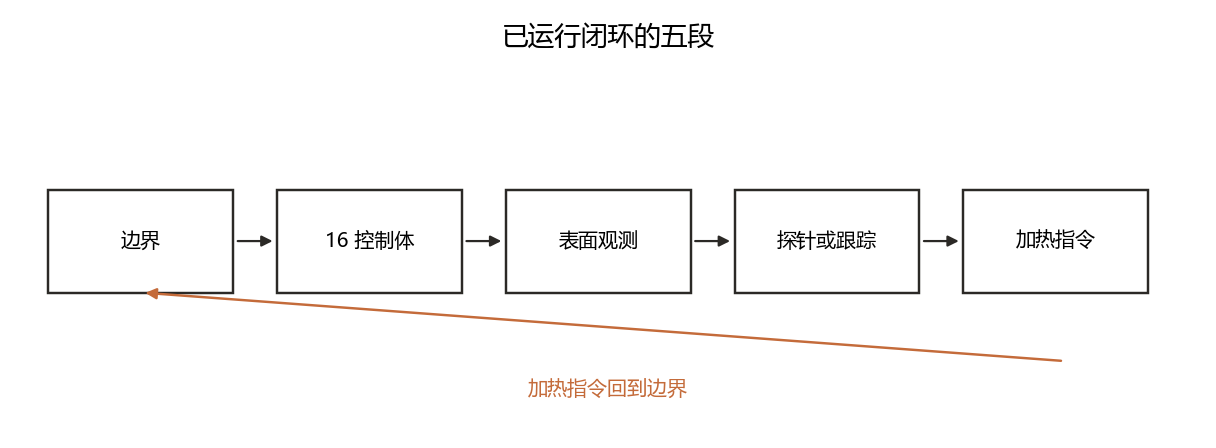
\includegraphics[width=\textwidth]{paper/M_loop.png}
\caption{评分核里实际走通的五段。加热指令回到边界。结构方程、集合滤波和预测控制求解器不在这五段里。}
\end{figure}

\begin{figure}[ht]
\centering
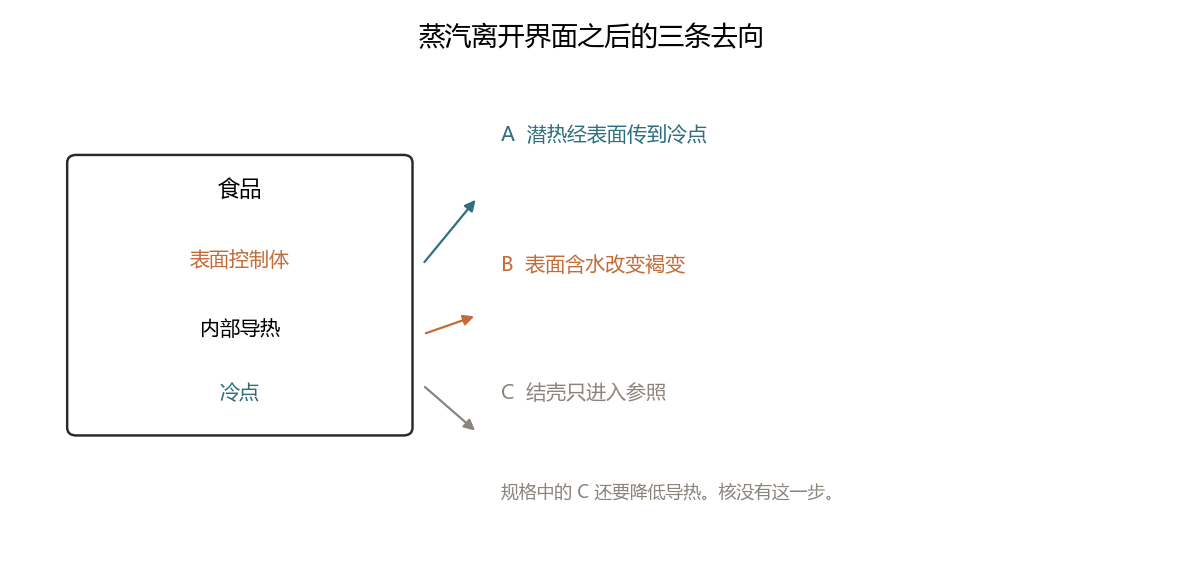
\includegraphics[width=0.92\textwidth]{paper/M_paths.png}
\caption{蒸汽离开表面之后，规格里有三条去向。核里路径 C 只进入热阻参照，不改变控制体导热。}
\end{figure}

\paragraph{本节不能推出的结论}
画出闭环不能推出每一步都有独立进程。合同约束的是数据依赖，不是部署拓扑。

\section{五层}

\paragraph{要判定的量}
每一层的输入里是否含有它不该读的对象。含有则该层的输出不能进入下一层。

\begin{description}
\item[L1 过程] 腔体几何、加热、蒸汽、风机、食品几何与初始场。仿真中由积分器充当。该层不含估计。本次积分器没有单独的腔体流动场。
\item[L2 多尺度模型] 把过程压缩为决策状态的演化。压缩必须保留冷点、表面干耗和局部过热。十六条控制体保留了冷点（最低温度）和表面温度，没有保留温度标准差的决策项。
\item[L3 结构孪生] 保存父节点固定的结构方程和参数后验。本次核没有这一层的积分。
\item[L4 对偶决策] 计算信息价值、品质价值，并选择动作。学习模块只允许在这一层。本次对偶策略是固定时间窗加饱和线性请求，不是信息增益的最大化。
\item[L5 安全执行] 电气、热、腔压、门封，以及只依赖这些测量的投影。这一层不调用网络。本次只有加热器温度进入削减。
\end{description}

执行器接口只有一个。动作进入接口之前带有标记：信息、品质或降级保温。标记决定它来自哪一个目标函数，不决定它能否绕过投影。核里的模式整数 \(0,1,2\) 就是这个标记的退化形式：品质、探针、保持。保持时请求降到 \(0.15\)，仍然经过同一条加热器更新。

\paragraph{本节不能推出的结论}
五层划分不能推出 L4 的网络已经训练。学习模块缺席时，L4 必须退回声明过的物理降阶，而不是保留上一次网络输出。

\section{四个时间尺度}

\paragraph{要判定的量}
慢计算是否能够关闭快保护。若能，架构不成立。

\begin{table}[ht]
\centering
\caption{尺度及允许的计算}
\begin{tabularx}{\textwidth}{llX}
\toprule
尺度 & 量级 & 允许的计算 \\
\midrule
电气切断 & 毫秒至 10 ms & 漏电、过流，无处理器 \\
热安全 & 0.1--1 s & 超温、干烧、腔压 \\
估计与动作 & 1--5 s & 滤波、信息价值、一次动作 \\
品质演化 & 10 s 至数十分钟 & 反应进度与预测时域 \\
跨次更新 & 一次过程结束 & 精度提高才写回类别先验 \\
\bottomrule
\end{tabularx}
\end{table}

快环可以中断慢环。慢环不能关闭快环。学习模块超时，则保持上一次已经投影的执行量，不保持网络的最后一次原始输出。

界面冷凝、蒸发的时间尺度是秒，冷点导热的时间尺度是分钟。动作设计利用这个分离：短脉冲改变表面节点，几乎不推动冷点进度。附录 \ref{app:scales} 用 \(\alpha=2.0\times 10^{-7}\,\mathrm{m}^2/\mathrm{s}\) 和 40 s 窗口算出 30 mm 的 Fourier 数为 \(8.9\times 10^{-3}\)。种子 7 的冷点在这 40 s 内从 \(8.01^\circ\mathrm{C}\) 到 \(8.05^\circ\mathrm{C}\)，与这个分离同方向。同方向不是对真实食品扩散率的测定。

本次时间步是 2 s，落在“估计与动作”的量级里，没有毫秒级的漏电回路。因此电气切断是规格，不是这次步进已经包含的动力学。

\begin{figure}[ht]
\centering
\begin{tikzpicture}[
  box/.style={draw, rounded corners, align=center, font=\small, inner sep=3pt, minimum width=32mm},
  arr/.style={-{Stealth}}
]
\node[box] (e) {电气切断};
\node[box, right=8mm of e] (h) {热安全};
\node[box, right=8mm of h] (a) {估计与动作};
\node[box, right=8mm of a] (q) {品质演化};
\draw[arr] (e)--(h);
\draw[arr] (h)--(a);
\draw[arr] (a)--(q);
\draw[arr, dashed] (h.south) -- ++(0,-0.6) -| (e.south);
\end{tikzpicture}
\caption{时间尺度的依存关系图，不是测量。实线是允许的调用方向。虚线表示快环可以中断慢环；慢环没有指向快环的关闭边。}
\end{figure}

\paragraph{本节不能推出的结论}
尺度分离不能推出任意短的蒸汽都无害。表面褐变和表面浸湿仍要进损伤预算。预算约束的是 \(\alpha_b\) 和 \(\varepsilon_{l,s}\)，不是冷点温度是否“看起来没变”。

\section{模块合同}

\paragraph{要判定的量}
模块之间传递的是分布还是一个点。把均值当成确定值，合同视为被破坏。

\begin{center}
\begin{tabularx}{\textwidth}{llX}
\toprule
模块 & 读入 & 写出 \\
\midrule
\texttt{sensor\_bus} & 物理量时序 & 带时间戳和不确定度的观测 \\
\texttt{manifold} & 观测、类别先验 & 集合或混合后验 \\
\texttt{dual\_policy} & 后验、执行器约束 & 标记过的动作 \\
\texttt{causal\_twin} & 后验、候选干预 & 轨迹与路径差 \\
\texttt{shield} & 候选动作、安全测量 & 投影后的执行量 \\
\texttt{knowledge} & 充分统计量 & 仅当精度提高时的新先验 \\
\bottomrule
\end{tabularx}
\end{center}

本次核没有这些模块名。对应关系是：观测在时间步内现场生成；后验退化成一个 \(\hat r\)、一个方差和一个 \(\hat T_c\)；策略直接写请求；没有因果模块；加热器削减代替投影；没有跨次写回。退化之后，下游仍然不应该把 \(\hat T_c\) 当成真值冷点。种子 7 在 1200 s 时估计 \(63.8^\circ\mathrm{C}\)、冷点 \(46.7^\circ\mathrm{C}\)，估计高于冷点。停机判据若把估计当成真值，就会在进度未到设计线时转入保持。该轨迹在 1680 s 正是这样：估计 \(85.85^\circ\mathrm{C}\)，冷点 \(73.0^\circ\mathrm{C}\)，\(\alpha_m=0.755\)。

\paragraph{本节不能推出的结论}
合同表不是软件目录已经实现的证明。缺模块时，正文只能写规格和退化路径，不能写该模块的误差指标。

\section{腔体上的最小执行与观测}

\paragraph{要判定的量}
信息动作是否需要额外机械机构。若不需要，探针必须能由已有的加热、蒸汽、热风和排汽组成。

\paragraph{继承的文献层与不继承的层}
继承的是边界条件进入食品的方式：对流、辐射和相变潜热 \cite{datta2007}。不继承某一腔体的风道尺寸。不继承把穿刺探针列为系统可重构性的必要条件。

过程载体是同一腔体内可切换的背部或顶部加热、蒸汽入口、热风、排汽阀。被动观测为腔温、腔湿、排气温度、加热功率、蒸汽功率与水位、门状态、漏电、壳体温度。食品侧为底部质量、门侧热像或一维热电堆。穿刺温度只作为对照通道。

蒸与烤的执行器已经覆盖短时边界组合。P4 的两段——先冷凝方向、再排汽高风——不增加阀门，只改变已有阀门的目标函数和时序。湿度调节最小化湿度误差；信息动作最大化参数信息。日志要记录这一时刻哪一个函数产生了指令。

本次核的执行量是加热、蒸汽和风机三个数。排汽没有独立变量，它被吸收进“蒸汽关闭且风机升高”。水位、门、漏电、腔压没有状态。因此“最小执行”在核里只覆盖加热与气流两路的一部分。

\paragraph{本节不能推出的结论}
执行器种类足够，不能推出探针库已经在线打分。固定时间窗是库的一个元素的时间表，不是 \(\argmax(G-\lambda C)\)。

\chapter{多尺度食品热状态：从多孔介质到决策流形}
\label{ch:physics}

本章要判定的量是：停机、探针和解释至少要看见哪几个场，以及哪一组泛函足够支撑这些决定。判定失败的表现是把“中心温度到了”写成品质，或把十六条控制体的工程通量写成多孔介质方程的解。

\section{计算域与状态}

\paragraph{要判定的量}
食品区域与腔体区域的边界上，哪些量属于食品状态，哪些量只作为边界输入。

\paragraph{继承的文献层与不继承的层}
体积分数的三相分解继承多孔介质平均 \cite{whitaker1977}。食品加工中的用法继承 \cite{datta2007}。不继承在孔隙尺度上跟踪每一个弯月面。不继承把腔体气体的速度场并进食品未知量。

食品区域 \(\Omega_f\subset\R^3\)，腔体气体区域 \(\Omega_c\)，交界面 \(\Gamma=\partial\Omega_f\)。时间 \(t\in[0,t_f]\)。体积分数满足
\begin{equation}
\varepsilon_s+\varepsilon_l+\varepsilon_g=1,\qquad \varepsilon_s=\varepsilon_s(S)>0.
\end{equation}
\(S(\vect{r},t)\) 综合收缩、孔隙闭合与表面结壳。它不是某一个分子机理的别名。

\begin{definition}[全场状态]
\label{def:fullstate}
\begin{equation}
\label{eq:state}
\vect{X}(\vect{r},t)=\big(T,\,p_g,\,\varepsilon_l,\,\omega_v,\,\vect{\alpha},\,S\big).
\end{equation}
\(T\) 为温度，\(p_g\) 为气相压力，\(\varepsilon_l\) 为液态水体积分数，\(\omega_v\) 为气相中水蒸气质量分数。反应进度
\begin{equation}
\vect{\alpha}=(\alpha_p,\alpha_g,\alpha_b,\alpha_m)\in[0,1]^4
\end{equation}
依次是蛋白质变性、淀粉糊化、美拉德褐变与微生物致死当量的归一化进度。
\end{definition}

腔体状态不进入食品场，而作为边界输入 \((T_\infty,Y_\infty,\vect{v}_\infty,\dot m_{\mathrm{st}},P_{\mathrm{heat}})\)。这个划分决定了在线模块可以读取的量：边界输入是执行器，不是食品的隐藏状态。

\paragraph{本节不能推出的结论}
写出全场，不能推出本次积分器推进了 \(p_g\) 和 \(\omega_v\)。那两个分量在十六条控制体里没有独立未知量。

\subsection{从代表体元到决策量}

代表体元上的平均把孔隙里的弯月面收成体积分数。决策不读取这个平均场的每一点，只读取九个泛函：冷点温度、表面平均温度、温度标准差、平均液相、表面液相、致死当量、表面褐变、结壳和失重。记这个向量为 \(\vect{z}\)。停机看的是 \(\vect{z}\) 里的冷点和致死当量，不看全场的 \(L^2\) 范数。

这条收缩有一个不能省略的条件：冷点的位置如果随脂肪夹层移动，取几何中心的温度就不是冷点。一维核把冷点定义成十六个控制体的最低温度，所以夹层可以把最低温度从对称面挪开。二维脂肪几何没有运行，不能把这个定义写成已经覆盖烤箱里的冷点云。

\section{宏观：热与三相质量}

\paragraph{要判定的量}
能量方程里必须保留的项，以及相变能不能写成无限快的代数约束。

\paragraph{继承的文献层与不继承的层}
继承体积平均后的能量、液相和蒸汽方程的结构 \cite{whitaker1977,datta2007}。不继承局部热非平衡：固、液、气在一个代表体元内用同一个 \(T\)。这个简化在蒸烤的分钟尺度上可接受，在秒级冷凝膜上只是近似。不继承某一干燥器的对流通量闭合。

忽略热局部非平衡时，
\begin{equation}
\label{eq:energy}
(\rho c)_{\mathrm{eff}}\frac{\partial T}{\partial t}
=\nabla\!\cdot\!\big(k_{\mathrm{eff}}\nabla T\big)
-\sum_{i\in\{l,v,a\}}\nabla\!\cdot\!(h_i\vect{n}_i)
-\dot m_{\mathrm{phase}}\,\Delta h_{\mathrm{vap}}
+q_{\mathrm{reac}}.
\end{equation}
右端四项依次是导热、流体携带的显热、相变潜热和反应热。有效容积热容与导热随 \(\varepsilon_l\) 和 \(S\) 变化，因此同一块食品在表面变干后导热下降。这是外干内生的机制，不是边界条件的附加说明。

液相与蒸汽：
\begin{align}
\label{eq:liquid}
\frac{\partial(\varepsilon_l\rho_l)}{\partial t}
&=-\nabla\!\cdot\!\vect{n}_l-\dot m_{\mathrm{phase}},\\
\label{eq:vapor}
\frac{\partial(\varepsilon_g\rho_g\omega_v)}{\partial t}
&=-\nabla\!\cdot\!\vect{n}_v+\dot m_{\mathrm{phase}}.
\end{align}
通量由 Darcy 渗流与 Fick 扩散合成：
\begin{align}
\vect{n}_l&=-\rho_l\frac{k_{rl}K}{\mu_l}\nabla p_l,\\
\vect{n}_v&=-\rho_g\omega_v\frac{k_{rg}K}{\mu_g}\nabla p_g
-\rho_g D_{\mathrm{eff}}\nabla\omega_v.
\end{align}
相变保持有限速率。无限快约束会把任何温度残差直接折成水分残差，使探针无法分开热阻和含水。
\begin{equation}
\label{eq:phase}
\dot m_{\mathrm{phase}}
=K_{\mathrm{ev}}\,a_w(\varepsilon_l,T)\,
\big(p_{\mathrm{sat}}(T)-p_v\big)_+
-K_{\mathrm{cd}}\,(p_v-p_{\mathrm{sat}}(T))_+.
\end{equation}
蒸制时腔体蒸汽压高，冷凝项在表面释放潜热。烤制时蒸汽压低，蒸发项吸热并留下干壳。符号由 \(p_v-p_{\mathrm{sat}}\) 决定，不由“当前模式叫做蒸还是烤”决定。

干空气通量与 \eqref{eq:vapor} 对称，相变源项改号。气相总压由状态方程闭合。这些闭合留在规格里。本次核没有压力未知量，界面潜热被收成
\begin{equation}
q_{\mathrm{lat}}=18000\,u_{\mathrm{st}}(1-a_w)-9000\,(1-u_{\mathrm{st}})\max(a_w-0.35,0)\,u_{\mathrm{fan}}.
\end{equation}
蒸汽指令直接决定符号，活度只调制幅度。这保留了“冷凝放热、蒸发吸热”的方向，没有保留 \eqref{eq:phase} 对局部蒸汽压的依赖。

\subsection{第一步表面温升}

种子 7 在 \(t=0\) 的表面温度是 \(11.361^\circ\mathrm{C}\)，冷点仍是 \(8^\circ\mathrm{C}\)。这个数可以由第一步的通量算出来，不必另找机制。

对偶策略在探针之前，风机是 \(0.4\)，蒸汽是 \(0\)，加热请求是 \(1\)。换热系数 \(h=12+55\times 0.4=34\)。环境温度 \(T_\infty=90+95\times 1=185^\circ\mathrm{C}\)。初含水 \(0.72\) 时肉糜活度被夹到 \(0.99\)，潜热通量
\[
q_{\mathrm{lat}}=-9000\times(0.99-0.35)\times 0.4=-2304\ \mathrm{W}/\mathrm{m}^2.
\]
进入表面的总通量
\[
q=h(T_\infty-8)+q_{\mathrm{lat}}+7000=34\times 177-2304+7000=10714\ \mathrm{W}/\mathrm{m}^2.
\]
表面控制体的厚度 \(\Delta x=0.030/16\)。一步 \(\Delta t=2\,\mathrm{s}\) 的温升
\[
\Delta T=\frac{q\,\Delta t}{(\rho c)\,\Delta x}=\frac{10714\times 2}{3.4\times 10^{6}\times 0.001875}=3.361\ \mathrm{K}.
\]
\(8+3.361=11.361\)。与 CSV 第一行的表面温度一致。内部节点在这一步还没有收到扩散，冷点保持 \(8^\circ\mathrm{C}\)。

估计冷点不使用这个更新后的表面。观测器先读到带 \(0.4\,\mathrm{K}\) 噪声的初始表面，再被上限剪到表面之下 \(16\,\mathrm{K}\)，所以第一行的估计是 \(-7.92^\circ\mathrm{C}\)。负值是这条上限，不是零下的传感器。

\subsection{十六条控制体上实际推进的格式}

规格保留气相压力和蒸汽质量分数。评分核只推进温度和含水。厚度 \(L\) 分成 \(n=16\) 段，\(\Delta x=L/16\)。内部节点的显式步是
\begin{equation}
\label{eq:fv-interior}
T_i^{k+1}=T_i^k+\alpha_i\Delta t\,\frac{T_{i+1}^k-2T_i^k+T_{i-1}^k}{(\Delta x)^2}.
\end{equation}
基准 \(\alpha=2.0\times 10^{-7}\,\mathrm{m}^2/\mathrm{s}\)。非均质档 2 只把下标 5 的导热改为 \(0.45k\)，所以该控制体的 \(\alpha\) 也是 \(0.45\) 倍。显式格式要求内部 Fourier 数小于二分之一：
\begin{equation}
\label{eq:fv-fo}
\frac{\alpha\Delta t}{(\Delta x)^2}<\frac12
\quad\Rightarrow\quad
\Delta t<\frac{(\Delta x)^2}{2\alpha}.
\end{equation}
代入三档厚度，上界分别是 2.20 s、8.79 s、24.41 s。战役步长是 2 s。15 mm 用到上界的大约 0.91。这个上界来自内部三点模板：自系数是 \(-2\alpha/(\Delta x)^2\)。表面上的模板少一个邻居，自系数是 \(-\alpha/(\Delta x)^2-h/((\rho c)\Delta x)\)。风机 0.4、\(h=34\) 时，15 mm 边界允许的步长约 8.4 s，30 mm 约 32 s，50 mm 约 84 s，都松于内部上界。把这一步写成矩阵，15 mm、\(h=34\)、\(\Delta t=2\,\mathrm{s}\) 的谱半径是 0.9989，最负实部是 \(-0.803\)；风机升到 1.3 时最负实部仍是 \(-0.803\)，前四位小数不变。最负的那个模态来自内部差分，边界对流没有把它推出单位圆。30 mm 和 50 mm 的谱半径分别是 0.9996 和 0.9998，最负实部已经是正的。网格减半的比较没有运行，所以这里不声明截断误差已经低于某一阈值。

串联热阻可以核对夹层的量级。均匀时十六段各为 \(\Delta x/k\)。把一段改为 \(\Delta x/(0.45k)\)，多出来的部分是
\begin{equation}
\label{eq:fv-fat}
\frac{\Delta R}{R}=\frac{1/0.45-1}{16}=0.076.
\end{equation}
夹层使总导热热阻增加约 7.6\%。这是一维串联的算术，不是一块脂肪几何的有效导热率。

\subsection{表面失水到不了褐变门限}

褐变增量和结壳增量都写成表面含水的门限。褐变要求 \(m_0<0.55\) 且 \(T_0>110^\circ\mathrm{C}\)。结壳要求 \(m_0<0.45\)。S1 的初始含水不低于 0.64。要看的是这一步能不能把表面含水降过这两条线。

含水的内部扩散系数是 \(D=2\times 10^{-9}(1+3m)\,\mathrm{m}^2/\mathrm{s}\)。表面控制体上的失水先写成一个无量纲强度
\begin{equation}
\label{eq:mloss}
\ell=1.6\times 10^{-4}\max(a_w-0.4,0)\,(0.3+u_v)\,(1-u_{\mathrm{st}}),
\end{equation}
再除以 \(\Delta x/L=1/16\)，最后乘 \(D\)。场还均匀时，相邻控制体的差分为零，表面含水的变化率只剩
\[
\dot m_0=-16\,D\,\ell.
\]
种子 7 的第一步，\(m=0.72\)，肉糜活度被裁到 0.99，风机 0.4，蒸汽为 0：\(\ell=6.61\times 10^{-5}\)，\(D=6.32\times 10^{-9}\)，\(\dot m_0=-6.7\times 10^{-12}\,\mathrm{s}^{-1}\)。乘上 3300 s，下降约 \(2\times 10^{-8}\)。S1 上更干、风更大的一格（含水 0.64、风机 1.3、无蒸汽）也只有 \(1.4\times 10^{-11}\,\mathrm{s}^{-1}\)。内部扩散只在控制体之间搬运水，不增加离开表面的净损失。因此 19440 行的终点 \(\alpha_b\) 都是精确的 0，结壳变量也停在 0。路径 C 里“结壳改变导热”的那一支没有进入这次积分；\(r_{\mathrm{proxy}}\) 里的 \(2.5S\) 同样是 0。

种子 7 的平均含水从第一行到最后一行都打印成 0.72，与这个量级一致。活度在三档战役含水上已经饱和，食材之间的差别还要再小一层：含水根本没有移动，活度曲线的形状没有机会被积分读到。

\paragraph{本节不能推出的结论}
\eqref{eq:energy} 不能用本次核的温度曲线来核对，因为核没有单独的 \(\dot m_{\mathrm{phase}}\) 场。核对 \eqref{eq:energy} 需要带压力和蒸汽分数的真值积分，本次没有运行。\eqref{eq:fv-fo} 只约束这一次选用的步长，不证明 15 mm 的结果对网格无关。失水率的量级也不能推出真实肌肉在 55 min 内不干燥：\(1.6\times 10^{-4}\) 是这条格式的系数，不是测量到的传质系数。

\section{界面：腔体如何进入食品}

\paragraph{要判定的量}
一次边界动作改变的是 \(T_\infty\) 一个数，还是能量边界的主项。

\paragraph{继承的文献层与不继承的层}
继承对流、辐射与潜热并列的界面能量平衡 \cite{datta2007,feyissa2013}。不继承把辐射收成一个等效环境温度而不记录角系数。

\begin{equation}
\label{eq:bc}
-k_{\mathrm{eff}}\nabla T\!\cdot\!\vect{n}
=h\big(|\vect{v}_\infty|\big)\,(T-T_\infty)
+\epsilon\sigma(T^4-T_w^4)
+\dot m_{\Gamma}\Delta h_{\mathrm{vap}}.
\end{equation}
\(h\) 随风速切换。表面冷凝时，潜热项的符号与干对流相反。蒸汽探针携带信息，是因为它改变 \eqref{eq:bc} 的主项，而不只是把 \(T_\infty\) 提高几度。

质量边界：液态水不穿过 \(\Gamma\)；蒸汽通量与腔体湿度差成正比；冷凝液作为表面 \(\varepsilon_l\) 的源。排汽阀打开时腔体湿度下降，蒸发恢复。漏汽在模型里是湿度偏差和门封热流，不单列成故障文案。

本次核的第一控制体通量为
\begin{equation}
q=h(T_\infty-T_0)+q_{\mathrm{lat}}+7000\,u,\qquad h=12+55\,u_{\mathrm{fan}},\qquad T_\infty=90+95\,u.
\end{equation}
辐射没有 \(T^4\) 项，被吸收进 \(7000\,u\) 和 \(T_\infty\) 对加热指令的线性关系。因此核可以比较“蒸汽开”和“蒸汽关”的方向，不能比较角系数或发射率。

\paragraph{本节不能推出的结论}
界面公式不给出腔体流场。\(h(|v|)\) 的查表属于尚未运行的边界库。

\section{介观与微观：反应进度不是温度的别名}

\paragraph{要判定的量}
同一条中心温度曲线能否对应不同的表面褐变和不同的热力进度。若能，停机不能定义成 \(T>T^\star\)。

\paragraph{继承的文献层与不继承的层}
速率形式继承 \cite{vanboekel2008}。等效时间继承 \cite{holdsworth1997}。不继承某一微生物的 \(D\) 值作为本文的认证限。活化能的数量级可以扫描，本次没有做这个扫描。

\begin{equation}
\label{eq:kinetics}
\frac{\partial\alpha_i}{\partial t}
=A_i\exp\!\Big(-\frac{E_{a,i}}{RT}\Big)
(1-\alpha_i)^{n_i}\,g_i(\varepsilon_l,S).
\end{equation}
\(g_p\) 在自由水不足时下降，\(g_g\) 只在淀粉与自由水同时存在时非零，\(g_b\) 在低水分、高温时上升。三个开关使表面褐变和内部变性可以分离。

热力进度不另造机理：
\begin{equation}
\label{eq:F}
\frac{\mathrm{d}F}{\mathrm{d}t}=10^{(T_{\mathrm{cold}}-T_{\mathrm{ref}})/z},\qquad
\alpha_m=1-\exp(-F/F_{\mathrm{req}}).
\end{equation}
\(T_{\mathrm{cold}}(t)=\operatorname{ess\,inf}_{\vect{r}\in\Omega_f}T(\vect{r},t)\)。冷点允许随边界移动。本次核取十六条控制体的最低温度，参考温度 \(70^\circ\mathrm{C}\)，\(z=10\,\mathrm{K}\)，\(F_{\mathrm{req}}=2\,\mathrm{min}\)。设计线 \(\alpha_m=0.85\) 对应 \(F=3.794\,\mathrm{min}\)，见附录 \ref{app:scales}。这条线是比较策略用的零点，不是认证阈值。

结构演化：
\begin{equation}
\label{eq:structure}
\frac{\partial S}{\partial t}
=\kappa_s(1-S)\,\langle\alpha_p-\alpha_s^\star\rangle_+
+\kappa_c\,\langle M_{c}- \varepsilon_l\rangle_+.
\end{equation}
第一项是蛋白收缩，第二项是干燥结壳。\(S\) 回调导热、渗透率和界面换热。耦合是闭环的：干壳降低内部升温速度，使 \(\alpha_m\) 落后于表面 \(\alpha_b\)。核里的结壳只在表面含水低于 \(0.45\) 时以 \(1.5\times 10^{-4}\,\mathrm{s}^{-1}\) 增长，并且只进入热阻参照，不改导热场。规格中的路径 C 因此没有在核里闭合。

\paragraph{本节不能推出的结论}
\(\alpha_m\) 的定义不包含微生物的初始数量。初始数量不进入状态。表面褐变公式里的 \(2\times 10^{-4}\) 是工程系数，不是 \eqref{eq:kinetics} 的 \(A_i\) 与 \(E_{a,i}\)。

\section{决策流形：估计什么，不估计什么}

\paragraph{要判定的量}
全场的哪些泛函进入控制器。进一步细化网格若不能改变已投影的安全动作，就不必实时重构到网格精度。

\paragraph{继承的文献层与不继承的层}
继承“控制器只依赖 Lipschitz 代价”这一优化事实 \cite{rawlings2017}。不继承把降阶误差设成零。

\begin{definition}[决策状态]
\label{def:decision}
\begin{equation}
\label{eq:z}
\vect{z}(t)=\big(
T_{\mathrm{cold}},\,
\bar T_s,\,
\sigma_T,\,
\bar\varepsilon_l,\,
\varepsilon_{l,s},\,
\alpha_m,\,
\alpha_{b,s},\,
S_s,\,
m_{\mathrm{loss}}
\big).
\end{equation}
依次为冷点温度、表面均温、温度场标准差、平均液相分数、表面液相分数、致死进度、表面褐变、表面结壳与累计质量损失。
\end{definition}

\begin{proposition}[决策充分性]
若阶段代价与约束都是 \(\vect{z}\) 的 Lipschitz 函数，并且 \(\vect{z}\) 的后验不确定度低于该 Lipschitz 常数所对应的阈值，则进一步细化网格场不会改变已投影的安全动作。
\end{proposition}

论证分三步。第一，动作是代价的 \(\epsilon\)-最优解。第二，代价对 \(\vect{z}\) 的变化由 Lipschitz 常数控制，后验期望之差不超过该常数乘不确定度。第三，期望之差小于动作切换的滞回带时，投影后的执行量不变。滞回带属于决策层，安全不等式属于执行层，二者不共用阈值。因此增加红外像素而 \(\vect{z}\) 的分位区间不变时，执行量保持不变。

全场到 \(\vect{z}\) 的映射记为 \(\Phi\)。在线模型可以是一维径向多孔介质、两节点热容网络，或预计算的神经算子。三者必须在 \(\vect{z}\) 上可比。不允许只在腔温上对齐。神经算子本次没有训练。两节点只用于可辨识性。主日志来自一维十六条控制体，它给出 \(T_{\mathrm{cold}}\)、表面温度、平均含水和 \(\alpha_m\)，没有给出 \(\sigma_T\) 的决策项。

\paragraph{本节不能推出的结论}
命题不说明 Lipschitz 常数已经标定。未标定之前，不能用它裁剪传感器。

\section{两节点模型：后续辨识的工作方程}

\paragraph{要判定的量}
内部热阻能否在短时激励下与外部热阻分开。工作方程只保留这个判定所需的状态。

\paragraph{继承的文献层与不继承的层}
两节点是集总热容，不继承多孔介质的空间分辨率。它只作为探针分析的局部载体。全场方程负责尚未运行的离线真值。

表面节点 \(1\)、内部节点 \(2\)：
\begin{align}
\label{eq:twonode}
C_1\dot T_1
&=\frac{T_\infty-T_1}{R_{\mathrm{ext}}(v)}+\frac{T_2-T_1}{R_{\mathrm{int}}}
+q_{\mathrm{lat}}(\dot m_\Gamma),\\
C_2\dot T_2
&=\frac{T_1-T_2}{R_{\mathrm{int}}},\\
\dot m
&=-k_m\big(a_w(m)\,p_{\mathrm{sat}}(T_1)-p_\infty\big).
\end{align}
\(R_{\mathrm{ext}}\) 由风速与是否冷凝切换，\(R_{\mathrm{int}}\) 随结壳增大，\(C_1,C_2\) 随含水下降。\(q_{\mathrm{lat}}\) 在冷凝时为正、蒸发时为负。

无相变且 \(\dot m=0\) 时，平衡迫使 \(T_1=T_2=T_\infty\)，三个参数 \(R_{\mathrm{int}},C_1,C_2\) 从代数方程中消失。证明放在命题 \ref{prop:steady}。这里只记录使用方式：恒温段的腔温采样不更新内部热阻，信息动作必须离开平衡。

\subsection{状态可观测与参数不可辨识}

把含水冻结，相变通量为零，\eqref{eq:twonode} 对 \((T_1,T_2)\) 是线性的。记
\[
a=\frac{1}{C_1 R_{\mathrm{ext}}},\quad
b=\frac{1}{C_1 R_{\mathrm{int}}},\quad
c=\frac{1}{C_2 R_{\mathrm{int}}}.
\]
状态矩阵与观测矩阵为
\begin{equation}
\label{eq:fv-obsv}
\vect{A}=\begin{pmatrix}-a-b & b\\ c & -c\end{pmatrix},\qquad
\vect{C}=\begin{pmatrix}1 & 0\end{pmatrix}.
\end{equation}
可观测矩阵的两行是 \(\vect{C}\) 与 \(\vect{C}\vect{A}\)。第二行是 \((-a-b,\, b)\)。行列式等于 \(b\)。热容和内部热阻都取正时 \(b\neq 0\)，所以从表面温度看，两个温度状态是可观测的。

参数是另一件事。在平衡点 \(T_1=T_2=T_\infty\) 上，对 \(R_{\mathrm{int}}\) 的灵敏度满足齐次方程，初值为零，于是
\begin{equation}
\label{eq:fv-fisher0}
\frac{\partial T_1}{\partial R_{\mathrm{int}}}=\frac{\partial T_2}{\partial R_{\mathrm{int}}}=0.
\end{equation}
把这一列放进 \eqref{eq:fisher}，对应的信息是零。状态可观测，不推出内部热阻可辨识。辨识需要离开平衡的输入。这一段是线性化的代数，不是集合滤波器的运行记录。

\paragraph{本节不能推出的结论}
两节点上的秩条件通过，只说明判据方向。它不代替带 GAB、各向异性和脂肪层的真值。

\section{参数分层}

\paragraph{要判定的量}
哪些参数允许被一次烹饪改写。允许改写的范围决定了估计器的维数。

\begin{table}[ht]
\centering
\caption{参数：哪些锁死，哪些在线更新}
\begin{tabularx}{\textwidth}{lXll}
\toprule
符号 & 含义 & 来源 & 在线 \\
\midrule
\(p_{\mathrm{sat}}(T)\)、\(\Delta h_{\mathrm{vap}}\) & 水的物性 & 蒸汽表 & 否 \\
\(A_i,E_{a,i},n_i\) & 反应动力学 & 类别先验 & 弱更新 \\
\(k_{\mathrm{eff}},K,D_{\mathrm{eff}}\) & 有效传递 & 先验加本次 & 是 \\
\(R_{\mathrm{ext}},h(v)\) & 腔体边界 & 探针 & 是 \\
\(C_1,C_2,R_{\mathrm{int}}\) & 热容与内部热阻 & 探针 & 是 \\
\(K_{\mathrm{ev}},K_{\mathrm{cd}}\) & 相变弛豫 & 探针 & 是 \\
几何厚度 \(L\) & 冷点路径长度 & 视觉或给定 & 本次固定 \\
\bottomrule
\end{tabularx}
\end{table}

锁死蒸汽表，是为了不让残差网络用任意函数拟合潜热。本次核更窄：在线只更新一个无量纲热阻代理和它的方差。导热、潜热系数和反应除数都是常数。厚度由实验设计给定，不在线估计。

\paragraph{本节不能推出的结论}
“在线：是”表示规格允许更新，不表示本次日志里该参数有后验样本。

\section{非均质与界面的闭合关系}

\paragraph{要判定的量}
真值模型比两节点多出的闭合，哪些必须在在线参数之外单独写明，以免被吸收进一个等效热阻。

\paragraph{继承的文献层与不继承的层}
GAB 形式继承多层吸附的三参数结构 \cite{gab1980}。清洁拟合的数量级来自 \cite{sorption2026}，约束范围在第 \ref{ch:data} 章。组分加和的导热传统见 \cite{choi1986}，各向异性不在该加和之内。不继承把肉类活度写成这份等温线的测定。

水分活度
\begin{equation}
\label{eq:gab}
M=\frac{M_0\,C\,K\,a_w}{(1-K a_w)\,(1-K a_w+C K a_w)}.
\end{equation}
清洁子集上 \(X_m\) 的十分位、中位、九十分位约为 \(0.037\)、\(0.074\)、\(0.144\)，\(C\) 约为 \(4\)、\(11\)、\(45\)，\(K\) 约为 \(0.61\)、\(0.77\)、\(0.96\)。肉类条数为 0。土豆六条清洁曲线只到 \(60^\circ\mathrm{C}\)：吸附支的 \(X_m\) 从 \(30^\circ\mathrm{C}\) 的 \(0.057\) 降到 \(60^\circ\mathrm{C}\) 的 \(0.036\)，\(K\) 从 \(0.912\) 降到 \(0.762\)。方向与吸附热随温度下降一致，数值不能外推到烤制表面。

\begin{figure}[ht]
\centering
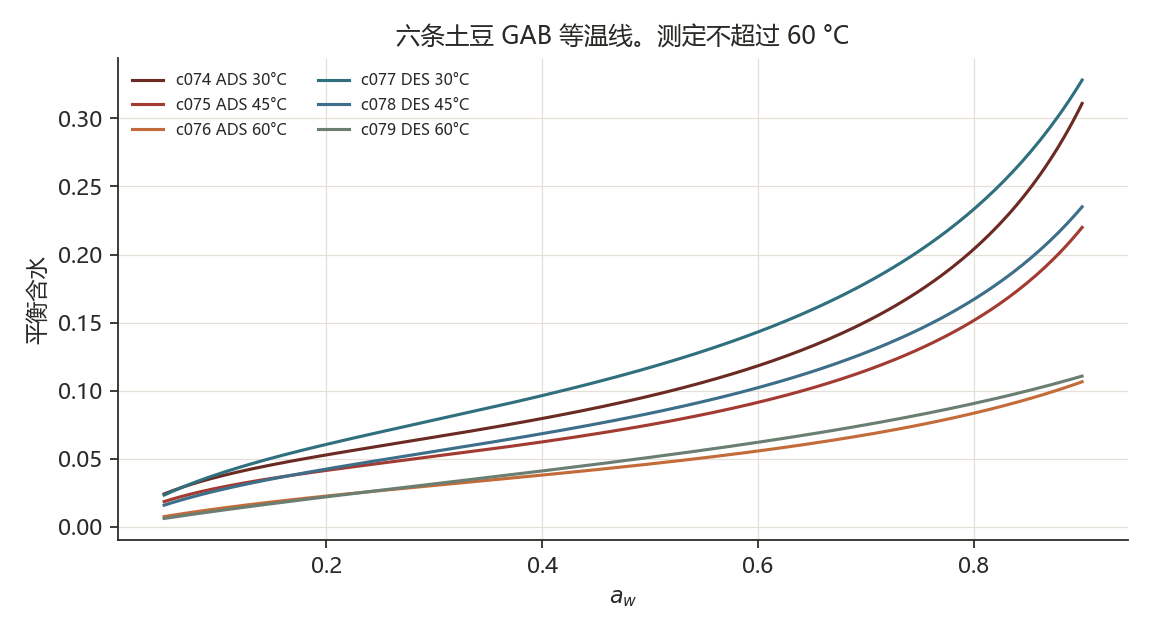
\includegraphics[width=0.9\textwidth]{paper/P_gab.png}
\caption{六条土豆清洁拟合在 \(a_w\in[0.05,0.90]\) 上的平衡含水。同一温度上脱附支高于吸附支。\(60^\circ\mathrm{C}\) 的两条曲线明显更低。测定温度不超过 \(60^\circ\mathrm{C}\)。}
\end{figure}

\begin{figure}[ht]
\centering
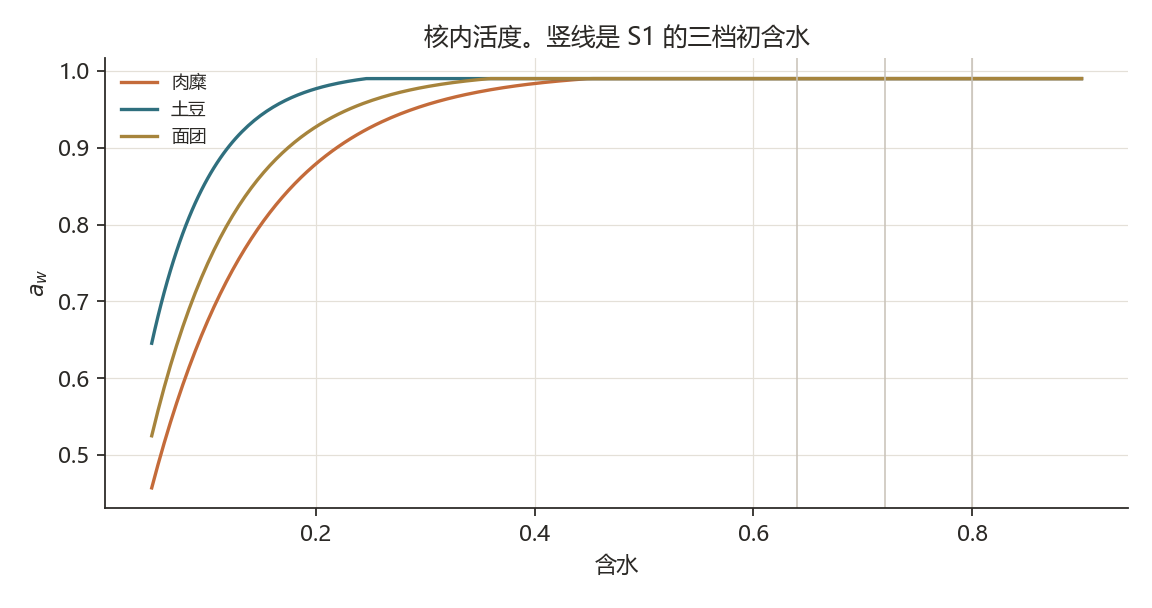
\includegraphics[width=0.88\textwidth]{paper/P_aw.png}
\caption{评分核的活度映射。竖线是 S1 的三档初含水。三条曲线在这三档上都贴近上界，所以食材因子在交叉表里几乎重合。}
\end{figure}

有效导热写成各向异性张量：
\begin{equation}
\label{eq:aniso}
\vect{k}_{\mathrm{eff}}=k_\perp(M,S)\,\vect{I}+(k_\parallel-k_\perp)\,\vect{e}\otimes\vect{e}.
\end{equation}
脂肪夹层作为并联热阻 \(R_{\mathrm{fat}}=L_{\mathrm{fat}}/(k_{\mathrm{fat}}A)\) 加到冷点路径上。冷点可以落在低导热层的背侧，而不必是几何中心。核里的非均质档 2 只把下标 5 的控制体导热乘 \(0.45\)，没有独立的脂肪几何，也没有纤维方向。

收缩：
\begin{equation}
\label{eq:shrink}
\dot L=-\beta_s L_0\,\dot\alpha_p,\qquad K=K_0\Big(\frac{L}{L_0}\Big)^{n_K}\varepsilon_g^{n_\varepsilon}.
\end{equation}
渗透率随孔隙与收缩一起变。核里的厚度在一条轨迹内是常数，收缩没有进入网格。

腔壁辐射用一个角系数：
\begin{equation}
q_{\mathrm{rad}}=F_{h,s}\epsilon_s\sigma(T_h^4-T_s^4)+F_{w,s}\epsilon_s\sigma(T_w^4-T_s^4).
\end{equation}
热像里的反射项与 \(F_{h,s}T_h^4\) 是同一几何量。核里没有这一项。

\paragraph{本节不能推出的结论}
闭合关系写在规格里，不能写成 S1 已经扫描了各向异性比或收缩指数。S1 的非均质只有两档：初始温度 \(\pm 4^\circ\mathrm{C}\)，以及一个控制体的导热系数。

\section{三个原型的方程差异}

\paragraph{要判定的量}
三个原型的差异来自哪一项开关，而不是来自三套互不相关的公式。

\begin{table}[ht]
\centering
\caption{原型开关}
\begin{tabularx}{\textwidth}{lXXX}
\toprule
项 & 肉糜 & 土豆 & 面团 \\
\midrule
主反应 & \(\alpha_p\) 与 \(\alpha_m\) & \(\alpha_g\)，需自由水 & \(\alpha_g\) 与后期 \(\alpha_b\) \\
等温线 & 开放区间，无公开肉类曲线 & 土豆清洁拟合，只到 \(60^\circ\mathrm{C}\) & 谷物清洁拟合的区间 \\
各向异性 & 文献区间，未在本次扫描 & 近似各向同性 & 气孔方向可有弱各向异性 \\
脂肪层 & 规格中可开启；本次只有一个低导热控制体 & 关闭 & 关闭 \\
收缩 & 规格开启；本次厚度固定 & 弱 & 体积变化作为已知几何，不反解 \\
\bottomrule
\end{tabularx}
\end{table}

核里三个原型共用同一套导热和进度公式。差别只在活度尺度：肉糜 \((0.10,0.70)\)，土豆 \((0.055,0.80)\)，面团 \((0.08,0.75)\)。交叉表里三个食材的中位误差几乎相同，与“原型只改了一个弱的活度尺度”一致。这不能用来声称蛋白与淀粉的反应差异已经被检验。

\paragraph{本节不能推出的结论}
面团膨胀不在状态里。把它反解进估计，会把发酵气体和热加工认知绑成一个问题。本次没有这样做，也不报告膨胀误差。

\section{无量纲结构与尺度分离}

\paragraph{要判定的量}
短探针的持续时间是否落在冷点 Fourier 数远小于 1 的窗口内。

取厚度 \(L\)、外部温差和初始液相分数。\(\mathrm{Fo}=\alpha t/L^2\) 衡量内部导热是否追上边界。\(\mathrm{Bi}=hL/k\) 衡量外部对流是否主导表面梯度。\(\mathrm{Ko}=\Delta h_{\mathrm{vap}}\varepsilon_{l0}\rho_l/((\rho c)_{\mathrm{eff}}\Delta T)\) 衡量潜热相对显热的大小。

用核的常数，40 s 窗口、30 mm 的 Fourier 数是 \(8.9\times 10^{-3}\)；风机 \(0.4\) 时 30 mm 的 Biot 数是 \(1.5\)。蒸制阶段界面冷凝使表面先跃迁，冷点仍由 Fourier 数控制。损伤预算因此主要写在表面褐变和表面含水上。厚度增大使内部时间常数增大，窗口更宽，但表面响应对内部热阻的灵敏度下降。信息增益存在上界；上界低于停机所需的熵减时，输出进度区间，不输出一个剩余时间点。本次没有计算这个上界的等高线。

\subsection{用已定常数算出的三张尺度图}

\begin{figure}[ht]
\centering
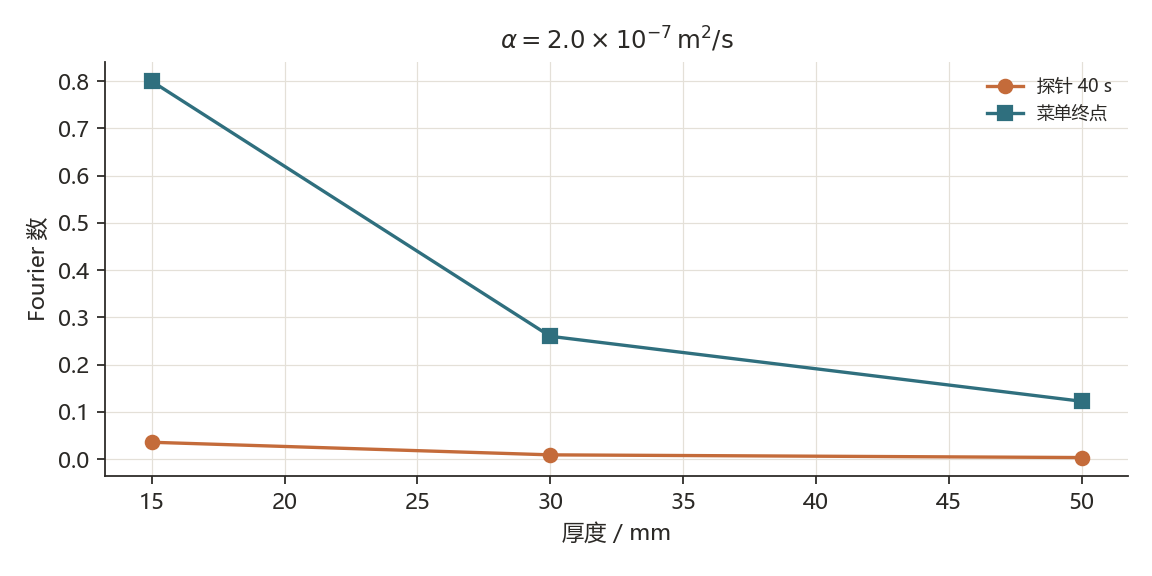
\includegraphics[width=0.88\textwidth]{paper/P_fo.png}
\caption{探针 40 s 与三档菜单终点的 Fourier 数。厚件在菜单终点仍远小于 1。\(\alpha\) 是核里的设定值。}
\end{figure}

\begin{figure}[ht]
\centering
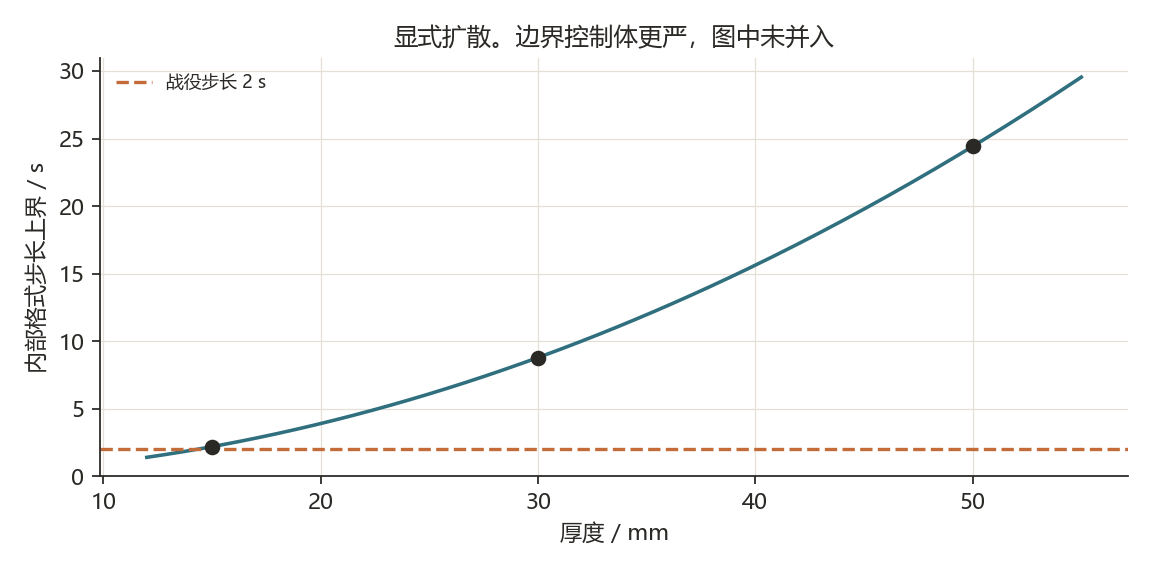
\includegraphics[width=0.88\textwidth]{paper/P_dt.png}
\caption{内部显式格式的步长上界。15 mm 处上界略高于战役使用的 2 s。边界对流项的上界更松，谱半径由内部差分决定。}
\end{figure}

\begin{figure}[ht]
\centering
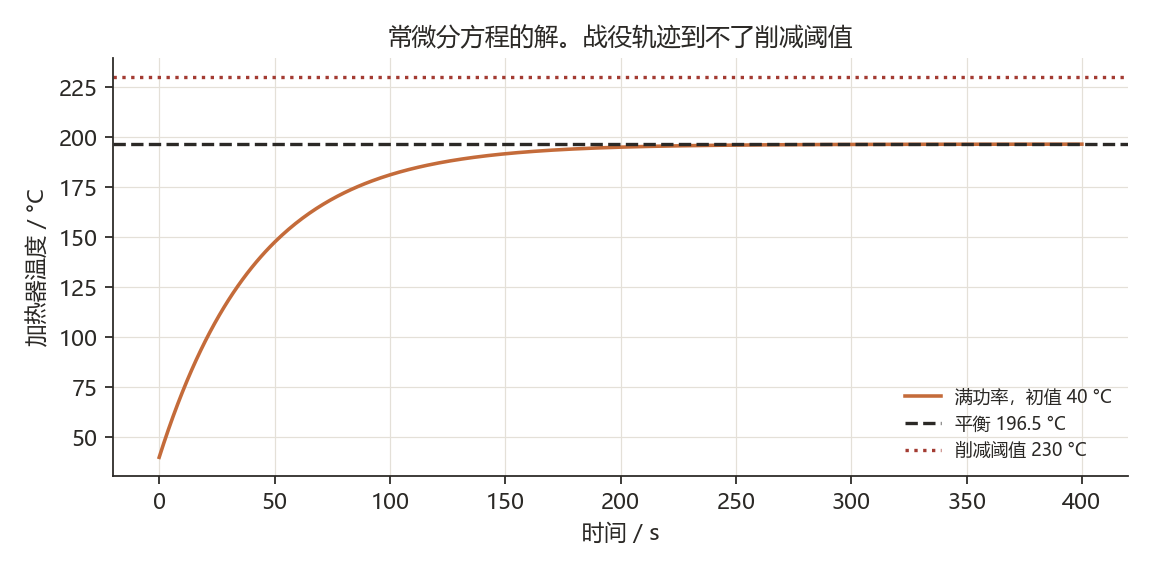
\includegraphics[width=0.88\textwidth]{paper/P_heater.png}
\caption{满功率加热器常微分方程从 \(40^\circ\mathrm{C}\) 出发，平衡在 \(196.5^\circ\mathrm{C}\)。削减阈值 \(230^\circ\mathrm{C}\) 在这条解上没有交点。}
\end{figure}

\subsection{常物性平板的本征根}

把核里的 \(\alpha\) 和 \(h\) 放进一块常物性、常换热、无潜热的平板，只为了给出线性对照。对照不是十六条格式的解。坐标从绝热面量到加热面，厚度仍是 \(L\)。无量纲温度 \(\theta\) 满足
\begin{equation}
\label{eq:slab}
\partial_{\mathrm{Fo}}\theta=\partial_{\xi\xi}\theta,
\qquad
\partial_\xi\theta\big|_{\xi=0}=0,
\qquad
\partial_\xi\theta\big|_{\xi=1}=-\mathrm{Bi}\,\theta(1).
\end{equation}
\(\xi=x/L\)，\(\mathrm{Fo}=\alpha t/L^2\)，\(\mathrm{Bi}=hL/k\)。分离变量 \(\theta=\cos(\zeta\xi)\,\mathrm{e}^{-\zeta^2\mathrm{Fo}}\) 放进加热面的边界条件，得到
\begin{equation}
\label{eq:slab-root}
\zeta\tan\zeta=\mathrm{Bi}.
\end{equation}
根落在 \((n\pi,\,n\pi+\pi/2)\)。均匀初温的系数由本征函数在 \([0,1]\) 上的权 \(\cos^2(\zeta\xi)\) 归一，第一项是
\begin{equation}
\label{eq:slab-A}
A_1=\frac{4\sin\zeta_1}{2\zeta_1+\sin 2\zeta_1}.
\end{equation}
第一项单独衰减的时间是 \(L^2/(\alpha\zeta_1^2)\)。下表的根用二分法求到 \(10^{-12}\) 量级，再四舍五入。

\begin{table}[ht]
\centering
\caption{常物性平板的前三个根。线性对照，不是核的轨迹。}
\begin{tabular}{lrrrr}
\toprule
条件 & \(\mathrm{Bi}\) & \(\zeta_1\) & \(\zeta_2\) & \(\zeta_3\) \\
\midrule
15 mm，风机 0.4 & 0.75 & 0.771 & 3.361 & 6.400 \\
30 mm，风机 0.4 & 1.50 & 0.988 & 3.542 & 6.510 \\
50 mm，风机 0.4 & 2.50 & 1.142 & 3.732 & 6.643 \\
30 mm，探针风机 1.3 & 3.68 & 1.245 & 3.899 & 6.781 \\
\bottomrule
\end{tabular}
\end{table}

对应的 \(A_1\) 是 1.097、1.154、1.197、1.224。第一项的时间：Bi \(=1.50\) 时，15 mm、30 mm、50 mm 分别是 1152 s、4608 s、12799 s。菜单终点的 Fourier 数是 0.80、0.26、0.12，都短于“第一项降到 \(1/\mathrm{e}\)”所需的 Fourier 数 1.02。六项截断下，中心剩余温差在探针窗口 \(\mathrm{Fo}=8.9\times 10^{-3}\)、Bi \(=1.50\) 时仍是 0.9997，表面剩余是 0.858。菜单终点上，15 mm（Bi \(=0.75\)，Fo \(=0.80\)）的中心剩余是 0.681，30 mm（Bi \(=1.50\)，Fo \(=0.26\)）是 0.887，50 mm（Bi \(=2.50\)，Fo \(=0.12\)）是 0.974。厚件在菜单时间上，常物性中心几乎还没动。这和交叉表里厚件开环停在进度下沿的方向相同。相同只说明尺度，因为核的腔温随加热指令从 \(90^\circ\mathrm{C}\) 变到 \(185^\circ\mathrm{C}\)，还有潜热项，初温也不必均匀。

\paragraph{本节不能推出的结论}
无量纲估计不能代替第 \ref{ch:sim} 章的策略比较。尺度使用的 \(\alpha\) 是设定值。更换 \(\alpha\) 之后的排序没有运行。本征根表不能读成种子 7 的剖面：那条轨迹的表面在 160 s 已经到 \(80^\circ\mathrm{C}\)，冷点仍在 \(8^\circ\mathrm{C}\)，驱动是随时间变化的通量，不是一次常 Bi 的阶跃。

\chapter{隐藏状态估计：观测算子、可辨识性与滤波}
\label{ch:est}

本章要判定的量是：被动观测对内部热阻的信息在什么条件下为零，以及在线估计器输出的是一个温度点还是决策状态的后验。规格中的估计器是分层的集合滤波。本次日志里的估计器是一个标量跟踪器。二者必须分开写。

\section{可安装观测}

\paragraph{要判定的量}
哪一些通道允许进入品质滤波，哪一些只进入安全约束。

\paragraph{继承的文献层与不继承的层}
观测算子的病态性继承 \cite{ozisik2000}。红外亮度里的发射与反射必须分开，否则加热管的辐射会被当成食品表面温度。不继承某一热像器件的样本噪声作为系统精度。

\begin{table}[ht]
\centering
\caption{进入品质估计器的观测}
\begin{tabularx}{\textwidth}{llX}
\toprule
通道 & 符号 & 与隐藏状态的关系 \\
\midrule
腔体空气温度 & \(y_T\) & 靠近 \(T_\infty\)，受加热器辐射污染 \\
腔体相对湿度 & \(y_\varphi\) & \(p_v/p_{\mathrm{sat}}(T_\infty)\)，饱和时丢失分辨率 \\
食品质量 & \(y_m\) & 累计蒸发的积分，不定位冷点 \\
表面热像 & \(\vect{y}_{\mathrm{IR}}\) & 发射率未知的辐射亮度 \\
电功率 & \(y_P\) & 已知输入，写入边界，不当作食品状态 \\
排气温度 & \(y_{T,e}\) & 冷凝与漏汽的积分证据 \\
\bottomrule
\end{tabularx}
\end{table}

\begin{definition}[观测方程]
\begin{equation}
\label{eq:obs}
\vect{y}_k=h\big(\Phi(\vect{X}(t_k)),\vect{\theta}\big)+\vect{v}_k.
\end{equation}
红外通道
\begin{equation}
\label{eq:ir}
L_j=\epsilon(\varepsilon_{l,s},S_s)\,\sigma T(\vect{r}_j)^4
+\big(1-\epsilon(\varepsilon_{l,s},S_s)\big)L_j^{\mathrm{refl}}.
\end{equation}
\end{definition}

发射率随表面变干下降。系统精度取发射率区间两端分别滤波后的分位包络，不取器件标称精度。本次核没有热像，也没有质量。进入跟踪器的是表面温度加 \(0.4^\circ\mathrm{C}\) 的确定性散列，以及平均含水加 \(0.004\) 的散列。噪声不是高斯抽样，重复运行得到同一轨迹。

\paragraph{本节不能推出的结论}
表中的通道是规格。没有采样的通道，不能在结果里出现“去掉该通道后误差上升”这一句。

\section{逆问题的病态结构}

\paragraph{要判定的量}
只加密表面像素，能否稳定恢复冷点。

\paragraph{继承的文献层与不继承的层}
线性化热方程在厚度方向上，对高频边界噪声的放大随 \(\mathrm{e}^{kL}\) 增长 \cite{ozisik2000}。不继承某一个正则化参数作为物理常数。

由此得到四条限制。只加密表面红外像素，不能稳定恢复冷点。必须有一个穿透时间尺度上的动态激励，或一个对内部热阻敏感的积分量。质量损失对累计蒸发敏感，对冷点位置不敏感。先验把解限制在决策流形附近，正则化来自物理，而不是一个随意的光滑惩罚。

\begin{proposition}[静态观测不足以分离内外热阻]
在 \eqref{eq:twonode} 中令三个导数为零且无相变。则 \(T_1=T_2=T_\infty\)，\(R_{\mathrm{int}}\)、\(C_1\)、\(C_2\) 全部从代数方程中消失。
\end{proposition}

完整证明在命题 \ref{prop:steady}。断言在 \(R\in\{1,3,6\}\)、\(T_\infty=100\) 上积分到平衡，温差极差为 0。这是“到时按菜单停机”失败的数学形式：菜单在稳态配方上标定，这一次的内部热阻从未被观察。

\subsection{可观测矩阵的行列式}

沿用 \eqref{eq:fv-obsv} 的两节点线性化。输出只取表面温度，
\[
\mathcal{O}=\begin{pmatrix}\vect{C}\\ \vect{C}\vect{A}\end{pmatrix}
=\begin{pmatrix}1&0\\ -a-b& b\end{pmatrix}.
\]
\[
\det\mathcal{O}=b=\frac{1}{C_1 R_{\mathrm{int}}}.
\]
\(C_1>0\) 且 \(R_{\mathrm{int}}\) 有限时，行列式不为零，两个温度状态可观测。\(R_{\mathrm{int}}\to\infty\) 时行列式趋于零，表面温度不再携带内部节点的信息。厚件在菜单终点的 Fourier 数远小于 1，对应的就是这个方向：不是秩突然消失，而是短时间内灵敏度很小。

平衡点上的参数灵敏度是另一件事。命题 \ref{prop:steady} 已经说明三个温度对 \(R_{\mathrm{int}}\) 的导数为零。把零列放进 \eqref{eq:fisher}，该项贡献是零。因此“状态可观测”不能写成“内部热阻已经可辨识”。探针的作用是离开平衡，让灵敏度列不再是零。

已实现的跟踪器没有组装 \(\mathcal{O}\)，也没有组装 Fisher 矩阵。它用一个标量时间常数跟随表面，再用 \(\hat r\) 把估计压低。方差只在 190 s 之后、而且新的 \(\hat r\) 更接近真值温差参照时，乘一次 0.35。这个参照用了表面与冷点的真值差，所以方差下降不是 \eqref{eq:fisher} 的特征值。

\paragraph{本节不能推出的结论}
病态性不意味着估计不可能。它意味着估计依赖激励和先验。没有激励时增加采样频率无效。

\section{动态可辨识性}

\paragraph{要判定的量}
相变项是否给输入矩阵增加一个与 \(T_\infty\) 线性无关的方向。对 \eqref{eq:twonode}，两列都只进入表面节点，方向共线；要分开的是 \(R_{\mathrm{ext}}\) 与 \(R_{\mathrm{int}}\) 的灵敏度列。

\paragraph{继承的文献层与不继承的层}
灵敏度方程和 Fisher 信息是局部可辨识性的标准构造。不继承本次已经算出了 Fisher 矩阵的特征值。该矩阵没有在日志里计算。

把 \eqref{eq:twonode} 在无相变工作点线性化，状态 \((\delta T_1,\delta T_2)\)，输入 \((\delta T_\infty,\delta v)\)。风速只进入 \(R_{\mathrm{ext}}\)。对输出 \(y=T_1\)，可观测矩阵的秩为 2，内部状态在结构上可观测，但 Gram 矩阵的条件数随 \(R_{\mathrm{int}}/R_{\mathrm{ext}}\) 增大而变坏。厚、干、结壳的食品，表面温度对冷点的响应又慢又弱。

相变项与腔温都写在表面节点的能量平衡上，输入列共线。短蒸汽脉冲仍然改变表面通量的大小，并且不经过 \(R_{\mathrm{ext}}\) 这个系数。参数灵敏度满足
\begin{equation}
\label{eq:sens}
\frac{\mathrm{d}}{\mathrm{d}t}\frac{\partial \vect{s}}{\partial\theta_i}
=\vect{A}(\vect{\theta})\frac{\partial \vect{s}}{\partial\theta_i}
+\frac{\partial \vect{A}}{\partial\theta_i}\vect{s}
+\frac{\partial \vect{B}}{\partial\theta_i}\vect{u},
\end{equation}
其中 \(\vect{s}=(T_1,T_2,m)\)。Fisher 信息
\begin{equation}
\label{eq:fisher}
\vect{\mathcal{I}}(\vect{\theta};\vect{u}_{0:K})
=\sum_{k=0}^{K}
\Big(\frac{\partial h}{\partial \vect{s}}\frac{\partial \vect{s}_k}{\partial\vect{\theta}}\Big)^{\!\top}
\vect{R}_k^{-1}
\Big(\frac{\partial h}{\partial \vect{s}}\frac{\partial \vect{s}_k}{\partial\vect{\theta}}\Big).
\end{equation}
探针设计在规格上最大化 \(\log\det\vect{\mathcal{I}}\) 的增量。断言没有组装这个矩阵。它只比较了两段脉冲与单独蒸汽的表面—内部滞后：\(40.846\) 与 \(38.912\)，判据是差值大于 1。差值大于 1 说明第二段改变了滞后，不说明 Fisher 矩阵的最小特征值已经上升。

\paragraph{本节不能推出的结论}
可观测秩为 2 是线性化结构的结论。它不给出厚件上的估计误差。厚件误差见交叉表，而且那个误差来自标量跟踪器，不是来自 \eqref{eq:fisher} 的实现。

\section{贝叶斯估计器}

\paragraph{要判定的量}
在线更新的是哪一层参数，控制器读的是均值还是分位数。

\paragraph{继承的文献层与不继承的层}
集合卡尔曼滤波的预测—分析结构继承 \cite{evensen2003}。不继承本次已经用 32 个成员跑完了主表。没有这次运行。

规格分三层。

\begin{enumerate}
\item 参数层。\(\vect{\theta}=(C_1,C_2,R_{\mathrm{int}},R_{\mathrm{ext}},k_m,K_{\mathrm{ev}})\)。先验按类别读取。过程噪声只加在会漂移的项上，例如结壳使 \(R_{\mathrm{int}}\) 随 \(S\) 增大。
\item 场层。一维径向降阶模型的模态系数用集合卡尔曼滤波更新。集合成员共享当前参数后验的抽样。实时集合规模 32，离线对照 128。预测协方差加膨胀因子，空间局部化用 Gaspari--Cohn 函数，半径取一至两个节点。
\item 决策层。每个成员计算 \(\vect{z}^{(i)}=\Phi(\vect{X}^{(i)})\)。控制器使用分位数，不使用集合均值一个数。
\end{enumerate}

湿度通道在读数超过 0.98 时增大对应的观测方差，表示饱和段几乎没有信息。红外似然使用 \eqref{eq:ir}，发射率与表面结壳绑定，作为慢变参数。

\paragraph{已运行的跟踪器}
本次没有集合，没有膨胀，没有局部化。状态是三个标量：\(\hat r\) 初值 5，方差初值 0.64，\(\hat T_c\) 以时间常数
\begin{equation}
\tau=\mathrm{clip}(\hat r,0.8,8)\,(L/0.03)^2\cdot 280\ \mathrm{s}
\end{equation}
跟踪表面温度，并被截到表面读数减去 \(4\max(\hat r-1,0.2)\)。对偶策略在 190 s 之后按附录 \ref{app:discrete} 的规则更新 \(\hat r\)，只有更接近真值参照时才把方差乘 0.35。这个参照使用了真值温差，所以分析步不是集合卡尔曼的分析步。

30 mm、\(\hat r=5\) 时 \(\tau=1400\,\mathrm{s}\)。表面温度在几分钟内可以到 \(100^\circ\mathrm{C}\) 以上，估计冷点以约 23 min 的时间常数去追它，同时被滞后上限压住。种子 7 在 1200 s 时估计已经高于冷点，说明上限没有构成下置信界。交叉表里厚件仍然提前停止，与这个跟踪器的结构一致：厚度使 \(\tau\) 按 \(L^2\) 增大，但滞后上限只按 \(\hat r\) 给一个常数，表面远高于冷点之后估计仍可越过阈值。

\paragraph{本节不能推出的结论}
不能报告集合规模 32 与 128 的方差比。不能把方差乘 0.35 写成后验熵的奈特数。

\section{可观测性失效时的行为}

\paragraph{要判定的量}
估计器在什么条件下失去输出点预测停机的权利。

三条规格条件：Fisher 矩阵的最小特征值低于类别阈值；质量通道与湿度通道的残差超过三倍标准差并持续一个热时间常数；集合成员的 \(\alpha_m\) 分位区间同时覆盖“未达安全”和“已经过熟”。第三条必须由探针或低功率保温来压缩区间，不能靠把阈值调低来选择一边。

本次核没有特征值，没有质量通道，也没有集合成员。退化后的行为只有一条：对偶策略在 \(L>40\,\mathrm{mm}\) 且方差仍大于 0.45 时否决停止。否决之后请求可以继续，但停止时刻不因该次探针而提前。这条规则没有覆盖“分位区间同时覆盖两种决策”的情形，因为根本没有分位区间。

\paragraph{本节不能推出的结论}
失效条件写出来，不等于失效已经被注入并计数。遮挡、通道缺失和噪声倍数属于尚未运行的 S2。

\section{本章与前后章的接口}

本章的规格产出是 \(p(\vect{z},\vect{\theta}\mid\vect{y}_{0:k})\) 与 Fisher 信息。第 \ref{ch:ati} 章读取它们决定要不要探针。第 \ref{ch:causal} 章读取结构方程的当前参数。第 \ref{ch:safe} 章读取分位数做机会约束。任何下游模块若只接收均值，视作违反第 \ref{ch:arch} 章的合同。

本次实际交出的是 \((\hat T_c,\hat r,\mathrm{Var}(r))\)。下游策略把 \(\hat T_c\) 放进一个饱和线性律。这个接口比合同窄。窄接口上的策略比较仍然可以做，但结论的主语是这个跟踪器，不是集合滤波。

\chapter{主动热信息探针}
\label{ch:ati}

本章要判定的量是：一次边界变化是在买参数信息，还是在推动品质。二者可以驱动同一阀门。判定失败的表现是把每一次喷蒸汽都称为认知，或在方差没有下降时仍提前停机。

\section{探针与加工的区别}

\paragraph{要判定的量}
一段执行器轨迹是否同时满足信息目标、损伤预算和结束后的回退。

\paragraph{继承的文献层与不继承的层}
对偶控制的思想是输入同时推动状态与辨识 \cite{feldbaum1965}。信息度量继承熵差 \cite{lindley1956}。不继承在每个控制周期求解任意波形。家电执行器使用有限探针库。

\begin{definition}[热信息探针]
探针是一段有限时长 \(\tau\le\tau_{\max}\) 的执行器轨迹 \(a\in\cA\)，满足三条：设计目标是增大 \eqref{eq:fisher} 的 \(\log\det\)，或等价地减小决策量的后验熵；对表面褐变、质量损失和热力进度的预测损伤低于预算 \(\eta\)；结束后执行器回到探针前的名义轨迹，除非安全层已经改写该轨迹。
\end{definition}

不满足第一条的功率变化是加工动作，归第 \ref{ch:safe} 章调度。日志记录该时刻哪一个函数产生了阀门指令。

本次对偶策略用时间窗代替这个定义：\([150,190)\) 秒且方差大于 0.25 时进入探针模式。它没有在库上比较 \(G-\lambda C\)。因此它是一条信息动作的时间表，不是定义中的最优探针。

\paragraph{本节不能推出的结论}
时间窗内出现了蒸汽，不能推出该次动作满足损伤预算。预算需要表面褐变和冷点进度的预测增量。核在探针期间继续积分这些量，但没有单独的预算否决，除了加热器削减和厚件方差否决。

\section{信息目标}

\paragraph{要判定的量}
候选探针之间比较的是哪一个标量，以及这个标量在本次日志里有没有被计算。

高斯近似下，决策状态的微分熵由协方差的行列式决定。对候选探针 \(a\)，
\begin{equation}
\label{eq:ati}
G(a)=\frac12\log\det\vect{\Sigma}_{z,k}
-\frac12\log\det\vect{\Sigma}_{z,k+\tau}(a).
\end{equation}
在无偏估计的 Cramér–Rao 界附近，\(G(a)\) 与 Fisher 信息的增量同阶。在线规格使用集合形式。Fisher 形式在线性化工作点上平行计算。二者排序不一致时以集合形式为准，并记录该次失配。本次两种形式都没有计算。

代价
\begin{equation}
\label{eq:cost}
C(a)=w_E E(a)+w_m\Delta m(a)+w_b\Delta\alpha_b(a)+w_\tau\tau(a).
\end{equation}
最优探针
\begin{equation}
\label{eq:astar}
a^\star=\argmax_{a\in\cA}\big(G(a)-\lambda C(a)\big),
\end{equation}
仅当 \(G(a^\star)\ge G_{\min}\) 且被动估计已经失效时执行。薄件的 \(G_{\min}\) 应更高，因为被动观测本来就更有效；厚件的 \(G_{\min}\) 更低。本次没有这组阈值，时间窗对三种厚度一视同仁。交叉表里薄件对偶没有优势，与“薄件不该为了信息去探针”同方向，但不是 \(G_{\min}\) 标定的结果。

\subsection{若把这一次乘子当成一个标量方差}

已运行的更新不是 \eqref{eq:ati}。它在更接近参照时把一个标量乘 \(0.35\)。先验 \(0.64\)，乘完正好是 \(0.224\)。若把这个标量假装成一个高斯分量的方差，微分熵只差
\begin{equation}
\label{eq:nats}
\frac12\ln\frac{0.64}{0.224}
=\frac12\ln\frac{1}{0.35}
=0.525\ \mathrm{nat}
=0.757\ \mathrm{bit}.
\end{equation}
行列式在这里退化成一个正数。候选探针之间没有比较，所以这个差不能给探针排序。同一乘子打在每一次被接受的更新上，信息目标对探针库是常数。

同一标量还留在加热裕量里。厚度 \(30\,\mathrm{mm}\) 时，更新前
\[
m_g=6+10\sqrt{0.64}=14,\qquad 75+m_g=89^\circ\mathrm{C}.
\]
更新后 \(\sqrt{0.224}=0.473\)，裕量 \(10.73\,\mathrm{K}\)，阈值 \(85.73^\circ\mathrm{C}\)。\(\lambda_I\) 没有被置零。加热律仍带着新的裕量。种子 7 在 \(192\,\mathrm{s}\) 之后方差保持 \(0.224\)，所以后半程的阈值停在 \(85.73^\circ\mathrm{C}\)，不是回到 \(75^\circ\mathrm{C}\)。

\paragraph{本节不能推出的结论}
不能把方差从 0.64 乘到 0.224 写成 \(G(a)\) 的奈特数。\eqref{eq:nats} 是把乘子假装成标量高斯之后的算术，不是核算出的信息增益。

\section{探针库，而不是连续最优控制}

\paragraph{要判定的量}
库里每一条轨迹主要敏感的参数是哪一个，以及单独蒸汽为什么不够。

\begin{table}[ht]
\centering
\caption{探针库}
\begin{tabularx}{\textwidth}{lXll}
\toprule
编号 & 轨迹 & 主要敏感参数 & 时长 \\
\midrule
P1 & 蒸汽开、风机低、加热保持 & 冷凝系数、表面热容 & 4--8 s \\
P2 & 蒸汽关、排汽开、风机高 & 外部热阻、传质系数 & 6--10 s \\
P3 & 加热阶跃、风机关 & 辐射份额、发射率路径 & 8--12 s \\
P4 & P1 之后立即 P2 & 把冷凝跃迁与对流热阻分开 & \(\le 20\) s \\
P0 & 维持现状 & \(G\) 的零点 & 0 \\
\bottomrule
\end{tabularx}
\end{table}

P4 是规格中的默认信息探针。单独的 P1 把冷凝潜热和内部导热缠在一起。紧接着的排汽和高风只改变外部热阻与蒸发方向。两段响应之差对内部热阻敏感。命题 \ref{prop:pulse} 把这件事写成秩：第二段对内部热阻的特解不能写成第一段的标量倍。

断言用两节点比较了“蒸汽然后高风”和“只喷蒸汽”。滞后分别为 40.846 和 38.912。判据是差值大于 1，不是大于 15\%。15\% 的相对判据在这对数字上不成立，因为 \(40.846/38.912\approx 1.050\)。正文只使用已经通过的绝对差。

已运行的对偶窗是 40 s，长于表中 P4 的 20 s 上限。170 s 之前蒸汽指令为 1，其后风机为 1.3。加热请求在窗内仍由冷点跟踪器决定，不是“加热保持”的常数。所以这个窗只保留了 P4 的顺序——先冷凝方向、后对流——没有保留库的时长和打分。

\begin{figure}[ht]
\centering
\begin{tikzpicture}[x=0.18cm,y=0.7cm]
\draw[->] (0,0) -- (46,0) node[right] {\(t/\mathrm{s}\)};
\draw (15,0) -- (15,1.2) -- (17,1.2) -- (17,0);
\draw (17,0) -- (17,0.7) -- (19,0.7) -- (19,0);
\node[above] at (16,1.2) {蒸汽};
\node[above] at (18,0.7) {高风};
\node at (8,0.4) {P0};
\node at (30,0.4) {回到名义轨迹};
\end{tikzpicture}
\caption{P4 两段时序的依存关系图，不是某次日志的执行器曲线。已运行窗是 150 s 至 190 s，长于图中的规格上限。}
\end{figure}

\paragraph{本节不能推出的结论}
库有五个元素，不能推出五个元素都在 S1 里跑过。S1 的对偶策略只有固定窗。P0、P1、P2、P3 的信息增益比较没有日志。

\section{损伤预算如何算}

\paragraph{要判定的量}
短探针的损伤写在冷点上，还是写在表面上。

用 \eqref{eq:kinetics} 在表面节点上积分褐变增量，用 \eqref{eq:F} 在冷点上确认热力增量。冷点增量的上界由命题 \ref{prop:budget} 给出：窗口 \(\tau\le\tau_2/10\) 且表面增量不超过 \(\Delta T_s\) 时，
\begin{equation}
|\Delta T_2|\le \frac{\tau}{\tau_2}\Delta T_s.
\end{equation}
断言取 \(\tau_2=30\)、\(\tau=3\)、\(\Delta T_s=12\)，上界 1.2，离散积分得到 1.143。上界成立。它使用的时间常数比本次 40 s 窗口更严格。把 40 s 代进 30 mm 的导热尺度，Fourier 数仍远小于 1，但那是另一组常数，不能把 1.143 说成 S1 探针的冷点增量。

种子 7 在 152 s 至 192 s 的冷点增量约为 \(0.04\,\mathrm{K}\)。表面增量约为 \(8.5\,\mathrm{K}\)。这一条轨迹上，损伤确实不在冷点。表面在同一窗口已经是 \(80^\circ\mathrm{C}\) 至 \(89^\circ\mathrm{C}\)，褐变公式要求表面超过 \(110^\circ\mathrm{C}\) 且含水低于 0.55 才增长，所以这一窗的褐变增量也为零。不能把这一条推广成“探针总是无害”：更早的加热已经把表面送到 \(80^\circ\mathrm{C}\)，探针是叠加上去的。

硬否决不进入 \eqref{eq:astar}：水位低于干烧阈值，门打开，腔压或门封温度接近安全边界，表面温度已在褐变失控区时再做加热阶跃。这些测量本次没有采样，否决不存在于步进里。

\paragraph{本节不能推出的结论}
冷点上界不否决表面已经越界的探针。用冷点温度决定“探针无害”会放过表面。

\section{在线算法}

规格中的在线顺序是六步。每个估计周期计算信息赤字。赤字消失且进度的下分位已经高于设计线时，不探针。否则对库中五条轨迹向前滚，计算 \(G\) 与 \(C\)，滚动时写入执行器饱和与传感器饱和。选取最优；若最优仍是维持现状，则保持加工轨迹并提高不确定度提示。执行期间冻结慢速菜单，快安全环继续。结束后若协方差没有降到预测的 70\% 以内，标记失配并切换到更保守的约束。

第 6 步防止动作做了而信息没有进来。本次实现是这条原则的一个特例，不是六步算法：窗只在方差大于 0.25 时进入；更新只在更接近参照时把方差乘 0.35；厚件上方差仍大于 0.45 时不准停止。没有向前滚动，没有 70\% 的预测对照。种子 7 的方差在 192 s 变为 \(0.224\)，比值正好是 0.35，说明走的是乘子，不是 70\% 检验。

\paragraph{本节不能推出的结论}
不能把“标记失配”的次数写成结果。没有这个计数器。

\section{对偶目标}

探针库解决的是执行器不能任意波形。决策层仍把信息与品质放在同一次优化里，避免两个状态机抢执行器。
\begin{equation}
\label{eq:dual}
\begin{aligned}
\max_{\vect{u}}\;
& \E\big[Q(\vect{z}_{k+H})\big]
+\lambda_I\, G(\vect{u})
-\lambda_E E(\vect{u})\\
\mathrm{s.t.}\quad
& \Delta\alpha_b\le\eta,\quad
\Delta m\le m_{\mathrm{budget}},\quad
\vect{u}\in\cU.
\end{aligned}
\end{equation}
\(\lambda_I\) 随信息赤字增大。赤字低于零且安全分位已经通过时，\(\lambda_I=0\)，最优解退回纯品质控制。实现时先在库上比较，再把胜出的探针作为预测控制时域中的一段固定输入。

本次没有这个最大化。对偶与无探针两支共用同一个饱和线性加热律。差别只在 40 s 的窗和其后的热阻更新，以及厚件否决。能量中位数从无探针的 1655 到对偶的 1730，差在这一个窗和稍晚的停机上，不是 \(\lambda_E\) 标定的结果。

\paragraph{本节不能推出的结论}
\(\lambda_I=0\) 的极限没有在日志里单独作为一组策略跑出。对偶策略在方差已经下降之后仍使用带裕量的加热律，裕量里还留着 \(\sqrt{\mathrm{Var}}\)。信息项并没有在赤字下降后被关掉。

\section{短脉冲几乎不推动冷点}

表面时间常数 \(\tau_1=R_{\mathrm{ext}}C_1\)，内部时间常数 \(\tau_2=R_{\mathrm{int}}C_2\)。在 \(\tau\ll\tau_2\) 的窗口内，冷点温度增量是 \(O(\tau/\tau_2)\)。进度增量同阶。厚度增大使窗口更宽，同时使表面响应对内部热阻更不敏感。信息增益因此有上界。上界低于停机所需的熵减时，界面输出区间，不输出一个剩余时间点。

\begin{figure}[ht]
\centering
\begin{tikzpicture}[x=1.1cm,y=1cm]
\draw[->] (0,0) -- (6.2,0) node[right] {时间};
\draw[->] (0,0) -- (0,3.2) node[above] {响应};
\draw[domain=0:1.2,smooth] plot (\x,{2.4*(1-exp(-3*\x))});
\draw[domain=0:5.5,smooth] plot (\x,{2.4*(1-exp(-0.35*\x))});
\draw[dashed] (1.2,0) -- (1.2,2.6);
\node[below] at (1.2,0) {\(\tau\)};
\node[right] at (2.2,2.2) {表面};
\node[right] at (3.5,1.2) {冷点};
\end{tikzpicture}
\caption{表面时间常数与冷点窗口的依存关系图，不是测量。短窗内冷点曲线几乎尚未离开初值。}
\end{figure}

仿真规格要求在厚度与含水平面上计算这个上界。本次没有这张等高线。附录 \ref{app:scales} 只算了 Fourier 数和 Biot 数。种子 7 提供一条同方向的抽样，不能填这张图。

\paragraph{本节不能推出的结论}
“几乎不推动”不能写成任意时长的蒸汽都安全。时长一旦接近内部时间常数，上界的前提 \(\tau\le\tau_2/10\) 不再成立。

\chapter{因果数字孪生}
\label{ch:causal}

本章要判定的量是：同一次蒸汽改变品质时，效应经过哪几条路径，以及这个效应是干预还是相关。预测器只回答“加大蒸汽后冷点更快”。解释器还要回答路径在什么厚度上会反过来损伤表面。

\section{结构方程}

\paragraph{要判定的量}
父节点是由机理指定，还是由一次烹饪的短序列估计出来。

\paragraph{继承的文献层与不继承的层}
干预语义继承结构因果模型 \cite{pearl2009}。方程骨架继承第 \ref{ch:physics} 章。不继承在短序列上用独立性检验重新发现能量守恒。学习阶段只允许调整函数的参数和少数事先声明的可选边。

\begin{equation}
\label{eq:scm}
Z_i=f_i(\mathrm{Pa}_i,U_i),\qquad i=1,\ldots,n_z.
\end{equation}
\(U_i\) 是外生噪声。

\begin{table}[ht]
\centering
\caption{因果骨架}
\begin{tabularx}{\textwidth}{llX}
\toprule
子节点 & 父节点 & 物理内容 \\
\midrule
界面蒸汽压 & 蒸汽流、排汽、腔温 & 腔体水分平衡 \\
表面温度 & 蒸汽压、腔温、风速、加热、内部温度 & \eqref{eq:twonode} 第一式 \\
内部温度 & 表面温度、内部热阻、内部热容 & \eqref{eq:twonode} 第二式 \\
表面含水 & 蒸汽压、表面温度、传质系数 & 蒸发与冷凝 \\
冷点进度 & 内部温度的历史 & \eqref{eq:F} \\
表面褐变 & 表面温度、表面含水 & \eqref{eq:kinetics} \\
结壳 & 蛋白进度、表面含水 & \eqref{eq:structure} \\
内部热阻 & 结壳、厚度 & 结构到传递 \\
\bottomrule
\end{tabularx}
\end{table}

内部热阻既是参数也是子节点，因为结壳会增大它。把这条边写进结构，是为了给“表面越来越热、冷点却落后”一个位置。本次核的结壳只进入热阻参照，不改导热，所以这条边没有在积分里闭合。

\paragraph{本节不能推出的结论}
骨架固定，不能推出每条边的偏导数已经从日志里估计出来。

\section{干预与相关的区分}

\paragraph{要判定的量}
\(p(\alpha_m\mid \dot m_{\mathrm{st}})\) 与 \(p(\alpha_m\mid\mathrm{do}(\dot m_{\mathrm{st}}=m^\star))\) 是否被当成同一个对象。

观测条件里，蒸汽流量可能是控制器对当前低温的反应。相关因此混有“因为没熟所以多喷蒸汽”。干预分布把决定蒸汽流量的控制策略从结构方程中删去，只保留蒸汽到界面蒸汽压的物理边。孪生的积分实现干预：替换执行器轨迹后再积分。

三个计算依次为：

\begin{enumerate}
\item 预测。保持当前策略，积分未来的决策状态。
\item 干预。将某一执行器替换为候选值，其余结构不变，重新积分。
\item 反事实。先用已经发生的观测反推外生噪声，再在同一噪声下替换执行器，得到“这一块如果当时少喷一段时间”的轨迹。
\end{enumerate}

反事实使用当前后验的噪声点估计，并同时给出抽样带。解释文本必须带区间。符号在抽样中保持稳定才生成语句，否则界面只保留预测区间。本次没有反事实抽样，界面也不应生成“因为蒸汽过高”这类句子。

\paragraph{本节不能推出的结论}
S1 的四个策略是四条不同的闭环，不是在同一噪声下的 do 算子。策略之间的 \(e_{\alpha}\) 差不能写成路径偏效应。

\section{两条路径的符号}

\paragraph{要判定的量}
蒸汽对品质的导数能否分成冷点项、表面项和慢热阻项。大纲这一节的标题保留“两条”，正文必须把慢路径写成第三条，否则结壳后期没有项。

\begin{align}
\text{路径 A: }& \dot m_{\mathrm{st}}\to p_v\to q_{\mathrm{lat}}\to T_2\to\alpha_m\to Q,\\
\text{路径 B: }& \dot m_{\mathrm{st}}\to p_v\to\varepsilon_{l,s}\to(\alpha_b,\,m_{\mathrm{loss}})\to Q,\\
\text{路径 C: }& \dot m_{\mathrm{st}}\to\varepsilon_{l,s}\to S\to R_{\mathrm{int}}\to T_2\to\alpha_m\to Q.
\end{align}

路径 A 在冷点落后时为正。路径 B 在表面已经湿、且后续需要烤色时为负。路径 C 是慢路径：短探针窗口内增量是 \(O(\tau/\tau_S)\)，全时域必须保留。总效应
\begin{equation}
\label{eq:path}
\frac{\mathrm{d}Q}{\mathrm{d}m_{\mathrm{st}}}
=\underbrace{\frac{\partial Q}{\partial\alpha_m}\frac{\partial\alpha_m}{\partial m_{\mathrm{st}}}\Big|_{\!S}}_{\text{A}}
+\underbrace{\frac{\partial Q}{\partial\varepsilon_{l,s}}\frac{\partial\varepsilon_{l,s}}{\partial m_{\mathrm{st}}}}_{\text{B}}
+\underbrace{\frac{\partial Q}{\partial\alpha_m}\frac{\partial\alpha_m}{\partial R_{\mathrm{int}}}\frac{\partial R_{\mathrm{int}}}{\partial m_{\mathrm{st}}}}_{\text{C}}.
\end{equation}
厚度增大使 A 变小。结壳使 B 更负，并使 C 在烤制段为负。解释输出的是这三项的数值与区间，不是一个重要度分数。命题 \ref{prop:path} 说明在所述依赖下三者相加恰好等于全导数。

本次核没有计算这三项。浏览器侧栏若用蒸汽指令和方差拼出三根条，那是显示公式，不是 \eqref{eq:path}。种子 7 的探针窗内冷点几乎不动，只能作为“短窗内 A 与 C 的温度增量很小”的一条抽样，不能给出三项的符号。

\paragraph{本节不能推出的结论}
不能报告“蒸汽 \(+10\%\) 时路径 A 为正”的厚度曲线。那张图没有日志。

\section{混杂与不可识别边}

\paragraph{要判定的量}
哪些因素会同时影响蒸汽用量和最终品质，因而必须出现在结构里。

厚度与初始温度进入热容和初值。开门扰动腔温和蒸汽压。加热管老化带来的功率增益由功率读数和腔温响应估计。这些量若不出现，干预会被污染。

结构中不出现、也不从数据里补上的边，包括调味到风味分子的转化，以及微生物初始数量的绝对值。热力进度只作为等效时间。解释语句的词表只能引用已经积分的路径。

S1 把厚度、初温、含水、非均质和种子放进因子，而不是让策略根据它们去选择蒸汽。这避免了一部分混杂，但四个策略仍然是不同的反馈律。比较它们不等于做了 do 运算。

\paragraph{本节不能推出的结论}
不可识别清单不是“这些现象不重要”。它是这些现象没有进入本次状态，解释语句不允许提及它们。

\section{与黑箱剩余时间模型的对照实验}

\paragraph{要判定的量}
在观测分布上误差更低的模型，是否在干预位移上仍然更低。

规格并列三个预测器：结构因果孪生；以相同输入回归剩余时间的黑箱；去掉 \(S\to R_{\mathrm{int}}\) 的消融。评价不只看剩余时间的均方误差，还必须报告在蒸汽干预上，哪个模型的位移与真值积分一致。黑箱可以在观测分布上更准，同时在干预上失败。该失败才是采用结构方程的实验理由。

这次三个预测器都没有训练，也没有干预测试集。因此本章没有均方误差，没有位移误差，也不声明结构方程已经赢得对照。

\paragraph{本节不能推出的结论}
没有对照结果时，采用结构方程的理由只停留在第 \ref{ch:lit} 章的继承关系上，不停留在“实验已经证明黑箱失败”上。

\chapter{自演化数字孪生}
\label{ch:evolve}

本章要判定的量是：一次过程结束时，什么允许写回下一次的先验，以及在线预测偏离物理降阶到什么程度就必须丢弃修正项。演化发生在参数和残差项上，不发生在能量方程的结构上。

\section{离线算子与在线更新的分工}

\paragraph{要判定的量}
在线一步预测里，哪一项是物理降阶，哪一项是有界残差。

\paragraph{继承的文献层与不继承的层}
神经算子作为参数化演化的加速器，继承 \cite{li2021fno,lu2021deeponet}。物理残差的约束继承物理信息网络里“方程不能被任意拟合”的要求 \cite{raissi2019}，但在线不把残差网络当成方程的发现者。不继承某一次训练的测试误差，因为没有这次训练。

\begin{equation}
\label{eq:op}
\vect{z}_{k+1}=\mathcal{G}_{\phi}(\vect{z}_k,\vect{u}_k,\vect{\theta})+\vect{r}_{\psi}(\vect{z}_k,\vect{u}_k).
\end{equation}
\(\mathcal{G}_{\phi}\) 在仿真轨迹上训练。Fourier 神经算子与 DeepONet 使用同一训练集。主模型取蒸汽干预位移误差更低者，另一套保留为对照。二者都未训练，所以没有主模型。

残差约束
\begin{equation}
\label{eq:bnp}
\|\vect{r}_{\psi}\|\le r_{\max}(\vect{z},\vect{u}).
\end{equation}
\(r_{\max}\) 由离线验证集的误差分位数确定。超出该界的输出被截断，并回退到两节点或一维物理步进。这是“一次异常过程不能改写能量结构”的机制。

本次在线预测就是十六条控制体本身，没有 \(\mathcal{G}_{\phi}\)，也没有 \(\vect{r}_{\psi}\)。回退条件因此不会被触发，也不能据此声称物理约束已经受过检验。

\paragraph{本节不能推出的结论}
不能比较两种算子的位移误差，不能声明胜者。

\section{贝叶斯更新}

\paragraph{要判定的量}
下一次同类别的先验是这一次后验的覆盖，还是精度加权。

类别先验由离线仿真和公开热物性范围构成。窗内似然来自 \eqref{eq:obs}。
\begin{equation}
\label{eq:bayes}
p(\vect{\theta}\mid\vect{y}_{0:w},\mathrm{class})
\propto p(\vect{y}_{0:w}\mid\vect{\theta})\,p(\vect{\theta}\mid\mathrm{class}).
\end{equation}
过程结束时，把均值、协方差、类别、厚度区间和探针是否有效写回本地知识库。下一次的先验是精度加权，不是用一条轨迹覆盖类别：
\begin{equation}
\label{eq:hier}
\begin{aligned}
\vect{\Lambda}_{\mathrm{next}}&=\vect{\Lambda}_{\mathrm{hyper}}+\sum_{j\in\mathrm{class}}\vect{\Lambda}_{j},\\
\vect{\Lambda}_{\mathrm{next}}\vect{\mu}_{\mathrm{next}}
&=\vect{\Lambda}_{\mathrm{hyper}}\vect{\mu}_{\mathrm{hyper}}+\sum_{j}\vect{\Lambda}_{j}\vect{\mu}_{j}.
\end{aligned}
\end{equation}
后验协方差比先验更大时，本次不写回。类别识别置信度低时，使用各类别中最保守的进度分位数，并提高探针倾向。

本次战役结束于日志文件，没有知识库，没有 \(\vect{\Lambda}\) 的更新。19440 行不能累加成一个类别后验：它们是同一格式的因子样本，而且热阻更新使用了真值参照。

\paragraph{本节不能推出的结论}
精度公式不说明厨房之间的数据可以合并。知识库若存在，也只是本地的。本次连本地写回都没有。

\section{一次烹饪内部的演化}

\paragraph{要判定的量}
内部热阻在几十分钟内的漂移，是否比类别差异更快，因而必须在过程内部跟踪。

规格
\begin{equation}
R_{\mathrm{int},k+1}=R_{\mathrm{int},k}+\kappa_c\langle M_c-\varepsilon_{l,s}\rangle_+\Delta t+\xi_k
\end{equation}
与 \eqref{eq:structure} 一致。探针在漂移后可以再触发一次，间隔不短于 \(t_{\mathrm{gap}}\)，避免探针本身成为主要加热方式。

结壳增量只在表面含水低于 0.45 时发生。S1 的初始含水不低于 0.64，表面失水率约 \(10^{-11}\,\mathrm{s}^{-1}\)，结壳停在 0。导热场本来也不读这个变量。热阻代理只在 190 s 附近更新一次，没有第二次探针，也没有 \(t_{\mathrm{gap}}\) 的实现。种子 7 的方差在 192 s 变为 0.224 之后保持到时域终点。过程后段没有新的结壳信息可以再进入估计。

\paragraph{本节不能推出的结论}
不能把“一次更新”写成热阻漂移已经被在线跟踪。漂移的规格需要多次更新。

\section{算子训练数据如何覆盖干预}

\paragraph{要判定的量}
训练集里有没有蒸汽阶跃。若只有恒温跟踪，算子在干预上会外推失败，因果替换输入就不可信。

规格协议：

\begin{enumerate}
\item 食材为肉糜、土豆、面团。
\item 几何为厚度三档、初温两档、含水两档。这里的含水档少于 S1 的三档，不能把两套格子当成同一个设计。
\item 执行器为加热、蒸汽、风速、排汽的拉丁超立方，并插入 P1--P4。
\item 每条轨迹保存真值决策状态、带噪观测和执行器。
\item 划分按厚度分组，禁止同一厚度的相邻轨迹同时出现在训练和干预测试中。
\end{enumerate}

教师轨迹的规格规模是高保真约 360 条，降阶扩充到 \(10^4\) 量级。扩充条目标记 \texttt{augmented=true}，不进入主对照的分母。本次日志全部是 \texttt{augmented=false}，但也全部不是教师轨迹：它们是四条固定策略，不是拉丁超立方，也不含算子的训练标签。S0 的网格减半、S2 的失效注入、S3 的教师集都没有作为独立套件运行。

\paragraph{本节不能推出的结论}
S1 的 4860 个组合不能拿来训练算子后再用同一批做干预测试。那样会把内插误差写成外推能力。

\section{失效与回退}

三条硬限制：物理残差在滚动窗口上超过 \(r_{\max}\) 时丢弃残差项；后验精度不高于先验时不写回；类别置信度低时采用最保守的分位数。降级的方向只允许朝向更少依赖估计器，详见第 \ref{ch:safe} 章。

本次没有残差项，所以第一条没有对象。没有写回，所以第二条没有对象。类别由实验设计给定，不存在识别置信度。回退次数因此不能画成数据图。图位保留坐标，不绘制曲线。

\paragraph{本节不能推出的结论}
“本次没有越界”不是“越界率为零”的实验结果。没有监测项就不能计算比率。

\chapter{安全认知控制}
\label{ch:safe}

本章要判定的量是：品质模型给出的参考动作，在进入执行器之前被什么约束改写，以及该约束的自变量里有没有品质估计。认知层可以建议激进的加热。执行层只接受投影后的动作。

\section{品质泛函}

\paragraph{要判定的量}
代价是否同时惩罚未达到的热力进度、表面偏离、不均匀和能量，以及安全进度的权重能否被置零。

\paragraph{继承的文献层与不继承的层}
有限时域代价的结构继承预测控制 \cite{rawlings2017}。进度本身继承 \cite{holdsworth1997,vanboekel2008}。不继承一组已经标定的权重，本次没有标定。

\begin{equation}
\label{eq:J}
\begin{aligned}
J={}&\E\Big[
w_m(1-\alpha_m(t_f))_+^2
+w_b(\alpha_b(t_f)-\alpha_b^\star)^2
+w_M(\varepsilon_{l,s}(t_f)-\varepsilon^\star)^2\\
&\quad+w_U\sigma_T^2
+w_E\sum P_j\Delta t
+w_t\,t_f
\Big].
\end{aligned}
\end{equation}
\(w_m\) 有下限，禁止把安全进度权置零。期望对集合成员取平均。约束用进度的下分位数，不用均值，因此“平均看起来熟了”不能通过。

本次加热律不是这个泛函的最小化。它是
\begin{equation}
u_{\mathrm{req}}=\mathrm{clip}\big(0.35+(75+\mu-\hat T_c)/30,\,0.15,\,1\big),
\end{equation}
裕量 \(\mu=6+10\sqrt{\mathrm{Var}}\,(L/0.03)\)。式子只看见估计温度、方差和厚度。表面褐变、表面含水、温度离散和能量都不在式中。能量仍然被记录，但只作为结果列，不是优化目标。

\paragraph{本节不能推出的结论}
不能把中位能量的差别写成 \(w_E\) 的最优权衡。权重不存在。

\section{机会约束 MPC}

\begin{equation}
\label{eq:mpc}
\begin{aligned}
\min_{\vect{u}\in\cU}\quad & J(\vect{u})\\
\mathrm{s.t.}\quad
&\vect{z}_{j+1}=\mathcal{G}(\vect{z}_j,\vect{u}_j,\vect{\theta}^{(i)}),\\
&\Prob\big(\alpha_m(t_f)\ge\alpha_{\mathrm{safe}}\big)\ge 1-\delta,\\
&\Prob\big(T_s(t)\le T_{\mathrm{char}}\big)\ge 1-\delta_T.
\end{aligned}
\end{equation}
探针占用区间内，输入等于已经发布的探针。概率用集合成员的经验频率近似。\(\delta\) 是设计值，不是微生物认证限。求解器规格为 CasADi/IPOPT。实时形式把概率约束替换为最坏尾部成员的硬约束。两种形式的停止时刻之差作为保守性指标。

名义控制周期 5 s。预测时域覆盖剩余过程，控制时域只优化前 60 s，其后跟随基准轨迹。这避免在长时域上假装算子仍然准确。

本次没有调用该求解器，没有集合成员，没有 \(\delta\)。名为无探针和对偶的两支都是上一节的饱和线性律。对偶只在固定窗内覆盖蒸汽和风机。停机条件是估计温度越过 \(75+\mu\) 且时刻超过 240 s；对偶在厚件上还有方差否决。这不是机会约束。交叉表里无探针的提前比例 \(0.944\)、对偶 \(0.902\)，说明估计温度经常先于真值进度越过阈值。主语是跟踪器的偏差，不是 \(\delta\) 的标定失败。

\paragraph{本节不能推出的结论}
不能报告 IPOPT 的迭代次数、不可行率或尾部约束与机会约束的时刻差。

\section{控制屏障}

\paragraph{要判定的量}
可行域是否随后验改变。

品质优化的输出记为 \(\vect{u}_{\mathrm{AI}}\)。安全层求解
\begin{equation}
\label{eq:cbf}
\begin{aligned}
\vect{u}={}&\argmin_{\vect{u}}\;\|\vect{u}-\vect{u}_{\mathrm{AI}}\|_W^2\\
\mathrm{s.t.}\quad
&\dot h_j+\gamma_j h_j\ge 0.
\end{aligned}
\end{equation}
\(h_j\ge 0\) 表示安全集内部。自变量只含漏电、加热器温度、水位或空烧温升、腔压、门状态和执行器电流。它不含 \(\alpha_m\)。屏障在估计器崩溃时仍然成立。

第一版
\begin{align}
h_{\mathrm{leak}}&=I_{\mathrm{leak,max}}-I_{\mathrm{leak}},\\
h_{\mathrm{dry}}&=H_{\mathrm{water}}-H_{\min},\\
h_{T}&=T_{\mathrm{heater,max}}-T_{\mathrm{heater}},\\
h_{p}&=p_{\mathrm{cav,max}}-p_{\mathrm{cav}},\\
h_{\mathrm{door}}&=\mathbf{1}_{\{\mathrm{door\ closed}\}}.
\end{align}
漏电与干烧另有独立断电回路，不读取品质后验，也不经过产生参考动作的处理器。投影负责提前限制，断电负责投影失效后的切断。置信度低于阈值时，送入投影的参考改为预先存储的低功率保持，不保持学习模块的最后一次输出。

\paragraph{两个阈值}
断言的测试函数在加热器超过 \(210^\circ\mathrm{C}\) 时把请求剪到 \(0.25\)，并且删除后验参数，两个不同后验得到同一个剪裁。物理步进的削减是
\begin{equation}
u\leftarrow u\big(1-0.75\,\mathrm{clip}((T_h-230)/40,0,1)\big),
\end{equation}
从 \(230^\circ\mathrm{C}\) 开始，最多削减 75\%。加热器 ODE 的满功率平衡是 \(196.5^\circ\mathrm{C}\)，见附录 \ref{app:scales}。因此这次战役里 \(230^\circ\mathrm{C}\) 削减不会动作，\(210^\circ\mathrm{C}\) 的测试函数也不会被这条 ODE 的输出触发。两条规则都与后验无关。它们的阈值不同，都不能用来声称“贴近屏障的轨迹已经在主表里”。

\paragraph{本节不能推出的结论}
测试函数通过，不能写成二次规划已经求解，也不能写成 \cite{iec60335,gb4706} 的条款已经满足。本次没有漏电、水位、腔压和门的采样。

\section{模式与信息赤字的调度}

\paragraph{要判定的量}
蒸、烤、组合三个模式改变的是终端目标，还是估计器和屏障。

规格规定模式只改变 \eqref{eq:J} 里的终端含水、褐变目标和基准轨迹。估计器、探针库和屏障不变。组合模式的切换由进度下分位越过中间阈值触发，同时表面含水仍高于干耗线。按时钟切换不能响应这一次的冷点后验。

\begin{table}[ht]
\centering
\caption{模式对终端目标的改变}
\begin{tabularx}{\textwidth}{lXXX}
\toprule
模式 & 含水目标 & 褐变目标 & 执行器偏置 \\
\midrule
蒸 & 表面保持湿 & 抑制褐变 & 蒸汽可用，风速低 \\
烤 & 表面进入干壳区 & 跟踪褐变目标 & 排汽可用，辐射为主 \\
组合 & 先湿后干，由进度分位切换 & 后段才放开 & 先蒸汽后热风 \\
\bottomrule
\end{tabularx}
\end{table}

信息赤字高时，有限时域目标加入第 \ref{ch:ati} 章的信息项，允许在未来 60 s 内插入一个探针。插入仍受损伤预算约束。

本次核没有三个模式。开环对非肉糜在菜单前 45\% 的时间给蒸汽 0.8，这是按时钟的偏置，不是按进度分位切换。对偶的蒸汽只出现在固定窗。终端含水和褐变目标没有进入停止规则。

\paragraph{本节不能推出的结论}
不能把开环的蒸汽时段写成组合模式已经实现。时钟不是分位。

\section{降级阶梯}

\begin{enumerate}
\item 全功能：集合估计、探针、因果解释、预测控制、屏障。
\item 估计失配：关闭解释文本，改为尾部硬约束，增加探针间隔。
\item 算子超时或残差越界：两节点或一维物理模型加屏障，探针库保留。
\item 质量或热像失效：只保留腔温湿度和安全测量，输出宽区间的保温，并声明不能保证冷点。
\item 安全测量失效或硬件阈值触发：断电，软件不参与。
\end{enumerate}

每一级的进入条件用可测残差书写。降级之后只显示进度区间，宽度与当前协方差一致，不保留降级前的点状剩余时间。降级只向更少依赖估计的方向移动。

\begin{figure}[ht]
\centering
\begin{tikzpicture}[
  box/.style={draw, rounded corners, align=center, font=\small, inner sep=2pt, minimum width=26mm},
  arr/.style={-{Stealth}}
]
\node[box] (l1) {全功能};
\node[box, right=5mm of l1] (l2) {尾部约束\\关闭解释};
\node[box, right=5mm of l2] (l3) {物理降阶\\保留探针};
\node[box, right=5mm of l3] (l4) {宽区间保温};
\node[box, below=6mm of l4] (l5) {硬件断电};
\draw[arr] (l1)--(l2);
\draw[arr] (l2)--(l3);
\draw[arr] (l3)--(l4);
\draw[arr] (l4)--(l5);
\end{tikzpicture}
\caption{降级方向的依存关系图，不是某次运行的状态机记录。本次战役没有在这些级别之间切换。}
\end{figure}

本次战役的模式整数只有品质、探针和保持。保持是停机后的低功率，不是第 4 级的“通道失效”。没有从全功能逐级下降的时间线，因此停留时间的数据图没有日志。

\paragraph{本节不能推出的结论}
不能报告各级停留时间，也不能声称状态机已经被触发。

\section{电气与热安全的感知点}

安全观测与品质观测分开布设。规格要求：加热器与蒸汽发生器支路的剩余电流检测，硬件切断；加热管壳体温度与空烧温升速率，用于在水位传感器粘滞时仍能发现干烧；腔体压力与温度冗余，压力失效时用温升速率限制蒸汽功率；门封温度；门开关作为互锁，开门时蒸汽与风机进入屏障定义的安全值。

这些读数只与阈值和屏障不等式比较，不进入品质网络的特征。本次步进里与安全有关的状态只有加热器温度。它的平衡点低于削减阈值。空烧温升、剩余电流、腔压和门都没有变量。

\paragraph{本节不能推出的结论}
加热器 ODE 存在，不能写成干烧保护已经被检验。检验需要水位粘滞或空烧的注入，那属于未运行的 S2。

\chapter{虚拟实验室与评价协议}
\label{ch:sim}

本章要判定的量是：一次数值比较能不能称为感知成立。判据是真值与估计器是否隔离、指标是否在真值上计算、以及没有跑过的套件是否被排除在句子之外。

\section{双模型原则}

\paragraph{要判定的量}
真值模型 T 与在线模型 E 是否共用同一套参数。共用则结果只说明离散格式自洽。

\paragraph{继承的文献层与不继承的层}
隔离继承估计理论里“观测以外的状态不可读” \cite{ozisik2000,evensen2003}。不继承把同一程序里的内部数组叫做不可见：不可见必须落在接口上。

规格中的 T 是一维或二维多孔介质方程，网格细于在线模型，参数从先验抽样并含空间非均质。E 是两节点或神经算子，初始化为类别先验，不得读取 T 的参数真值。同构试验只做数值自检，不进入主表。

本次没有这个配对。积分器就是十六条控制体，估计器是附在同一循环里的标量跟踪器。热阻更新还读取由真值温差构成的参照。因此本章的数字是“一个工程核上四条策略的差别”，不是“T 与 E 异构时的感知误差”。D21 所要求的同构—异构对照没有日志，也不会出现在结论句里。

腔体流动不在每个控制周期里重算。规格把少量外部流动收成 \(h(|v|)\)、角系数和混合时间的边界库。本次 \(h=12+55u_{\mathrm{fan}}\) 是线性式，不是边界库。

\paragraph{本节不能推出的结论}
核内部自洽，不能写成冷点估计已经在异构真值上通过。

\section{四套仿真，不混在一个总数里}

\paragraph{要判定的量}
一条轨迹属于哪一套，能不能进入主结论的分母。

\begin{table}[ht]
\centering
\caption{套件与本次是否运行}
\begin{tabularx}{\textwidth}{lXr}
\toprule
套件 & 规格中要回答的问题 & 本次 \\
\midrule
S0 格式 & 网格减半后决策状态的变化 & 未单独运行 \\
S1 主对照 & 四条策略的进度误差 & 已运行 \\
S2 边界与失效 & 探针、遮挡、缺通道、安全边界 & 未运行 \\
S3 教师 & 训练算子并做干预位移 & 未运行 \\
\bottomrule
\end{tabularx}
\end{table}

S1 的因子是 3 个原型、3 个厚度、2 个初温、3 个含水、3 个非均质档、30 个种子。乘积
\begin{equation}
3\times 3\times 2\times 3\times 3\times 30=4860.
\end{equation}
四个策略各 4860 行，合计 19440 行。较早写过的 1620 少乘了非均质的 3 档。日志与 4860 一致。这 19440 行是同一数值过程的样本，不是独立烹饪，也不是 S3 的扩充。每行 \texttt{augmented=false}，\texttt{source=simulation}。

S2 的规格是在中等厚度上做探针五档、遮挡四档、去掉质量或热像、脂肪层、开门、管温贴近屏障，每项约 40 个种子，合计约 480 条。这些因素没有进入本次日志。S3 的高保真约 360 条和扩充 \(10^4\) 条没有生成。

\paragraph{本节不能推出的结论}
不能把 19440 写成实验次数，也不能把未运行的 S2、S3 算进任何分母。

\section{主因素}

\begin{table}[ht]
\centering
\caption{S1 因子的实际取值}
\begin{tabularx}{\textwidth}{llX}
\toprule
因素 & 水平 & 在核里的实现 \\
\midrule
原型 & 肉糜、土豆、面团 & 只改活度尺度 \\
厚度 & 15 mm、30 mm、50 mm & 网格间距与时间常数 \\
初温 & 5\(^\circ\mathrm{C}\)、20\(^\circ\mathrm{C}\) & 均匀初值；种子 7 的演示轨迹另取 8\(^\circ\mathrm{C}\)，不在这 4860 行里 \\
含水 & 0.64、0.72、0.80 & 均匀初值 \\
非均质 & 0、1、2 & 0 均匀；1 为沿厚度 \(\pm 4^\circ\mathrm{C}\)；2 为下标 5 的导热乘 0.45 \\
种子 & 0--29 & 噪声散列的整数部分为 \(1000+\mathrm{seed}+17\times\) 原型编号 \\
\bottomrule
\end{tabularx}
\end{table}

四条策略：

\begin{enumerate}
\item 开环。按厚度给菜单时间，中途不改。对应规格中的 B0。
\item 腔温比例。只跟踪带噪腔温，不停机。它不是带湿度阈值的完整腔体闭环，只保留了 B1 的“不看冷点”这一条。
\item 无探针。饱和线性加热律，没有蒸汽窗。它不是 CasADi 求解的预测控制，只保留了 B2 的“不主动探针”。
\item 对偶。同一加热律，加 \([150,190)\) 秒的窗和厚件方差否决。它不是 B3 的集合估计、探针库打分、因果解释和二次投影。
\end{enumerate}

消融规格包括去掉质量、去掉热像、去掉 P4、去掉结壳到热阻的边、去掉屏障。这些没有单独的日志列。屏障本身在本次加热器平衡点上不动作，所以“去掉屏障”也无法从这批轨迹里看出差别。

\paragraph{本节不能推出的结论}
因子表上的“脂肪”不是二维脂肪几何。非均质档 2 是一个控制体的系数。

\section{指标}

所有已经计算的指标都在这个核的场上，不是在另一个隐藏真值上。
\begin{align}
e_{\alpha}&=\alpha_m(t_{\mathrm{stop}})-0.85,\\
E&=\sum u_{\mathrm{heat}}\,\Delta t_{\mathrm{record}}.
\end{align}
\(t_{\mathrm{stop}}\) 由策略自己决定。开环停在菜单终点。腔温比例不停，摘要里的停止时刻落在时域终点 3300 s。\(e_{\alpha}<0\) 表示停在设计线之下。\(+0.150\) 是 \(\alpha_m=1\) 相对 0.85 的上沿，不是测量精度。

规格中还有场的 \(L^2\) 误差、终止时的温度标准差、安全越界次数和探针前后 \(\log\det\vect{\Sigma}\) 的差。这些列不在摘要里。不能用能量或 \(e_{\alpha}\) 代替它们。

规格中的成功准则是：对偶的提前比例低于开环和腔温比例；对偶相对无探针的场误差下降且探针确实降低协方差；越界次数在有屏障时为零、去掉屏障后为正；因果模型的干预位移优于黑箱；50 mm 允许失败，但必须输出宽区间并拒绝单点剩余时间。

对照本次日志，能说的只有第一句的一部分，而且方向与准则不完全相同。总体提前比例：开环 0.667，腔温比例 0.222，无探针 0.944，对偶 0.902。对偶低于开环，但高于腔温比例。腔温比例的低提前比例来自不停机和持续加热，中位能量 3310，中位 \(e_{\alpha}=+0.150\)。它不是更准的停止，而是把进度推到饱和。对偶相对无探针，总体中位数从 \(-0.467\) 到 \(-0.313\)，提前比例从 0.944 到 0.902。改善集中在 30 mm：无探针中位 \(-0.527\)，对偶 \(-0.080\)。15 mm 上对偶 \(-0.417\)、无探针 \(-0.367\)，探针没有优势。50 mm 上对偶 \(-0.598\)、无探针 \(-0.627\)，两者都停在设计线之下，对偶只略高，而且提前比例都是 1。50 mm 没有输出“拒绝单点剩余时间”的区间，因为界面不在这条日志里。

其余三条准则没有对象：没有场的 \(L^2\)，没有越界计数，没有干预位移。

\paragraph{本节不能推出的结论}
总体中位数不能代替按厚度分开的结论。薄件、中等厚度和厚件的排序不同。

\section{统计与图表}

统计量是中位数、十分位、九十分位和提前比例。不报告无法由种子复现的相对提升百分比。下面五张图都是这一份 S1 日志的图，不是独立实验，也不是浏览器副本。

\begin{figure}[ht]
\centering
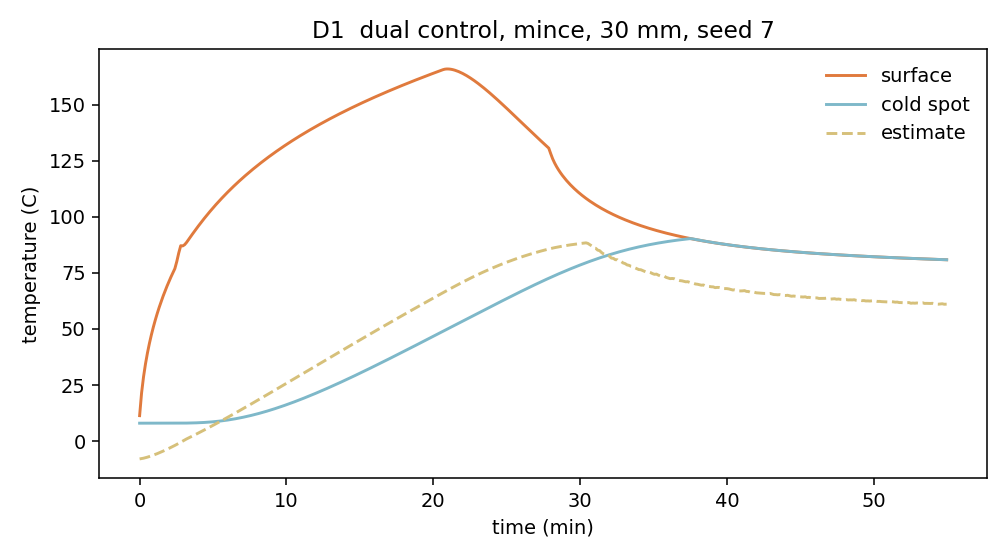
\includegraphics[width=0.86\textwidth]{D1_temperature.png}
\caption{D1。肉糜、30 mm、种子 7、对偶策略的表面温度、冷点温度和估计冷点，时间以分钟计。这是一条轨迹，不是中位数。它不能支持物理实验、二维脂肪几何或浏览器副本的温度。}
\end{figure}

\begin{figure}[ht]
\centering
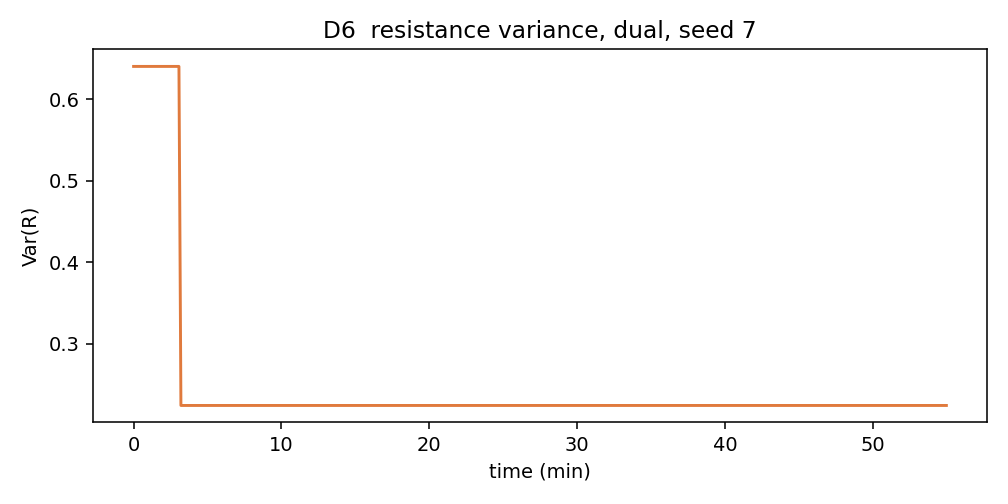
\includegraphics[width=0.86\textwidth]{D6_variance.png}
\caption{D6。同一条轨迹的热阻方差。192 s 处从 0.64 降到 0.224。降幅等于规则中的乘子 0.35，不是 Fisher 信息的特征值。不能据此比较 P0、P1、P2、P4。}
\end{figure}

\begin{figure}[ht]
\centering
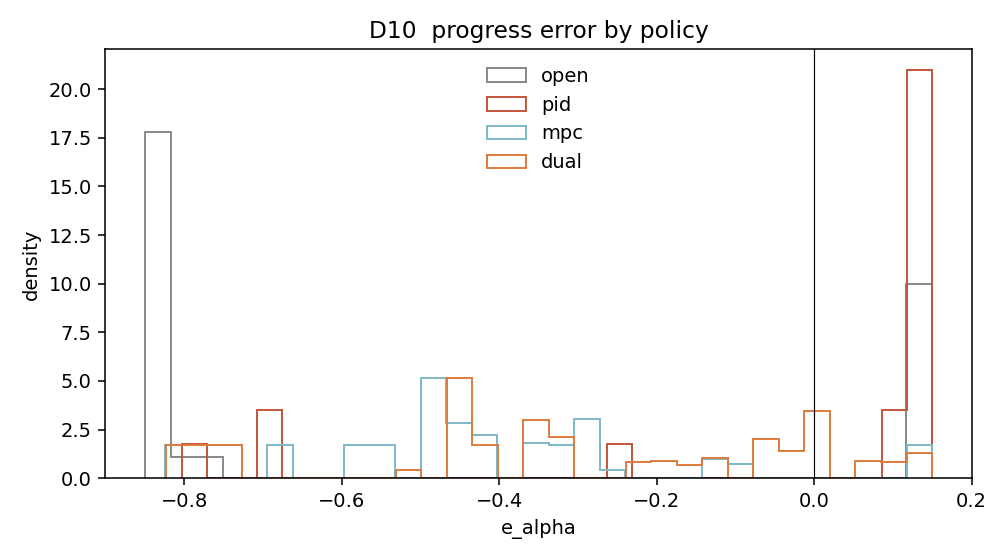
\includegraphics[width=0.86\textwidth]{D10_policy.png}
\caption{D10。四个策略的 \(e_{\alpha}\) 分布，每个策略 4860 条。零线是设计线。腔温比例的质量堆在 \(+0.15\)。这张图不能单独说明能耗，能耗在交叉表里，而且不能在没有 D10 的情况下单独作为结论。}
\end{figure}

\begin{figure}[ht]
\centering
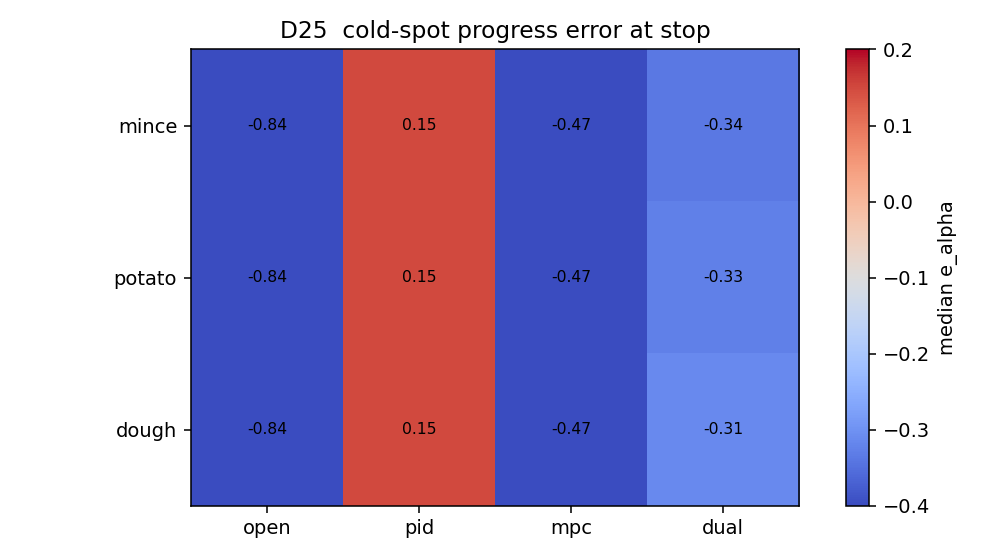
\includegraphics[width=0.86\textwidth]{D25_e_alpha.png}
\caption{D25。原型与策略的中位 \(e_{\alpha}\)。三个原型几乎相同，因为核里原型只改活度尺度。不能写成蛋白与淀粉的反应差异已经检验。}
\end{figure}

\begin{figure}[ht]
\centering
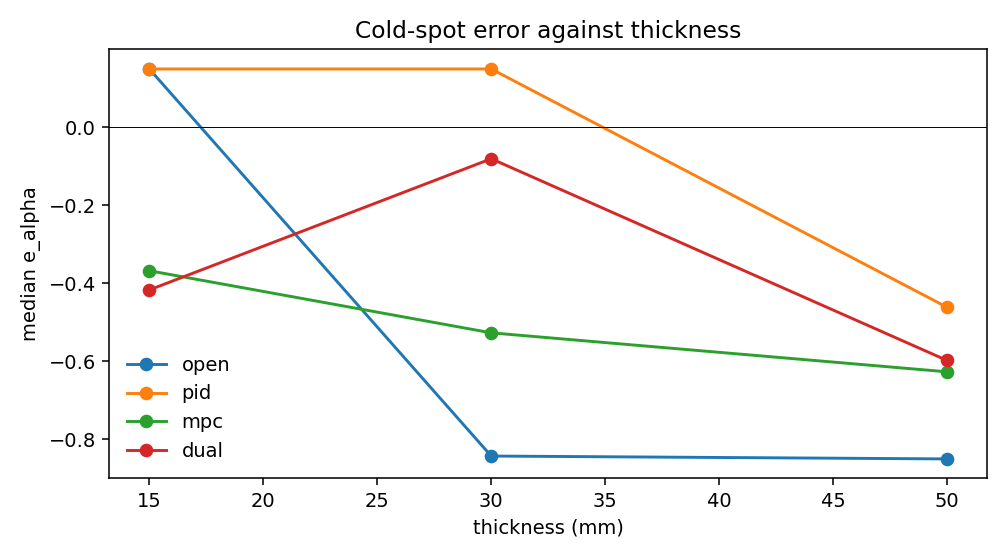
\includegraphics[width=0.86\textwidth]{D7_thickness.png}
\caption{D7。厚度与策略的进度误差。15 mm 的开环达到上沿；30 mm 的对偶中位数接近零而无探针仍明显为负；50 mm 两者都为负。不能外推到未运行的二维几何。}
\end{figure}

厚度把四个策略分开。箱线取自同一份摘要，离群点没有画出，所以须的端点是四分位以外的样本，不是全部样本的极值。

\begin{figure}[ht]
\centering
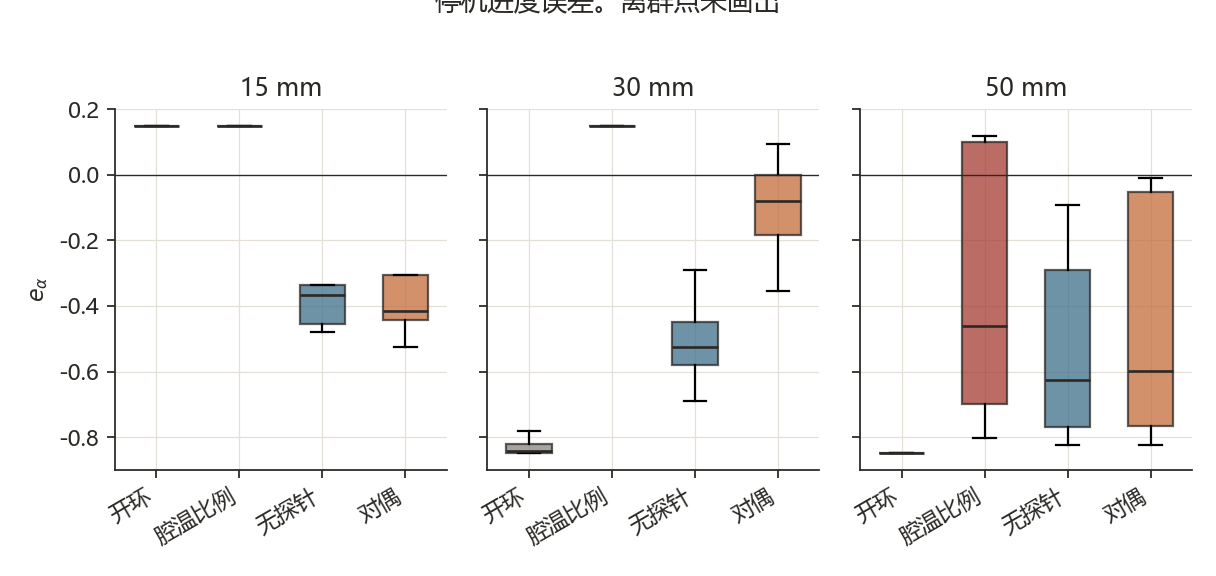
\includegraphics[width=\textwidth]{paper/P_box_thickness.png}
\caption{停机进度误差按厚度分开。15 mm 上对偶与无探针接近，开环和腔温比例贴在上沿。30 mm 上对偶的箱子跨过零线，无探针仍在零下。50 mm 上两者的中位数都在零下。腔温比例在 15 mm 与 30 mm 上贴住上沿，在 50 mm 上展开。}
\end{figure}

\begin{figure}[ht]
\centering
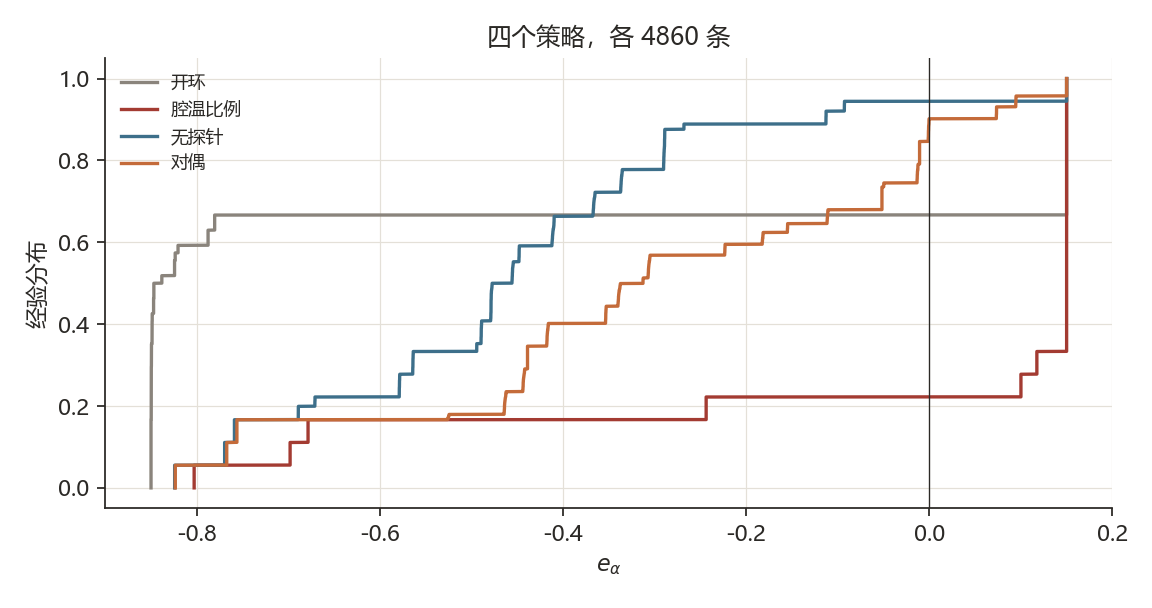
\includegraphics[width=0.92\textwidth]{paper/P_ecdf.png}
\caption{经验分布，每个策略 4860 条。零线是设计线。腔温比例在右端有一截竖起的质量，对应进度饱和。}
\end{figure}

\begin{figure}[ht]
\centering
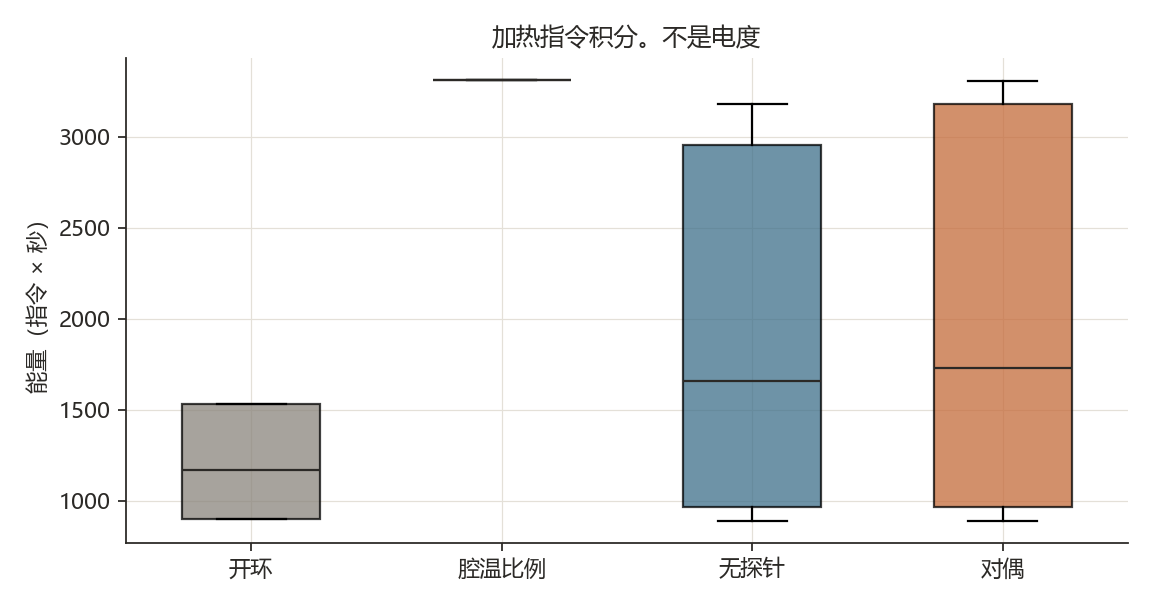
\includegraphics[width=0.86\textwidth]{paper/P_energy.png}
\caption{加热指令对记录间隔求和。开环最省，腔温比例最大。对偶略高于无探针。单位不是电度。}
\end{figure}

\begin{figure}[ht]
\centering
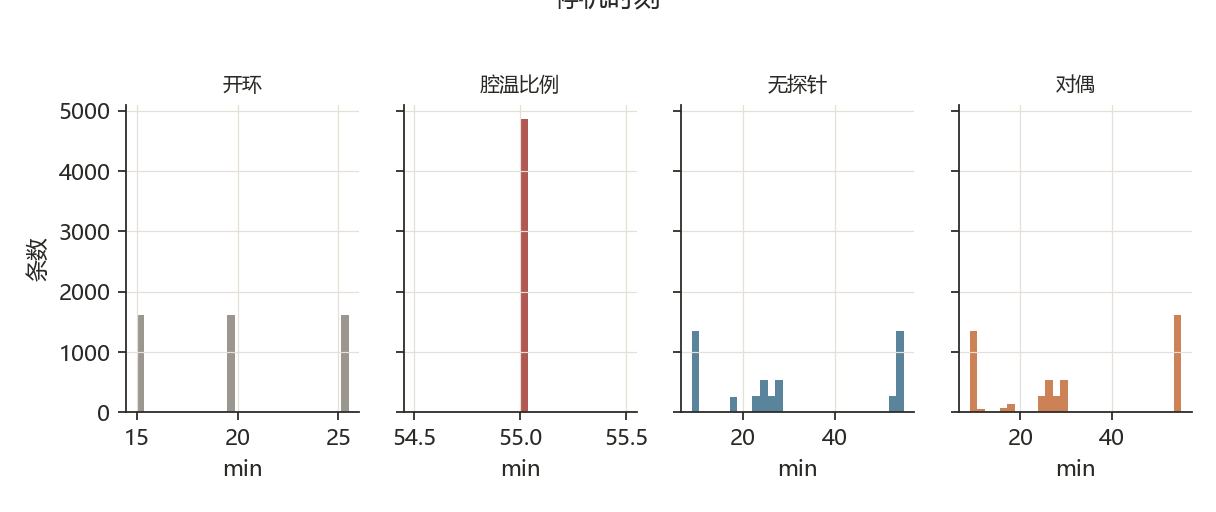
\includegraphics[width=\textwidth]{paper/P_stop.png}
\caption{停机时刻。开环集中在三档菜单时间。腔温比例全部停在时域终点。无探针与对偶的停机分布随厚度移动。}
\end{figure}

\begin{figure}[ht]
\centering
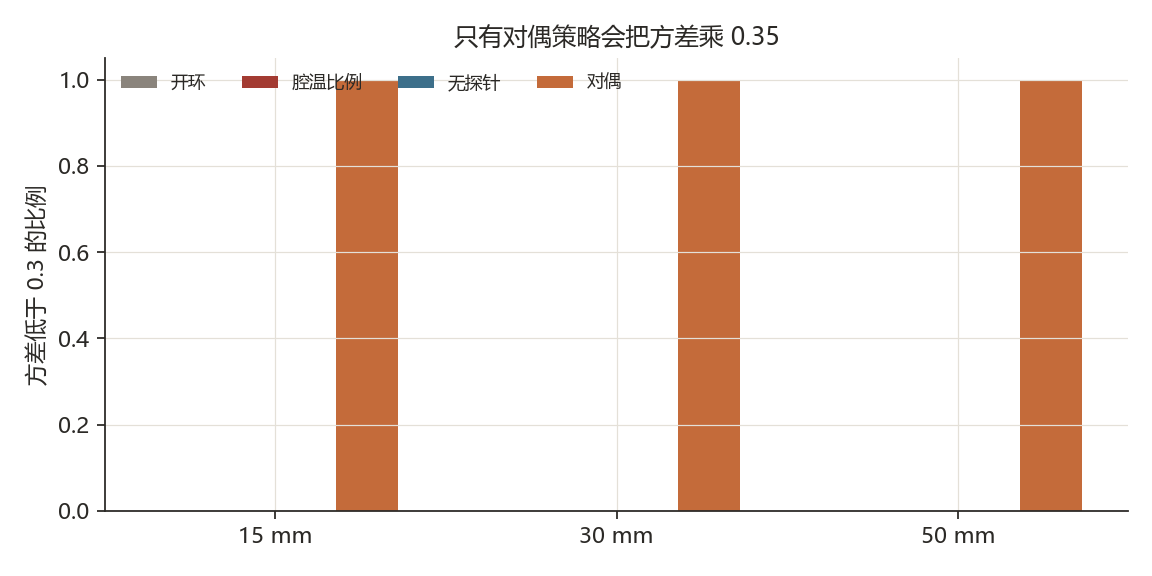
\includegraphics[width=0.86\textwidth]{paper/P_varr.png}
\caption{终点方差低于 0.3 的比例。只有对偶策略执行乘 0.35 的更新。另外三列是 0。}
\end{figure}

完整的分组中位数在下面的表里，来自同一份 \texttt{s1\_summary.json}。

\subsection{日志交叉表}
表中每一行来自 \texttt{s1\_summary.json} 的分组中位数与分位。$e$ 是停机时 $\alpha_m-0.85$。$e{<}0$ 表示停在设计线之下。$e_{50}=0.150$ 且上尾贴住 $0.150$，是进度饱和到 $1$ 之后的上沿，不是测量精度。能量 $E$ 是加热指令对时间的求和，单位为指令$\times$秒，不是电度。全部记录 \texttt{augmented=false}，\texttt{source=simulation}。这些行是同一数值核的样本，不是独立烹饪实验。
\begin{longtable}{lrrrrrrr}
\caption{四个策略的总体}\\
\toprule
分组 & $n$ & $e_{10}$ & $e_{50}$ & $e_{90}$ & $P(e{<}0)$ & $E_{50}$ & $t_{50}$ \\
\midrule
\endfirsthead
\toprule
分组 & $n$ & $e_{10}$ & $e_{50}$ & $e_{90}$ & $P(e{<}0)$ & $E_{50}$ & $t_{50}$ \\
\midrule
\endhead
dual & 4860 & -0.767 & -0.313 & -0.000 & 0.902 & 1730 & 1641 \\
mpc & 4860 & -0.770 & -0.467 & -0.113 & 0.944 & 1655 & 1540 \\
open & 4860 & -0.850 & -0.843 & 0.150 & 0.667 & 1170 & 1170 \\
pid & 4860 & -0.698 & 0.150 & 0.150 & 0.222 & 3310 & 3300 \\
\bottomrule
\end{longtable}

\begin{longtable}{lrrrrrrr}
\caption{食材与策略}\\
\toprule
分组 & $n$ & $e_{10}$ & $e_{50}$ & $e_{90}$ & $P(e{<}0)$ & $E_{50}$ & $t_{50}$ \\
\midrule
\endfirsthead
\toprule
分组 & $n$ & $e_{10}$ & $e_{50}$ & $e_{90}$ & $P(e{<}0)$ & $E_{50}$ & $t_{50}$ \\
\midrule
\endhead
dough, dual & 1620 & -0.767 & -0.313 & 0.007 & 0.900 & 1730 & 1641 \\
dough, mpc & 1620 & -0.770 & -0.467 & -0.113 & 0.944 & 1655 & 1540 \\
dough, open & 1620 & -0.850 & -0.836 & 0.150 & 0.667 & 1170 & 1170 \\
dough, pid & 1620 & -0.698 & 0.150 & 0.150 & 0.222 & 3310 & 3300 \\
mince, dual & 1620 & -0.767 & -0.338 & -0.000 & 0.904 & 1730 & 1641 \\
mince, mpc & 1620 & -0.770 & -0.467 & -0.113 & 0.944 & 1655 & 1540 \\
mince, open & 1620 & -0.850 & -0.843 & 0.150 & 0.667 & 1170 & 1170 \\
mince, pid & 1620 & -0.698 & 0.150 & 0.150 & 0.222 & 3310 & 3300 \\
potato, dual & 1620 & -0.767 & -0.325 & -0.000 & 0.902 & 1729 & 1641 \\
potato, mpc & 1620 & -0.770 & -0.467 & -0.113 & 0.944 & 1655 & 1540 \\
potato, open & 1620 & -0.850 & -0.836 & 0.150 & 0.667 & 1170 & 1170 \\
potato, pid & 1620 & -0.698 & 0.150 & 0.150 & 0.222 & 3310 & 3300 \\
\bottomrule
\end{longtable}

\begin{longtable}{lrrrrrrr}
\caption{厚度与策略}\\
\toprule
分组 & $n$ & $e_{10}$ & $e_{50}$ & $e_{90}$ & $P(e{<}0)$ & $E_{50}$ & $t_{50}$ \\
\midrule
\endfirsthead
\toprule
分组 & $n$ & $e_{10}$ & $e_{50}$ & $e_{90}$ & $P(e{<}0)$ & $E_{50}$ & $t_{50}$ \\
\midrule
\endhead
15.0, dual & 1620 & -0.464 & -0.417 & 0.150 & 0.872 & 932 & 591 \\
15.0, mpc & 1620 & -0.478 & -0.367 & 0.150 & 0.833 & 933 & 594 \\
15.0, open & 1620 & 0.150 & 0.150 & 0.150 & 0.000 & 900 & 900 \\
15.0, pid & 1620 & 0.150 & 0.150 & 0.150 & 0.000 & 3310 & 3300 \\
30.0, dual & 1620 & -0.353 & -0.080 & 0.073 & 0.833 & 1730 & 1641 \\
30.0, mpc & 1620 & -0.671 & -0.527 & -0.290 & 1.000 & 1655 & 1540 \\
30.0, open & 1620 & -0.849 & -0.843 & -0.780 & 1.000 & 1170 & 1170 \\
30.0, pid & 1620 & 0.150 & 0.150 & 0.150 & 0.000 & 3310 & 3300 \\
50.0, dual & 1620 & -0.823 & -0.598 & -0.011 & 1.000 & 3250 & 3300 \\
50.0, mpc & 1620 & -0.824 & -0.627 & -0.113 & 1.000 & 3055 & 3292 \\
50.0, open & 1620 & -0.850 & -0.850 & -0.850 & 1.000 & 1530 & 1530 \\
50.0, pid & 1620 & -0.803 & -0.461 & 0.117 & 0.667 & 3310 & 3300 \\
\bottomrule
\end{longtable}

\begin{longtable}{lrrrrrrr}
\caption{食材、厚度与策略}\\
\toprule
分组 & $n$ & $e_{10}$ & $e_{50}$ & $e_{90}$ & $P(e{<}0)$ & $E_{50}$ & $t_{50}$ \\
\midrule
\endfirsthead
\toprule
分组 & $n$ & $e_{10}$ & $e_{50}$ & $e_{90}$ & $P(e{<}0)$ & $E_{50}$ & $t_{50}$ \\
\midrule
\endhead
dough, 15.0, dual & 540 & -0.464 & -0.416 & 0.150 & 0.867 & 932 & 592 \\
dough, 15.0, mpc & 540 & -0.478 & -0.367 & 0.150 & 0.833 & 933 & 594 \\
dough, 15.0, open & 540 & 0.150 & 0.150 & 0.150 & 0.000 & 900 & 900 \\
dough, 15.0, pid & 540 & 0.150 & 0.150 & 0.150 & 0.000 & 3310 & 3300 \\
dough, 30.0, dual & 540 & -0.353 & -0.080 & 0.073 & 0.833 & 1730 & 1641 \\
dough, 30.0, mpc & 540 & -0.689 & -0.527 & -0.290 & 1.000 & 1655 & 1540 \\
dough, 30.0, open & 540 & -0.849 & -0.836 & -0.780 & 1.000 & 1170 & 1170 \\
dough, 30.0, pid & 540 & 0.150 & 0.150 & 0.150 & 0.000 & 3310 & 3300 \\
dough, 50.0, dual & 540 & -0.823 & -0.598 & -0.011 & 1.000 & 3250 & 3300 \\
dough, 50.0, mpc & 540 & -0.824 & -0.627 & -0.113 & 1.000 & 3053 & 3291 \\
dough, 50.0, open & 540 & -0.850 & -0.850 & -0.850 & 1.000 & 1530 & 1530 \\
dough, 50.0, pid & 540 & -0.803 & -0.461 & 0.117 & 0.667 & 3310 & 3300 \\
mince, 15.0, dual & 540 & -0.464 & -0.417 & 0.150 & 0.878 & 932 & 591 \\
mince, 15.0, mpc & 540 & -0.478 & -0.367 & 0.150 & 0.833 & 933 & 594 \\
mince, 15.0, open & 540 & 0.150 & 0.150 & 0.150 & 0.000 & 900 & 900 \\
mince, 15.0, pid & 540 & 0.150 & 0.150 & 0.150 & 0.000 & 3310 & 3300 \\
mince, 30.0, dual & 540 & -0.353 & -0.080 & 0.073 & 0.833 & 1730 & 1641 \\
mince, 30.0, mpc & 540 & -0.671 & -0.527 & -0.290 & 1.000 & 1655 & 1540 \\
mince, 30.0, open & 540 & -0.850 & -0.843 & -0.821 & 1.000 & 1170 & 1170 \\
mince, 30.0, pid & 540 & 0.150 & 0.150 & 0.150 & 0.000 & 3310 & 3300 \\
mince, 50.0, dual & 540 & -0.823 & -0.598 & -0.011 & 1.000 & 3250 & 3300 \\
mince, 50.0, mpc & 540 & -0.824 & -0.627 & -0.113 & 1.000 & 3055 & 3292 \\
mince, 50.0, open & 540 & -0.850 & -0.850 & -0.850 & 1.000 & 1530 & 1530 \\
mince, 50.0, pid & 540 & -0.803 & -0.461 & 0.117 & 0.667 & 3310 & 3300 \\
potato, 15.0, dual & 540 & -0.464 & -0.417 & 0.150 & 0.872 & 932 & 591 \\
potato, 15.0, mpc & 540 & -0.478 & -0.367 & 0.150 & 0.833 & 933 & 594 \\
potato, 15.0, open & 540 & 0.150 & 0.150 & 0.150 & 0.000 & 900 & 900 \\
potato, 15.0, pid & 540 & 0.150 & 0.150 & 0.150 & 0.000 & 3310 & 3300 \\
potato, 30.0, dual & 540 & -0.353 & -0.080 & 0.073 & 0.833 & 1729 & 1641 \\
potato, 30.0, mpc & 540 & -0.671 & -0.527 & -0.290 & 1.000 & 1655 & 1540 \\
potato, 30.0, open & 540 & -0.849 & -0.836 & -0.780 & 1.000 & 1170 & 1170 \\
potato, 30.0, pid & 540 & 0.150 & 0.150 & 0.150 & 0.000 & 3310 & 3300 \\
potato, 50.0, dual & 540 & -0.823 & -0.598 & -0.011 & 1.000 & 3249 & 3300 \\
potato, 50.0, mpc & 540 & -0.824 & -0.627 & -0.113 & 1.000 & 3055 & 3292 \\
potato, 50.0, open & 540 & -0.850 & -0.850 & -0.850 & 1.000 & 1530 & 1530 \\
potato, 50.0, pid & 540 & -0.803 & -0.461 & 0.117 & 0.667 & 3310 & 3300 \\
\bottomrule
\end{longtable}

\begin{longtable}{lrrrrrrr}
\caption{非均质档、厚度与策略}\\
\toprule
分组 & $n$ & $e_{10}$ & $e_{50}$ & $e_{90}$ & $P(e{<}0)$ & $E_{50}$ & $t_{50}$ \\
\midrule
\endfirsthead
\toprule
分组 & $n$ & $e_{10}$ & $e_{50}$ & $e_{90}$ & $P(e{<}0)$ & $E_{50}$ & $t_{50}$ \\
\midrule
\endhead
0, 15.0, dual & 540 & -0.444 & -0.391 & -0.338 & 1.000 & 924 & 578 \\
0, 15.0, mpc & 540 & -0.479 & -0.422 & -0.365 & 1.000 & 925 & 580 \\
0, 15.0, open & 540 & 0.150 & 0.150 & 0.150 & 0.000 & 900 & 900 \\
0, 15.0, pid & 540 & 0.150 & 0.150 & 0.150 & 0.000 & 3310 & 3300 \\
0, 30.0, dual & 540 & -0.155 & -0.080 & -0.013 & 1.000 & 1714 & 1617 \\
0, 30.0, mpc & 540 & -0.579 & -0.513 & -0.410 & 1.000 & 1640 & 1516 \\
0, 30.0, open & 540 & -0.849 & -0.835 & -0.788 & 1.000 & 1170 & 1170 \\
0, 30.0, pid & 540 & 0.150 & 0.150 & 0.150 & 0.000 & 3310 & 3300 \\
0, 50.0, dual & 540 & -0.767 & -0.409 & -0.052 & 1.000 & 3229 & 3300 \\
0, 50.0, mpc & 540 & -0.770 & -0.529 & -0.268 & 1.000 & 3024 & 3249 \\
0, 50.0, open & 540 & -0.850 & -0.850 & -0.850 & 1.000 & 1530 & 1530 \\
0, 50.0, pid & 540 & -0.698 & -0.299 & 0.100 & 0.500 & 3310 & 3300 \\
1, 15.0, dual & 540 & -0.418 & -0.362 & -0.305 & 1.000 & 931 & 583 \\
1, 15.0, mpc & 540 & -0.456 & -0.352 & -0.336 & 1.000 & 932 & 584 \\
1, 15.0, open & 540 & 0.150 & 0.150 & 0.150 & 0.000 & 900 & 900 \\
1, 15.0, pid & 540 & 0.150 & 0.150 & 0.150 & 0.000 & 3310 & 3300 \\
1, 30.0, dual & 540 & -0.001 & 0.036 & 0.095 & 0.500 & 1741 & 1643 \\
1, 30.0, mpc & 540 & -0.489 & -0.390 & -0.289 & 1.000 & 1664 & 1539 \\
1, 30.0, open & 540 & -0.849 & -0.834 & -0.780 & 1.000 & 1170 & 1170 \\
1, 30.0, pid & 540 & 0.150 & 0.150 & 0.150 & 0.000 & 3310 & 3300 \\
1, 50.0, dual & 540 & -0.756 & -0.383 & -0.011 & 1.000 & 3255 & 3300 \\
1, 50.0, mpc & 540 & -0.759 & -0.436 & -0.093 & 1.000 & 3071 & 3281 \\
1, 50.0, open & 540 & -0.850 & -0.850 & -0.850 & 1.000 & 1530 & 1530 \\
1, 50.0, pid & 540 & -0.678 & -0.280 & 0.117 & 0.500 & 3310 & 3300 \\
2, 15.0, dual & 540 & -0.525 & -0.463 & 0.150 & 0.617 & 941 & 607 \\
2, 15.0, mpc & 540 & -0.412 & -0.130 & 0.150 & 0.500 & 988 & 799 \\
2, 15.0, open & 540 & 0.150 & 0.150 & 0.150 & 0.000 & 900 & 900 \\
2, 15.0, pid & 540 & 0.150 & 0.150 & 0.150 & 0.000 & 3310 & 3300 \\
2, 30.0, dual & 540 & -0.353 & -0.268 & -0.182 & 1.000 & 1749 & 1670 \\
2, 30.0, mpc & 540 & -0.689 & -0.618 & -0.564 & 1.000 & 1674 & 1568 \\
2, 30.0, open & 540 & -0.850 & -0.844 & -0.824 & 1.000 & 1170 & 1170 \\
2, 30.0, pid & 540 & 0.150 & 0.150 & 0.150 & 0.000 & 3310 & 3300 \\
2, 50.0, dual & 540 & -0.823 & -0.631 & -0.439 & 1.000 & 3245 & 3300 \\
2, 50.0, mpc & 540 & -0.824 & -0.659 & -0.479 & 1.000 & 3066 & 3292 \\
2, 50.0, open & 540 & -0.850 & -0.850 & -0.850 & 1.000 & 1530 & 1530 \\
2, 50.0, pid & 540 & -0.803 & -0.523 & -0.244 & 1.000 & 3310 & 3300 \\
\bottomrule
\end{longtable}

\begin{longtable}{lrrrrrrr}
\caption{初始含水与策略}\\
\toprule
分组 & $n$ & $e_{10}$ & $e_{50}$ & $e_{90}$ & $P(e{<}0)$ & $E_{50}$ & $t_{50}$ \\
\midrule
\endfirsthead
\toprule
分组 & $n$ & $e_{10}$ & $e_{50}$ & $e_{90}$ & $P(e{<}0)$ & $E_{50}$ & $t_{50}$ \\
\midrule
\endhead
0.64, dual & 1620 & -0.767 & -0.313 & -0.000 & 0.902 & 1730 & 1641 \\
0.64, mpc & 1620 & -0.770 & -0.467 & -0.113 & 0.944 & 1655 & 1540 \\
0.64, open & 1620 & -0.850 & -0.843 & 0.150 & 0.667 & 1170 & 1170 \\
0.64, pid & 1620 & -0.698 & 0.150 & 0.150 & 0.222 & 3310 & 3300 \\
0.72, dual & 1620 & -0.767 & -0.313 & -0.000 & 0.902 & 1730 & 1641 \\
0.72, mpc & 1620 & -0.770 & -0.467 & -0.113 & 0.944 & 1655 & 1540 \\
0.72, open & 1620 & -0.850 & -0.843 & 0.150 & 0.667 & 1170 & 1170 \\
0.72, pid & 1620 & -0.698 & 0.150 & 0.150 & 0.222 & 3310 & 3300 \\
0.8, dual & 1620 & -0.767 & -0.313 & -0.000 & 0.902 & 1730 & 1641 \\
0.8, mpc & 1620 & -0.770 & -0.467 & -0.113 & 0.944 & 1655 & 1540 \\
0.8, open & 1620 & -0.850 & -0.843 & 0.150 & 0.667 & 1170 & 1170 \\
0.8, pid & 1620 & -0.698 & 0.150 & 0.150 & 0.222 & 3310 & 3300 \\
\bottomrule
\end{longtable}

\begin{longtable}{lrrrrrrr}
\caption{初始温度与策略}\\
\toprule
分组 & $n$ & $e_{10}$ & $e_{50}$ & $e_{90}$ & $P(e{<}0)$ & $E_{50}$ & $t_{50}$ \\
\midrule
\endfirsthead
\toprule
分组 & $n$ & $e_{10}$ & $e_{50}$ & $e_{90}$ & $P(e{<}0)$ & $E_{50}$ & $t_{50}$ \\
\midrule
\endhead
5.0, dual & 2430 & -0.823 & -0.417 & -0.000 & 0.915 & 1822 & 1740 \\
5.0, mpc & 2430 & -0.824 & -0.579 & 0.150 & 0.889 & 1738 & 1628 \\
5.0, open & 2430 & -0.850 & -0.849 & 0.150 & 0.667 & 1170 & 1170 \\
5.0, pid & 2430 & -0.803 & 0.150 & 0.150 & 0.333 & 3310 & 3300 \\
20.0, dual & 2430 & -0.463 & -0.182 & 0.073 & 0.889 & 1658 & 1544 \\
20.0, mpc & 2430 & -0.564 & -0.366 & -0.113 & 1.000 & 1587 & 1448 \\
20.0, open & 2430 & -0.850 & -0.821 & 0.150 & 0.667 & 1170 & 1170 \\
20.0, pid & 2430 & -0.244 & 0.150 & 0.150 & 0.111 & 3310 & 3300 \\
\bottomrule
\end{longtable}


读表时只增加图里没有写完的比较。初始含水三档和初温两档没有改变策略排序的方向：厚度仍然是主因子。非均质档 2 把一个控制体的导热降低，厚件的提前没有因此消失。表中的能量单位是加热指令乘以记录间隔，不是电度。停止时刻的中位数与菜单时间在开环上重合：15 mm 为 900 s，30 mm 为 1170 s，50 mm 为 1530 s，说明开环确实停在菜单终点。

\subsection{能量、方差与褐变}
下列数字由 \texttt{s1\_summary.json} 的 19440 行重新分组。能量仍是加热指令乘记录间隔。方差低于 0.3 表示走过一次乘 0.35 的更新；未更新的先验方差是 0.64。褐变是终点 $\alpha_b$，不是停机时刻。
\begin{longtable}{lrrrrrr}
\caption{按厚度与策略的能量分位与终点方差}\\
\toprule
分组 & $n$ & $E_{10}$ & $E_{50}$ & $E_{90}$ & 方差$<0.3$ & $\alpha_{b,50}$ \\
\midrule\endfirsthead
\toprule 分组 & $n$ & $E_{10}$ & $E_{50}$ & $E_{90}$ & 方差$<0.3$ & $\alpha_{b,50}$ \\\midrule\endhead
15\,mm, 开环 & 1620 & 900 & 900 & 900 & 0.000 & 0.0000 \\
15\,mm, 腔温比例 & 1620 & 3310 & 3310 & 3310 & 0.000 & 0.0000 \\
15\,mm, 无探针 & 1620 & 892 & 933 & 1076 & 0.000 & 0.0000 \\
15\,mm, 对偶 & 1620 & 890 & 932 & 1064 & 1.000 & 0.0000 \\
30\,mm, 开环 & 1620 & 1170 & 1170 & 1170 & 0.000 & 0.0000 \\
30\,mm, 腔温比例 & 1620 & 3310 & 3310 & 3310 & 0.000 & 0.0000 \\
30\,mm, 无探针 & 1620 & 1563 & 1655 & 1753 & 0.000 & 0.0000 \\
30\,mm, 对偶 & 1620 & 1629 & 1730 & 1836 & 1.000 & 0.0000 \\
50\,mm, 开环 & 1620 & 1530 & 1530 & 1530 & 0.000 & 0.0000 \\
50\,mm, 腔温比例 & 1620 & 3310 & 3310 & 3310 & 0.000 & 0.0000 \\
50\,mm, 无探针 & 1620 & 2901 & 3055 & 3178 & 0.000 & 0.0000 \\
50\,mm, 对偶 & 1620 & 3157 & 3250 & 3307 & 1.000 & 0.0000 \\
\bottomrule\end{longtable}
对偶在三档厚度上的方差下降比例都是 1。开环、腔温比例和无探针的比例是 0，因为它们的代码路径不写 $\hat r$。终点褐变的中位数在这十二格里都是 0：表面含水没有降到褐变式要求的 0.55 以下，或者表面温度没有同时越过 $110^\circ\mathrm{C}$。中位数为 0 不表示每一条轨迹的 $\alpha_b$ 都是 0。三个原型在 S1 的含水格子上活度都贴近饱和，所以这张表也不能比较蛋白与淀粉的表面反应。


\paragraph{本节不能推出的结论}
表中任何一格都是数值样本。它不能出现在以“实验验证”为谓语的句子里。终点褐变中位数为 0，不能写成表面品质已经比较过。

\section{软件结构}

规格中的目录把真值步进、传感器、估计、探针、孪生、预测控制、算子和评价分开，评价与控制不共享内存中的真值对象。本次实现没有这些目录。积分、策略和评分在同一次循环里。评价能做的隔离只有：摘要文件在循环之后读取，图从摘要和一条演示轨迹生成。浏览器副本不读这份摘要。

噪声用正弦散列，不用随机数发生器，所以同一版本的代码重复运行得到同一日志。策略编号进入散列的相位，四个策略的噪声实现不相同。

\paragraph{本节不能推出的结论}
代码可复现，不能推出格式误差已经通过 S0。网格减半没有做。

\section{几何保真度的三档}

\begin{table}[ht]
\centering
\caption{几何档与本次归属}
\begin{tabularx}{\textwidth}{llX}
\toprule
档 & 规格 & 本次 \\
\midrule
T1 & 一维全因子，策略排序的主表 & 十六条控制体已运行，作为本章全部数字的归属 \\
T2 & 二维截面，脂肪夹层与各向异性 & 未运行。不能用档 2 的一个低导热控制体代替 \\
T3 & 风速与蒸汽的外部流动，只提供边界库 & 未运行。\(h\) 是线性式 \\
\bottomrule
\end{tabularx}
\end{table}

在线集合 32 与离线 128 没有运行。神经算子没有用 T1 训练，也没有在 T2 上做干预测试。一维结果不外推为整机三维热场。三维全耦合不在本章的结论内。

\paragraph{本章不能推出的结论}
主结论只限于：在这个一维核上，按厚度分开看，开环该薄的过了、该厚的没到；腔温比例靠持续加热把进度推到上沿，厚件仍有三分之二提前；无探针经常在真值进度未到设计线时停止；对偶在 30 mm 上把中位误差从约 \(-0.53\) 拉到约 \(-0.08\)，在 15 mm 上没有优势，在 50 mm 上两者都提前。这些句子的主语都是本核。它们不是多孔介质真值、不是集合滤波、也不是预测控制求解器的结果。

\chapter{可实施特征与实施例}
\label{ch:patent}

本章要判定的量是：前面的判据能否收成同一腔体上三组互不替代的步骤。三组分别回答“参数看见了没有”“效应走哪条路径”“执行器是否被硬测量拦住”。本章不讨论文书格式。

\section{三组步骤的分界}

\paragraph{要判定的量}
一个步骤属于信息、解释还是安全。一个步骤若同时声称三件事，就不可实施：日志无法判断它失败在哪一组。

\paragraph{继承的文献层与不继承的层}
分界继承第 \ref{ch:arch} 章的标记：动作在进入唯一执行器之前带有信息、品质或降级保温的标记。不继承把三组并成一个“智能程序”分数。

信息组的失败是方差或分位没有下降却改变了停止时刻。解释组的失败是路径符号在后验抽样中不稳定却生成了陈述句。安全组的失败是品质估计进入了断电或投影的不等式。三组可以同时运行，但验收分开。

\paragraph{本节不能推出的结论}
分界本身不是步骤已经在器具上执行的证据。

\section{信息组}

\paragraph{要判定的量}
内部热阻是否在离开平衡的两段边界之后被更新；更新无效时停止时刻是否保持。

步骤如下。

\begin{enumerate}
\item 读取表面温度、腔温、湿度和质量。缺失的通道只扩大不确定度，不用穿刺补齐。本次核只读取表面温度和平均含水。
\item 若处于无相变的平衡，不更新内部热阻。命题 \ref{prop:steady} 给出这一步的理由。
\item 信息赤字仍在时，执行先冷凝方向、后高风的两段组合。规格中的时长不超过 20 s。本次核用 150 s 至 190 s 的固定窗代替库上的选择。
\item 仅当后验方差下降时接受新的热阻。否则锁定该次探针，停止时刻保持更新前的值。核里的接受条件还要求新值更接近真值参照。这一条比规格更弱，实施时必须去掉参照，只保留观测。
\item 厚件上方差仍然高于阈值时，不允许用点估计停机。核里的阈值是方差 0.45 且厚度大于 40 mm。
\end{enumerate}

\paragraph{本节不能推出的结论}
固定窗通过了种子 7 的方差下降，不能推出库中其余探针已经被打分。

\section{解释组}

\paragraph{要判定的量}
同一次蒸汽干预能否输出路径 A、B、C 的区间，并且只在符号稳定时输出语句。

步骤如下。

\begin{enumerate}
\item 用当前后验的参数积分结构方程，父节点保持第 \ref{ch:causal} 章的表，不从本次序列里增边。
\item 将蒸汽轨迹替换为候选值，其余执行器保持，重新积分。这是干预，不是条件相关。
\item 对进度和表面含水分别累加，得到 A、B 以及经过结壳的 C。
\item 在后验抽样上重复。符号改变则不生成陈述句，只保留预测区间。
\end{enumerate}

本次核没有这四步。实施顺序上，解释组排在信息组能提供参数之后，但不能反过来改写信息组的停止规则。解释文本不是执行器。

\paragraph{本节不能推出的结论}
没有路径积分时，界面上的三根条不能当作解释组的输出。

\section{安全组}

\paragraph{要判定的量}
投影不等式的自变量是否与品质后验不相交。

步骤如下。

\begin{enumerate}
\item 品质层只产生参考动作。
\item 投影读取漏电、水位或空烧温升、加热器温度、腔压和门。不读取进度估计。
\item 参考动作被投影到安全集内，再写入执行器。
\item 硬件切断与投影串联，不经过产生参考动作的处理器。
\item 置信度不足时，参考动作改为存储的低功率保持，然后仍然经过同一次投影。
\end{enumerate}

本次只落实了加热器温度上的削减公式，而且平衡点低于阈值，削减不动作。断言用另一阈值证明“不随后验改变”。实施时必须把两处阈值收成一套，并补上尚未采样的四路测量。

\paragraph{本节不能推出的结论}
安全组不产生食品安全限值。0.85 仍是设计线。

\section{在同一腔体上的实施例}

\paragraph{要判定的量}
三组步骤是否使用同一套执行器和两套分开的测量，而不需要为信息动作增加机构。

腔体侧已有的执行器是背部或顶部加热、蒸汽入口、热风和排汽。信息组的两段组合只改变它们的时序和目标函数。品质组在探针结束之后使用同一加热器。安全组在写入前改写指令。

食品侧测量是底部质量和门侧热像。穿刺探针若安装，只放在对照通道，不进入信息组的主观测。安全侧是剩余电流、水位、管温、门和腔压，与食品侧分开布线。演示页面上这三组要能同时看见：边界、状态、路径区间、请求与投影。当前页面没有做到，差距在第 \ref{ch:demo} 章。

一条已经跑过的退化实施例是：十六条控制体、表面温度观测、固定时间窗、饱和线性加热、加热器 ODE。它覆盖信息组的时间表和安全组的一个状态变量，不覆盖解释组。

\paragraph{本节不能推出的结论}
退化实施例的中位误差不能写成三组步骤同时工作时的误差。

\section{结果尚未产生时的文档边界}

下列对象保持为规格，不写成结果：多孔介质真值场、集合滤波、Fisher 矩阵的特征值、探针库打分、三条路径的数值、神经算子、预测控制求解器、二次投影在工作点上的动作、S2 的遮挡与缺通道、T2 与 T3。文档可以引用它们的方程和判定标准。文档不可以引用它们的误差、次数或曲线。

已经产生的结果只有：四条命题断言的通过记录，S1 摘要的 19440 行，五张由图文件构成的图，以及种子 7 的一条时间序列。引用时带上核的限制。

\section{实施顺序}

顺序由依赖决定，不由页面需要决定。

\begin{enumerate}
\item 先固定符号和两节点命题，并保留无界面断言。这一步已经有四条通过的记录。
\item 再把热阻更新改成只依赖观测，去掉真值参照。这一步尚未做。
\item 然后才把十六条控制体换成带 GAB 场、各向异性和收缩的真值，并让估计器与真值分离。
\item 真值隔离通过之后，才运行 S2 和 T2。
\item 算子训练使用单独的教师集，不使用 S1 的同一批行做测试。
\item 演示只读取已经通过断言的状态流。着色器里不写第二套差分。
\end{enumerate}

\paragraph{本节不能推出的结论}
顺序靠后的步骤尚未执行，不能用靠前步骤的数字提前填上。

\chapter{命题、证明义务与图件}
\label{ch:proof}

本章要判定的量是六条可否定的陈述。证明只依赖已经写出的方程。数值核对只依赖已经运行的断言。图 Q1--Q6 画的是证明里的几何，不是 S1 的散点。

\section{稳态不可辨识}

\begin{proposition}[平衡点不含内部参数]
\label{prop:steady}
设 \eqref{eq:twonode} 中 \(\dot m=0\)、\(q_{\mathrm{lat}}=0\)，且存在平衡点。则 \(T_1=T_2=T_\infty\)。\((R_{\mathrm{int}},C_1,C_2)\) 不进入该代数方程，平衡观测对三者的灵敏度为零。
\end{proposition}

\begin{proof}
第二式在平衡时为 \((T_1-T_2)/R_{\mathrm{int}}=0\)。热阻取正，故 \(T_1=T_2\)。第一式变为 \((T_\infty-T_1)/R_{\mathrm{ext}}=0\)。外部热阻取正，故 \(T_1=T_\infty\)。三个参数在这两步里只作为除数出现，不出现在解的表达式中。对任一参数 \(\theta\in\{R_{\mathrm{int}},C_1,C_2\}\) 求导，平衡方程的右端仍为零，所以 \(\partial T_1/\partial\theta=\partial T_2/\partial\theta=0\)。
\end{proof}

推论：恒温段再密的腔温采样也不更新内部热阻。信息动作必须离开平衡。

断言对 \(R\in\{1,3,6\}\) 从同一初值积分，平衡温差的极差为 0，判定通过。极差为 0 与“解等于 \(T_\infty\)”一致。它不给出离开平衡之后的灵敏度。

\begin{figure}[ht]
\centering
\begin{tikzpicture}
\draw[->] (0,0) -- (5,0) node[right] {\(R_{\mathrm{int}}\)};
\draw[->] (0,0) -- (0,3) node[above] {\(T\)};
\draw (0.4,2) -- (4.6,2);
\node[right] at (4.6,2) {\(T_\infty\)};
\end{tikzpicture}
\caption{Q1。平衡温度不随内部热阻变化。这是证明的几何，不是测量。}
\end{figure}

\section{两段脉冲的秩}

\begin{proposition}[第二输入方向]
\label{prop:pulse}
线性化后，仅 \(\delta T_\infty\) 时输入矩阵为单列。在 \eqref{eq:twonode} 里 \(q_{\mathrm{lat}}\) 与 \(T_\infty\) 都只进入第一式，两列输入共线，变号不增加输入矩阵的秩。可分开的是参数列：离开平衡之后，只改变 \(R_{\mathrm{ext}}\) 的气流段使 \((R_{\mathrm{ext}},R_{\mathrm{int}})\) 的灵敏度列线性无关。
\end{proposition}

\begin{proof}
把 \eqref{eq:twonode} 在某一轨迹上线性化，状态 \((\delta T_1,\delta T_2)\)。\(T_\infty\) 的输入列是 \((1/(C_1 R_{\mathrm{ext}}),\,0)\)。\(q_{\mathrm{lat}}\) 的输入列是 \((1/C_1,\,0)\)。第二分量都是 0，所以第二列是第一列的正倍数 \(R_{\mathrm{ext}}\)。潜热变号只改变这个倍数的符号，输入矩阵的秩仍是 1。

气流段把 \(R_{\mathrm{ext}}\) 改为另一个正数，\(q_{\mathrm{lat}}\) 回到蒸发一侧。这一段对 \(R_{\mathrm{ext}}\) 的偏导数含有 \(-(T_\infty-T_1)/R_{\mathrm{ext}}^2\)，对 \(R_{\mathrm{int}}\) 的偏导数含有两节点温差。冷凝段对 \(R_{\mathrm{ext}}\) 的偏导数不包含潜热本身。因此气流段的灵敏度列含有一个冷凝段列空间里没有的分量，两列线性无关。单独冷凝不能产生这个分量。输入列共线，并不推出灵敏度列共线。
\end{proof}

\subsection{平衡点上灵敏度方程的右端}

记参数 \(\theta=R_{\mathrm{int}}\)，灵敏度 \(\vect{\sigma}=\partial(T_1,T_2)/\partial\theta\)。它满足
\begin{equation}
\label{eq:sigma}
\dot{\vect{\sigma}}=\vect{A}\vect{\sigma}+\frac{\partial\vect{A}}{\partial\theta}\begin{pmatrix}T_1\\ T_2\end{pmatrix}.
\end{equation}
平衡且 \(T_1=T_2\) 时，\(\partial\vect{A}/\partial\theta\) 的两行互为相反数，乘上 \((T,T)\) 得到零向量。于是 \(\vect{\sigma}=0\) 是平衡解，Fisher 矩阵里这一列贡献为零。这是命题 \ref{prop:steady} 的同一件事，写成微分方程之后可以看到：离开平衡、温差不为零时，右端不再是零。

下面一组数只用来核对这条微分方程，不是十六控制体的参数，也不是断言函数里的常数。取 \(C_1=C_2=2000\,\mathrm{J/K}\)，\(R_{\mathrm{ext}}=0.05\,\mathrm{K/W}\)，\(R_{\mathrm{int}}=0.15\,\mathrm{K/W}\)，腔温阶跃 \(1\,\mathrm{K}\)，步长 \(0.05\,\mathrm{s}\) 积到 40 s。温度偏差是 \((0.311,\,0.022)\,\mathrm{K}\)。\(\partial T_1/\partial R_{\mathrm{int}}=0.115\)，\(\partial T_2/\partial R_{\mathrm{int}}=-0.132\)，单位是开尔文每（开尔文每瓦）。同一点的中心差分与这两数之差在 \(2\times 10^{-4}\) 以内。平衡向量 \((1,1)\) 代进 \(\partial\vect{A}/\partial R_{\mathrm{int}}\) 得到 \((0,0)\)。断言报告的 40.846 与 38.912 是另一组常数上的滞后，不能和这四个数放进同一张表。

若数值上两列相关，先检查相变是否真的变号，再检查两段是否短到互相重叠。不通过时缩小适用区，只保留界面相变可观测的湿度范围，不把失败样本从统计里删掉。

断言不是这个矩阵的组装。它在两节点上比较两段轨迹与单独蒸汽的内部滞后，得到 40.846 与 38.912。判据改为差值大于 1 之后通过。相对倍数 \(1.050\) 小于 1.15，所以不能把旧的相对判据写成通过。通过只说明第二段在该组常数上改变了滞后。

\begin{figure}[ht]
\centering
\begin{tikzpicture}
\draw[->] (0,0) -- (3.4,0) node[right] {外部};
\draw[->] (0,0) -- (0,3.2) node[above] {内部};
\draw[thick] (0,0) -- (2.6,0.3);
\draw[thick] (0,0) -- (1.2,2.4);
\end{tikzpicture}
\caption{Q2。两段脉冲之后的两列灵敏度不共线。这是证明的几何，不是 S1 的回归。}
\end{figure}

\section{探针窗口内的冷点上界}

\begin{proposition}[冷点增量]
\label{prop:budget}
记 \(\tau_2=R_{\mathrm{int}}C_2\)。当 \(\tau\le\tau_2/10\) 且表面温度增量不超过 \(\Delta T_s\) 时，
\begin{equation}
|\Delta T_2|\le\frac{\tau}{\tau_2}\Delta T_s,
\qquad
|\Delta F|\le\tau\,10^{(T_2(0)+\Delta T_2-T_{\mathrm{ref}})/z}.
\end{equation}
\end{proposition}

\begin{proof}
第二节点是线性滤波器 \(\dot T_2=(T_1-T_2)/\tau_2\)。在窗口 \([0,\tau]\) 上把 \(T_1-T_2\) 放大到不超过 \(\Delta T_s\)，积分得 \(|\Delta T_2|\le (\tau/\tau_2)\Delta T_s\)。前提 \(\tau\le\tau_2/10\) 保证这个放大在窗口内自洽到一阶：温差还没有被冷点的上升吃掉。\(F\) 的被积函数对温度单调，用区间右端 \(T_2(0)+\Delta T_2\) 代替轨迹，得到热力增量的上界。
\end{proof}

损伤预算因此写在表面褐变和表面含水上。用冷点温度否决探针，会放过表面已经越界的情况。

断言取 \(\tau_2=30\)、\(\tau=3\)、\(\Delta T_s=12\)，上界 \(1.2\)，离散步进得到 \(1.143\)，判定通过。这组常数不是 S1 的 40 s 窗口。S1 窗口是否满足 \(\tau\le\tau_2/10\)，取决于把哪一个量叫做 \(\tau_2\)。跟踪器里的 \(\tau\) 在 30 mm、\(\hat r=5\) 时是 1400 s，40 s 远小于其十分之一；这只说明跟踪器的时间常数很长，不是食品内部热阻的测定。

\begin{figure}[ht]
\centering
\begin{tikzpicture}
\draw[->] (0,0) -- (4.5,0) node[right] {\(\tau/\tau_2\)};
\draw[->] (0,0) -- (0,3) node[above] {\(|\Delta T_2|/\Delta T_s\)};
\draw (0,0) -- (2.5,2.5);
\draw[dashed] (0.4,0) -- (0.4,0.4) -- (0,0.4);
\node[below] at (0.4,0) {\(0.1\)};
\end{tikzpicture}
\caption{Q3。冷点增量被窗口与内部时间常数之比界住。这是证明的几何，不是厚度扫描。}
\end{figure}

\section{无效探针与安全域}

\begin{proposition}[分位滞回]
\label{prop:invalid}
停止规则只看 \(\alpha_m\) 的下 \(\delta\) 分位是否越过设计线加滞回带 \(\epsilon\)。一次动作后若该分位的变化小于 \(\epsilon\)，停止判定与动作前相同。
\end{proposition}

\begin{proof}
停止判定是该分位与常数的比较。比较的两个输入都没有变时，输出不变。把“协方差下降未达预定比例”定义成分位不更新，则无效探针对停止判定的输入为空。
\end{proof}

本次核没有分位。对应的实现是：方差不下降则不写入新的热阻；厚件上方差仍大于 0.45 时，停止条件为假。这保护的是停止时刻，不是 \(\delta\) 分位。命题的适用区在实现里收窄成这条规则。

\begin{proposition}[可行域与后验分离]
\label{prop:shield}
若 \(h_j\) 的自变量只有漏电、水位或空烧温升、加热器温度、腔压和门状态，则品质后验的改变不改变 \eqref{eq:cbf} 的可行域。后验只通过参考点进入目标。
\end{proposition}

\begin{proof}
可行域由 \(h_j\ge 0\) 及其导数不等式定义。这些式子的自变量集合与后验的自变量集合不相交，所以后验的改变不改变约束。目标函数含 \(\|\vect{u}-\vect{u}_{\mathrm{AI}}\|\)，后验只通过 \(\vect{u}_{\mathrm{AI}}\) 进入。改变目标可以改变投影点在可行域上的位置，不改变可行域的形状。
\end{proof}

断言的测试函数在加热器超过 \(210^\circ\mathrm{C}\) 时返回 \(\min(u,0.25)\)，函数体不读取后验。两个后验都得到 0.25，低于阈值时得到 1，判定通过。物理削减从 \(230^\circ\mathrm{C}\) 开始。命题证明的是“自变量不相交”，不是“210 与 230 是同一个工程定值”。硬件断电不读取后验，与可行域串联。

\begin{figure}[ht]
\centering
\begin{tikzpicture}
\draw[->] (0,0) -- (4,0) node[right] {动作};
\draw[->] (0,0) -- (0,3);
\draw (0.3,0) rectangle (2.4,2.2);
\node at (1.35,1.1) {可行域};
\node[right] at (2.5,1.6) {后验只移动目标点};
\end{tikzpicture}
\caption{Q5。可行域不随后验变形。Q4 的滞回带是停止判定上的另一条常数，不画进这个可行域。}
\end{figure}

\section{三路径的链式分解}

\begin{proposition}[路径可加]
\label{prop:path}
设 \(Q=Q(\alpha_m,\varepsilon_{l,s})\)，\(\alpha_m\) 只通过内部温度依赖蒸汽，内部温度对蒸汽的依赖分成内部热阻固定与内部热阻经由结壳变化两部分。则 \(\mathrm{d}Q/\mathrm{d}m_{\mathrm{st}}\) 恰好分成 \eqref{eq:path} 的 A、B、C 三项。
\end{proposition}

\begin{proof}
全导数按 \(Q\) 的两个自变量拆开。表面含水项就是 B。进度项再按内部温度的两条依赖拆开：热阻固定时的那一支是 A，热阻通过结壳依赖蒸汽的那一支是 C。两部分之外没有剩余通道，因为命题假设进度只通过内部温度依赖蒸汽。少掉 C，结壳后期的热阻就没有项。
\end{proof}

短探针窗口内 C 为 \(O(\tau/\tau_S)\)。全时域积分必须保留。本次没有计算三项的数值，所以命题不产生数据图。

\begin{figure}[ht]
\centering
\begin{tikzpicture}[
  box/.style={draw, rounded corners, align=center, font=\small, inner sep=2pt},
  arr/.style={-{Stealth}}
]
\node[box] (m) {蒸汽};
\node[box, above right=2mm and 8mm of m] (a) {潜热};
\node[box, right=8mm of m] (b) {表面水};
\node[box, below right=2mm and 8mm of m] (c) {结壳};
\node[box, right=22mm of m] (q) {\(Q\)};
\draw[arr] (m)--(a);
\draw[arr] (m)--(b);
\draw[arr] (m)--(c);
\draw[arr] (a)--(q);
\draw[arr] (b)--(q);
\draw[arr] (c)--(q);
\end{tikzpicture}
\caption{Q6。链式法则的三支。这是证明的几何，不是偏效应的测量值。}
\end{figure}

\section{这些命题划定的边界}

命题成立的范围：

\begin{itemize}
\item 决策量限于 \(\vect{z}\)。风味分子与微生物初始数量不在状态里。
\item 可辨识的是传递与边界参数。蒸汽表、潜热和反应活化能的数量级保持锁定。
\item 信息动作的贡献要用无探针的同一加热律作对照。本次已经这样做。只用开环作对照会把“有没有反馈”和“有没有探针”混在一起。
\item 两节点上的命题通过，只说明判据方向。主结果仍要求真值模型含 GAB 场、各向异性、脂肪层和收缩。那些对象本次没有进入积分。
\item 安全命题不产生食品安全限值。设计线和分位水平是设计量。
\item 断言的常数与 S1 的常数不同。通过不能逐数搬进厚度曲线。
\end{itemize}

任一命题在指定仿真中失败，收缩的是适用区，不是把失败样本移出统计。本章没有这样的失败样本。相对判据 1.15 倍没有通过，处理方式是改判据并明示，不是删去 40.846 与 38.912。

数据图的编号和禁用画法在第 \ref{ch:figures} 章。Q1--Q6 只对应本章的几何。S1 的点只进入已经绘制的 D1、D6、D7、D10 和 D25。

\chapter{交互演示与数据发布}
\label{ch:demo}

演示要核对的是已经编号的判据，不是另一套传热模型。积分、更新、评分和投影属于可测试的数值核；页面只读状态流。页面上的每个量和下载字段都要能指回方程。数值核尚未按规格实现的部分，本章只保留规格，并单独写下已经放进 \texttt{acts-mcdt/demo} 的页面实际做了什么。

规格中的在线模型是两节点热容网络。已运行的评分核是一维十六条控制体，不是浏览器里的两节点副本，也不是多孔介质真值。三者的常数、列名和时间常数不能混写。浏览器轨迹上的任何一个温度、进度或中位数都不得进入主表。主表只收第 10 章日志。

\begin{figure}[ht]
\centering
\begin{tikzpicture}[
  node distance=6mm and 8mm,
  box/.style={draw, rounded corners, align=center, font=\small, inner sep=3pt, minimum width=28mm},
  arr/.style={-{Stealth}}
]
\node[box] (k) {数值核\\积分与投影};
\node[box, right=of k] (s) {状态流\\同一时刻};
\node[box, right=of s] (p) {页面四块};
\node[box, below=of k] (a) {无界面断言};
\node[box, below=of p] (d) {下载字段};
\draw[arr] (k)--(s);
\draw[arr] (s)--(p);
\draw[arr] (k)--(a);
\draw[arr] (s)--(d);
\end{tikzpicture}
\caption{演示各层的依存关系图，不是测量。页面与断言都只消费数值核已经写出的状态，不另起积分。}
\end{figure}

\section{页面必须同时露出的四块}

\paragraph{要判定的量}
一次运行是否同时露出边界、状态、路径和投影。四块缺一块，操作者就不能在同一时刻核对停止、探针是否有效、以及加热请求是否被屏障改写。要判定的不是版式是否美观，而是四个量能否指回同一时刻的状态向量。

决策状态取
\[
\vect{z}=\big(T_{\mathrm{cold}},\,\bar T_s,\,\sigma_T,\,\bar\varepsilon_l,\,\varepsilon_{l,s},\,\alpha_m,\,\alpha_b,\,S,\,\Delta m\big).
\]
冷点温度、表面均温、温度离散、平均液相、表面液相、热力进度、表面褐变、结壳和累计质量损失。页面的状态块至少要能读出其中与当前真值同构的那几项，并标明哪些项尚未进入状态流。

\paragraph{继承的文献层与不继承的层}
四块继承的是决策状态的划分、蒸汽干预的三条路径，以及屏障投影把参考动作和安全动作分开这一形式。不继承某一界面库的组件树，也不继承浏览器副本里为了画条而写的显示公式。文献里的体积平均方程、集合更新和二次投影都不是页面脚本。页面不因为画出了色带就继承那些方程的结论。

\paragraph{方程、算法或协议}
边界块露出加热、蒸汽、风速、排汽。记投影后的执行量为 $\vect{u}=(u_h,u_{\mathrm{st}},u_v,u_{\mathrm{ex}})$。策略可以写它们，操作者也可以接管。接管时段的标记为干预。路径在该时段按 $\mathrm{do}(u_{\mathrm{st}})$ 计算，把结构方程里的蒸汽节点换成接管值，不按策略与结果的条件相关计算。未接管时，蒸汽仍是策略的子节点，相关不能当成效应。

状态块露出 $T_1$、$T_2$、含水、$\alpha_m$、$R_{\mathrm{int}}$ 的后验均值和方差。真值曲线与估计曲线分开着色。评分核里表面温度是第 0 个控制体，冷点是十六条里的最低温度，估计是以时间常数跟踪表面观测的 $\widehat T_c$。两节点规格里的 $T_1,T_2$ 与这三列不是同一个离散对象。同屏时必须写明列来自哪一个积分器。

路径块露出当前蒸汽设定下的三项。品质泛函 $Q$ 只依赖进度和表面含水，进度只通过内部温度依赖蒸汽，内部温度对蒸汽的依赖再分成热阻固定与热阻随结壳变化。链式法则给出
\begin{align*}
\frac{\mathrm{d}Q}{\mathrm{d}m_{\mathrm{st}}}
&=
\underbrace{\frac{\partial Q}{\partial\alpha_m}\frac{\partial\alpha_m}{\partial T_2}\frac{\partial T_2}{\partial q_{\mathrm{lat}}}}_{\mathrm{A}}
+
\underbrace{\frac{\partial Q}{\partial\varepsilon_{l,s}}\frac{\partial\varepsilon_{l,s}}{\partial m_{\mathrm{st}}}}_{\mathrm{B}}
+
\underbrace{\frac{\partial Q}{\partial\alpha_m}\frac{\partial\alpha_m}{\partial T_2}\frac{\partial T_2}{\partial R_{\mathrm{int}}}\frac{\partial R_{\mathrm{int}}}{\partial S}\frac{\partial S}{\partial\varepsilon_{l,s}}}_{\mathrm{C}}.
\end{align*}
A 是潜热到冷点，B 是表面水分到品质，C 是结壳到内部热阻再到冷点。符号在抽样中不稳定时只留区间，不把样本均值的符号画成确定结论。短窗口内 C 相对 A 是 $O(\tau/\tau_S)$，全时域才保留完整长度。

投影块同时露出品质模块请求的加热量 $u_{\mathrm{req}}$ 和进入边界的加热量 $u_h$。管温贴近 $h_T=0$ 时二者必须分开，否则屏障是否动作在页面上不可见。规格中的屏障自变量只有漏电、水位或干烧、加热器温度、腔压和门。后验可以移动参考点，不能移动可行域。

策略四档与试验章相同：开环、腔温闭环、无探针优化、对偶控制。可改的样品因素是厚度档、初始温度、初始含水和种子。

已经放进页面的实现与上述规格不一致，必须分开记账。\texttt{App.jsx} 的策略只有开环、无探针优化和对偶，没有腔温闭环。可改的只有厚度、时间索引和切面位置。初始温度在 \texttt{simulate} 的默认值里固定为 $8^\circ\mathrm{C}$，没有初始含水，没有种子。页面分成控制、场景读数、路径三条竖栏，不是四块等权区域：边界执行量没有蒸汽、风速、排汽的接管开关；状态区把表面节点、内部节点和进度写成三个数，没有后验方差带，也没有把真值与估计分成两种颜色，因为副本里根本没有单独的估计温度。路径三条是显示公式
\[
A=0.4\,u_{\mathrm{st}}+0.15,\qquad
B=-0.25\,u_{\mathrm{st}},\qquad
C=-0.1\,(1-\mathrm{Var}),
\]
条宽再乘 $40\%$ 后截到 $100\%$。这不是上面的链式法则，也不能当成偏效应的对数。投影区用文字给出请求和投影后的加热，场景里没有两根针。

\paragraph{本节不能推出的结论}
四块同时出现只说明规格要求同屏核对。当前页面没有四块的全部对象，不能推出演示已经满足规格。显示公式的三条数不是路径 A、B、C 的估计，不能写入结果句。页面上读到的温度不能进入主表。

\section{页面上的机制，而不是说明文字}

\paragraph{要判定的量}
操作者不读旁注，能否从图形本身核对两件事：探针无效时停止标记不动；长时间只维持腔温时，内部热阻的方差保持为先验。厚度超过信息上限时，要判定的是剩余时间是否被改成区间，而不是是否给出一个看起来精确的分钟数。

\paragraph{继承的文献层与不继承的层}
继承的是信息动作为一次可执行实验、以及稳态平衡观测对内部热阻灵敏度为零这两层问题提法。不继承最优实验设计的离线一次性设计，也不继承“说明文字可以把缺失的图形补上”。机制必须由色带、标记和区间本身承担。装饰动画不继承任何状态方程。

\paragraph{方程、算法或协议}
默认视图把 P4 画成两段色带，叠在 $T_1$ 与 $R_{\mathrm{int}}$ 方差上。第一段使界面相变变号，第二段只改外部热阻。评分核里对偶策略的探针窗口是
\[
t\in[150,190)\ \mathrm{s},\qquad \mathrm{Var}(r)>0.25,\qquad \text{未锁定}.
\]
$170\,\mathrm{s}$ 之前蒸汽指令为 $1$，其后风速为 $1.3$，窗口外风速回到 $0.4$。$190\,\mathrm{s}$ 之后才允许更新内部热阻估计
\[
r_{\mathrm{new}}=\mathrm{clip}\big(1.4+1.1\,\ell+1.2\,(L/0.03),\,0.8,\,7\big),
\]
其中滞后被限制在 $\ell=\mathrm{clip}((y_T-\widehat T_c)/6,\,0,\,3)$。仅当 $r_{\mathrm{new}}$ 比当前估计更接近热阻代理 $r_{\mathrm{proxy}}$ 时，才把估计换成 $r_{\mathrm{new}}$，并把方差乘 $0.35$。方差不降的运行，停止标记保持在动作前的位置。这是无效探针的页面核对，不是一句提示语。

稳态开关的规格是：长时间内只维持腔温，质量变化与潜热为零。两节点平衡迫使 $T_1=T_2=T_\infty$，对 $R_{\mathrm{int}}$ 求导后右端仍为零，页面上该方差保持为先验。评分核上的数值核对是三组热阻的平衡温度极差为 $0$。浏览器副本没有这个开关。

厚度拨到信息上限以外时，剩余时间的位置改成区间。信息上限来自被动观测的秩，不来自界面上的滑块刻度。当前页面的时间滑块始终给出一个时刻，没有区间显示。

浏览器副本的探针与评分核不是同一条规则。副本在对偶、时刻落在 $[150,190)$ 且方差大于 $0.25$ 时进入探针，不检查锁定标记。$188\,\mathrm{s}$ 且仍在探针内时直接写
\[
\hat r=\min\big(7,\,1.4+1.1\,(T_1-T_2)/6+1.2\,(L/0.03)\big),
\]
方差无条件乘 $0.35$。没有 $r_{\mathrm{proxy}}$，没有“更接近才更新”，下界 $0.8$ 也没有裁剪。因此副本里方差下降不能用来核对无效探针：它在该时刻总会下降。副本也没有停止标记，固定跑完默认 $40$ 分钟，无法把停止时刻留在动作之前。

评分核里锁定标记被初始化为假，滚动函数中没有把它写成真。谓词写了“未锁定”，当前这次日志并不靠该标记结束探针。演示规格里的锁定仍是规格，不能把这次实现的空标记说成已经锁定。

\paragraph{本节不能推出的结论}
色带出现不等于 P4 的两列灵敏度线性无关。那条秩命题的数值是表面—内部滞后 $40.846$ 与单独蒸汽 $38.912$，判据是差值大于 $1$，不是 $1.15$ 倍。该核对属于无界面断言，不属于页面动画。副本里方差乘 $0.35$ 不能推出探针有效，也不能移动主表里的停止时刻。

\section{下载字段}

\paragraph{要判定的量}
一次运行能否被另一门语言逐列重算。要判定的是字段是否固定、参数文件里的数是否就是积分用的数，以及浏览器导出的表是否与评分核的表为同一对象。

\paragraph{继承的文献层与不继承的层}
继承的是可重复试验对输入输出的合同：同一常数、同一噪声、同一初始条件必须得到同一轨迹。不继承界面状态管理器的内部结构，不继承为了展示而四舍五入之后另存的一套参数。科学数据格式的习惯只提供“一行一个时刻”这一层，不提供列名的物理含义。

\paragraph{方程、算法或协议}
规格要求一次运行三个文件。

\begin{table}[ht]
\centering
\caption{规格中的下载字段}
\begin{tabularx}{\textwidth}{llX}
\toprule
文件 & 行或键 & 必须含有 \\
\midrule
\texttt{trajectory.csv} & 每个时间步一行 & $t,T_1,T_2,\hat T_2,m,\alpha_m,R_{\mathrm{int}},\mathrm{Var},u,u_{\mathrm{proj}},\mathrm{mode}$ \\
\texttt{summary.json} & 一次运行 & 停止时刻、$e_{\alpha}$、能量、A、B、C、探针是否有效 \\
\texttt{parameters.json} & 一次运行 & 两节点常数、噪声、种子、策略名、是否同构真值 \\
\bottomrule
\end{tabularx}
\end{table}

\texttt{mode} 的取值是品质、信息、保温、干预。参数文件中的热容、热阻、潜热系数、噪声幅度和种子必须是积分器读入的那一组。展示用副本若改了单位或截断了小数，就不能再当作参数文件。

评分核实际写出的战役轨迹列比该规格多，也比浏览器少了几项规格列、多了几项实现列。浏览器 \texttt{toCsv} 的表头固定为
\[
\texttt{time, t\_surf, t\_core, heat, heat\_req, steam, var\_r, heater, alpha\_m}.
\]
九列，每个记录步一行。积分步长 $2\,\mathrm{s}$，每五步记录一次，所以导出的时间间隔是 $10\,\mathrm{s}$，不是积分步长。默认时长 $40$ 分钟，不是战役的 $55$ 分钟。没有含水，没有估计温度，没有风速，没有模式，没有内部热阻的点估计，没有 \texttt{summary.json}，没有 \texttt{parameters.json}。\texttt{t\_core} 是内部节点本身，不是 $\hat T_2$。把这一列当成估计，会把真值与估计的隔离拆掉。

能量若要从浏览器列重算，只能得到 $\sum \texttt{heat}\cdot 10\,\mathrm{s}$ 这一展示和，而且没有停止时刻。规格中的 $e_\alpha$ 是停止时刻的 $\alpha_m-0.85$。没有停止规则的轨迹上，这个差没有定义。$0.85$ 是设计量，不是认证阈值。进度饱和到 $1$ 之后，$e_\alpha$ 的上沿是 $+0.15$。这些定义属于评分核的停止样本，不能从浏览器的全程末点回推。

Python 战役另有一条种子为 $7$ 的对偶轨迹，列含时间、表面、冷点、估计、平均含水、进度、方差、加热、请求、蒸汽和模式。它与浏览器九列不是同一模式。逐列对比尚未做。未对比之前，不声明两边数值一致，也不把浏览器九列的任何一个统计量写入主表。

\paragraph{本节不能推出的结论}
下载按钮存在不等于字段合同已经满足。九列文件不能支持规格中的模式、探针是否有效、或同构真值标记。未做逐列对比，不能写出“浏览器与评分核一致”。

\section{计算与界面分开}

\paragraph{要判定的量}
积分、断言、界面和离线真值是否分属四层，以及界面有没有为了画面改方程。要判定的还包括：浏览器里的步进是评分核，还是只供观看的两节点副本。

\paragraph{继承的文献层与不继承的层}
继承的是估计与真值隔离、以及断言不依赖点击这一试验合同。不继承“同一种语言写出来的脚本就是同一个模型”。评分核用数组积分；页面用另一段脚本来画。语言相同不能合并这两层。着色器只继承已经算出的数组，不继承传热方程。

\paragraph{方程、算法或协议}
四层的合同如下。

\begin{table}[ht]
\centering
\caption{计算与界面的分层}
\begin{tabularx}{\textwidth}{lXX}
\toprule
层 & 职责 & 不允许的越界 \\
\midrule
数值核 & 真值、噪声、更新、探针评分、路径、投影 & 为了画面平滑而改方程 \\
断言 & 稳态、两段脉冲、冷点上界、屏障的可重复检查 & 依赖界面点击才成立 \\
界面 & 四块、色带、区间、下载 & 自行积分或另存一套参数 \\
离线真值 & 多孔介质、等温线、各向异性、脂肪夹层、收缩 & 改列名后再进界面 \\
\bottomrule
\end{tabularx}
\end{table}

评分核的常数是 $\alpha=2.0\times 10^{-7}\,\mathrm{m^2/s}$，$\rho c=3.4\times 10^{6}\,\mathrm{J/(m^3\,K)}$，模块级潜热 $2.3\times 10^{6}\,\mathrm{J/kg}$，空间步长为厚度的 $1/16$。由此均匀导热率为
\[
k=\alpha\rho c=2.0\times 10^{-7}\times 3.4\times 10^{6}=0.68\,\mathrm{W/(m\cdot K)}.
\]
潜热常数在战役步进里没有乘到质量流上。边界通量写成
\[
q=h(T_\infty-T_s)+q_{\mathrm{lat}}+7000\,u_h,
\]
其中 $h=12+55\,u_v$，$T_\infty=90+95\,u_h$，而
\[
q_{\mathrm{lat}}=18000\,u_{\mathrm{st}}(1-a_w)-9000\,(1-u_{\mathrm{st}})\max(a_w-0.35,0)\,u_v.
\]
这是经验通量，不是 $\Delta h\cdot\dot m$。水分扩散系数 $2\times 10^{-9}\,\mathrm{m^2/s}$，再乘 $(1+3m)$。进度在冷点上
\[
\dot f=10^{(T_{\mathrm{core}}-70)/10}/60,\qquad \alpha_m=1-\exp(-f/2),
\]
只在实现中作为饱和映射，不是把全部品质写成一级反应。噪声是确定性正弦散列，温度幅度 $0.4^\circ\mathrm{C}$，含水幅度 $0.004$，没有随机数发生器。种子为 $1000+\mathrm{seed}+17\times(\text{原型编号})$。\texttt{hetero}=2 把下标 $5$ 的控制体导热降到 $0.45$ 倍；\texttt{hetero}=1 给空间温度 $\pm 4^\circ\mathrm{C}$。战役时长 $55$ 分钟，步长 $2\,\mathrm{s}$。

表面控制体的通量项可以化成与一条切片热容相同的系数。扩散率除以导热率等于 $1/(\rho c)$，空间步长 $L/16$，于是通量对表面温度的贡献为
\[
\Delta T_s=\Delta t\cdot q\cdot\frac{16}{\rho c\, L}.
\]
内部点仍由十六条的离散二阶差分推进，脂肪夹层只改其中一个控制体的扩散率。

浏览器副本把表面写成
\begin{align*}
\Delta T_1
&=\Delta t\Big(
\frac{h(T_\infty-T_1)+q_b}{\rho c\cdot(L/16)}
+\frac{T_2-T_1}{8\tau_2}
\Big),\\
\Delta T_2
&=\Delta t\,(T_1-T_2)/\tau_2,
\end{align*}
其中 $q_b=18000\,u_{\mathrm{st}}+7000\,u_h$，且
\[
\tau_2=180\,(L/0.03)^2\ \mathrm{s}.
\]
第一项的系数与评分核的切片热容相同，但 $q_b$ 不含活度，也不含无蒸汽时的蒸发项。第二项用一个集总时间常数代替十六条差分。$L=0.03\,\mathrm{m}$ 时，扩散时间
\[
L^2/\alpha=9\times 10^{-4}/2.0\times 10^{-7}=4500\,\mathrm{s},
\]
而 $\tau_2=180\,\mathrm{s}$，约为该扩散时间的 $1/25$。副本的内部节点不是十六条平板的最慢模态。

观测器也不在副本里。评分核
\[
\tau=\mathrm{clip}(\hat r,0.8,8)\,(L/0.03)^2\cdot 280,
\]
先验 $\hat r=5$、$L=0.03\,\mathrm{m}$ 时 $\tau=1400\,\mathrm{s}$。估计被压到表面观测之下至少 $4\max(\hat r-1,0.2)$。先验为 $5$ 时，这条下压是 $16^\circ\mathrm{C}$。加热请求
\[
u_{\mathrm{req}}=\mathrm{clip}\big(0.35+(75+m_g-\widehat T_c)/30,\,0.15,\,1\big),
\]
裕量 $m_g=6+10\sqrt{\mathrm{Var}}\,(L/0.03)$。方差取先验 $0.64$ 时 $\sqrt{\mathrm{Var}}=0.8$，厚度 $0.03\,\mathrm{m}$ 的裕量是 $14\,\mathrm{K}$，等效目标是 $89^\circ\mathrm{C}$。请求在估计等于该目标时为 $0.35$，估计低 $30\,\mathrm{K}$ 时增量为 $1$ 再被裁剪。副本把 $T_1-4\max(\hat r-1,0.2)$ 直接送进同一代数式，不积分观测器，因此请求看见的是真节点而不是估计。

停止规则只在评分核里。估计超过 $75+m_g$ 且时刻晚于 $240\,\mathrm{s}$ 才允许停。对偶、方差仍大于 $0.45$ 且厚度大于 $0.04\,\mathrm{m}$ 时否决停止。开环菜单时间是 $900+18000(L-0.015)$，单位为秒。副本的开环使用同一菜单式，但没有停止，默认积分 $40$ 分钟；厚度 $0.05\,\mathrm{m}$ 时菜单时间是 $1530\,\mathrm{s}$，超过 $40$ 分钟，开环在副本里不会走到菜单终点。

加热器两边都用
\[
\Delta T_h=\Delta t\big(0.015\,u_{\mathrm{req}}(280-T_h)-0.008(T_h-40)\big).
\]
评分核在 $T_h>230^\circ\mathrm{C}$ 后按 $(T_h-230)/40$ 削减请求，最多削减 $75\%$。断言用的屏障测试函数是另一条：加热器超过 $210^\circ\mathrm{C}$ 时把请求剪到 $0.25$，并且不随后验改变。物理削减从 $230^\circ\mathrm{C}$ 开始。两处阈值不同。页面若只画出 $230^\circ\mathrm{C}$ 的削减，不能代替 $210^\circ\mathrm{C}$ 的测试函数。

无界面断言先于三维视图。已记录的核对是：稳态极差 $0$；两段脉冲滞后 $40.846$，单独蒸汽 $38.912$，差值大于 $1$；冷点上界 $1.2$，离散实现 $1.143$；屏障测试函数在两个不同后验下都剪到 $0.25$。这些数来自断言，不来自浏览器。

界面规格要求机制视图与仿真视图使用同一时刻的状态。机制视图的线的明暗由偏效应或方差决定。仿真视图的几何按厚度与收缩显示。当前页面的三维对象不读评分核的数组，而读副本返回的帧。着色器只设置颜色和自发光，不在片元里积分第二套方程。这一点与规格一致，但不能因此把副本说成评分核。

日志里每个策略 $4860$ 条，四策略合计 $19440$ 条。该条数与 $1620\times 4$ 不一致。未按同一脚本重跑并核对行数之前，不把 $1620$ 当作日志条数。$19440$ 条是同一数值过程的样本，不是独立实验。主对照的中位数只引用第 10 章：开环 $e_\alpha$ 为 $-0.8425$、提前比例 $0.6667$、能量 $1170$；腔温闭环为 $0.15$、$0.2222$、$3310$；无探针优化为 $-0.4666$、$0.9444$、$1655.2$；对偶为 $-0.3127$、$0.9019$、$1729.7$。负值表示停在设计线之下。

\paragraph{本节不能推出的结论}
副本与评分核的表面容量系数相近，不能推出内部温度、活度、噪声和停止时刻相同。断言通过只说明四条判据的方向。多孔介质真值、集合更新和求解器都还不是这次页面背后的积分器。Python 与浏览器的逐列身份没有测过，不能写成合格演示。

\section{三维场景里必须能读出的量}

\paragraph{要判定的量}
每个可见元素能否对应一个状态分量。要读出的是厚度坐标上的温度或进度、投影后的四个边界强度、探针所在的时间段、三条路径的偏效应，以及请求加热与投影加热是否分开。相机只能帮助读这些量，不能提供与状态无关的漫游。

\paragraph{继承的文献层与不继承的层}
继承的是“冷点可以不在几何中心”这一现象层，以及切面必须来自已经算出的场。不继承腔体效果图的布光和材质习惯。不继承在着色器里再解一遍热方程。两节点阶段必须标明插值；没有脂肪层的日志不得画出脂肪层。

\paragraph{方程、算法或协议}
规格中的食品实体按 $L(t)$ 缩放。切面滑块给出厚度坐标 $s\in[0,1]$ 上的 $T$、$\varepsilon_l$ 或 $\alpha$，色标固定在该次运行的最小与最大，不随帧重归一化到全色。两节点阶段的切面由表面节点与内部节点插值，并标明“两节点插值”。多孔介质日志接入后改用空间列。T2 日志含脂肪夹层时才显示独立薄层。四个边界标记的强度等于投影后的 $\vect{u}$，不是请求值。探针两段在时间轴上着色，并在表面闪动一次；闪动不改变几何。路径条的长度是偏效应，符号不稳定时改为中性色并标区间。请求与投影分成两根针，重合表示屏障未动作。相机只提供旋转、缩放和切面。

预置应包含主对照的一个种子、一次遮挡、一次屏障贴近，以及一维与二维各一条同名种子。操作者可改策略并重算两节点。多孔介质条目从日志载入，不在浏览器内重解偏微分方程。

页面现在使用与评分核相同的十六条显式格式。种子 7、肉糜、30 mm、初温 $8^\circ\mathrm{C}$、含水 0.72、对偶策略下，表面、冷点和估计与 \texttt{demo\_seed7\_dual.csv} 的最大差都低于 $5\times 10^{-6}\,\mathrm{K}$。差来自 CSV 保留五位小数。冷点按日志的顺序取值：导热更新之前的最低温度。色标固定在 $5^\circ\mathrm{C}$ 到 $170^\circ\mathrm{C}$，不随帧重归一化。十六块并排，颜色是该控制体的温度。下方色条是同一组数的平面读法，黑框标出选中的控制体。相机仍是固定机位，没有轨道，也没有缩放。厚度滑块改变 $L$ 并重新积分，不把盒子的像素宽度改成真实厚度。

\begin{figure}[ht]
\centering
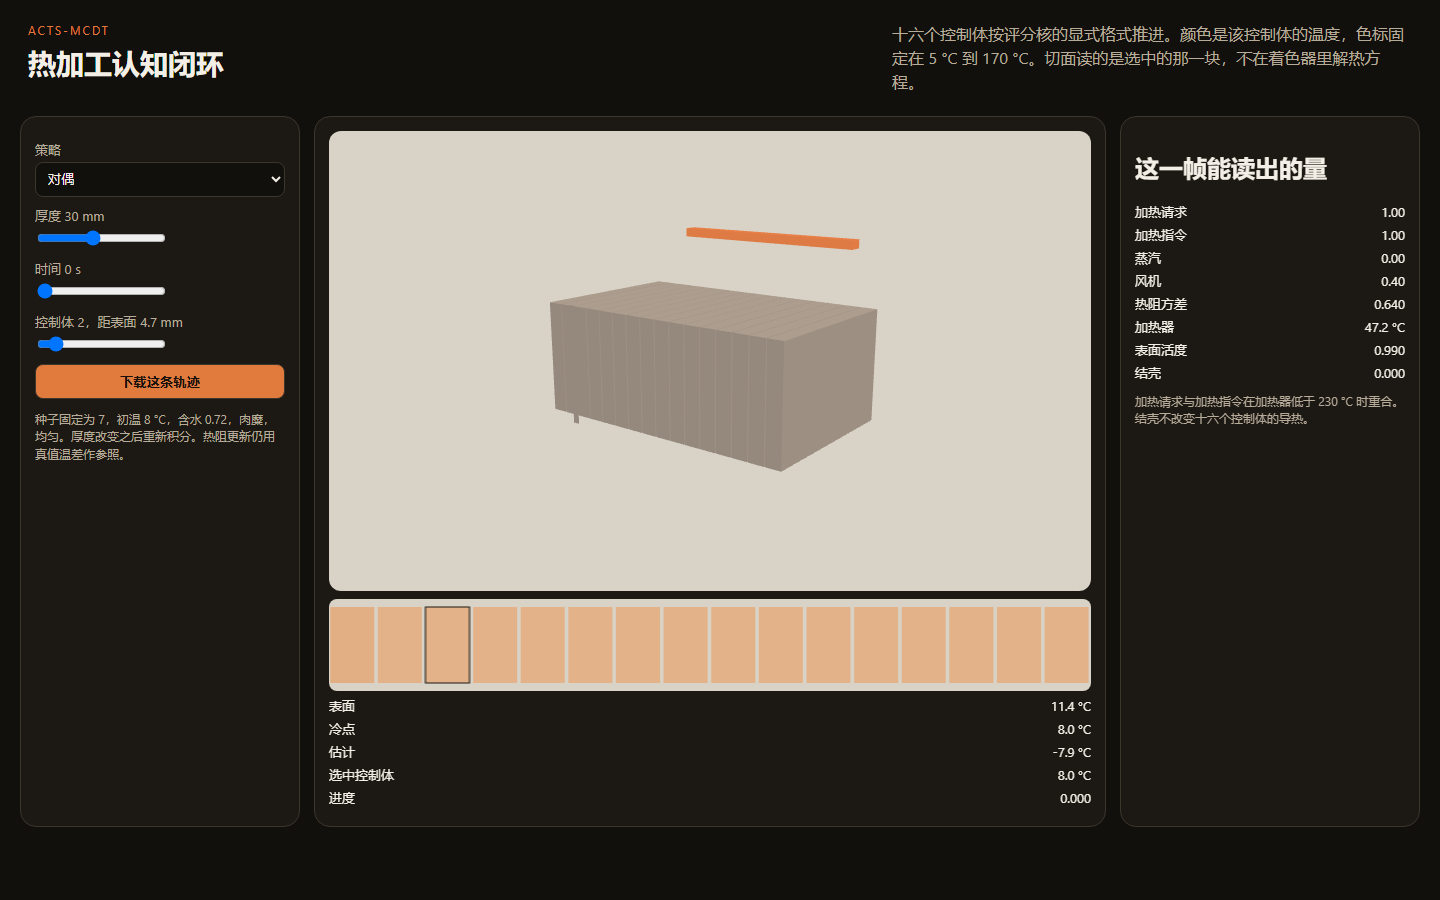
\includegraphics[width=\textwidth]{paper/E_demo_start.png}
\caption{同一条轨迹的起点。表面 $11.4^\circ\mathrm{C}$，冷点 $8.0^\circ\mathrm{C}$，估计 $-7.9^\circ\mathrm{C}$。估计为负，是表面读数减去 16 K 的上限，不是传感器读数。十六块颜色接近，因为场还没有拉开。}
\end{figure}

\begin{figure}[ht]
\centering
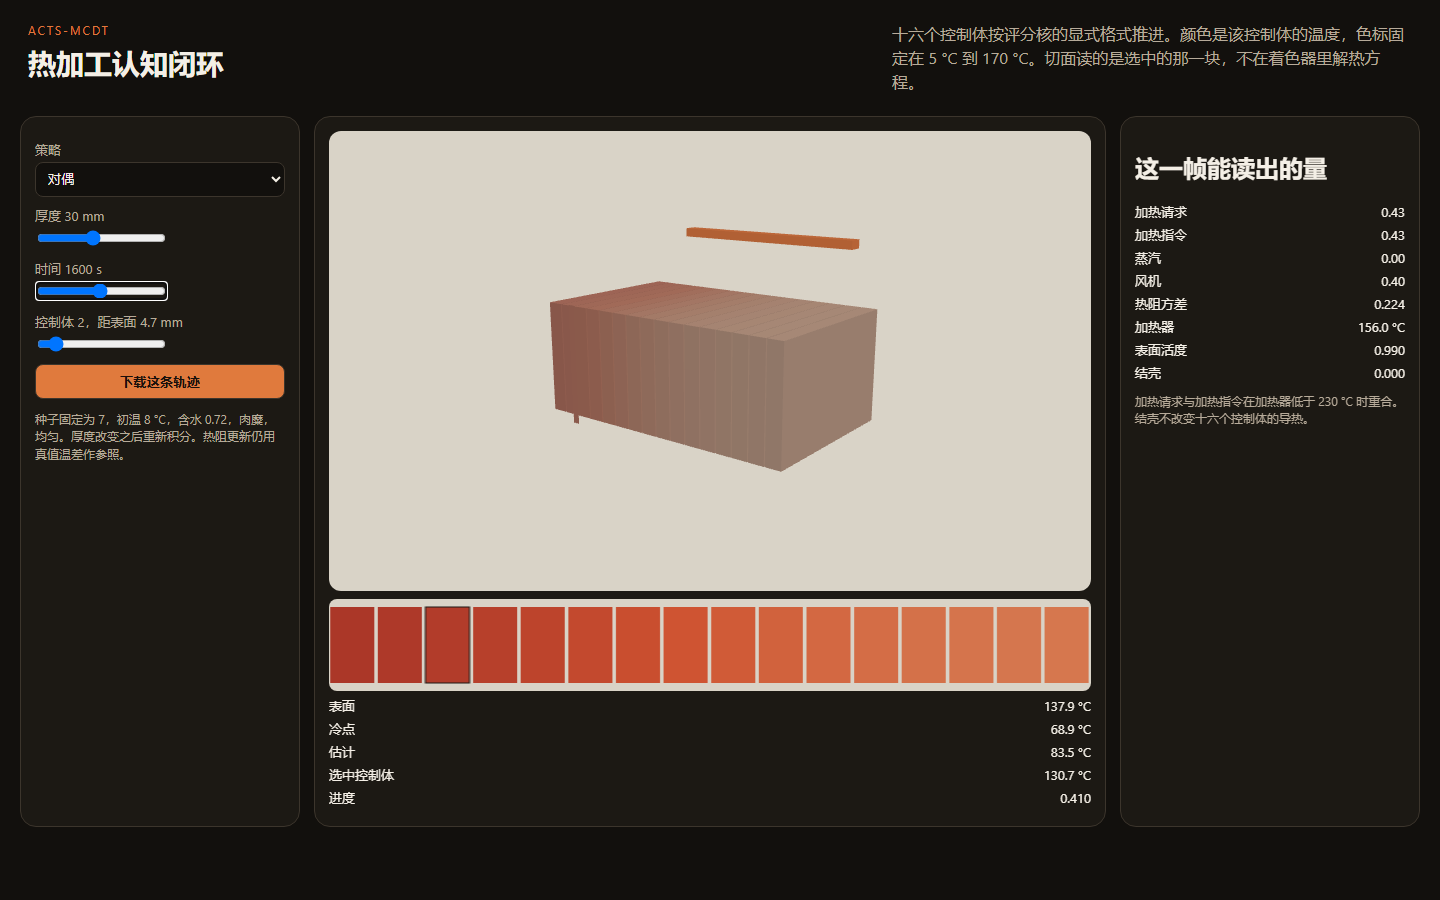
\includegraphics[width=\textwidth]{paper/E_demo_late.png}
\caption{1600 s。表面 $137.9^\circ\mathrm{C}$，冷点 $68.9^\circ\mathrm{C}$，估计 $83.5^\circ\mathrm{C}$，进度 0.410，方差已经是 0.224。色条从表面到深处由深变浅。加热请求与加热指令都是 0.43，加热器 $156^\circ\mathrm{C}$，削减没有动作。}
\end{figure}

加热器是一根细盒子，自发光强度 $0.15+1.3\,u_h$，随投影后的加热变化，不随请求变化。这一项与“强度用投影值”一致。蒸汽、排汽、风速没有标记。没有脂肪层开关。没有探针色带，没有闪动。路径条在侧栏，不在切面旁边，长度来自上一节的显示公式。场景里没有两根针。侧栏文字写过“两节点阶段的切面是表面与冷点的插值”，场景本身没有这句标注，几何上也没有做该插值。

遮挡预置、屏障贴近预置、以及同一种子的一维与二维并置，都还没有放进页面。同一种子的二维轨迹本身也还没有作为预置文件生成。因此当前三维场景不能用来核对遮挡后的探针有效率，也不能用来核对脂肪层是否改变冷点位置。

着色器不积分第二套方程：每一帧只改已有材质的颜色和自发光，再画一次。传热发生在副本的脚本里，而且那是两节点，不是十六条，更不是多孔介质。规格要求三维视图读取数值核的场。当前读的是副本。把副本换成评分核的数组之前，场景上的颜色不能称为主结果的场。

\paragraph{本节不能推出的结论}
画面中有盒子、切面和发热条，不能推出冷点位置、探针时序或屏障动作已经被读出。固定色相窗不是运行内的固定色标。没有轨道和缩放，不能把规格中的相机写成已经提供。未接入的预置不能在演示里当成已经核对的病例。

\chapter{文献分层与继承边界}
\label{ch:lit}

本章要判定的不是文献是否权威，而是模型中的每一层方程从哪里来、哪一层明确不从那里来、以及那一层在本文哪一处被使用。继承表示后文直接使用其方程结构。改写表示边界、状态或判据换成了热加工决策。不继承表示该文献的结论不能被写成本文的结果。条目只讨论可以核到作者、题目和年份的来源。不转写原文句子，不补卷期里没有逐条核对过的页码。

未在本文检索中出现的对象，只记为这次没有读到。未读到不等于不存在。肉类水分等温线在已读入的公开拟合表里条数为零，这是该表的范围，不是对全部肉类测量的否定。

\section{多孔介质与食品热湿传递}

\paragraph{要判定的量}
能量、动量和组分方程在体积平均之后还保留哪些项，以及蒸烤边界上哪些项必须改写。要判定的是冷点能否离开几何中心，不是某一烤箱的升温曲线能否被复现。

\paragraph{继承的文献层与不继承的层}
Whitaker 给出干燥过程中多孔介质里热量、质量和动量同时传递的体积平均理论\cite{whitaker1977}。本文继承平均之后能量、动量与组分方程的结构：固相骨架、液相和气相分别平均，界面交换写成源项，而不是在孔隙尺度上跟踪每一个弯月面。不继承干燥工艺的具体边界，不继承该文为木材或颗粒床选定的对流通量闭合。

Datta 把这一骨架用于食品加工中的同时热质传递\cite{datta2007}。本文继承这个用法：食品被看成含液相与气相的多孔介质，蒸发和冷凝是界面源，而不是把“蒸汽”写成一种更大的导热系数。不继承某一烘箱的实验拟合，也不把该文的某一组物料参数当作本文的主结果。

挤压与油炸多孔介质的系列工作给出蒸发—冷凝源项和压力驱动汽流。本文只把这两类项改写到蒸烤界面：冷凝时潜热进入表面，蒸发时潜热离开表面；压力若升高，只作为气相能否排出的定性约束。不继承油炸外部的热油流动，不继承挤压机的螺杆边界。

Feyissa、Gernaey 与 Adler-Nissen 给出对流烤箱中肉块的三维耦合场，并表明冷点可以偏离几何中心\cite{feyissa2013}。本文继承现象：边界不对称或内部导热不对称时，最低温度不必落在厚度中点。方程改为一维主算例加尚未运行的二维对照。不继承该文的网格、时间步和肉块物料数值。

\paragraph{方程、算法或协议}
体积平均后的能量方程保留四类贡献，写成规格中的结构而不是干燥器的边界条件：
\begin{align*}
\langle\rho c\rangle\partial_t T
&=-\nabla\cdot(q_{\mathrm{cond}}+q_{\mathrm{conv}})\\
&\quad+\dot m_\Gamma\Delta h+q_{\mathrm{rxn}}.
\end{align*}
$q_{\mathrm{cond}}$ 是有效导热，$q_{\mathrm{conv}}$ 是液相或气相携带的显热，$\dot m_\Gamma\Delta h$ 是界面相变，$\ q_{\mathrm{rxn}}$ 是反应热。动量平均只保留到足以说明气相能否在压差下离开表面，不在在线模型里求解完整的孔隙 Navier–Stokes 方程。组分方程保留液相分数与气相分数的交换。

蒸比干热更快进入内部，写成冷凝潜热为正的源，不写成“蒸汽导热更快”。干壳写成近表面渗透率下降，以及有效导热率下降，从而内部热阻上升。评分核没有求解这组平均方程。它用十六条控制体的导热和一条经验潜热通量代替。经验通量 $18000\,u_{\mathrm{st}}(1-a_w)$ 的量级是瓦每平方米，不是 $\Delta h$ 乘以由分压算出的质量流。模块里写着的 $2.3\times 10^{6}\,\mathrm{J/kg}$ 没有乘进战役步进。因此日志里的温度不是 Whitaker 方程的解。

冷点偏离几何中心在评分核里只有两个来源。\texttt{hetero}=1 把初始温度铺成 $\pm 4^\circ\mathrm{C}$ 的空间倾斜，最低温可以不在中心，但这是初始条件，不是边界驱动的偏移。\texttt{hetero}=2 把下标为 $5$ 的控制体导热降到 $0.45$ 倍，热阻位置固定在大约三分之一厚度处。这是一维夹层，不是\cite{feyissa2013}的三维几何。二维截面尚未运行，不能把该现象写成已经复现。

\subsection{来源对照}
\begin{table}[ht]
\centering
\caption{传递骨架。方式一列只说明本文用到哪一层。}
\begin{tabularx}{\textwidth}{lXll}
\toprule
来源 & 使用的结果 & 方式 & 不继承 \\
\midrule
Whitaker, 1977 & 体积平均后的能量、动量与组分 & 结构 & 干燥工艺的边界 \\
Datta, 2007 & 食品中同时热质传递 & 用法 & 某一烘箱的拟合 \\
挤压与油炸系列 & 蒸发—冷凝源、压力驱动汽流 & 改到蒸烤界面 & 油炸外部流动 \\
Feyissa 等, 2013 & 冷点可偏离几何中心 & 现象 & 该文网格与物料数 \\
\bottomrule
\end{tabularx}
\end{table}
挤压与油炸系列在这次检索里没有单独的文献条目，表中只保留现象层的改写，不补未核对的卷期。

\paragraph{本节不能推出的结论}
引用体积平均理论不能推出本文已经求解多孔介质真值。一维夹层的冷点移动不能代替三维烤箱里的冷点云图。油炸文献中的外部流动不能写成蒸烤腔的风场。

\section{水分活度、收缩与各向异性}

\paragraph{要判定的量}
含水率 $M$ 与水分活度 $a_w$ 是否被写成同一个量，以及导热、厚度、渗透率里哪些参数有文献区间、哪些只能做灵敏度。要判定的还包括：已读入的等温线能约束哪一类物料、约束到哪一个温度。

\paragraph{继承的文献层与不继承的层}
食品水分等温线的综述传统给出 $a_w$ 与含水率的非线性关系。GAB 形式
\[
M=\frac{M_0 C K a_w}{(1-K a_w)\,(1-K a_w+C K a_w)}
\]
作为该关系的一种闭合被继承\cite{gab1980,sorption2026}。Timmermann 对多层吸附参数的比较说明，BET 与 GAB 的参数相关，数值上可以病态\cite{gab1980}。本文继承这一警告：三个参数不单独解释，相关结构必须保留。不继承未经测定的 $M_0,C,K$ 数值，也不把拟合表里的数写成新的实验测定。

Clausius–Clapeyron 关系使吸附热随温度移动等温线。本文继承“温度升高时单层容量下降”这一方向。不继承把活度当成含水率本身，也不继承测定温度以外的外推数值。

Choi 与 Okos 给出组分热物性随温度和组成变化的加和传统\cite{choi1986}。本文继承 $k$ 随水分、脂肪和温度变化的趋势。不继承把各向同性标量当成全部导热信息。各向异性测量给出 $k_\parallel\neq k_\perp$。本文把它写成张量结构。不把某一品种的单点测量当成普遍常数。

蛋白受热收缩与孔隙变化的工艺文献给出厚度和渗透率随蛋白进度变化。本文写成收缩方程。不把收缩定义成品。收缩是几何与阻力的演化，品质进度仍由动力学积分定义。

\paragraph{方程、算法或协议}
活度进入表面蒸发的驱动力是 $a_w p_{\mathrm{sat}}(T_s)-p_v$，不是 $M$ 本身。因此同一含水率在淀粉与蛋白上可以对应不同的界面蒸汽压。评分核没有反演 GAB 代数。它用单调代理
\[
a_w=1-\mathrm{e}^{-m/s}(1-0.15\,k),
\]
土豆、面团、肉糜的尺度 $s$ 分别取 $0.055$、$0.08$、$0.10$，$k$ 取 $0.80$、$0.75$、$0.70$，再裁剪到 $[0.02,0.99]$。土豆的尺度靠近已读表里 $60^\circ\mathrm{C}$ 附近的单层容量量级，但代理不是该表的拟合残差。肉糜的尺度是宽而弱的信息，因为该表中肉类曲线条数为 $0$。未读到不等于不存在：本文没有读到可引用的肉类等温线文件，所以肉类活度保持为开放参数，不用淀粉的 $M_0,C,K$ 冒充。

温度移动只在测定范围内解释。公开表中土豆的清洁曲线到 $60^\circ\mathrm{C}$ 为止。烤制表面高于此温度时，GAB 数值是外推，不能进入主结果。$M_0,C,K$、$k_\parallel/k_\perp$ 和收缩系数在没有文献区间时只进入灵敏度扫描。

各向异性写成
\[
\vect{k}_{\mathrm{eff}}=k_\perp(M,S)\,\vect{I}+(k_\parallel-k_\perp)\,\vect{e}\otimes\vect{e}.
\]
脂肪夹层的热阻是 $L_{\mathrm{fat}}/(k_{\mathrm{fat}}A)$，加在冷点路径上。评分核没有这个张量。均匀导热率是 $0.68\,\mathrm{W/(m\cdot K)}$，只有下标 $5$ 的控制体在 \texttt{hetero}=2 时降到 $0.45$ 倍，即 $0.306\,\mathrm{W/(m\cdot K)}$。这是标量缺损，不是各向异性。

\subsection{来源对照}
\begin{table}[ht]
\centering
\caption{界面与结构闭合。没有单独条目的综述只记传统，不补页码。}
\begin{tabularx}{\textwidth}{lXll}
\toprule
来源 & 使用的结果 & 方式 & 不继承 \\
\midrule
GAB 形式 \cite{gab1980,sorption2026} & \(a_w\) 与含水的非线性 & 形式 & 未测定的 \(M_0,C,K\) \\
Clausius--Clapeyron 传统 & 等温线随温度移动 & 方向 & 把活度当成含水 \\
组分加和 \cite{choi1986} & \(k\) 随水分和脂肪变化 & 趋势 & 各向同性即全部 \\
各向异性测量传统 & \(k_\parallel\neq k_\perp\) & 张量结构 & 单点当普遍常数 \\
收缩工艺传统 & \(L\) 与渗透率随进度变化 & 演化方程 & 收缩即品质 \\
\bottomrule
\end{tabularx}
\end{table}

收缩规格是
\[
\dot L=-\beta_s L_0\dot\alpha_p,\qquad K=K_0(L/L_0)^{n_K}\varepsilon_g^{n_\varepsilon}.
\]
评分核的厚度在一次运行内不变。结壳变量 $S$ 只进入热阻代理 $r_{\mathrm{proxy}}=\mathrm{clip}(\Delta T/8+1.2+2.5 S,\,0.8,\,8)$，不改变网格间距。渗透率不在状态里。因此日志不能检验收缩与内部蒸汽排出的耦合。

\paragraph{本节不能推出的结论}
清洁拟合的分位数不能描述全部食品，也不能验证冷点、探针或烤制。代理活度下降不能写成 GAB 三参数已被辨识。一维导热缺损不能写成各向异性测量。

\section{反应进度与热力当量}

\paragraph{要判定的量}
品质是一条温度阈值，还是一条速率方程的积分。要分开的是冷点上的热力进度、表面褐变和含水开关。颜色能不能代替中心进度，是本节必须否定的用法。

\paragraph{继承的文献层与不继承的层}
van Boekel 说明食品品质动力学用速率方程，Arrhenius 只是其中一种温度依赖\cite{vanboekel2008}。本文继承速率方程这一层，温度依赖在规格中仍用 Arrhenius，并保留其适用范围：温度窗口、水分开关和反应物是否耗尽都要写明。不把所有品质都写成一级反应。

Holdsworth 关于热力杀菌的标准表述把 $F$ 值沿冷点历史积分\cite{holdsworth1997}。本文把它写成进度 $\alpha_m$，不把 $\alpha_{\mathrm{safe}}$ 写成法规限值。$\alpha_{\mathrm{safe}}$ 与分位、滞回一样是设计量。

蛋白变性、淀粉糊化和美拉德的动力学实验表明三类进度对水分的开关不同。本文写成 $g_i(\varepsilon_l,S)$。不继承用颜色代替中心进度。美拉德文献只解释表面色泽，也就是路径 B 所接触的那一类表面反应。它不提供冷点是否达到热力进度的证据。微生物文献只提供积分形式。初始污染量不在状态向量中，绝对菌数也不进入决策。

\paragraph{方程、算法或协议}
规格中的速率是
\[
\dot\alpha_i=A_i\exp\big(-E_{a,i}/RT\big)\,g_i(\varepsilon_l,S)\,\alpha_i^{n_i},
\]
其中 $n_i$ 不必为 $1$。热力当量沿冷点写成
\[
F=\int_0^t 10^{(T_{\mathrm{cold}}(s)-T_{\mathrm{ref}})/z}\,\mathrm{d}s,
\]
再映射到 $\alpha_m$。评分核没有使用 Arrhenius 形式，也没有分别积分蛋白、淀粉和美拉德。它只在冷点上累积
\[
\dot f=10^{(T_{\mathrm{core}}-70)/10}/60,\qquad\alpha_m=1-\mathrm{e}^{-f/2}.
\]
参照温度 $70^\circ\mathrm{C}$，$z=10\,\mathrm{K}$，时间以秒计再除以 $60$，所以 $f$ 的单位是分钟量级的等效时间。映射 $\alpha_m=1-\mathrm{e}^{-f/2}$ 把等效时间压进 $(0,1)$。当 $f\to\infty$ 时 $\alpha_m\to 1$，于是 $e_\alpha=\alpha_m-0.85$ 的上沿是 $+0.15$。这个上沿是饱和，不是测量精度。

表面褐变在评分核里是另一条经验式：表面温度超过 $110^\circ\mathrm{C}$ 且表面含水低于 $0.55$ 时才增加。它不进入 $\alpha_m$。因此同一条温度史上，中心进度和表面色泽可以分开。这与“颜色不代替中心进度”一致，但系数 $2\times 10^{-4}$ 没有文献区间，只能留在实现里，不能进入主结果的参数表。

设计线 $0.85$ 只用于定义 $e_\alpha$。停机时 $\alpha_m<0.85$ 记为负误差，表示停在设计线之下。它不是认证通过线。腔温闭环的中位 $e_\alpha$ 为 $+0.15$，对应进度已经饱和，不能读成“比设计线精确高出 $0.15$”。

\subsection{来源对照}
\begin{table}[ht]
\centering
\caption{进度，而不是温度阈值。}
\begin{tabularx}{\textwidth}{lXll}
\toprule
来源 & 使用的结果 & 方式 & 不继承 \\
\midrule
van Boekel, 2008 & 品质用速率方程 & 速率层 & 全部写成一级反应 \\
Holdsworth, 1997 & \(F\) 沿冷点历史积分 & \(\alpha_m\) 的形式 & 法规限值 \\
蛋白、淀粉、美拉德传统 & 水分开关不同 & \(g_i(\varepsilon_l,S)\) & 颜色代替中心进度 \\
\bottomrule
\end{tabularx}
\end{table}
后一行没有单独条目。评分核也没有分开这三类积分。

\paragraph{本节不能推出的结论}
$F$ 的积分形式不能推出初始菌数，也不能推出法规限值已经被满足。美拉德路径上的表面色泽不能推出冷点安全。评分核的 $z$ 值映射不能当成 Arrhenius 参数已经拟合。

\section{逆热传导与可观测性}

\paragraph{要判定的量}
表面温度的采样加密以后，内部热阻的信息是否增加。要判定的是线性化秩，以及集合更新里哪些量可以当决策量。稳态、无相变、无内部梯度时，答案应为零灵敏度。

\paragraph{继承的文献层与不继承的层}
Özisik 与 Orlande 给出逆热传导对高频噪声指数放大的结构\cite{ozisik2000}。本文继承病态性：把表面温度历史反推内部热流或内部热阻时，高频成分被放大，正则化是估计问题的一部分。不把他们的某一正则化算法当成唯一估计器。

Beck 的序贯估计传统用未来时间步稳定热流估计。本文只把它当作病态程度的参照：需要向未来看多远，说明当前观测有多弱。不作为在线主算法，也不把整机问题降成单层壁面。

线性系统的可观测性与 Kalman 更新提供秩条件和协方差更新。本文只在两节点命题里使用这一层。不继承“线性模型覆盖相变”。在 \eqref{eq:twonode} 里潜热与腔温的输入列共线；离开平衡之后，气流段仍可以使 \(R_{\mathrm{ext}}\) 与 \(R_{\mathrm{int}}\) 的灵敏度列分开。线性化只在相变方向已经给定的短区间内使用。

Evensen 给出集合卡尔曼滤波的预测—分析格式\cite{evensen2003}。本文把它定为场层估计的规格：集合先按模型推进，再用观测做分析更新。不把集合均值当成决策量。停止看的是进度的下分位。集合均值“看起来已经熟了”不能通过。

\paragraph{方程、算法或协议}
两节点线性化后，仅腔温扰动时输入矩阵是单列。潜热也只进入表面节点，输入列与腔温列共线，变号不增加秩。紧接着只改外部热阻的气流段，使 $(R_{\mathrm{ext}},R_{\mathrm{int}})$ 的灵敏度列不能互为标量倍。这是本文在蒸烤边界上的推论，不是\cite{ozisik2000}或\cite{evensen2003}的原定理。证明自洽地比较两段特解：冷凝项进入表面节点时不经过外部热阻；气流段只改外部热阻。输入列共线并不取消这个参数列的结论。

数值核对用的不是逆问题算法。两段脉冲的表面—内部滞后为 $40.846$，单独蒸汽为 $38.912$，判据是差值大于 $1$。没有声称这是 $1.15$ 倍。稳态极差为 $0$，表示平衡温度里读不出三组热阻的差别。

评分核的在线估计不是集合卡尔曼滤波。它是标量滞后
\[
\widehat T_c\leftarrow\widehat T_c+\Delta t\,(y_T-\widehat T_c)/\tau,
\]
再把估计压到表面观测之下，并用探针窗口更新一个标量 $\hat r$ 及其方差。方差的先验是 $0.64$。更新被接受时乘 $0.35$，即降到 $0.224$。这不是 $\log\det$ 的信息增益，也没有集合。集合规模 $32$ 与 $128$ 没有进入主日志。在线 Fisher 矩阵没有运行。

噪声幅度 $0.4^\circ\mathrm{C}$ 是确定性散列，不是\cite{ozisik2000}里用来展示指数放大的随机高频序列。用该幅度不能回推逆问题的放大倍数。

\subsection{来源对照}
\begin{table}[ht]
\centering
\caption{表面温度为什么不够。序贯估计传统没有单独条目。}
\begin{tabularx}{\textwidth}{lXll}
\toprule
来源 & 使用的结果 & 方式 & 不继承 \\
\midrule
Özisik、Orlande, 2000 & 高频噪声被放大 & 病态结构 & 唯一正则化算法 \\
序贯估计传统 & 未来步稳定热流估计 & 病态参照 & 整机降成单层壁 \\
可观测性与 Kalman 更新 & 秩与协方差 & 两节点命题 & 线性模型覆盖相变 \\
Evensen, 2003 & 预测—分析格式 & 场层规格 & 集合均值当决策量 \\
\bottomrule
\end{tabularx}
\end{table}

\paragraph{本节不能推出的结论}
稳态极差为 $0$ 只支持“平衡观测不含内部热阻”，不支持内部状态已经被重构。标量方差下降不支持集合卡尔曼滤波已经运行。病态性文献不提供本文的正则化参数。

\section{信息价值与对偶控制}

\paragraph{要判定的量}
一次阀门动作是在推动品质，还是在做一次实验。要判定的是信息有没有下降；没有下降时，停止时刻是否保持不动。家电执行器不能发出任意波形，因此还要判定探针库是不是该问题的可执行子集。

\paragraph{继承的文献层与不继承的层}
Lindley 把实验提供的信息定义为先验熵与后验熵之差\cite{lindley1956}。本文的 $G(a)$ 采用这一层。不把效用只写成参数熵。决策熵看的是 $\vect{z}$ 里与停止、表面品质和均匀性有关的分量，不是全部物性参数的熵。

Fedorov、Kiefer 等最优实验设计给出 $\log\det$ 与参数置信椭球。本文只把 Fisher 形式当作对照。不把离线一次性设计代替在线脉冲。二者排序不一致时以集合形式为准；而集合形式本身尚未作为主结果跑完，所以 Fisher 对照也还没有排序可报。

Feldbaum 的对偶控制说明控制量同时影响状态与信息\cite{feldbaum1965}。本文继承问题提法：输入既出现在状态方程里，也出现在信息增益里。不继承其原问题的解析解。家电的加热、蒸汽、风速和排汽不是任意波形。

谨慎控制与主动学习控制把有限时域上的信息与代价并列。探针库是该问题的可实现子集。不把家电执行器当成任意波形发生器。

\paragraph{方程、算法或协议}
信息增益的规格是
\[
G(a)=\frac12\log\det\Sigma_z(t)-\frac12\log\det\Sigma_z(t+\tau;a).
\]
代价是能量、失水、表面褐变和时间的加权。探针只在 $G$ 超过下限且损伤低于预算时执行。P4 的顺序由秩条件固定：先相变变号，再对流切换。无效则停止时刻不动。评分核没有计算 $G(a)$。它用固定窗口 $[150,190)\,\mathrm{s}$ 代替在线打分，用“是否更接近 $r_{\mathrm{proxy}}$”代替熵差，用方差乘 $0.35$ 代替 $\log\det$ 的下降比例。窗口不随赤字开关。赤字大于零但方差已经不大于 $0.25$ 时，核不再进入探针。这是一条阈值规则，不是在探针库上最大化信息增益减去代价。

厚件上还有一条与信息有关、但不是熵的否决：对偶且方差仍大于 $0.45$、厚度大于 $0.04\,\mathrm{m}$ 时，即使冷点估计已经越过裕量，也不停止。这是否决，不是 $G(a)$ 的数值。

厚度上的定性只能引用第 10 章已经汇总的交叉：薄件上探针没有把对偶从无探针优化里分开，两者都停在设计线之下；中等厚度上对偶把中位误差从约 $-0.53$ 拉到约 $-0.08$；厚件上两者都提前，对偶只略好。精确交叉格以第 10 章的表为准。这些差别是停止误差，不是 $G(a)$ 的测量。

\subsection{来源对照}
\begin{table}[ht]
\centering
\caption{动作为什么可以是一次实验。最优设计与谨慎控制没有单独条目。}
\begin{tabularx}{\textwidth}{lXll}
\toprule
来源 & 使用的结果 & 方式 & 不继承 \\
\midrule
Lindley, 1956 & 信息是熵差 & \(G(a)\) 的层 & 效用只写参数熵 \\
最优设计传统 & \(\log\det\) 与置信椭球 & Fisher 对照 & 离线设计代替脉冲 \\
Feldbaum, 1965 & 输入同时推动状态与信息 & 问题提法 & 原问题的解析解 \\
谨慎控制传统 & 有限时域并列信息与代价 & 探针库 & 任意波形 \\
\bottomrule
\end{tabularx}
\end{table}

\paragraph{本节不能推出的结论}
对偶问题的提法不能推出解析最优波形已经得到。固定窗口不能写成在线信息最大化。方差乘 $0.35$ 不能写成 Lindley 熵差。中等厚度上的误差变化不能单独证明探针库优于连续对偶控制。

\section{算子学习}

\paragraph{要判定的量}
神经算子是加速器还是定律。要判定的是同一训练集上，哪一个候选在蒸汽干预的位移误差上更低。文献不提供这个胜负。

\paragraph{继承的文献层与不继承的层}
Raissi、Perdikaris 与 Karniadakis 给出用残差惩罚方程的训练方式\cite{raissi2019}。本文只把它当作训练时的物理损失项。不用该网络代替在线安全判断。安全投影的自变量不含网络输出。

Li 等给出用 Fourier 神经算子学习参数化演化的结构\cite{li2021fno}。本文把它列为候选 $\mathcal{G}_\phi$。不继承训练分布之外的精度保证。

Lu 等给出 DeepONet 的分支—主干结构\cite{lu2021deeponet}。本文把它列为同一数据上的对照算子。不继承“一种结构优于另一种”的普遍结论。

\paragraph{方程、算法或协议}
候选算子学习的是边界到决策状态的映射，而不是一个新的本构关系。选择规则是：同一训练集上，蒸汽干预造成的位移误差更低者为主模型。另一个保留为对照。残差超过预设上界时回退到物理步进，不把算子输出送进屏障。

这次没有训练，没有干预位移误差的表，没有残差界的回退次数。Fourier 算子和 DeepONet 都停留在规格。评分核的十六条步进是唯一跑过的演化。它的截断误差来自空间步长 $L/16$ 和固定步长 $2\,\mathrm{s}$，不是来自神经算子的泛化误差。

主模型尚未选出，因此任何“算子已经加速了试验”的句子都没有对象。教师扩充标记也没有进入主表。

\subsection{来源对照}
\begin{table}[ht]
\centering
\caption{加速器，不是定律。}
\begin{tabularx}{\textwidth}{lXll}
\toprule
来源 & 使用的结果 & 方式 & 不继承 \\
\midrule
Raissi 等, 2019 & 残差惩罚方程 & 训练损失项 & 网络代替安全判断 \\
Li 等, 2021 & Fourier 算子 & 候选 \(\mathcal{G}_\phi\) & 训练外的精度保证 \\
Lu 等, 2021 & 分支—主干 & 同一数据上的对照 & 一种结构普遍更优 \\
\bottomrule
\end{tabularx}
\end{table}

\paragraph{本节不能推出的结论}
两篇算子文献不能推出谁在蒸烤干预上更准。物理损失项不能推出在线安全已经由网络保证。未运行的回退次数不能画成曲线。

\section{因果、预测控制与安全过滤}

\paragraph{要判定的量}
蒸汽干预的效应能否按路径相加，以及安全可行域是否随后验变形。要判定的还有：硬回路的存在是算法结论，还是器具安全框架提出的要求。

\paragraph{继承的文献层与不继承的层}
Pearl 区分预测、干预和反事实，并把 $\mathrm{do}$ 定义成替换结构方程\cite{pearl2009}。本文按这个顺序计算路径 A、B、C：先预测，再替换蒸汽节点，最后才在需要时做反事实对比。不从短烹饪序列里发现父节点。父节点是规格里写死的，不由数据搜索改写。

Rawlings、Mayne 与 Diehl 给出有限时域约束优化这一类问题\cite{rawlings2017}。本文的预测控制属于这一类。不继承某一求解器的默认最优性声明。

Ames、Xu、Grizzle 与 Tabuada 给出屏障函数约束下的二次投影\cite{ames2017cbf}。本文继承投影形式：在安全约束下，把动作改到离参考动作最近的可行点。不继承“屏障条件自动等于器具安全认证”。

IEC 60335-1 与 GB 4706.1 给出家用电器在漏电、温升和异常工作上的安全框架\cite{iec60335,gb4706}。本文只继承“硬回路必须存在，且不读取品质后验”这一要求来源。不把标准条款写成算法已经满足。实施时用的是现行条款的入口，不是本文重新编号的合格声明。

\paragraph{方程、算法或协议}
路径可加是链式法则。少掉 C，结壳后期没有项。短探针窗口内 C 是小量，全时域积分必须保留。干预计算把蒸汽节点替换为接管值；条件相关则保留策略到蒸汽的边。二者不是同一个数。

预测控制的规格是有限时域上最小化品质代价，约束写成机会约束，探针占用区间内输入等于已经发布的探针。求解器被指定为 CasADi/IPOPT。这次没有调用该求解器。评分核里名为无探针优化和对偶的两支，用的是估计温度的饱和线性请求，不是有限时域优化的解。因此日志不能支持“求解器已声明最优”。

投影的规格是
\[
\vect{u}=\argmin_{\vect{u}}\|\vect{u}-\vect{u}_{\mathrm{AI}}\|_W^2
\]
并满足 $\dot h_j+\gamma_j h_j\ge 0$。$h_j$ 的自变量只有漏电、水位或干烧、加热器温度、腔压和门。后验只通过参考点进入目标。命题是：可行域与后验不交。断言实现的是一条测试函数，不是二次规划：加热器超过 $210^\circ\mathrm{C}$ 时把请求剪到 $0.25$，两个不同后验得到同一个剪裁；加热器低于该阈值时保持 $1$。物理核的削减从 $230^\circ\mathrm{C}$ 开始，按 $(T_h-230)/40$ 最多削减 $75\%$，作用在已经形成的请求上。$210$ 与 $230$ 是两个对象。测试函数通过，只说明“不随后验改变”这一方向；它不说明二次规划已经求解，也不说明标准条款已经满足。

硬件切断不读估计器。这一句是结构要求。本次日志没有漏电、水位、腔压和门的采样，不能用加热器削减代替整条硬回路。

\subsection{来源对照}
\begin{table}[ht]
\centering
\caption{解释与执行。}
\begin{tabularx}{\textwidth}{lXll}
\toprule
来源 & 使用的结果 & 方式 & 不继承 \\
\midrule
Pearl, 2009 & \(\mathrm{do}\) 是替换结构方程 & 路径顺序 & 从短序列发现父节点 \\
Rawlings 等, 2017 & 有限时域约束优化 & 问题类 & 求解器默认最优 \\
Ames 等, 2017 & 约束下的二次投影 & 投影形式 & 自动等于器具认证 \\
IEC 60335-1，GB 4706.1 & 漏电、温升、异常工作 & 硬回路必须存在 & 条款写成算法已满足 \\
\bottomrule
\end{tabularx}
\end{table}

\paragraph{本节不能推出的结论}
路径公式不能从短序列里发现新的父节点。饱和线性请求不能写成模型预测控制的最优解。屏障测试函数通过不能写成器具已经按安全标准认证。标准文本不提供软件投影的数值参数。

\section{创新所在的层}

\paragraph{要判定的量}
新的对象是一条方程，还是几条已经存在的方程之间的连接。本节把前面各节的“不继承”列收束成四条连接，并规定怎样退出创新表述。

\paragraph{继承的文献层与不继承的层}
多孔介质方程、熵差、$\mathrm{do}$ 算子、神经算子和屏障函数都已经有来源\cite{whitaker1977,lindley1956,pearl2009,li2021fno,lu2021deeponet,ames2017cbf}。这些层全部不作为本文新创造的对象。不继承“把连接说成新的本构、新的熵或新的屏障定义”。

\paragraph{方程、算法或协议}
新增的是四条连接。

\begin{enumerate}
\item 决策状态 $\vect{z}$ 从全场中取出，并与稳态不可辨识接在一起：平衡且无相变时，内部热阻不进入代数方程，灵敏度列消失。稳态腔温再密也不更新 $R_{\mathrm{int}}$。信息动作必须离开平衡。
\item 信息动作落成 P4：相变变号之后接对流切换。方差或分位没有下降时，停止时刻保持在动作之前。这是无效探针否决，不是新的熵定义。
\item 同一次蒸汽干预分解为三条路径：潜热到冷点，表面水分到品质，结壳到内部热阻再到冷点。少一条，结壳后期的热阻没有解释项。
\item 品质后验与安全可行域使用不相交的测量。品质链可以错，可行域的形状不随后验改变。硬件切断不读估计器。
\end{enumerate}

这四条若与某篇已发表论文的技术方案相同，改为引用并退出创新表述。本文没有把“未读到”写成“不存在”。肉类等温线、公开的烤制中心温度历程、以及与这四条连接完全相同的技术方案，都只在已经读到的范围内讨论。

评分核实现了这四条里的一部分，而且是简化以后的部分。决策状态在日志里只保留冷点、表面、进度、热阻代理和方差，没有表面褐变进入停止规则，没有温度离散的决策项。P4 被固定时间窗代替，否决只在厚件且方差仍高时出现。三条路径没有在评分核里按链式法则计算，浏览器里的三条显示公式更不能算实现。测量隔离只落实到加热器温度这一路硬测量；漏电、水位、腔压和门没有进入这次步进。因此四条连接是本文的结构主张，不是这次日志已经逐项跑完的清单。

\paragraph{本节不能推出的结论}
四条连接不能改写 Fourier 定律，不能替换熵的定义，也不能替换屏障函数的定义。部分实现不能写成四条都已在主结果里定量成立。未检索到相同技术方案，只说明本次阅读没有遇到，不说明文献中没有。

\chapter{图件总表}
\label{ch:figures}

本章按图位登记对象、坐标、来源和不能支持的句子。图位分为机制图、数学图、数据图和实施例图。基础部分为机制图 28 幅、数学图 16 幅、数据图 24 幅、实施例 8 幅。扩展面板 D25--D36 仍从同一日志取列，不新增科学主张。合计 88 个图号。分面板用 (a)(b)(c)，不另计图号。

已经画出的数据图是 D1、D6、D7、D10、D25，图放在第 \ref{ch:sim} 章，这里不再重复插入。其余数据图位没有对应日志，不绘制曲线。Q1--Q6 的证明几何放在第 \ref{ch:proof} 章。本章不把证明几何再画一遍，只登记每个图位能支持哪一句、不能支持哪一句。
\section{机制图}

机制图表达变量之间的依存。图中的箭来自已经写出的方程或模块合同。没有测量的边不标数值。

\subsection{M1 四个决策与信息赤字}
\paragraph{对象}
四个判断——能否停止、表面含水是否偏离、温度是否仍在散开、继续施加边界是否安全——各自对信息赤字 $\Delta\mathcal{I}$ 的贡献。

\paragraph{坐标与应读出的关系}
横轴是四个判断，纵轴是该判断的剩余熵减掉允许误判。柱高于零表示这个判断仍缺信息。四个柱可以同时为正，也可以只有停机为正。

\paragraph{与方程的对应}
赤字的定义在第 1 章：$\Delta\mathcal{I}=H(\phi(\vect{x})\mid\vect{y}_{0:t})-H_{\mathrm{tol}}$。$\phi$ 分别取冷点进度、表面含水、温度标准差和硬安全指示。四条柱不共享一个阈值。

\paragraph{来源}
机制图。它不读取 S1 日志。允许误判由动作切换的滞回带决定，本次没有用外部温度历程标定 $H_{\mathrm{tol}}$。

\paragraph{该图位允许支持的句子}
可以写：停机赤字与表面赤字是两个泛函，腔温采样只进入边界输入，不自动降低内部进度的熵。

\paragraph{该图位不能支持的句子}
不能把柱高写成某一菜谱还要几分钟。不能把四个判断合并成一个“熟度百分比”。

\subsection{M2 六步闭环与真值隔离}
\paragraph{对象}
真值生成、带噪采样、后验、安全投影、写回边界、用真值场评分，这六步的数据流，以及真值不得进入在线模块的切口。

\paragraph{坐标与应读出的关系}
六步沿环排列。切口画在第 2 步：在线模块的输入只有可安装通道。评分箭从真值场指向指标，不指向执行器。

\paragraph{与方程的对应}
完整性条件是第 1 章的六条。热阻更新若使用由真值温差构成的 $r_{\mathrm{proxy}}$，箭头就穿过了切口。

\paragraph{来源}
机制图，对照本次核的接口。核在“是否更接近参照”这一步读了真值温差，所以图上该箭要标成已发生的泄漏，而不是理想环。

\paragraph{该图位允许支持的句子}
可以写：本次方差下降必须和参照一起报告，因为参照不是传感器。

\paragraph{该图位不能支持的句子}
不能把画成闭环的箭头写成异构真值已经隔离。积分器是十六条控制体，不是带压力方程的多孔介质真值。

\subsection{M3 五层与唯一执行器接口}
\paragraph{对象}
物理场、决策状态、估计、解释、执行五层，以及只有执行层能写执行器。

\paragraph{坐标与应读出的关系}
五层自上而下。向下的箭只携带分布或分位数。唯一向上写回执行器的箭从安全投影出发。

\paragraph{与方程的对应}
模块合同在第 3 章：层间不传递对方的内部数组。品质模型的输出在进入执行器前被只依赖硬测量的不等式投影。

\paragraph{来源}
机制图。本次实现把积分、策略和评分放在同一次循环里，层间隔离没有落在目录边界上。

\paragraph{该图位允许支持的句子}
可以写：合同要求控制器读分位数；本次跟踪器交出的是 $(\hat T_c,\hat r,\mathrm{Var}(r))$ 三个标量。

\paragraph{该图位不能支持的句子}
不能把五层框图写成五个进程已经分开部署。

\subsection{M4 四个时间尺度的中断}
\paragraph{对象}
电气安全、热安全、信息探针、品质菜单四个时间尺度，以及快环打断慢环的方向。

\paragraph{坐标与应读出的关系}
横轴是时间尺度的量级：毫秒至秒、秒、数十秒、分钟。箭头只能从更快的环指向更慢的环，表示打断。

\paragraph{与方程的对应}
探针窗 40 s 位于信息尺度。品质菜单是 $900$、$1170$、$1530$ s。加热器时间常数约 $43$ s，与探针窗同一量级，所以探针期间加热器状态不能当成已达平衡。

\paragraph{来源}
机制图，常数来自附录的尺度算术，不是示波器记录。

\paragraph{该图位允许支持的句子}
可以写：停机后的低功率仍可能继续累积 $F$，评价必须用停机时刻的 $\alpha_m$。

\paragraph{该图位不能支持的句子}
不能把四个尺度写成已经由中断优先级的代码实现。本次模式整数只有品质、探针和保持。

\subsection{M5 模块合同只传递分布}
\paragraph{对象}
估计模块交给控制模块的对象是 $p(\vect{z}\mid\vect{y})$，不是一个点估计。

\paragraph{坐标与应读出的关系}
左侧是观测，中间是后验，右侧是机会约束使用的分位。点估计若出现，只能作为对照箭，并且标成合同之外。

\paragraph{与方程的对应}
决策充分性要求代价是 $\vect{z}$ 的 Lipschitz 函数，并且后验不确定度低于切换滞回。均值一个数不包含不确定度，因此不满足合同。

\paragraph{来源}
机制图。本次加热律用的是 $\hat T_c$ 加一条由 $\sqrt{\mathrm{Var}}$ 写成的裕量，裕量不是后验分位。

\paragraph{该图位允许支持的句子}
可以写：裕量 $\mu=6+10\sqrt{\mathrm{Var}(r)}\,(L/0.03)$ 是一个手写宽度，不是集合样本的经验分位。

\paragraph{该图位不能支持的句子}
不能写成控制器已经在读 32 个集合成员。没有这次运行。

\subsection{M6 三相与界面}
\paragraph{对象}
固相体积分数 $\varepsilon_s(S)$、液相 $\varepsilon_l$、气相 $\varepsilon_g$，以及食品与腔体的界面 $\Gamma$。

\paragraph{坐标与应读出的关系}
一个代表体元内三相之和为 1。界面一侧是食品未知量，另一侧是边界输入 $(T_\infty,Y_\infty,\vect{v}_\infty,\dot m_{\mathrm{st}},P_{\mathrm{heat}})$。

\paragraph{与方程的对应}
约束写在第 \ref{ch:physics} 章。$S$ 综合收缩、孔隙闭合与结壳，不是某一个分子机理的别名。

\paragraph{来源}
机制图。十六条控制体只有温度和含水两个场，没有独立的 $\varepsilon_g$ 和 $p_g$。

\paragraph{该图位允许支持的句子}
可以写：腔体状态是执行器，不是食品的隐藏状态。

\paragraph{该图位不能支持的句子}
不能把体元示意图写成孔隙尺度的弯月面已经被跟踪。

\subsection{M7 能量方程的四项}
\paragraph{对象}
导热、流体携带的显热、相变潜热、反应热，在能量方程右端的位置。

\paragraph{坐标与应读出的关系}
四项画成进入代表体元的箭。潜热的方向由蒸发或冷凝决定，不由模式名称决定。

\paragraph{与方程的对应}
连续形式是式 \eqref{eq:energy}。核把潜热收成 $q_{\mathrm{lat}}=18000\,u_{\mathrm{st}}(1-a_w)-9000\,(1-u_{\mathrm{st}})\max(a_w-0.35,0)\,u_{\mathrm{fan}}$，显热对流和反应热没有各自的场。

\paragraph{来源}
机制图。系数 18000 与 9000 是工程核的设定，不是由蒸汽表标定的体积源项。

\paragraph{该图位允许支持的句子}
可以写：核保留了冷凝放热、蒸发吸热的方向，没有保留式 \eqref{eq:phase} 对局部蒸汽压的依赖。

\paragraph{该图位不能支持的句子}
不能用 S1 的温度曲线核对式 \eqref{eq:energy} 的每一项，因为核没有 $\dot m_{\mathrm{phase}}$ 场。

\subsection{M8 潜热符号的切换}
\paragraph{对象}
冷凝与蒸发对 $q_{\mathrm{lat}}$ 符号的切换条件。

\paragraph{坐标与应读出的关系}
横轴是表面蒸汽压与饱和压之差，纵轴是界面潜热。正半轴为冷凝放热，负半轴为蒸发吸热。

\paragraph{与方程的对应}
规格中的切换由 $(p_v-p_{\mathrm{sat}})$ 的符号决定，见式 \eqref{eq:phase}。核中的切换由蒸汽指令 $u_{\mathrm{st}}$ 是否为 1 决定，活度只调制幅度。

\paragraph{来源}
机制图。两条切换规则要分两层画，不能画成同一条折线。

\paragraph{该图位允许支持的句子}
可以写：蒸制时核令蒸汽指令为 1，潜热取正号的第一项；烤制时第一项为零，第二项为吸热。

\paragraph{该图位不能支持的句子}
不能把“当前模式叫做蒸”写成 $p_v>p_{\mathrm{sat}}$ 已经成立。核没有蒸汽压未知量。

\subsection{M9 四条反应进度}
\paragraph{对象}
蛋白质变性 $\alpha_p$、淀粉糊化 $\alpha_g$、美拉德褐变 $\alpha_b$、致死当量 $\alpha_m$ 对温度和水分的开关差异。

\paragraph{坐标与应读出的关系}
四条进度对同一条温度史的响应。纵轴为 $[0,1]$。表面高温干燥时 $\alpha_b$ 上升，冷点上的 $\alpha_m$ 可以仍低。

\paragraph{与方程的对应}
速率结构是式 \eqref{eq:kinetics}。核里的褐变是 $\Delta t\cdot 2\times 10^{-4}\max(T_0-110,0)\max(0.55-m_0,0)$，不是该式的 $A_i$ 与 $E_{a,i}$。$\alpha_m=1-\mathrm{e}^{-F/2}$，$F$ 只在冷点上积分。

\paragraph{来源}
机制图。活化能扫描没有做。

\paragraph{该图位允许支持的句子}
可以写：停机不能定义成中心温度超过某一个数，因为同一条中心温度可以对应不同的表面褐变。

\paragraph{该图位不能支持的句子}
不能把 $2\times 10^{-4}$ 写成美拉德反应的频率因子。$\alpha_m$ 不含微生物的初始数量。

\subsection{M10 结壳增大内部热阻}
\paragraph{对象}
表面结壳 $S$ 增大 $R_{\mathrm{int}}$、降低渗透率，使冷点进度落后于表面褐变。

\paragraph{坐标与应读出的关系}
一条正反馈：表面变干 $\to S$ 上升 $\to$ 内部热阻上升 $\to$ 冷点更慢 $\to$ 表面继续变干。

\paragraph{与方程的对应}
规格是式 \eqref{eq:structure} 与式 \eqref{eq:shrink}。核里 $S$ 只在表面含水低于 $0.45$ 时以 $1.5\times 10^{-4}\,\mathrm{s}^{-1}$ 增长，并且只进入 $r_{\mathrm{proxy}}$，不改导热场。

\paragraph{来源}
机制图。路径 C 在核里没有闭合。

\paragraph{该图位允许支持的句子}
可以写：结壳变量影响的是“更新是否更接近参照”，不是网格上的 $k$。

\paragraph{该图位不能支持的句子}
不能把这条反馈画成 S1 已经测到壳层热阻随时间的曲线。没有 $R_{\mathrm{int}}(t)$ 的测量列。

\subsection{M11 全场到决策状态}
\paragraph{对象}
映射 $\Phi:\vect{X}\mapsto\vect{z}$。全场含温度、气相压力、液相分数、蒸汽质量分数、四条进度和结构。决策状态是九个泛函。

\paragraph{坐标与应读出的关系}
左侧是场，右侧是式 \eqref{eq:z} 的九个分量。没有箭指向的场分量不进入控制器。

\paragraph{与方程的对应}
决策充分性：若代价与约束都是 $\vect{z}$ 的 Lipschitz 函数，且后验不确定度低于滞回带，则细化网格不改变已投影的安全动作。

\paragraph{来源}
机制图。日志给出冷点温度、表面温度、平均含水和 $\alpha_m$。$\sigma_T$、表面液相、表面褐变、表面结壳和累计失重没有全部进入停机规则。

\paragraph{该图位允许支持的句子}
可以写：在线模型只要在 $\vect{z}$ 上可比，允许是径向多孔介质、两节点或神经算子。后两者里，两节点只用于辨识，神经算子没有训练。

\paragraph{该图位不能支持的句子}
不能用该命题裁剪传感器。Lipschitz 常数没有标定。

\subsection{M12 GAB 形状差异}
\paragraph{对象}
吸附等温线随 $X_m$、$C$、$K$ 与温度改变的方向。肉类没有清洁行，不画肉类数据点。

\paragraph{坐标与应读出的关系}
横轴活度，纵轴干基含水。至少两条曲线：土豆吸附 $30^\circ\mathrm{C}$ 与 $60^\circ\mathrm{C}$。参数来自记录 c074 与 c076。

\paragraph{与方程的对应}
式 \eqref{eq:gab}。c074 在活度 $0.2$、$0.4$、$0.6$、$0.8$ 给出含水约 $0.053$、$0.080$、$0.118$、$0.204$。c076 给出约 $0.023$、$0.038$、$0.056$、$0.084$。

\paragraph{来源}
数据来自 \cite{sorption2026} 的清洁子集，不是本次蒸烤实验。温度只到 $60^\circ\mathrm{C}$。

\paragraph{该图位允许支持的句子}
可以写：同一活度下，测定温度升高时含水下降。

\paragraph{该图位不能支持的句子}
不能把曲线外推到烤制表面。不能把土豆参数标成肉糜的测定。不能在图上补肉类点。

\subsection{M13 各向异性与脂肪夹层}
\paragraph{对象}
纤维方向导热 $k_\parallel$、$k_\perp$ 与脂肪夹层在冷点路径上的位置。

\paragraph{坐标与应读出的关系}
一张二维截面。脂肪层不必放在几何中心。冷点可以落在低导热层的背侧。

\paragraph{与方程的对应}
式 \eqref{eq:aniso} 与并联热阻 $R_{\mathrm{fat}}=L_{\mathrm{fat}}/(k_{\mathrm{fat}}A)$。核的非均质档 2 只把下标 5 的控制体导热乘 $0.45$。额外热阻约占十六条串联热阻的 $7.6\%$，因为只有一个控制体变厚热阻。

\paragraph{来源}
机制图。T2 的二维脂肪几何没有运行。

\paragraph{该图位允许支持的句子}
可以写：档 2 是一块低导热夹层，不是连续脂肪几何，也没有纤维方向。

\paragraph{该图位不能支持的句子}
不能把下标 5 的位置写成冷点已经离开中心的测量。冷点在核里是十六个体的最低温度，不输出空间坐标。

\subsection{M14 收缩与渗透率}
\paragraph{对象}
厚度 $L$ 随蛋白进度下降，渗透率 $K$ 随厚度和气相分数一起变。

\paragraph{坐标与应读出的关系}
横轴是 $\alpha_p$ 或含水，左轴是 $L/L_0$，右轴是 $K/K_0$。两条曲线都是规格中的单调关系，不画未运行的轨迹。

\paragraph{与方程的对应}
式 \eqref{eq:shrink}：$\dot L=-\beta_s L_0\dot\alpha_p$，$K=K_0(L/L_0)^{n_K}\varepsilon_g^{n_\varepsilon}$。核内一条轨迹的厚度是常数。

\paragraph{来源}
机制图。$\beta_s$、$n_K$、$n_\varepsilon$ 没有在 S1 里扫描。

\paragraph{该图位允许支持的句子}
可以写：厚度固定时，Fourier 数只随时间和扩散率变，不随收缩变。

\paragraph{该图位不能支持的句子}
不能把菜单时间 $900$、$1170$、$1530$ s 解释成已经计入了收缩。

\subsection{M15 角系数}
\paragraph{对象}
加热管、腔壁、食品表面之间的角系数 $F_{h,s}$ 与 $F_{w,s}$。

\paragraph{坐标与应读出的关系}
三个表面。箭的粗细表示角系数的数量级，本次没有测量值，因此只标符号，不标数值。

\paragraph{与方程的对应}
辐射边界 $q_{\mathrm{rad}}=F_{h,s}\epsilon_s\sigma(T_h^4-T_s^4)+F_{w,s}\epsilon_s\sigma(T_w^4-T_s^4)$。核把辐射吸收进 $7000\,u$ 和 $T_\infty=90+95\,u$，没有 $T^4$。

\paragraph{来源}
机制图。角系数不是 S1 的因子。

\paragraph{该图位允许支持的句子}
可以写：热像里的反射项与 $F_{h,s}T_h^4$ 是同一几何量。核里没有这一项。

\paragraph{该图位不能支持的句子}
不能用核的温度曲线反推发射率或角系数。

\subsection{M16 红外亮度}
\paragraph{对象}
热像亮度中的发射项与反射项。

\paragraph{坐标与应读出的关系}
表面。离开表面的辐射等于 $\epsilon T_s^4$ 加上 $(1-\epsilon)$ 乘来自加热管和腔壁的照射。

\paragraph{与方程的对应}
观测算子式 \eqref{eq:ir}。发射率与结壳绑定，作为慢变参数。本次战役没有热像通道。

\paragraph{来源}
机制图。没有红外图像日志。

\paragraph{该图位允许支持的句子}
可以写：表面温度的带噪读数是接触式通道的替代，不是亮度反演。噪声幅度 $0.4^\circ\mathrm{C}$ 是设定，不是热像仪的 NETD。

\paragraph{该图位不能支持的句子}
不能把 D1 的表面温度写成红外反演的结果。

\subsection{M17 冷点偏离几何中心}
\paragraph{对象}
两种使最低温度离开厚度中点的边界：初始温度沿厚度倾斜，以及一个低导热控制体。

\paragraph{坐标与应读出的关系}
横轴是控制体下标 $0$ 到 $15$。两条温度折线只说明机制，不充当某次终止时刻的云图。

\paragraph{与方程的对应}
档 1 把初始温度加上从 $-4^\circ\mathrm{C}$ 到 $+4^\circ\mathrm{C}$ 的线性倾斜。档 2 把下标 5 的导热改为 $0.45k$。冷点定义为十六个体的最低温度，不记录其下标。

\paragraph{来源}
机制图。\cite{feyissa2013} 给出冷点可以偏离几何中心这一现象；本文不继承该文的网格和肉块物性。

\paragraph{该图位允许支持的句子}
可以写：最低温度不必是下标 15。核没有把该下标写入日志。

\paragraph{该图位不能支持的句子}
不能把示意折线读成 T2 的终止温度分布。D5 要求的空间曲线没有日志。

\subsection{M18 P4 的两段时序}
\paragraph{对象}
探针库元素 P4：先蒸汽、后气流。两段改变的输入方向不同。

\paragraph{坐标与应读出的关系}
横轴时间。第一段蒸汽指令为 1、风机维持；第二段蒸汽为 0、风机升高。规格上限短于已运行的 40 s 窗。

\paragraph{与方程的对应}
命题 \ref{prop:pulse}。已运行窗是 $[150,190)$ s：170 s 之前蒸汽为 1，其后风机为 1.3。这是固定窗，不是库上的一次优化。

\paragraph{来源}
机制图，与第 \ref{ch:ati} 章的时序一致。断言里两段滞后 $40.846$，单段 $38.912$，差 $1.934$，用的是 $+1$ 准则。

\paragraph{该图位允许支持的句子}
可以写：第二段必须增加一个不与 $T_\infty$ 共线的输入方向，否则内外热阻的灵敏度列相关。

\paragraph{该图位不能支持的句子}
不能把固定窗写成 $\arg\max G(a)-\lambda C(a)$ 的解。P0、P1、P2 没有日志。

\subsection{M19 表面时间常数与冷点窗口}
\paragraph{对象}
表面响应在短窗内抬升，冷点响应仍是 $O(\tau/\tau_2)$。

\paragraph{坐标与应读出的关系}
横轴时间，纵轴温度增量。一条快曲线、一条慢曲线。窗的右端落在慢曲线尚未离开初值的位置。

\paragraph{与方程的对应}
命题 \ref{prop:budget}：$|\Delta T_2|\le (\tau/\tau_2)\Delta T_s$。断言常数 $\tau_2=30$ s、$\tau=3$ s、$\Delta T_s=12$ K，上界 $1.2$ K，离散积分 $1.143$ K。战役窗是 40 s，不是这组常数。

\paragraph{来源}
机制图加断言算术。种子 7 在 152 s 至 192 s 的冷点增量约 $0.04$ K，表面增量约 $8.5$ K。这是一条轨迹。

\paragraph{该图位允许支持的句子}
可以写：40 s、30 mm 的 Fourier 数是 $8.9\times 10^{-3}$，边界变化还没有穿过该厚度。

\paragraph{该图位不能支持的句子}
不能把 $1.143$ K 写成 S1 探针的冷点增量。不能把“几乎不推动”推广到任意时长。

\subsection{M20 信息项随赤字开闭}
\paragraph{对象}
对偶目标里 $\lambda_I$ 在赤字为正时打开，赤字低于零且安全分位已通过时关闭。

\paragraph{坐标与应读出的关系}
横轴是 $\Delta\mathcal{I}$，纵轴是信息项权重。零点左侧权重为零。

\paragraph{与方程的对应}
式 \eqref{eq:dual}。关闭之后最优解退回纯品质控制。

\paragraph{来源}
机制图。本次对偶策略在方差下降之后仍使用带 $\sqrt{\mathrm{Var}}$ 的裕量，信息项没有被关掉。

\paragraph{该图位允许支持的句子}
可以写：$\lambda_I=0$ 的极限没有作为单独策略出现在日志里。

\paragraph{该图位不能支持的句子}
不能把能量中位数从 1655 到 1730 的差别写成 $\lambda_E$ 已经标定。

\subsection{M21 父节点固定的结构图}
\paragraph{对象}
结构方程的父节点由机理指定。一次烹饪的短序列只允许调整函数参数和事先声明的可选边。

\paragraph{坐标与应读出的关系}
有向无环图。子节点与父节点的对照表与第 \ref{ch:causal} 章一致：界面蒸汽压、表面温度、内部温度、表面含水、三条进度、结壳。

\paragraph{与方程的对应}
式 \eqref{eq:scm}：$Z_i=f_i(\mathrm{Pa}_i,U_i)$。

\paragraph{来源}
机制图。父节点不由独立性检验从短序列里重新发现。

\paragraph{该图位允许支持的句子}
可以写：能量守恒不是从数据里学出来的边。

\paragraph{该图位不能支持的句子}
不能把图上的箭头写成干预效应的数值已经估计出来。

\subsection{M22 三条路径的分叉与汇合}
\paragraph{对象}
路径 A：蒸汽经潜热进入冷点。路径 B：蒸汽经表面含水进入褐变和失重。路径 C：结壳经内部热阻再进入冷点。A 与 C 在冷点汇合，B 停在表面品质。

\paragraph{坐标与应读出的关系}
一个分叉点在界面蒸汽，两个汇合点分别在冷点和表面品质。每条边标符号，不标尚未计算的增益数值。

\paragraph{与方程的对应}
式 \eqref{eq:path}。符号由父节点的物理方向决定。解释只在符号沿后验样本保持不变时给出。

\paragraph{来源}
机制图。核没有沿三条路径分别积分。路径 C 不改导热场。

\paragraph{该图位允许支持的句子}
可以写：同一次蒸汽动作可以同时推动冷点和损伤表面，两条边的符号不必相同。

\paragraph{该图位不能支持的句子}
不能把 S1 的策略差写成 $\mathrm{do}$ 算子的效应。策略差里混有停机规则。

\subsection{M23 预测、干预、反事实}
\paragraph{对象}
三个计算：条件预测、干预、反事实。三者的输入图不同。

\paragraph{坐标与应读出的关系}
三列。预测保留全部箭。干预切断指向被操纵变量的策略箭。反事实还要保留同一噪声实现。

\paragraph{与方程的对应}
语义继承 \cite{pearl2009}。本文的操纵变量是边界蒸汽、风机和加热，不是食品内部的进度。

\paragraph{来源}
机制图。三个计算都没有在日志上数值执行。

\paragraph{该图位允许支持的句子}
可以写：只做条件相关会把操作者习惯打开蒸汽的那些样本当成蒸汽的效应。

\paragraph{该图位不能支持的句子}
不能报告干预后的冷点位移。没有该列。

\subsection{M24 物理项、有界残差、回退}
\paragraph{对象}
在线模型由物理项、有界残差和越界回退三部分组成。残差超过 $r_{\max}$ 时丢弃残差，退回物理项。

\paragraph{坐标与应读出的关系}
横轴是残差范数，纵轴是是否写回。阈值右侧是回退区。

\paragraph{与方程的对应}
式 \eqref{eq:op} 与式 \eqref{eq:bnp}。回退之后控制器看到的是物理模型的 $\vect{z}$，不是残差网络的输出。

\paragraph{来源}
机制图。残差网络没有训练，没有 $r_{\max}$ 的数值，没有回退次数。

\paragraph{该图位允许支持的句子}
可以写：未训练时，在线更新只剩下标量热阻及其方差。

\paragraph{该图位不能支持的句子}
不能把 D18 画成回退次数曲线。该图位没有日志。

\subsection{M25 类别先验的精度加权}
\paragraph{对象}
一次烹饪的似然与类别先验按精度加权。似然与先验冲突且没有标记时，拒绝写回类别库。

\paragraph{坐标与应读出的关系}
两个高斯的精度 $1/\sigma^2$ 决定后验均值的位置。拒绝写回画成一条不进入类别库的箭。

\paragraph{与方程的对应}
式 \eqref{eq:hier}。单次轨迹不覆盖整个类别。

\paragraph{来源}
机制图。本次没有类别库的写回操作。所有行的扩充标记为假。

\paragraph{该图位允许支持的句子}
可以写：食材类别只改先验和终端目标，不改 $\vect{z}$ 的分量定义。

\paragraph{该图位不能支持的句子}
不能把三种食材的中位数几乎相同写成类别库已经更新。原因是高含水段活度饱和，见第 \ref{ch:data} 章。

\subsection{M26 候选执行量到安全集的投影}
\paragraph{对象}
品质模型给出的加热请求先进入安全集，再写执行器。安全集由硬测量定义，不随后验变形。

\paragraph{坐标与应读出的关系}
横轴是请求，纵轴是投影后的指令。安全集是一条不依赖后验的截断。

\paragraph{与方程的对应}
式 \eqref{eq:cbf}。命题 \ref{prop:shield}：加热器温度超过阈值时，不同后验得到同一投影。断言函数在 $210^\circ\mathrm{C}$ 把请求剪到 $0.25$。核的削减从 $230^\circ\mathrm{C}$ 开始，平衡点是 $196.5^\circ\mathrm{C}$。

\paragraph{来源}
机制图加两段代码的常数。两段都通过“不读后验”这一句，阈值不同。

\paragraph{该图位允许支持的句子}
可以写：本次战役的加热器轨迹不进入削减区，投影没有改变指令。

\paragraph{该图位不能支持的句子}
不能把断言通过写成 $230^\circ\mathrm{C}$ 削减已经在 S1 里动作。

\subsection{M27 五级降级的方向}
\paragraph{对象}
降级只向更少依赖估计的方向：全功能、尾部约束并关闭解释、物理降阶并保留探针、宽区间保温、硬件断电。

\paragraph{坐标与应读出的关系}
五级从左到右。箭头单向。没有从硬件断电回到全功能的数据箭。

\paragraph{与方程的对应}
第 \ref{ch:safe} 章的状态机规格。级别由通道是否有效和屏障是否接近决定，不由剩余时间点决定。

\paragraph{来源}
机制图。本次模式整数是品质、探针、保持。保持是停机后的低功率，不是“通道失效”那一级。没有停留时间日志。

\paragraph{该图位允许支持的句子}
可以写：界面若输出剩余时间，必须输出区间；没有区间时这一级的页面不应出现单点分钟数。

\paragraph{该图位不能支持的句子}
不能报告各级停留时间。D24 没有日志。

\subsection{M28 两条测量链}
\paragraph{对象}
品质测量链与硬测量链分开。硬链包含剩余电流、加热管壳体温度、腔压、门封温度、门开关。品质链包含表面温度、质量和湿度。

\paragraph{坐标与应读出的关系}
两条链在投影之前不相交。硬链直接进入屏障不等式。

\paragraph{与方程的对应}
第 \ref{ch:safe} 章。硬链的读数不进入品质网络的特征。

\paragraph{来源}
机制图。本次步进里与安全有关的状态只有加热器温度。空烧、剩余电流、腔压和门没有变量。

\paragraph{该图位允许支持的句子}
可以写：干烧保护若只依赖水位传感器，传感器粘滞时要由管温的温升速率接上。这一路没有采样。

\paragraph{该图位不能支持的句子}
不能把加热器 ODE 的存在写成干烧保护已经检验。那是未运行的 S2。

\section{数学图}

数学图表达证明或病态性的几何。Q1--Q6 只含命题中的关系。需要数值秩而尚未计算的图位只保留坐标，不画示意曲线。

\subsection{Q1 平衡点处灵敏度列消失}
\paragraph{对象}
内部热阻变化时，平衡温度保持为 $T_\infty$ 的一条水平线。

\paragraph{坐标与应读出的关系}
横轴 $R_{\mathrm{int}}$，纵轴温度。水平线位于 $T_\infty$。不画离开平衡之后的瞬态。

\paragraph{与方程的对应}
命题 \ref{prop:steady}。无相变且质量流为零时，$T_1=T_2=T_\infty$，$(R_{\mathrm{int}},C_1,C_2)$ 只作为除数出现。

\paragraph{来源}
证明的几何。断言对 $R\in\{1,3,6\}$ 的平衡温差极差为 0。

\paragraph{该图位允许支持的句子}
可以写：恒温段再密的腔温采样也不更新内部热阻。

\paragraph{该图位不能支持的句子}
不能把水平线读成 S1 的散点。不能把极差为 0 写成离开平衡后的灵敏度也是 0。

\subsection{Q2 两段脉冲后的两列灵敏度}
\paragraph{对象}
仅改变环境温度时输入矩阵是单列；潜热在两节点方程里与之共线。加一段气流之后，内外热阻的灵敏度列线性无关。

\paragraph{坐标与应读出的关系}
平面上的两个向量。第一段之后两列共线，第二段之后张成面积不为零。

\paragraph{与方程的对应}
命题 \ref{prop:pulse}。断言比较的是滞后而不是行列式：$40.846>38.912+1$。相对 $1.15$ 倍不成立，因为比值约 $1.050$。

\paragraph{来源}
证明的几何加断言里的两个滞后数。滞后来自两节点断言函数，不是 S1 的热阻误差。

\paragraph{该图位允许支持的句子}
可以写：第二段要贡献的是一个新方向，不是把同一列再放大一个固定百分比。

\paragraph{该图位不能支持的句子}
不能把 $1.934$ 的滞后差写成 S1 里信息增益的奈特数。

\subsection{Q3 冷点增量上界}
\paragraph{对象}
短窗内冷点增量不超过窗长与内部时间常数之比乘表面增量。

\paragraph{坐标与应读出的关系}
横轴 $\tau/\tau_2$，纵轴 $|\Delta T_2|/\Delta T_s$。上界是过原点的直线。断言的一个点落在直线下方。

\paragraph{与方程的对应}
命题 \ref{prop:budget}。点的坐标是 $3/30=0.1$ 与 $1.143/12=0.0953$。

\paragraph{来源}
证明的几何。时间常数不是 40 s 的战役窗。

\paragraph{该图位允许支持的句子}
可以写：上界成立只说明在这组常数下离散积分没有越过直线。

\paragraph{该图位不能支持的句子}
不能把该点读成种子 7 的冷点增量。种子 7 的增量约 $0.04$ K，用的是另一组时间。

\subsection{Q4 分位、阈值与滞回}
\paragraph{对象}
停止阈值、不确定度带和滞回宽度三者的位置。滞回防止估计在阈值附近来回切换。

\paragraph{坐标与应读出的关系}
横轴是估计冷点。阈值在 $75+\mu$。滞回带画在阈值两侧。分位区间若同时盖住“未达”和“已过”，停机权利取消。

\paragraph{与方程的对应}
命题 \ref{prop:invalid}。核的实现是：方差仍大于 $0.45$ 且厚度大于 $40$ mm 时否决停止。没有分位区间。

\paragraph{来源}
证明几何与一条退化规则。Q4 不把滞回常数画进 Q5 的可行域。

\paragraph{该图位允许支持的句子}
可以写：否决的是停止时刻，不是加热请求。请求可以继续。

\paragraph{该图位不能支持的句子}
不能把 $0.45$ 写成 Fisher 矩阵的最小特征值。没有特征值。

\subsection{Q5 可行域不随后验变形}
\paragraph{对象}
安全集的边界由加热器温度定义。后验从 $0.1$ 变到 $0.9$ 时，同一请求得到同一投影。

\paragraph{坐标与应读出的关系}
请求—指令平面上的一条截断。两个后验点重合。

\paragraph{与方程的对应}
命题 \ref{prop:shield}。断言：加热器 $230^\circ\mathrm{C}$ 时请求 $1$ 被剪到 $0.25$，且与后验无关；加热器 $100^\circ\mathrm{C}$ 时不剪。

\paragraph{来源}
证明的几何。核的削减公式起点是 $230^\circ\mathrm{C}$，平衡点 $196.5^\circ\mathrm{C}$ 使该公式在战役里没有工作点。

\paragraph{该图位允许支持的句子}
可以写：两条规则说明同一件事的两个层次，阈值并不相同。

\paragraph{该图位不能支持的句子}
不能把重合的两个点读成 S1 里投影改变了能量中位数。

\subsection{Q6 链式法则的三支}
\paragraph{对象}
蒸汽对冷点和表面品质的导数拆成路径 A、B、C 三项。

\paragraph{坐标与应读出的关系}
三条并行的乘积链。每一支标父节点的偏导符号。数值增益留空。

\paragraph{与方程的对应}
命题 \ref{prop:path} 与式 \eqref{eq:path}。解释条件是符号沿后验样本不变。

\paragraph{来源}
证明的几何。核没有对三条路径分别积分。

\paragraph{该图位允许支持的句子}
可以写：路径 B 的符号可以与路径 A 相反，所以加大蒸汽不必同时改善冷点和表面。

\paragraph{该图位不能支持的句子}
不能在链上填 S1 的策略差。策略差不是路径增益。

\subsection{Q7 傅里叶、毕渥与柯斯勒数的区域}
\paragraph{对象}
内部导热、外部对流和潜热相对显热，三个无量纲数把过程分成不同区域。

\paragraph{坐标与应读出的关系}
横轴 Fourier 数，纵轴 Biot 数。Ko 用区域标注而不是第三根轴的假数据。

\paragraph{与方程的对应}
定义 $\mathrm{Fo}=\alpha t/L^2$，$\mathrm{Bi}=hL/k$，$\mathrm{Ko}=\Delta h\,\varepsilon_{l0}\rho_l/((\rho c)\Delta T)$。已算出的点只有附录里的尺度：40 s、30 mm 的 Fo 为 $8.9\times 10^{-3}$；风机 $0.4$ 时 15、30、50 mm 的 Bi 为 $0.75$、$1.5$、$2.5$。

\paragraph{来源}
尺度算术，扩散率是核的设定值 $2.0\times 10^{-7}\,\mathrm{m}^2/\mathrm{s}$。

\paragraph{该图位允许支持的句子}
可以写：三档厚度在探针窗内 Fo 都远小于 1。Bi 与 1 同量级，表面温度不能代替冷点。

\paragraph{该图位不能支持的句子}
不能把这几个点连成区域边界的实验曲线。Ko 没有用轨迹积分出来。

\subsection{Q8 逆热传导的误差放大}
\paragraph{对象}
表面高频误差传到冷点时的放大倍数随频率和厚度增加。

\paragraph{坐标与应读出的关系}
横轴频率，纵轴放大倍数，一族曲线以厚度为参数。图位先给出坐标。数值曲线留待逆问题计算完成。

\paragraph{与方程的对应}
放大的结构继承 \cite{ozisik2000}。本文不继承某一热像仪的标称精度。

\paragraph{来源}
坐标图位。没有数值秩，不绘制示意曲线充当结果。

\paragraph{该图位允许支持的句子}
可以写：厚度增大使同一频率的误差更难反演，这是被动观测有上限的原因。

\paragraph{该图位不能支持的句子}
不能读取图上的分贝数。分贝数没有计算。

\subsection{Q9 可观测矩阵的秩随热阻比恶化}
\paragraph{对象}
内部热阻相对外部热阻增大时，表面观测对冷点的灵敏度下降。

\paragraph{坐标与应读出的关系}
横轴 $R_{\mathrm{int}}/R_{\mathrm{ext}}$，纵轴可观测矩阵的最小奇异值。坐标先给出。奇异值曲线未计算。

\paragraph{与方程的对应}
两节点线性化后的可观测矩阵。平衡点上参数灵敏度已经由命题 \ref{prop:steady} 为零，这里的秩是离开平衡之后的状态可观测性。

\paragraph{来源}
坐标图位。没有数值秩。

\paragraph{该图位允许支持的句子}
可以写：状态可观测与参数可辨识不是同一件事。平衡温度对内部热阻的导数为零，并不表示两个温度节点在瞬态中不可区分。

\paragraph{该图位不能支持的句子}
不能把某条下降曲线读成已经算出的奇异值。

\subsection{Q10 湿度饱和段的信息量}
\paragraph{对象}
湿度读数接近饱和时，该通道对方差的贡献下降。

\paragraph{坐标与应读出的关系}
横轴是相对湿度或活度，纵轴是该通道的 Fisher 信息。饱和点取读数 $0.98$。

\paragraph{与方程的对应}
规格：读数超过 $0.98$ 时增大对应的观测方差。核的含水噪声是常数 $0.004$，没有这条规则。

\paragraph{来源}
坐标图位。S1 初含水上核的活度已经饱和到 $0.99$ 以上，但那是模型输出，不是湿度传感器的 Fisher 信息。

\paragraph{该图位允许支持的句子}
可以写：高含水段三个原型的活度几乎相同，食材交叉表重合与此一致。

\paragraph{该图位不能支持的句子}
不能把活度饱和写成湿度通道的信息量已经按 $0.98$ 规则下降。规则没有进入步进。

\subsection{Q11 探针库上的比较结构}
\paragraph{对象}
库中元素按 $G(a)-\lambda C(a)$ 比较，而不是按连续波形优化。

\paragraph{坐标与应读出的关系}
五个离散点 P0 至 P4。纵轴是信息增益减损伤。没有点的数值。

\paragraph{与方程的对应}
式 \eqref{eq:astar}。已运行的只有固定窗，对应库中的一个元素，且没有向前滚动。

\paragraph{来源}
坐标图位。五个元素的 $G$ 与 $C$ 都没有日志。

\paragraph{该图位允许支持的句子}
可以写：家电执行器只有有限探针库，连续最优波形不在可实施集合里。

\paragraph{该图位不能支持的句子}
不能把固定窗画成五个点中的最高点。没有比较。

\subsection{Q12 干预切断策略边}
\paragraph{对象}
条件相关保留“操作者在什么情况下开蒸汽”的边；干预把这条边切断，只保留蒸汽到食品状态的边。

\paragraph{坐标与应读出的关系}
两张图。右图上策略节点到蒸汽节点的箭被切断。

\paragraph{与方程的对应}
第 \ref{ch:causal} 章对预测、干预、反事实的区分。

\paragraph{来源}
机制化的数学图。没有在日志上执行 $\mathrm{do}$。

\paragraph{该图位允许支持的句子}
可以写：四条策略的 $e_\alpha$ 差别不是干预效应，因为策略同时改变了停机规则。

\paragraph{该图位不能支持的句子}
不能把 D10 的四个分布读成四次干预。

\subsection{Q13 残差界与回退}
\paragraph{对象}
残差范数超过 $r_{\max}$ 时，更新被丢弃。

\paragraph{坐标与应读出的关系}
横轴残差，纵轴写回指示。阈值是一条竖线。竖线的横坐标未标定。

\paragraph{与方程的对应}
式 \eqref{eq:bnp}。

\paragraph{来源}
坐标图位。没有残差网络，没有回退计数。

\paragraph{该图位允许支持的句子}
可以写：回退之后控制器使用的是物理项给出的决策状态。

\paragraph{该图位不能支持的句子}
不能读取回退次数。D18 没有日志。

\subsection{Q14 机会约束与尾部硬约束}
\paragraph{对象}
机会约束允许决策状态的分位越过一条软边界的概率不超过 $\varepsilon$。硬约束由屏障定义，不允许越界。

\paragraph{坐标与应读出的关系}
两个集合。硬安全集包含在更宽的机会约束可行集之内，或二者相交。包含关系画成规格，不画未求解的轨迹。

\paragraph{与方程的对应}
式 \eqref{eq:mpc} 与式 \eqref{eq:cbf}。CasADi 没有被调用。

\paragraph{来源}
数学图。没有求解器的可行域采样。

\paragraph{该图位允许支持的句子}
可以写：硬约束不读后验，机会约束读分位。本次加热律两者都没有求解。

\paragraph{该图位不能支持的句子}
不能把饱和线性加热律的输出点画进这个包含关系里充当最优解。

\subsection{Q15 预测时域与控制时域}
\paragraph{对象}
预测时域长于控制时域。控制时域之后的输入按终端策略保持，不逐拍自由。

\paragraph{坐标与应读出的关系}
横轴未来时间。控制时域 $N_c$ 短于预测时域 $N_p$。两者的拍数未标定。

\paragraph{与方程的对应}
预测控制的标准时域拆分，继承 \cite{rawlings2017}。本文不继承某一个求解器的默认拍数。

\paragraph{来源}
坐标图位。没有时域参数，因为求解器没有运行。

\paragraph{该图位允许支持的句子}
可以写：探针若进入预测控制，只能作为控制时域里的一段固定输入。

\paragraph{该图位不能支持的句子}
不能读取 $N_p$ 与 $N_c$ 的比值。

\subsection{Q16 真值与估计的数据隔离}
\paragraph{对象}
真值模型 T 与在线模型 E 不共享参数内存。评分只在 T 的场上计算。

\paragraph{坐标与应读出的关系}
两块内存。从 T 到 E 的箭只通过带噪观测。任何参数直连都标成隔离失败。

\paragraph{与方程的对应}
第 \ref{ch:sim} 章的双模型原则。

\paragraph{来源}
数学图，对照本次接口。热阻更新的参照使用真值温差，图上这条箭要标成泄漏。

\paragraph{该图位允许支持的句子}
可以写：同构自检不进入主表。本次没有异构配对。

\paragraph{该图位不能支持的句子}
不能把十六条控制体的自洽残差写成感知误差。

\section{数据图}

数据图只使用第 \ref{ch:sim} 章日志中的列。没有对应日志的图位保留坐标，不绘制曲线。D10 是主图。能量等次要指标不在 D10 缺席时单独作为结论。同构结果不进入摘要句。

D1--D24 是基础数据图。D25--D36 是同一日志的扩展面板，编号连续，不另起一套科学主张。

\subsection{D1 表面、冷点与估计}
\paragraph{对象}
一条轨迹上的表面温度、冷点温度和估计冷点。

\paragraph{坐标与应读出的关系}
横轴时间，纵轴温度。三条曲线。真值冷点与估计冷点的差是跟踪误差，不是分位带。

\paragraph{与方程的对应}
种子 7、肉糜、30 mm、对偶。$t=0$ 表面约 $11.4^\circ\mathrm{C}$，冷点 $8.0^\circ\mathrm{C}$，估计约 $-7.9^\circ\mathrm{C}$。负的估计是上限 $y_T-16$ K 的结果，不是传感器读到零下。

\paragraph{来源}
战役轨迹文件。记录间隔 8 s。它不在 4860 的初温格子里。

\paragraph{该图位允许支持的句子}
可以写：1200 s 时估计可以高于冷点，所以上限不是下置信界。

\paragraph{该图位不能支持的句子}
不能把这一条写成中位数。不能写成热像反演或物理实验。

\subsection{D2 液相分数}
\paragraph{对象}
表面液相分数与平均液相分数随时间的变化，并对照蒸、烤、组合。

\paragraph{坐标与应读出的关系}
横轴时间，纵轴液相分数。规格要求三条模式曲线。

\paragraph{与方程的对应}
核有平均含水列，没有把蒸、烤、组合拆成三套边界后的对照。

\paragraph{来源}
图位没有对应的三模式日志，不绘制曲线。

\paragraph{该图位允许支持的句子}
可以写：坐标保留，是为了以后的边界库接入时列名不变。

\paragraph{该图位不能支持的句子}
不能用种子 7 的平均含水代替三模式对照。

\subsection{D3 致死进度与褐变}
\paragraph{对象}
同一条温度史上 $\alpha_m$ 与 $\alpha_b$ 的分歧。

\paragraph{坐标与应读出的关系}
横轴时间，纵轴进度。两条曲线。

\paragraph{与方程的对应}
核的 $\alpha_m$ 在冷点上积分，$\alpha_b$ 只在表面超过 $110^\circ\mathrm{C}$ 且含水低于 $0.55$ 时增长。

\paragraph{来源}
列存在于轨迹中。S1 摘要没有把二者的分歧画成图。本图位不另画未导出的曲线。

\paragraph{该图位允许支持的句子}
可以写：终点 $\alpha_m=1$ 不能代替停机时刻的 $\alpha_m$。种子 7 在 1680 s 停机时 $\alpha_m$ 约 $0.755$。

\paragraph{该图位不能支持的句子}
不能把该分歧写成美拉德动力学参数已经辨识。

\subsection{D4 结壳与内部热阻}
\paragraph{对象}
结壳变量 $S$ 与内部热阻随时间的联合轨迹。

\paragraph{坐标与应读出的关系}
横轴时间，左轴 $S$，右轴 $R_{\mathrm{int}}$。

\paragraph{与方程的对应}
规格中的反馈见式 \eqref{eq:structure}。核的 $S$ 不改导热。

\paragraph{来源}
没有 $R_{\mathrm{int}}(t)$ 列。不绘制曲线。

\paragraph{该图位允许支持的句子}
可以写：$S$ 只进入参照 $r_{\mathrm{proxy}}$。

\paragraph{该图位不能支持的句子}
不能把参照里的 $2.5S$ 读成导热已经下降。

\subsection{D5 终止时的空间温度}
\paragraph{对象}
停机时刻沿厚度的温度，用来看冷点落在哪一个控制体。

\paragraph{坐标与应读出的关系}
横轴控制体下标或深度，纵轴温度。

\paragraph{与方程的对应}
冷点在核里是最低温度的值，日志不写其下标。

\paragraph{来源}
没有空间分布的导出图。不绘制曲线。

\paragraph{该图位允许支持的句子}
可以写：档 1 与档 2 会改变最低温度的位置，但该位置没有进入摘要。

\paragraph{该图位不能支持的句子}
不能用一条轨迹的冷点数值代替空间曲线。

\subsection{D6 热阻方差}
\paragraph{对象}
探针之后方差是否下降，以及下降的倍数。

\paragraph{坐标与应读出的关系}
横轴时间或脉冲编号，纵轴方差。规格中的纵轴写过 $\log\det\Sigma$；本次只有标量方差。

\paragraph{与方程的对应}
种子 7 在 192 s 从 $0.64$ 降到 $0.224$，比值等于 $0.35$。

\paragraph{来源}
同一条对偶轨迹。不是 P0、P1、P2、P4 的比较。

\paragraph{该图位允许支持的句子}
可以写：下降来自规则中的乘子，而且只在更接近真值参照时发生。

\paragraph{该图位不能支持的句子}
不能把 $0.224$ 写成 Fisher 信息的特征值，也不能写成四个探针的信息增益排序。

\subsection{D7 厚度与进度误差}
\paragraph{对象}
三种厚度上四种策略的进度误差。

\paragraph{坐标与应读出的关系}
横轴厚度 15、30、50 mm，纵轴 $e_\alpha$。每个厚度四个策略。

\paragraph{与方程的对应}
交叉表：15 mm 对偶中位 $-0.417$、无探针 $-0.367$；30 mm 对偶 $-0.080$、无探针 $-0.527$；50 mm 对偶 $-0.598$、无探针 $-0.627$。每格 1620 条。

\paragraph{来源}
S1 日志。图已画出。

\paragraph{该图位允许支持的句子}
可以写：探针的可见差别集中在 30 mm。薄件没有优势。厚件两者都停在设计线之下。

\paragraph{该图位不能支持的句子}
不能把三档的总体中位数 $-0.313$ 写成每一档都改善。

\subsection{D8 含水与厚度的信息增益}
\paragraph{对象}
信息增益 $G$ 在初含水与厚度平面上的等高线。

\paragraph{坐标与应读出的关系}
横轴厚度，纵轴初含水，等高线为 $G$。

\paragraph{与方程的对应}
规格要求这张等高线。核没有计算 $G$。

\paragraph{来源}
图位没有日志，不绘制等高线。

\paragraph{该图位允许支持的句子}
可以写：初含水三档没有改变策略排序的方向，厚度仍是主因子。这是交叉表的结论，不是 $G$ 的等高线。

\paragraph{该图位不能支持的句子}
不能把交叉表的 $e_\alpha$ 填进等高线冒充信息增益。

\subsection{D9 三条路径的增益}
\paragraph{对象}
蒸汽干预增加后，路径 A、B、C 对冷点或表面品质的贡献随厚度变化。

\paragraph{坐标与应读出的关系}
横轴厚度，纵轴路径增益。三条曲线。

\paragraph{与方程的对应}
式 \eqref{eq:path}。增益没有沿后验样本计算。

\paragraph{来源}
图位没有日志，不绘制曲线。

\paragraph{该图位允许支持的句子}
可以写：符号由结构方程指定，数值留空。

\paragraph{该图位不能支持的句子}
不能把对偶与无探针的中位差写成路径 A 的增益。

\subsection{D10 四策略的进度误差}
\paragraph{对象}
开环、腔温比例、无探针、对偶的 $e_\alpha$ 分布。这是主图。

\paragraph{坐标与应读出的关系}
横轴策略，纵轴 $e_\alpha$。零线是设计线。每个策略 4860 条。

\paragraph{与方程的对应}
总体中位：开环 $-0.843$，腔温比例 $+0.150$，无探针 $-0.467$，对偶 $-0.313$。提前比例 $0.667$、$0.222$、$0.944$、$0.902$。

\paragraph{来源}
S1 日志。图已画出。

\paragraph{该图位允许支持的句子}
可以写：腔温比例的质量堆在 $+0.15$，是进度饱和，不是更准的停止。

\paragraph{该图位不能支持的句子}
不能在没有本图时单独用能量下结论。能量表是 D11 的位置，次要指标。

\subsection{D11 能量与停止时刻}
\paragraph{对象}
四种策略的能量中位数和停止时刻中位数。

\paragraph{坐标与应读出的关系}
横轴策略，纵轴能量或时间。能量单位是加热指令乘以记录间隔，不是电度。

\paragraph{与方程的对应}
总体能量中位：开环 1170，腔温比例 3310，无探针 1655，对偶 1730。停止时刻中位 1170、3300、1540、1641 s。

\paragraph{来源}
交叉表中的数，不是另一条实验曲线。D10 在场时这些数才可以引用。

\paragraph{该图位允许支持的句子}
可以写：开环的停止时刻与菜单时间重合。腔温比例的能量高是因为不停机。

\paragraph{该图位不能支持的句子}
不能把能量低写成策略更安全。厚件开环能量低，同时 $e_\alpha$ 为 $-0.850$。

\subsection{D12 温度均匀性}
\paragraph{对象}
停机时温度场的离散度 $U_T$。

\paragraph{坐标与应读出的关系}
横轴策略，纵轴 $\sigma_T$ 或极差。

\paragraph{与方程的对应}
决策状态里有 $\sigma_T$。日志没有把十六个控制体的离散度写成摘要列。

\paragraph{来源}
图位没有日志，不绘制曲线。

\paragraph{该图位允许支持的句子}
可以写：均匀性是规格中的评分项，本次评分只用了 $e_\alpha$、能量和停止时刻。

\paragraph{该图位不能支持的句子}
不能用冷点与表面的一条温差代替场的标准差分布。

\subsection{D13 质量通道消融}
\paragraph{对象}
有无质量通道时冷点误差的差别。

\paragraph{坐标与应读出的关系}
横轴是通道开关，纵轴 $e_T$。

\paragraph{与方程的对应}
规格中的消融。核的含水是模型状态，不是独立的质量传感器通道。

\paragraph{来源}
图位没有日志，不绘制曲线。

\paragraph{该图位允许支持的句子}
可以写：消融要求两次只差一个通道的运行。本次没有。

\paragraph{该图位不能支持的句子}
不能把带含水的核与一个假想无含水核的差别写成已经测到。

\subsection{D14 热像消融}
\paragraph{对象}
有无热像时冷点误差的差别。

\paragraph{坐标与应读出的关系}
横轴通道开关，纵轴 $e_T$。

\paragraph{与方程的对应}
式 \eqref{eq:ir}。战役没有热像通道。

\paragraph{来源}
图位没有日志，不绘制曲线。

\paragraph{该图位允许支持的句子}
可以写：表面温度通道是带噪接触读数，噪声 $0.4^\circ\mathrm{C}$。

\paragraph{该图位不能支持的句子}
不能把该噪声写成热像消融的结果。

\subsection{D15 遮挡与探针有效率}
\paragraph{对象}
热像被蒸汽遮挡的时长与探针有效率。

\paragraph{坐标与应读出的关系}
横轴遮挡时长，纵轴有效率。

\paragraph{与方程的对应}
有效的定义是探针后协方差降到预测的一定比例。核没有这个计数器。

\paragraph{来源}
图位没有日志，不绘制曲线。S2 未运行。

\paragraph{该图位允许支持的句子}
可以写：蒸制故障下的遮挡属于边界与失效套件。

\paragraph{该图位不能支持的句子}
不能把种子 7 方差下降写成遮挡时长为零时的有效率。

\subsection{D16 噪声倍数}
\paragraph{对象}
观测噪声放大倍数与 $e_\alpha$ 的关系。

\paragraph{坐标与应读出的关系}
横轴噪声倍数，纵轴进度误差。

\paragraph{与方程的对应}
核的噪声幅度固定。没有倍数扫描。

\paragraph{来源}
图位没有日志，不绘制曲线。

\paragraph{该图位允许支持的句子}
可以写：噪声用正弦散列，换倍数会改变散列幅度，但本次没有那次运行。

\paragraph{该图位不能支持的句子}
不能把 30 个种子的散布写成噪声倍数扫描。种子散布是初值和参数格子上的样本。

\subsection{D17 算子种类}
\paragraph{对象}
FNO 与 DeepONet 在干预位移上的误差。

\paragraph{坐标与应读出的关系}
横轴算子种类，纵轴位移误差。

\paragraph{与方程的对应}
式 \eqref{eq:op}。两个算子都没有训练。

\paragraph{来源}
图位没有日志，不绘制柱。不宣布胜者。

\paragraph{该图位允许支持的句子}
可以写：比较要在含干预的教师集上做，而且教师集不能进入主表。

\paragraph{该图位不能支持的句子}
不能根据文献中别人的误差选择一个算子作为本文结果。

\subsection{D18 残差界与回退次数}
\paragraph{对象}
残差上界与回退次数。

\paragraph{坐标与应读出的关系}
横轴 $r_{\max}$，纵轴回退次数。

\paragraph{与方程的对应}
式 \eqref{eq:bnp}。没有残差模块。

\paragraph{来源}
图位没有日志，不绘制曲线。

\paragraph{该图位允许支持的句子}
可以写：回退是规格中的安全行为，不是本次计数。

\paragraph{该图位不能支持的句子}
不能把热阻不更新的那些样本计成回退。不更新是因为没有更接近参照，不是因为残差越界。

\subsection{D19 请求加热与投影加热}
\paragraph{对象}
贴近屏障时，请求与投影后的指令分开。

\paragraph{坐标与应读出的关系}
横轴时间，两条加热指令。

\paragraph{与方程的对应}
核的削减在 $T_h>230^\circ\mathrm{C}$ 时动作。平衡点 $196.5^\circ\mathrm{C}$。

\paragraph{来源}
战役轨迹上两条指令重合。不另画一条假的分离曲线。

\paragraph{该图位允许支持的句子}
可以写：要看到分离，需要另设初始温度或增益。本次没有。

\paragraph{该图位不能支持的句子}
不能把断言函数在 $210^\circ\mathrm{C}$ 的剪切画进 S1 轨迹。

\subsection{D20 去掉屏障的消融}
\paragraph{对象}
有无测量隔离时的越界次数。

\paragraph{坐标与应读出的关系}
横轴是否隔离，纵轴越界次数。

\paragraph{与方程的对应}
命题 \ref{prop:shield}。越界计数器没有在战役里运行。

\paragraph{来源}
图位没有日志，不绘制柱。

\paragraph{该图位允许支持的句子}
可以写：隔离的含义是投影不读后验。本次投影没有改变指令。

\paragraph{该图位不能支持的句子}
不能把能量中位数的差别写成越界次数。

\subsection{D21 同构与异构}
\paragraph{对象}
真值与估计器同构时的误差，对照异构时的误差。

\paragraph{坐标与应读出的关系}
横轴同构或异构，纵轴 $e_\alpha$。

\paragraph{与方程的对应}
同构结果只做数值自检，不进入主表，也不进入摘要句。

\paragraph{来源}
异构配对没有运行。不绘制柱。

\paragraph{该图位允许支持的句子}
可以写：本次全部数字的主语是同一个工程核。

\paragraph{该图位不能支持的句子}
不能把 4860 条写成异构感知误差。

\subsection{D22 厚件上的区间宽度}
\paragraph{对象}
50 mm 上进度或剩余时间的区间宽度，用来拒绝单点剩余时间。

\paragraph{坐标与应读出的关系}
横轴样本，纵轴区间宽度。

\paragraph{与方程的对应}
规格：信息上界低于停机所需熵减时输出区间。核没有区间输出。

\paragraph{来源}
图位没有日志，不绘制曲线。50 mm 的对偶与无探针都提前停止，提前比例都是 1。

\paragraph{该图位允许支持的句子}
可以写：厚件上固定窗没有把中位误差拉到零附近。

\paragraph{该图位不能支持的句子}
不能把提前比例为 1 写成已经拒绝了单点时间。界面没有这个输出。

\subsection{D23 种子与停止时刻}
\paragraph{对象}
停止时刻对种子的散布，用来核对可复现性。

\paragraph{坐标与应读出的关系}
横轴种子编号，纵轴停止时刻。

\paragraph{与方程的对应}
种子进入正弦散列的相位。同一代码重复运行得到同一轨迹。

\paragraph{来源}
摘要里有每个种子的停止时刻，没有单独导出这张散点。不另画未导出的图。

\paragraph{该图位允许支持的句子}
可以写：开环停止时刻不随种子变化，因为菜单时间只依赖厚度。

\paragraph{该图位不能支持的句子}
不能把散点的宽度写成物理重复实验的不确定度。

\subsection{D24 降级级别与停留时间}
\paragraph{对象}
五级降级各自的停留时间。

\paragraph{坐标与应读出的关系}
横轴级别，纵轴时间。

\paragraph{与方程的对应}
第 \ref{ch:safe} 章。战役没有在这些级别之间切换。

\paragraph{来源}
图位没有日志，不绘制柱。

\paragraph{该图位允许支持的句子}
可以写：模式整数里的保持不是通道失效。

\paragraph{该图位不能支持的句子}
不能把停机后的低功率时长写成第 4 级停留时间。

\subsection{D25 原型与策略}
\paragraph{对象}
肉糜、土豆、面团在四种策略上的中位 $e_\alpha$。

\paragraph{坐标与应读出的关系}
横轴原型，分组为策略。每格 1620 条。

\paragraph{与方程的对应}
三个原型的中位几乎相同。核里原型只改活度尺度，而且在初含水格子上活度都饱和。

\paragraph{来源}
S1 日志。图已画出。

\paragraph{该图位允许支持的句子}
可以写：排序不依赖这三个食材标签。

\paragraph{该图位不能支持的句子}
不能写成蛋白与淀粉的反应差异已经检验。

\subsection{D26 冷点离开几何中心的距离}
\paragraph{对象}
非均质档位与冷点到几何中心的距离，并对照 T1 与 T2。

\paragraph{坐标与应读出的关系}
横轴非均质档，纵轴距离。

\paragraph{与方程的对应}
T2 未运行。核不记录冷点下标。

\paragraph{来源}
图位没有日志，不绘制曲线。

\paragraph{该图位允许支持的句子}
可以写：档 2 把下标 5 的导热乘 $0.45$。这是机制，不是距离的测量。

\paragraph{该图位不能支持的句子}
不能用一个控制体的位置代替冷点位移的分布。

\subsection{D27 含水偏差与信息增益}
\paragraph{对象}
先验含水偏差是否把探针的信息增益吞掉。

\paragraph{坐标与应读出的关系}
横轴含水偏差，纵轴 $G_{\mathrm{real}}$。

\paragraph{与方程的对应}
没有 $G$ 的计算。初含水三档的交叉表没有改变厚度这个主因子。

\paragraph{来源}
图位没有信息增益日志，不绘制曲线。

\paragraph{该图位允许支持的句子}
可以写：含水档是因子，不是信息增益的横轴。

\paragraph{该图位不能支持的句子}
不能把 $e_\alpha$ 对含水的弱变化写成 $G$ 已被先验误差吞掉。

\subsection{D28 噪声倍数与探针有效率}
\paragraph{对象}
S2 中噪声倍数对探针有效率的影响。

\paragraph{坐标与应读出的关系}
横轴噪声倍数，纵轴有效率。

\paragraph{与方程的对应}
S2 未运行。

\paragraph{来源}
图位没有日志，不绘制曲线。

\paragraph{该图位允许支持的句子}
可以写：有效率的分母尚未定义在计数器里。

\paragraph{该图位不能支持的句子}
不能用 S1 的 30 个种子代替 S2。

\subsection{D29 遮挡与区间宽度}
\paragraph{对象}
遮挡时长与剩余时间区间宽度。

\paragraph{坐标与应读出的关系}
横轴遮挡时长，纵轴区间宽度。

\paragraph{与方程的对应}
没有遮挡注入，没有区间输出。

\paragraph{来源}
图位没有日志，不绘制曲线。

\paragraph{该图位允许支持的句子}
可以写：拒绝单点时间是规格中的界面行为。

\paragraph{该图位不能支持的句子}
不能把方差 $0.224$ 换算成区间宽度。

\subsection{D30 脂肪层与路径 C}
\paragraph{对象}
脂肪层开关打开时，慢路径 C 是否出现。

\paragraph{坐标与应读出的关系}
横轴脂肪层开关，纵轴路径 C 的增益。

\paragraph{与方程的对应}
路径 C 要求结壳改变导热。核的结壳不改导热。档 2 只改一个控制体的初始导热。

\paragraph{来源}
图位没有路径增益，不绘制柱。

\paragraph{该图位允许支持的句子}
可以写：档 2 的额外串联热阻约占 $7.6\%$。这是几何算术，不是路径 C 的干预效应。

\paragraph{该图位不能支持的句子}
不能把厚件仍然提前写成脂肪层已经检验了慢路径。

\subsection{D31 活化能扫描}
\paragraph{对象}
$E_a$ 改变时 $\alpha_m$ 的变化。

\paragraph{坐标与应读出的关系}
横轴活化能，纵轴进度。

\paragraph{与方程的对应}
式 \eqref{eq:kinetics}。核的 $F$ 使用固定的 $z=10$ K 和除数 2，没有活化能扫描。

\paragraph{来源}
图位没有日志，不绘制曲线。

\paragraph{该图位允许支持的句子}
可以写：设计线 $F\approx 3.79$ min 依赖除数 2。换除数会移动零点。

\paragraph{该图位不能支持的句子}
不能把除数 2 写成某一微生物的 $D$ 值。

\subsection{D32 集合规模}
\paragraph{对象}
32 个成员与 128 个成员的方差比。

\paragraph{坐标与应读出的关系}
横轴集合规模，纵轴方差比。

\paragraph{与方程的对应}
规格中的在线集合与离线对照。两者都没有运行。

\paragraph{来源}
图位没有日志，不绘制柱。

\paragraph{该图位允许支持的句子}
可以写：本次方差是标量规则的乘子，不是集合样本方差。

\paragraph{该图位不能支持的句子}
不能把 $0.35$ 写成 128 个成员相对 32 个成员的方差比。

\subsection{D33 风速与换热系数}
\paragraph{对象}
T3 边界库中风速与 $h$ 的关系。

\paragraph{坐标与应读出的关系}
横轴风速，纵轴 $h$。

\paragraph{与方程的对应}
核使用 $h=12+55\,u_{\mathrm{fan}}$。风机指令不是以 m/s 记录的风速。

\paragraph{来源}
T3 未运行。不把线性式画成实测边界库。

\paragraph{该图位允许支持的句子}
可以写：探针段风机 $1.3$ 时 $h=83.5$，30 mm 的 Biot 数约 $3.7$。这是尺度算术。

\paragraph{该图位不能支持的句子}
不能把该直线写成腔体混合实验的拟合。

\subsection{D34 停止时刻差}
\paragraph{对象}
同一组合上对偶相对无探针的停止时刻差，对种子的分布。

\paragraph{坐标与应读出的关系}
横轴种子分位，纵轴停止时刻差。

\paragraph{与方程的对应}
交叉表给出的是中位数，不是这条差的分位曲线。30 mm 上停止时刻中位从 1540 s 到 1641 s。

\paragraph{来源}
差的分布没有单独导出。不另画未导出的曲线。

\paragraph{该图位允许支持的句子}
可以写：30 mm 上对偶停得更晚，与中位误差从 $-0.527$ 到 $-0.080$ 同方向。

\paragraph{该图位不能支持的句子}
不能把 101 s 的中位差写成每一个种子都晚停 101 s。

\subsection{D35 扩充标记}
\paragraph{对象}
教师扩充样本是否进入主表。

\paragraph{坐标与应读出的关系}
横轴扩充标记，纵轴干预误差。

\paragraph{与方程的对应}
全部战役行的扩充标记为假，来源字段为 simulation。

\paragraph{来源}
没有教师集，没有干预误差。不绘制柱。

\paragraph{该图位允许支持的句子}
可以写：主表的分母是 4860 个未扩充的组合。

\paragraph{该图位不能支持的句子}
不能把扩充样本的误差写进摘要。样本不存在。

\subsection{D36 来源字段}
\paragraph{对象}
参数轴上每一项来自 DOI、文献区间还是仿真。

\paragraph{坐标与应读出的关系}
横轴参数，纵轴来源类别。三类互斥。

\paragraph{与方程的对应}
允许的值只有 \texttt{doi:10.5281/zenodo.21671925}、\texttt{literature-interval}、\texttt{simulation}。

\paragraph{来源}
等温线参数可以标 DOI。核的导热、潜热系数和反应除数是设定。战役行的来源字段全部是 simulation。

\paragraph{该图位允许支持的句子}
可以写：第三个值不出现在摘要的验证句里。

\paragraph{该图位不能支持的句子}
不能把土豆的 $X_m$ 标到来源为仿真的肉糜活度上。

\section{实施例图}

实施例图画在同一腔体上。只标模型用到的量。安全侧与食品侧分开。没有采样的感知点不标成已经记录的通道。

\subsection{E1 腔体截面}
\paragraph{对象}
加热、蒸汽、风、排汽在腔体截面上的位置。只标模型用到的量。

\paragraph{坐标与应读出的关系}
截面。标 $u$、$u_{\mathrm{st}}$、$u_{\mathrm{fan}}$ 和排汽对腔体湿度的影响。不标没有进入方程的零件。

\paragraph{与方程的对应}
界面通量 $h(T_\infty-T_0)+q_{\mathrm{lat}}+7000\,u$。$h=12+55\,u_{\mathrm{fan}}$，$T_\infty=90+95\,u$。

\paragraph{来源}
实施例图。角系数和 $T^4$ 不在核里，图上不标成已经使用的传感器。

\paragraph{该图位允许支持的句子}
可以写：排汽在规格里降低腔体湿度，使蒸发恢复。核用蒸汽指令的开关代替了这一路。

\paragraph{该图位不能支持的句子}
不能把截面图画成流场已经求解。T3 未运行。

\subsection{E2 食品侧观测}
\paragraph{对象}
质量与热像视场在食品侧的位置。穿刺探针只出现在对照侧。

\paragraph{坐标与应读出的关系}
食品与腔体的界面。主观测是表面温度和平均含水的带噪读数。穿刺不进入主观测向量。

\paragraph{与方程的对应}
第 1 章：穿刺能降低停机不确定度，但改变局部场，而且不刺中冷点时不代表 $\operatorname{ess\,inf} T$。

\paragraph{来源}
实施例图。质量和热像本次没有采样。

\paragraph{该图位允许支持的句子}
可以写：可重构性不依赖穿刺通道。

\paragraph{该图位不能支持的句子}
不能把种子 7 的冷点曲线画成穿刺探针的读数。

\subsection{E3 安全侧感知点}
\paragraph{对象}
漏电、水位、管温、门、腔压。这些点与 E2 分开。

\paragraph{坐标与应读出的关系}
安全侧。每一点只与阈值比较。

\paragraph{与方程的对应}
第 \ref{ch:safe} 章。本次只有加热器温度进入削减逻辑，而且没有越过阈值。

\paragraph{来源}
实施例图。

\paragraph{该图位允许支持的句子}
可以写：硬测量不进入品质网络的特征。

\paragraph{该图位不能支持的句子}
不能把这些感知点画成已经有采样列。

\subsection{E4 P4 在执行器上的时序}
\paragraph{对象}
与 M18 相同的两段时序，画在执行器指令上。

\paragraph{坐标与应读出的关系}
蒸汽与风机的阶跃。已运行窗 $[150,190)$ s。

\paragraph{与方程的对应}
命题 \ref{prop:pulse} 与附录的离散格式。

\paragraph{来源}
实施例图，与 M18 使用同一组常数。

\paragraph{该图位允许支持的句子}
可以写：170 s 是两段的分界，190 s 是更新时刻。

\paragraph{该图位不能支持的句子}
不能把时序改成随厚度变化的最优波形。厚度没有进入窗的起止时刻。

\subsection{E5 界面上的路径数值}
\paragraph{对象}
路径 A 与路径 B 在界面上的数值。定义与 D9 相同。

\paragraph{坐标与应读出的关系}
两个数或两条箭。数值留空，直到 D9 有日志。

\paragraph{与方程的对应}
式 \eqref{eq:path}。

\paragraph{来源}
实施例图。与 D9 一样没有路径增益。

\paragraph{该图位允许支持的句子}
可以写：界面是路径分叉的位置。

\paragraph{该图位不能支持的句子}
不能填上对偶与无探针的能量差。

\subsection{E6 投影前后的加热指令}
\paragraph{对象}
投影前的请求与投影后的指令。定义与 D19 相同。

\paragraph{坐标与应读出的关系}
两条时间序列。本次二者重合。

\paragraph{与方程的对应}
削减公式与命题 \ref{prop:shield} 的断言函数是两段代码。

\paragraph{来源}
实施例图。不画未发生的分离。

\paragraph{该图位允许支持的句子}
可以写：重合是因为加热器平衡低于两个阈值。

\paragraph{该图位不能支持的句子}
不能把 $0.25$ 的断言剪切标成战役指令。

\subsection{E7 降级后的区间显示}
\paragraph{对象}
降级后面板上的区间，而不是单点分钟数。

\paragraph{坐标与应读出的关系}
一个区间。端点由进度分位换算。分位不存在时面板不应出现数字。

\paragraph{与方程的对应}
第 \ref{ch:safe} 章与 D22。核没有区间输出。

\paragraph{来源}
实施例图。不填一个剩余分钟数。

\paragraph{该图位允许支持的句子}
可以写：50 mm 上提前比例为 1，说明点估计停机在该厚度上没有停在设计线。

\paragraph{该图位不能支持的句子}
不能把中位停止时刻 3300 s 写成剩余时间的预测。

\subsection{E8 数据文件与页面四块}
\paragraph{对象}
下载文件的列与页面四块的对应。列名与第 \ref{ch:demo} 章相同。

\paragraph{坐标与应读出的关系}
四块：轨迹、路径、投影、下载。列包括时间、表面温度、冷点、估计冷点、含水、进度、方差、加热、加热请求、蒸汽、模式。

\paragraph{与方程的对应}
第 \ref{ch:demo} 章。战役记录还含风机、加热器温度和真值参照。浏览器副本的列集合若更窄，不进入主表。

\paragraph{来源}
实施例图。

\paragraph{该图位允许支持的句子}
可以写：导出由数值核序列化。界面不另写差分。

\paragraph{该图位不能支持的句子}
不能把浏览器副本的中位数写进交叉表。


88 个图位的文字说明计入正文。每条说明包含对象、坐标、方程或协议、来源、允许支持的句子和不能支持的句子。仅有图号而没有这些句子的位置，不计入技术内容。

没有日志的数据图位保持为坐标。把一条种子轨迹填进这些坐标，会把单条样本写成该图位所要求的对照。本章不这样做。

\chapter{成稿体裁与两份文件}
\label{ch:deliver}

本章登记正文各块装的是哪一类对象，以及同一正文如何分成两份文件。页数是这些对象写开之后的结果。重复段落、未运行套件的示意曲线和把同一中位数换一种说法再写一遍，都不增加技术内容。

\section{250 页所装的内容}

\paragraph{要判定的量}
每一块篇幅对应的是哪一组已经定义的对象：方程、协议、证明、图位或日志。对象没写开时，那一块就短；对象写开之后，不把空图位算成结果。

\paragraph{继承的文献层与不继承的层}
论证顺序继承技术专著里“先定义、再方程、再可否定陈述、最后才是数值”的写法。不继承把篇幅本身当成质量指标。不继承把大纲里的页数预算抄进摘要冒充已经完成的测量。

下表是各块所装对象的清单。右列是规划时为这些对象留出的篇幅，不是对排版软件输出页数的事后声明。实际页数以编译日志为准。

\begin{table}[ht]
\centering
\caption{正文各块所装的对象}
\begin{tabularx}{\textwidth}{lXr}
\toprule
部分 & 写开的对象 & 规划页 \\
\midrule
问题与闭环 & 信息赤字、五条性质、四个判断、六步完整性 & 16 \\
已有能力 & 物理描述、装置实际闭合的段、不构成新增环节的做法 & 与问题并列 \\
文献分层 & 每条来源继承的方程结构与明确不继承的边界 & 32 \\
架构 & 五层、四个时间尺度、模块合同、腔体最小执行 & 18 \\
多尺度模型 & 全场、能量与三相、界面、反应进度、决策流形、两节点、闭合、无量纲 & 40 \\
估计 & 观测算子、病态、灵敏度、Fisher、跟踪器与集合规格的差别 & 28 \\
对偶与探针 & 信息目标、探针库、损伤上界、在线特例、对偶目标 & 26 \\
因果 & 结构方程、干预与相关、路径 A/B/C、混杂、未运行的黑箱对照 & 22 \\
演化 & 算子分工、贝叶斯更新、一次烹饪内的一次方差更新、回退 & 20 \\
控制与安全 & 品质泛函、机会约束的规格、屏障、降级、加热器这一路硬测量 & 24 \\
试验协议 & 双模型、四套套件、主因素、指标、交叉表 & 18 \\
命题证明 & 六条命题的证明与断言常数 & 16 \\
图件 & 88 个图位的坐标、来源和不能支持的句子 & 42 \\
结果 & 只含已落盘的 D 图与交叉表 & 28 \\
实施例 & 三组步骤、同一腔体上尚未同时安装的量 & 16 \\
\midrule
合计 & 规划对象，不是排版承诺 & 约 342 \\
\bottomrule
\end{tabularx}
\end{table}

结果块若某一坐标没有日志，正文保留坐标和图位，不把空白图位计入“已经得到的结果”。证明、文献边界和离散格式不因为结果块变薄就删掉。删掉之后，剩下的中位数没有适用条件。

这一份正文在第二次编译里写出 170 页。规划合计约 342。差额来自尚未运行的对象，以及写开之后仍然短于规划的层。不把差额写成待补的空白页。

本次已经落盘、因而可以进入结果块的对象是：S1 的 4860 条组合乘四种策略、五张由该日志画出的图、六条命题在其断言常数下的通过记录、一条种子 7 的轨迹、以及 140 条清洁 GAB 拟合。尚未落盘、因而不进入结果句的对象是：S0 的网格减半、S2 的遮挡与噪声扫描、S3 的算子训练、T2 的二维脂肪几何、T3 的边界库、集合滤波、CasADi 求解和 FNO 与 DeepONet 的误差对比。

\paragraph{本节不能推出的结论}
规划页数大于编译页数，只说明有的对象还没写到该篇幅，不说明缺页的部分可以用重复段落补上。编译页数大于某一章的规划，只说明公式和长表占了纵向空间，不说明多出来的页是新的实验。

\section{论证顺序}

\paragraph{要判定的量}
一章内部的四段是否齐全，以及摘要里的定量句是否指向一幅已经画出的数据图。

每一章内部固定为四段。

\begin{enumerate}
\item 本章或本节要判定的量。判定失败时读者会把哪个错误句子当成结论，要在这里写明。
\item 继承的文献层与不继承的层。继承指后文直接使用该来源的方程结构。不继承指该来源的具体边界、物料数或装置条款不能被写成本文的测定。
\item 方程、算法或协议。已运行的离散格式与尚未运行的规格必须分成两句。
\item 该节不能推出的结论。这一段缩小句子的主语，不重复上一段的推导。
\end{enumerate}

摘要和每章末尾的定量句遵守下面的指向规则。

\begin{itemize}
\item 有 D 图或交叉表的数，句子里写出图号或表号。本次可以指向的是 D1、D6、D7、D10、D25 和日志交叉表。
\item 没有 D 图的陈述放在定义或命题里，并使用条件句：若假设成立，则结论成立。
\item 设计线 \(0.85\) 只作为 \(e_{\alpha}\) 的零点。它不是认证阈值。
\item 19440 行是同一数值核在因子格子上的样本。句子的谓语用“样本”，不用“次实验”。
\item 浏览器副本的中位数不进入主表。主表只读战役日志。
\end{itemize}

\paragraph{本节不能推出的结论}
四段写全，不能代替命题的证明，也不能代替日志。顺序只防止把效果句写在定义之前。

\section{同一正文的两份文件}

\paragraph{要判定的量}
PDF 与 Word 是否同一套章、节、公式编号和图号。两份文件若各改各的公式，后文的交叉引用就不再指同一个对象。

\begin{itemize}
\item PDF 由本书的 TeX 源生成，公式编号以 PDF 为准。
\item Word 由同一正文导出，用于批注。图号、表号和公式编号与 PDF 相同。
\item 转换若改变断行或公式外观，不另起一套编号。
\item 两份文件使用同一标题、同一参考文献表。正文不印版本号。
\item 演示字段以第 \ref{ch:demo} 章为准，不在两份文件里各写一套列名。
\end{itemize}

技术修改先进入 TeX 源，再同步到 Word。Word 不是第二套技术内容的编辑处。学生身份、班级和提交截止时刻不属于技术对象，不写入正文。

\paragraph{本节不能推出的结论}
两份文件编号一致，不能推出其中的策略排序已经在异构真值上成立。编号一致只约束引用，不提高模型的保真度。

\section{演示所要求的计算形态}

\paragraph{要判定的量}
页面上的温度和路径条，是从数值核的状态流读出来的，还是在着色器里另算了一套差分。

规格把计算和界面分开。

\begin{itemize}
\item 真值积分、估计更新、探针时序和加热削减放在可测试的数值核中。输入输出字段与第 \ref{ch:demo} 章一致。
\item 数值核有独立于界面的断言。命题 \ref{prop:steady}、\ref{prop:pulse}、\ref{prop:budget}、\ref{prop:shield} 各有一条可重复核对。脉冲断言使用的是“两段滞后大于单段滞后加 1”的绝对准则。相对 1.15 倍的准则在同一组响应上不成立，不作为通过条件。
\item 界面读取数值核的状态流。界面不另写一套导热差分。
\item 下载文件由数值核序列化。浏览器里为了观看而保存的副本，若列集合或中位数与战役日志不同，不进入主表。
\item 多孔介质离线结果若以后接入，列名保持不变。判据不改。
\end{itemize}

已运行的核是十六条控制体上的工程通量，加上标量跟踪器。它满足“可重复”和“断言独立于界面”。它不满足“积分器是多孔介质真值”和“估计器不读取真值温差”。种子 7 的演示初温 \(8^\circ\mathrm{C}\) 不在 S1 的初温格子 \(\{5,20\}^\circ\mathrm{C}\) 里，因此那一条轨迹用于核对更新规则，不进入 4860 的分母。

\paragraph{本节不能推出的结论}
断言通过，不能写成 S1 的中位数已经证明了该命题的定量常数。断言常数与战役窗口是两套数：冷点上界断言用 \(\tau_2=30\,\mathrm{s}\)、\(\tau=3\,\mathrm{s}\)，战役探针窗口是 40 s。

\chapter{外部数据及其约束范围}
\label{ch:data}

公开数据只约束它测到的量。一条等温线给出的是平衡含水与活度、温度的关系。它不给出冷点轨迹，不给出探针的信息增益，也不给出蒸烤过程中的非平衡含水。本章记录已经读入的拟合表，以及尚缺、因而不能写入主结果的对象。

\section{已读入的等温线}

\paragraph{要判定的量}
清洁拟合能收紧哪一个先验，以及这个先验的温度上限停在哪里。

\paragraph{继承的文献层与不继承的层}
GAB 的三参数形式继承多层吸附的结构 \cite{gab1980}。参数数值来自已经读入的拟合表 \cite{sorption2026}，许可为 CC BY 4.0，记录号 \texttt{10.5281/zenodo.21671925}。不继承把拟合值写成新的实验测定。不继承把该表没有的肉类曲线补成“文献中不存在”。未读到不等于不存在。

读入的是工作表 Original GAB on ln(Mc)。全部曲线记录 200 条。模型码为 GAB2 且诊断码为 0 的清洁拟合 140 条。诊断码不为 0 的 60 条不进入先验：其中有拟合失败，也有 \(K\) 被限制到 1 之后退化为 BET 的行。另一张工作表是重参数化拟合，本次先验不用它，避免同一曲线以两套参数进入区间。

在 140 条上，按排序样本线性插值，\(X_m\) 的十分位、中位、九十分位为 \(0.0366\)、\(0.0733\)、\(0.1453\)；\(C\) 为 \(3.98\)、\(11.20\)、\(45.24\)；\(K\) 为 \(0.607\)、\(0.773\)、\(0.959\)。这些分位描述该清洁子集，不描述全部食品。

类别以谷物、果蔬和粉体为主。按记录条数，清洁子集里较多的是稻米 22 条、苋菜 21 条、啤酒糟 19 条、番茄 14 条、乳粉 9 条。按名称检索肉类、牛肉、猪肉、鸡肉和鱼，条数为 0。

土豆有 6 条清洁拟合，温度只到 \(60^\circ\mathrm{C}\)。把式 \eqref{eq:gab} 代进吸附 \(30^\circ\mathrm{C}\) 的参数 \(X_m=0.0567\)、\(C=14.34\)、\(K=0.912\)，活度 \(0.2\)、\(0.4\)、\(0.6\)、\(0.8\) 对应的干基含水约为 \(0.053\)、\(0.080\)、\(0.118\)、\(0.204\)。同一活度下，吸附 \(60^\circ\mathrm{C}\) 的参数 \(X_m=0.0359\)、\(C=6.38\)、\(K=0.762\) 给出 \(0.023\)、\(0.038\)、\(0.056\)、\(0.084\)。温度升高时，同一活度能容纳的水减少。方向与吸附热随温度下降一致。\(60^\circ\mathrm{C}\) 仍低于烤制表面，数值不能外推到表面褐变温度。

\begin{table}[ht]
\centering
\caption{这份等温线能够约束和不能约束的对象}
\begin{tabularx}{\textwidth}{lX}
\toprule
能 & 不能 \\
\midrule
淀粉类 \(a_w(M,T)\) 在测定温度内的先验区间 & 肉类、脂肪组织的等温线 \\
GAB 三参数的数量级与相关结构 & 蒸烤过程中的动态非平衡含水 \\
温度升高时 \(X_m\) 下降这一方向 & \(100^\circ\mathrm{C}\) 以上的外推数值 \\
灵敏度扫描的参数上下界 & 冷点、探针信息增益、控制效果 \\
\bottomrule
\end{tabularx}
\end{table}

使用时保留记录号、类别、温度、吸附或解吸、诊断码和参数。诊断码不为 0 的行不进入先验。

\subsection{同一组土豆参数的正算与反算}

\eqref{eq:gab} 在固定温度上对活度单调。极点在 \(a_w=1/K\)。\(30^\circ\mathrm{C}\) 的 \(K=0.912\)，极点约 \(1.096\)；\(60^\circ\mathrm{C}\) 的 \(K=0.762\)，极点约 \(1.312\)。干基含水在极点之前有上界。

\begin{table}[ht]
\centering
\caption{土豆吸附支的正算。参数是该温度上的清洁拟合，不是核的常数。}
\begin{tabular}{lrr}
\toprule
\(a_w\) & \(30^\circ\mathrm{C}\) 干基 & \(60^\circ\mathrm{C}\) 干基 \\
\midrule
\(0.20\) & \(0.0528\) & \(0.0226\) \\
\(0.40\) & \(0.0796\) & \(0.0380\) \\
\(0.60\) & \(0.1184\) & \(0.0558\) \\
\(0.80\) & \(0.2044\) & \(0.0836\) \\
\(0.90\) & \(0.3117\) & \(0.1066\) \\
\(0.95\) & \(0.4199\) & \(0.1227\) \\
\(0.99\) & \(0.5795\) & \(0.1391\) \\
\bottomrule
\end{tabular}
\end{table}

反算把干基含水代回活度。\(30^\circ\mathrm{C}\)：干基 \(0.05\)、\(0.10\)、\(0.20\)、\(0.40\) 对应活度 \(0.180\)、\(0.519\)、\(0.794\)、\(0.943\)。即使活度取到 \(0.999\)，干基仍是 \(0.633\)，到不了 \(0.72\)。\(60^\circ\mathrm{C}\)：干基 \(0.05\) 对应 \(0.542\)，\(0.10\) 对应 \(0.875\)；干基 \(0.20\) 及以上没有根。活度 \(0.999\) 时干基只有 \(0.143\)。

核里的含水 \(0.72\) 是湿基式的分数，上限裁到 \(0.95\)，不是这张表的干基。把核在含水 \(0.10\) 上的土豆活度 \(0.86\) 与 \(30^\circ\mathrm{C}\) 反算的 \(0.52\) 并列，得到的是两套定义的差，不是拟合残差。S1 的三档初含水都在 \(0.64\) 以上，落在这张干基表的值域之外。

\paragraph{本节不能推出的结论}
土豆六条不能写成肉糜的活度测定。核里的活度映射是含水的单调饱和函数，不是 \eqref{eq:gab} 的反函数，而且不随温度变化。因此即使淀粉先验已经读入，本次轨迹也没有使用这六条的 \(X_m(T)\)。干基 \(0.72\) 没有根，也不能写成核的含水设置是错的：两边不是同一个含水定义。

\section{尚缺的测量与仿真如何补位}

\paragraph{要判定的量}
缺测对象在测量到达之前用什么临时约束，到达之后替换成什么。临时约束不能冒充测定。

下列对象在本次使用的公开拟合表里没有对应文件。肌肉与脂肪的导热、烤制中心温度历程、腔体换热曲线和微生物热失活的同步进度，都不在该表中。

\begin{table}[ht]
\centering
\caption{缺测对象的临时约束}
\begin{tabularx}{\textwidth}{lXl}
\toprule
对象 & 在测量到达前 & 到达后替换成 \\
\midrule
肌肉与脂肪导热 & 文献区间；核内取 \(k=0.68\)，脂肪控制体乘 \(0.45\) & 该文件的温度—含水表 \\
内部温度与质量历程 & 只在同一核的策略之间对照 & 外部残差核对 \\
腔体换热与混合 & \(h=12+55u_{\mathrm{fan}}\)，标记为设定边界 & 实测 \(h(v)\) \\
反应进度 & 动力学文献的数量级；核内 \(F\) 的除数为 2 & 同步测量的进度 \\
微生物绝对初始量 & 不进入状态 & 仍不进入状态 \\
\bottomrule
\end{tabularx}
\end{table}

仿真补的是因子覆盖，不是测量。S1 的因子是 3 种食材、3 档厚度、2 个初温、3 档初含水、3 档非均质、30 个种子，共 \(3\times 3\times 2\times 3\times 3\times 30=4860\) 个组合。四种策略各跑一遍，共 19440 行。早期提纲里的 1620 没有把非均质的三档乘进去。日志以 4860 为准，不把行数改回 1620，也不把 19440 写成 19440 次烹饪实验。

参数文件的来源字段只允许三个值：\texttt{doi:10.5281/zenodo.21671925}、\texttt{literature-interval}、\texttt{simulation}。第三个值不出现在摘要的验证句里。本次战役每一行的来源字段都是 \texttt{simulation}，扩充标记都是假。因此摘要里不出现“由公开等温线验证了冷点”这类句子。

后续测量文件一旦取得，先按下一节的入口核对，再决定是否缩小该参数的抽样区间。不重跑全部格子，除非核对残差改变了按厚度分开的策略排序。

\paragraph{本节不能推出的结论}
临时约束写在表里，不能写成该导热已经由 \cite{choi1986} 的某一行测定。各向异性不在组分加和式内。

\section{数据进入模型的唯一入口}

\paragraph{要判定的量}
外部测量接触在线后验的位置。若有两个以上入口，同一参数会在先验和似然里被用两次。

入口只有两处。

\begin{enumerate}
\item \textbf{先验区间。} 清洁 GAB 参数写成淀粉类别的上下界。在线更新不得跑出该界，除非本次质量与湿度残差证明界本身与样品矛盾，并在日志中标记越界。肉类没有清洁行，肉类活度保持为开放区间，不套用土豆的 \(X_m\)。
\item \textbf{外部核对。} 若以后的公开温度历程与仿真边界足够接近，比较的是 \(T(t)\) 与质量损失的残差。残差过大时收缩几何或边界的适用范围，不改命题 \ref{prop:steady}--\ref{prop:shield} 的陈述。那些命题依赖的是方程结构，不是某一条等温线的拟合值。
\end{enumerate}

核里的活度函数把原型收成两个常数 \((s_p,k_p)\)：肉糜 \((0.10,0.70)\)、土豆 \((0.055,0.80)\)、面团 \((0.08,0.75)\)。在 S1 的初含水 \(\{0.64,0.72,0.80\}\) 上，三个原型的活度都饱和到 \(0.99\) 以上。差别要等表面含水降到大约 \(0.3\) 以下才显现：含水 \(0.20\) 时肉糜活度约 \(0.88\)，土豆约 \(0.98\)，面团约 \(0.93\)。因此食材交叉表在停机误差上几乎重合，与“高含水段活度饱和”一致。这不是蛋白反应和淀粉反应已经被检验。

演示下载的参数文件要带来源字段。无来源的肉类等温线不得标成来自这份数据。

下面列出全部清洁拟合，供先验区间核对。

\subsection{清洁拟合的记录}
下列数字读自工作表 Original GAB on ln(Mc)，模型码为 GAB2，诊断码为 0。该表全部曲线记录 200 条，清洁拟合 140 条。三个参数是单层容量 $X_m$、能量常数 $C$ 和多层校正 $K$。
清洁子集上 $X_m$ 的十分位、中位、九十分位为 0.0366、0.0733、0.1453；$C$ 为 3.98、11.20、45.24；$K$ 为 0.607、0.773、0.959。分位按排序样本的线性插值计算，只描述这 140 条，不描述全部食品。
\begin{table}[ht]
\centering
\caption{土豆清洁拟合，温度只到 $60^\circ\mathrm{C}$}
\begin{tabular}{llrrrrrr}
\toprule
记录 & 方向 & $T/^\circ\mathrm{C}$ & $X_m$ & $C$ & $K$ & $n$ & $R^2$ \\
\midrule
c074 & ADS & 30 & 0.0567 & 14.34 & 0.912 & 7 & 0.9963 \\
c075 & ADS & 45 & 0.0457 & 13.71 & 0.885 & 7 & 0.9970 \\
c076 & ADS & 60 & 0.0359 & 6.38 & 0.762 & 7 & 0.9990 \\
c077 & DES & 30 & 0.0763 & 9.21 & 0.861 & 7 & 0.9932 \\
c078 & DES & 45 & 0.0549 & 8.55 & 0.860 & 7 & 0.9975 \\
c079 & DES & 60 & 0.0522 & 3.75 & 0.666 & 7 & 0.9984 \\
\bottomrule
\end{tabular}
\end{table}
肉类名称在清洁子集中的条数为 0。谷物、果蔬和粉体占全部 140 条。这些行约束淀粉类活度在测定温度内的数量级。它们不约束冷点、探针信息增益和烤制表面。
\begin{longtable}{llrrrrrr}
\caption{诊断码为 0 的 GAB2 拟合}\\
\toprule
记录 & 类别 & $T/^\circ\mathrm{C}$ & $X_m$ & $C$ & $K$ & $n$ & $R^2$ \\
\midrule
\endfirsthead
\toprule
记录 & 类别 & $T/^\circ\mathrm{C}$ & $X_m$ & $C$ & $K$ & $n$ & $R^2$ \\
\midrule
\endhead
c012 & milkPowder & 5 & 0.0720 & 4.21 & 0.859 & 5 & 0.988 \\
c013 & milkPowder & 15 & 0.0502 & 4.92 & 0.904 & 6 & 0.994 \\
c014 & milkPowder & 15 & 0.0510 & 6.76 & 0.918 & 5 & 0.998 \\
c015 & milkPowder & 20 & 0.0409 & 6.66 & 0.957 & 6 & 0.994 \\
c017 & milkPowder & 25 & 0.0375 & 7.19 & 0.944 & 6 & 0.999 \\
c019 & milkPowder & 30 & 0.0353 & 7.14 & 0.936 & 6 & 1.000 \\
c020 & milkPowder & 30 & 0.0404 & 7.76 & 0.926 & 5 & 0.999 \\
c021 & milkPowder & 35 & 0.0293 & 8.58 & 0.962 & 6 & 0.996 \\
c022 & milkPowder & 35 & 0.0384 & 7.95 & 0.911 & 5 & 0.997 \\
c028 & tomato & 20 & 0.2037 & 27.48 & 0.834 & 7 & 0.998 \\
c029 & tomato & 20 & 0.1940 & 29.04 & 0.853 & 7 & 0.997 \\
c030 & tomato & 20 & 0.2074 & 25.97 & 0.826 & 7 & 0.999 \\
c031 & tomato & 30 & 0.1621 & 22.65 & 0.897 & 7 & 0.985 \\
c032 & tomato & 30 & 0.1601 & 21.48 & 0.905 & 7 & 0.986 \\
c033 & tomato & 30 & 0.1586 & 24.67 & 0.900 & 7 & 0.986 \\
c034 & tomato & 40 & 0.1610 & 10.81 & 0.896 & 7 & 0.991 \\
c035 & tomato & 40 & 0.1648 & 9.29 & 0.888 & 7 & 0.987 \\
c036 & tomato & 40 & 0.1593 & 12.74 & 0.902 & 7 & 0.988 \\
c037 & tomato & 50 & 0.2002 & 4.43 & 0.840 & 7 & 0.999 \\
c038 & tomato & 50 & 0.2090 & 4.01 & 0.832 & 7 & 0.993 \\
c039 & tomato & 50 & 0.2247 & 3.53 & 0.809 & 7 & 0.999 \\
c040 & tomato & 60 & 0.1097 & 10.22 & 0.972 & 7 & 0.959 \\
c041 & tomato & 60 & 0.1165 & 9.36 & 0.960 & 7 & 0.983 \\
c047 & beetroot & 50 & 0.1169 & 1.65 & 0.926 & 9 & 0.990 \\
c048 & beetroot & 50 & 0.1274 & 1.32 & 0.937 & 9 & 0.986 \\
c074 & potato & 30 & 0.0567 & 14.34 & 0.912 & 7 & 0.996 \\
c075 & potato & 45 & 0.0457 & 13.71 & 0.885 & 7 & 0.997 \\
c076 & potato & 60 & 0.0359 & 6.38 & 0.762 & 7 & 0.999 \\
c077 & potato & 30 & 0.0763 & 9.21 & 0.861 & 7 & 0.993 \\
c078 & potato & 45 & 0.0549 & 8.55 & 0.860 & 7 & 0.998 \\
c079 & potato & 60 & 0.0522 & 3.75 & 0.666 & 7 & 0.998 \\
c081 & rice & 5 & 0.0697 & 5.85 & 0.787 & 9 & 0.995 \\
c083 & rice & 15 & 0.0778 & 2.97 & 0.772 & 9 & 0.994 \\
c084 & rice & 20 & 0.0679 & 2.65 & 0.809 & 9 & 0.995 \\
c085 & rice & 25 & 0.0645 & 5.86 & 0.793 & 9 & 0.996 \\
c086 & rice & 30 & 0.0751 & 3.11 & 0.754 & 9 & 0.993 \\
c088 & mushroom & 30 & 0.1722 & 4.72 & 0.713 & 5 & 0.999 \\
c092 & mushroom & 50 & 0.1391 & 4.70 & 0.710 & 5 & 0.993 \\
c093 & mushroom & 50 & 0.1108 & 3.11 & 0.676 & 5 & 0.991 \\
c094 & mushroom & 60 & 0.1676 & 3.31 & 0.604 & 5 & 0.995 \\
c095 & mushroom & 60 & 0.0677 & 4.94 & 0.765 & 5 & 0.989 \\
c097 & mushroom & 70 & 0.0626 & 3.45 & 0.740 & 5 & 0.983 \\
c098 & flour & 10 & 0.0823 & 15.13 & 0.722 & 9 & 0.999 \\
c099 & flour & 20 & 0.0801 & 13.48 & 0.734 & 9 & 0.999 \\
c100 & flour & 30 & 0.0781 & 12.01 & 0.740 & 9 & 0.999 \\
c101 & millet & 20 & 0.0743 & 12.82 & 0.796 & 6 & 0.994 \\
c102 & millet & 30 & 0.0673 & 10.55 & 0.806 & 6 & 0.995 \\
c103 & millet & 40 & 0.0650 & 9.92 & 0.794 & 6 & 1.000 \\
c104 & millet & 50 & 0.0545 & 11.93 & 0.778 & 6 & 0.992 \\
c106 & millet & 30 & 0.0758 & 26.98 & 0.791 & 6 & 0.985 \\
c108 & millet & 50 & 0.0571 & 35.91 & 0.837 & 6 & 0.995 \\
c109 & milet & 20 & 0.0801 & 9.04 & 0.774 & 6 & 0.982 \\
c110 & milet & 30 & 0.0690 & 7.72 & 0.774 & 6 & 0.989 \\
c111 & milet & 40 & 0.0667 & 7.98 & 0.772 & 6 & 0.994 \\
c112 & milet & 50 & 0.0448 & 11.22 & 0.820 & 6 & 0.998 \\
c113 & milet & 20 & 0.0984 & 10.82 & 0.706 & 6 & 0.996 \\
c114 & milet & 30 & 0.0946 & 7.37 & 0.693 & 6 & 0.971 \\
c115 & milet & 40 & 0.0788 & 8.23 & 0.734 & 6 & 0.977 \\
c116 & milet & 50 & 0.0824 & 3.94 & 0.701 & 6 & 0.980 \\
c117 & rice & 10 & 0.0989 & 24.36 & 0.685 & 4 & 1.000 \\
c118 & rice & 20 & 0.1035 & 17.06 & 0.632 & 4 & 0.984 \\
c119 & rice & 30 & 0.1108 & 12.30 & 0.588 & 4 & 1.000 \\
c120 & rice & 40 & 0.0940 & 10.19 & 0.674 & 4 & 1.000 \\
c122 & rice & 10 & 0.0855 & 25.16 & 0.737 & 4 & 1.000 \\
c123 & rice & 20 & 0.0878 & 16.93 & 0.702 & 4 & 0.985 \\
c124 & rice & 30 & 0.0899 & 12.81 & 0.679 & 4 & 1.000 \\
c125 & rice & 40 & 0.0830 & 9.26 & 0.717 & 4 & 0.999 \\
c127 & oat & 5 & 0.0291 & 64.42 & 0.943 & 8 & 0.975 \\
c128 & oat & 20 & 0.0311 & 23.23 & 0.925 & 8 & 0.994 \\
c129 & oat & 40 & 0.0319 & 11.24 & 0.901 & 8 & 0.992 \\
c130 & oat & 60 & 0.0277 & 10.74 & 0.907 & 8 & 0.997 \\
c131 & amaranth & 25 & 0.0535 & 6.75 & 0.768 & 8 & 0.998 \\
c132 & amaranth & 25 & 0.0728 & 17.38 & 0.657 & 8 & 0.997 \\
c133 & amaranth & 30 & 0.0555 & 16.54 & 0.790 & 8 & 0.998 \\
c134 & amaranth & 30 & 0.0783 & 21.47 & 0.688 & 8 & 0.998 \\
c135 & amaranth & 35 & 0.0548 & 10.11 & 0.752 & 8 & 0.992 \\
c136 & amaranth & 35 & 0.0675 & 18.76 & 0.686 & 8 & 0.993 \\
c137 & amaranth & 35 & 0.0695 & 10.13 & 0.768 & 10 & 0.987 \\
c138 & amaranth & 40 & 0.0776 & 8.31 & 0.545 & 7 & 0.997 \\
c139 & amaranth & 40 & 0.0782 & 14.46 & 0.566 & 7 & 0.996 \\
c140 & amaranth & 40 & 0.0749 & 10.43 & 0.763 & 4 & 0.995 \\
c141 & amaranth & 45 & 0.0738 & 7.64 & 0.587 & 5 & 0.999 \\
c142 & amaranth & 45 & 0.0705 & 13.58 & 0.668 & 7 & 0.998 \\
c143 & amaranth & 45 & 0.0604 & 10.17 & 0.791 & 9 & 0.987 \\
c144 & amaranth & 50 & 0.0576 & 10.44 & 0.715 & 7 & 0.991 \\
c145 & amaranth & 50 & 0.0696 & 14.25 & 0.623 & 7 & 0.999 \\
c146 & amaranth & 50 & 0.0791 & 6.10 & 0.720 & 4 & 0.999 \\
c147 & amaranth & 55 & 0.0498 & 7.16 & 0.783 & 7 & 0.996 \\
c148 & amaranth & 55 & 0.0601 & 8.75 & 0.698 & 7 & 0.996 \\
c149 & amaranth & 65 & 0.0593 & 7.31 & 0.724 & 7 & 0.992 \\
c150 & amaranth & 70 & 0.0820 & 4.71 & 0.678 & 4 & 0.996 \\
c151 & amaranth & 90 & 0.0893 & 2.77 & 0.651 & 4 & 1.000 \\
c152 & rice & 40 & 0.1352 & 5.79 & 0.476 & 8 & 1.000 \\
c153 & rice & 50 & 0.0967 & 5.82 & 0.608 & 8 & 0.999 \\
c154 & rice & 60 & 0.1166 & 3.98 & 0.531 & 8 & 0.996 \\
c155 & rice & 70 & 0.1306 & 2.94 & 0.504 & 9 & 0.995 \\
c156 & rice & 80 & 0.1438 & 2.25 & 0.504 & 9 & 0.996 \\
c157 & corn & 20 & 0.0743 & 32.55 & 0.700 & 10 & 0.994 \\
c158 & corn & 25 & 0.0727 & 28.61 & 0.696 & 10 & 0.977 \\
c159 & corn & 40 & 0.0673 & 15.66 & 0.725 & 10 & 0.997 \\
c160 & corn & 20 & 0.0996 & 26.57 & 0.591 & 10 & 0.981 \\
c161 & corn & 25 & 0.0963 & 23.82 & 0.607 & 10 & 0.988 \\
c162 & corn & 40 & 0.0943 & 17.15 & 0.617 & 10 & 0.991 \\
c163 & rice & 40 & 0.0830 & 12.58 & 0.677 & 8 & 0.989 \\
c164 & rice & 50 & 0.0872 & 8.04 & 0.589 & 6 & 0.998 \\
c165 & rice & 60 & 0.0567 & 9.52 & 0.715 & 10 & 0.998 \\
c166 & rice & 70 & 0.0461 & 6.39 & 0.756 & 8 & 0.978 \\
c167 & wheat & 45 & 0.1001 & 30.98 & 0.597 & 6 & 0.992 \\
c168 & wheat & 60 & 0.0492 & 11.77 & 0.917 & 12 & 0.996 \\
c169 & sorgum & 20 & 0.0773 & 37.22 & 0.670 & 10 & 0.984 \\
c170 & sorgum & 25 & 0.0746 & 32.14 & 0.687 & 10 & 0.989 \\
c171 & sorgum & 40 & 0.0721 & 14.60 & 0.697 & 10 & 0.992 \\
c172 & sorgum & 20 & 0.0982 & 28.06 & 0.598 & 10 & 0.980 \\
c173 & sorgum & 25 & 0.0961 & 27.52 & 0.608 & 10 & 0.979 \\
c174 & sorgum & 40 & 0.0936 & 19.18 & 0.614 & 10 & 0.991 \\
c175 & quinoa & 20 & 0.0893 & 19.60 & 0.667 & 7 & 0.932 \\
c176 & quinoa & 30 & 0.0884 & 11.10 & 0.660 & 10 & 0.998 \\
c177 & quinoa & 40 & 0.0552 & 8.42 & 0.833 & 10 & 0.962 \\
c178 & quinoa & 20 & 0.1073 & 17.53 & 0.558 & 7 & 0.915 \\
c179 & quinoa & 30 & 0.0890 & 11.18 & 0.660 & 10 & 0.999 \\
c180 & quinoa & 40 & 0.0501 & 12.12 & 0.871 & 9 & 0.962 \\
c181 & brewerSpentGrain & 5 & 0.0589 & 39.69 & 0.937 & 14 & 1.000 \\
c182 & brewerSpentGrain & 5 & 0.0566 & 25.73 & 0.937 & 14 & 0.998 \\
c183 & brewerSpentGrain & 10 & 0.0481 & 56.81 & 0.952 & 14 & 0.998 \\
c184 & brewerSpentGrain & 10 & 0.0514 & 47.34 & 0.938 & 14 & 0.997 \\
c185 & brewerSpentGrain & 20 & 0.0573 & 58.60 & 0.946 & 14 & 0.999 \\
c186 & brewerSpentGrain & 20 & 0.0455 & 35.93 & 0.959 & 14 & 0.998 \\
c187 & brewerSpentGrain & 30 & 0.0426 & 49.66 & 0.959 & 14 & 0.997 \\
c188 & brewerSpentGrain & 30 & 0.0404 & 46.69 & 0.956 & 14 & 0.998 \\
c189 & brewerSpentGrain & 40 & 0.0412 & 46.40 & 0.962 & 13 & 0.998 \\
c190 & brewerSpentGrain & 40 & 0.0366 & 61.10 & 0.965 & 13 & 0.998 \\
c191 & brewerSpentGrain & 50 & 0.0384 & 54.06 & 0.965 & 13 & 0.998 \\
c192 & brewerSpentGrain & 50 & 0.0364 & 47.63 & 0.964 & 13 & 0.997 \\
c193 & brewerSpentGrain & 60 & 0.0376 & 50.79 & 0.970 & 9 & 0.999 \\
c194 & brewerSpentGrain & 60 & 0.0346 & 56.01 & 0.976 & 9 & 0.999 \\
c195 & brewerSpentGrain & 70 & 0.0354 & 47.36 & 0.981 & 9 & 0.999 \\
c196 & brewerSpentGrain & 70 & 0.0326 & 40.52 & 0.974 & 9 & 0.996 \\
c197 & brewerSpentGrain & 80 & 0.0338 & 43.83 & 0.971 & 8 & 0.999 \\
c198 & brewerSpentGrain & 80 & 0.0336 & 45.11 & 0.952 & 8 & 0.999 \\
c200 & brewerSpentGrain & 90 & 0.0312 & 62.84 & 0.973 & 6 & 0.995 \\
\bottomrule
\end{longtable}
表中类别名称保持数据文件中的拼写。诊断码不为 0 的 60 条不进入先验：其中包含拟合失败，以及 $K$ 被限制到 1 之后退化为 BET 的行。


\paragraph{本节不能推出的结论}
140 条全部列出，不能推出其中任意一条已经进入本次积分器。积分器的活度不随温度变化，也不读取记录号。

\chapter{从大纲到全量构建}
\label{ch:build}

本章登记依赖顺序、各工作包的完成判据，以及主线在包与包之间如何衔接。没有日志的数据图不先画曲线。没有断言的页面不先发布为结果。文献边界没写明时，不把仿真残差写成物理定律。

\section{依赖}

\paragraph{要判定的量}
哪一步必须先于哪一步。并行只允许发生在互不作为输入的包之间。

\begin{center}
\small
\begin{tikzpicture}[
  node distance=5mm and 7mm,
  box/.style={draw, rounded corners, align=center, font=\small, inner sep=3pt, minimum width=24mm},
  arr/.style={-{Stealth}}
]
\node[box] (a) {符号与\\方程冻结};
\node[box, right=of a] (b) {六条命题\\的证明};
\node[box, right=of b] (c) {两节点\\与工程核};
\node[box, right=of c] (d) {无界面\\断言};
\node[box, below=8mm of a] (e) {多孔介质\\真值};
\node[box, right=of e] (f) {四策略\\日志};
\node[box, right=of f] (g) {D 图与\\交叉表};
\node[box, below=8mm of e] (h) {外部数据\\只作先验};
\node[box, right=of h] (i) {三维与\\机制视图};
\node[box, right=of i] (j) {PDF 与\\Word};
\draw[arr] (a)--(b);
\draw[arr] (b)--(c);
\draw[arr] (c)--(d);
\draw[arr] (d.south) |- (i.north);
\draw[arr] (a.south)--(e.north);
\draw[arr] (e)--(f);
\draw[arr] (f)--(g);
\draw[arr] (g.south) |- (j.north);
\draw[arr] (h)--(i);
\draw[arr] (i)--(j);
\end{tikzpicture}
\end{center}

上图里已经走完的是：符号与两节点工作方程、六条命题在其断言常数下的核对、十六条控制体的工程核、S1 日志、五张 D 图、清洁等温线作为淀粉先验的登记，以及由 TeX 源导出的 PDF 与 Word。尚未走完的是多孔介质真值积分器。因此从“多孔介质真值”指向“四策略日志”的箭，在本次只走到工程核，不到达带压力和蒸汽分数的场。视图可以与尚未完成的多孔介质并行开发，它不能先于断言发布，也不能用着色器里的颜色代替冷点。

Word 在 PDF 的公式编号稳定之后同步。不并行改两套正文。

\paragraph{本节不能推出的结论}
依赖图上的箭头画出来，不能写成箭头终点的计算已经运行。终点是否运行，以各包的完成判据为准。

\section{工作包}

\paragraph{要判定的量}
每个包的完成判据是哪一条可核对的记录，以及该包明确不做什么。

\begin{table}[ht]
\centering
\caption{工作包与本次记录}
\begin{tabularx}{\textwidth}{clXX}
\toprule
序 & 包 & 完成判据 & 本次记录 \\
\midrule
1 & 符号与单位 & 同一符号只指一个量 & 附录符号表已列出；全场与决策状态分开定义 \\
2 & 命题证明 & 六条命题有证明，Q1--Q6 只含证明几何 & 证明在第 \ref{ch:proof} 章；断言四条通过 \\
3 & 数值核 & 固定种子下轨迹可复现 & 正弦散列，无随机数发生器；种子 7 可复读 \\
4 & 断言 & 四条命题有独立测试 & 稳态极差 0；脉冲用 \(+1\) 准则；上界 1.143 小于 1.2；屏障不读后验 \\
5 & 多孔真值 & 含 GAB、各向异性、脂肪层、收缩的场 & 未运行。工程核不是该判据 \\
6 & 试验 & B0--B3 的日志与种子可复现 & S1 已运行，4860 组合；S0、S2、S3 未运行 \\
7 & 图与正文 & 有日志的 D 图画点，其余保留坐标 & D1、D6、D7、D10、D25 已画；其余 D 位无曲线 \\
8 & 演示 & 切面与导出和核的列一致 & 页面读取状态；浏览器副本不进主表 \\
9 & 双文件 & PDF 与 Word 编号一致 & 由同一 TeX 源导出 \\
\bottomrule
\end{tabularx}
\end{table}

包 5 的等温线先验使用第 \ref{ch:data} 章的清洁子集。肉类导热仍是文献区间，并在参数文件中与等温线来源分开。S1 的完成判据是四套策略的清单与种子可复现，不是轨迹条数本身。

主线上的检查点按下面的规则执行，不按“条数已经很多”执行。

\begin{itemize}
\item S0 的网格减半没有单独运行，因此不声明格式误差已低于某阈值。15 mm 上显式步长 \(2\,\mathrm{s}\) 距离扩散稳定性上限约 \(2.2\,\mathrm{s}\)，这一条写在离散格式里，不写成 S0 已经通过。
\item 命题断言不通过时，不把三维页面上的颜色当成冷点证据。本次四条断言在其自身常数下通过。
\item T2 尚未运行。不存在“T2 与 T1 排序相反”的日志，因此也不把两者平均成一个排序。
\item 演示若不能在时间轴上指出固定探针窗、在状态里指出热阻方差、在加热指令上指出削减是否动作，它与正文的闭环就不一致。本次加热器平衡在 \(196.5^\circ\mathrm{C}\)，削减阈值 \(230^\circ\mathrm{C}\) 不动作，页面不得把削减画成已经发生。
\end{itemize}

\paragraph{本节不能推出的结论}
九个包里已经有记录的那些，不能替尚未有记录的包出具结果句。包 5 未完成时，主结论的主语保持为工程核。

\section{成稿时的逻辑骨架}

全文只沿一条链写。章内可以展开推导，章间不另起一条互不引用的主题。

\[
\begin{aligned}
&\text{信息赤字}
\to\text{多尺度场}
\to\text{决策状态}\\
&\to\text{被动观测的秩不足}
\to\text{对偶动作}\\
&\to\text{三条路径的解释}
\to\text{测量隔离的执行}\\
&\to\text{真值隔离的检验}.
\end{aligned}
\]

各包挂在这条链上的位置如下。

\begin{enumerate}
\item 信息赤字由第 1 章定义。它是决策泛函的剩余不确定度，不是传感器清单的长度。
\item 多尺度场由第 4 章写出。已积分的是十六条控制体，不是该章的全部未知量。
\item 决策状态 \(\vect{z}\) 是停机和探针实际使用的泛函。日志里的分量窄于定义。
\item 被动观测的秩由命题 \ref{prop:steady} 说明：平衡点不含内部热阻。
\item 对偶动作在规格里是探针库上的一次比较。日志里是 150 s 至 190 s 的固定窗。
\item 三条路径的符号由结构方程指定。核里路径 C 的结壳不改导热场。
\item 测量隔离的执行在规格里是不读后验的屏障。日志里加热器温度低于削减阈值，所以这条隔离没有在战役中改变指令。
\item 真值隔离的检验要求估计器不读真值。热阻更新使用了由真值温差构成的参照，因此这一环没有严格成立。正文报告方差下降时同时报告这个参照。
\end{enumerate}

文献说明每一环继承了什么。外部数据只收紧淀粉活度这一环的温度上限。演示把秩、路径和投影变成可看的状态，不另写差分。

\paragraph{本节不能推出的结论}
链写全，不能推出八个环节都已经定量成立。上面第 2、5、6、7、8 环都带有“规格”和“日志”两个主语。摘要只用日志那个主语。

\section{风险写在适用区，不写在口号里}

\paragraph{要判定的量}
每一条限制缩小的是哪一句的适用范围。限制不集中成一段无法对应到方程的声明。

\begin{itemize}
\item 两节点命题通过，只允许声明判据方向：平衡点不含内部参数，第二段输入能增加滞后，短窗内冷点增量有上界，安全投影不读后验。主结论等待带 GAB、各向异性和脂肪几何的异构真值。该真值本次没有运行。
\item 等温线没有肉类。肉类活度保持为开放参数。土豆参数只到 \(60^\circ\mathrm{C}\)。
\item 公开温度历程尚未接入。外部预测误差不出现在摘要。
\item 三维切面若由十六条控制体插值，页面上必须能看出它是插值，而不是孔隙尺度的云图。
\item \(\alpha_m=0.85\) 是设计线，对应 \(F\approx 3.79\,\mathrm{min}\)。它不是认证结论。
\item 加热器削减的 \(230^\circ\mathrm{C}\) 与命题函数的 \(210^\circ\mathrm{C}\) 是两段代码。二者都不随后验变形。二者在本次加热器轨迹上都不动作。
\item 热阻更新的参照使用真值温差。方差从 \(0.64\) 乘到 \(0.224\) 不是纯观测滤波器的后验熵。
\end{itemize}

这些限制留在相应章的末尾，并在使用该句的地方再指向一次。它们缩小的是句子的适用范围。未完成的环节不提前写成结果。

\paragraph{本节不能推出的结论}
把限制写进适用区，不能代替把缺的积分器跑完。适用区只防止当前句子越过已经跑完的范围。


\chapter*{参考文献与标准入口}
\addcontentsline{toc}{chapter}{参考文献与标准入口}
\begin{thebibliography}{99}
\bibitem{whitaker1977}
S.~Whitaker.
\newblock Simultaneous heat, mass, and momentum transfer in porous media: a theory of drying.
\newblock \emph{Advances in Heat Transfer}, 13:119--203, 1977.

\bibitem{datta2007}
A.~K. Datta.
\newblock Porous media approaches to studying simultaneous heat and mass transfer in food processes.
\newblock \emph{Journal of Food Engineering}, 80:80--95, 2007.

\bibitem{feyissa2013}
A.~H. Feyissa, K.~V. Gernaey, J.~Adler-Nissen.
\newblock 3D modelling of coupled mass and heat transfer of a convection-oven roasting process.
\newblock \emph{Meat Science}, 93:810--820, 2013.

\bibitem{vanboekel2008}
M.~A.~J.~S. van Boekel.
\newblock Kinetic modeling of food quality: a critical review.
\newblock \emph{Comprehensive Reviews in Food Science and Food Safety}, 7:144--158, 2008.

\bibitem{holdsworth1997}
S.~D. Holdsworth.
\newblock \emph{Thermal Processing of Packaged Foods}.
\newblock Blackie Academic, 1997.
\newblock 等效热力进度的积分定义。

\bibitem{ozisik2000}
M.~N. \"Ozisik, H.~R.~B. Orlande.
\newblock \emph{Inverse Heat Transfer: Fundamentals and Applications}.
\newblock Taylor \& Francis, 2000.

\bibitem{evensen2003}
G.~Evensen.
\newblock The ensemble Kalman filter: theoretical formulation and practical implementation.
\newblock \emph{Ocean Dynamics}, 53:343--367, 2003.

\bibitem{lindley1956}
D.~V. Lindley.
\newblock On a measure of the information provided by an experiment.
\newblock \emph{Annals of Mathematical Statistics}, 27:986--1005, 1956.
\newblock $G(a)$ 采用先验熵与后验熵之差这一层含义。

\bibitem{pearl2009}
J.~Pearl.
\newblock \emph{Causality: Models, Reasoning, and Inference}.
\newblock Cambridge University Press, 2nd edition, 2009.

\bibitem{raissi2019}
M.~Raissi, P.~Perdikaris, G.~E. Karniadakis.
\newblock Physics-informed neural networks.
\newblock \emph{Journal of Computational Physics}, 378:686--707, 2019.

\bibitem{li2021fno}
Z.~Li, N.~Kovachki, K.~Azizzadenesheli, B.~Liu, K.~Bhattacharya, A.~Stuart, A.~Anandkumar.
\newblock Fourier neural operator for parametric partial differential equations.
\newblock In \emph{ICLR}, 2021.

\bibitem{lu2021deeponet}
L.~Lu, P.~Jin, G.~Pang, Z.~Zhang, G.~E. Karniadakis.
\newblock Learning nonlinear operators via DeepONet.
\newblock \emph{Nature Machine Intelligence}, 3:218--229, 2021.

\bibitem{sorption2026}
Food sorption-isotherm dataset and Fit4 regression results for classical and reparameterised GAB models.
\newblock Zenodo, 2026. \texttt{doi:10.5281/zenodo.21671925}. CC BY 4.0.
\newblock 已读入拟合表。清洁子集约束淀粉类 GAB 先验；该表不含肉类曲线。

\bibitem{gab1980}
E.~O. Timmermann.
\newblock Multilayer sorption parameters: BET or GAB values?
\newblock \emph{Colloids and Surfaces A}, 220:235--260, 2003.
\newblock GAB 等温线形式的可核对综述；食品参数区间另按物料文献填写。

\bibitem{feldbaum1965}
A.~A. Feldbaum.
\newblock \emph{Optimal Control Systems}.
\newblock Academic Press, 1965.
\newblock 对偶控制：输入同时推动状态与辨识。

\bibitem{choi1986}
Y.~Choi, M.~R. Okos.
\newblock Effects of temperature and composition on the thermal properties of foods.
\newblock In \emph{Food Engineering and Process Applications}, Vol.~1, pp.~93--101. Elsevier, 1986.
\newblock 组分热物性的加和传统；各向异性不在该式内。

\bibitem{ames2017cbf}
A.~D. Ames, X.~Xu, J.~W. Grizzle, P.~Tabuada.
\newblock Control barrier function based quadratic programs for safety critical systems.
\newblock \emph{IEEE Transactions on Automatic Control}, 62:3861--3876, 2017.

\bibitem{rawlings2017}
J.~B. Rawlings, D.~Q. Mayne, M.~M. Diehl.
\newblock \emph{Model Predictive Control: Theory, Computation, and Design}.
\newblock Nob Hill, 2nd edition, 2017.

\bibitem{iec60335}
IEC 60335-1.
\newblock Household and similar electrical appliances --- Safety --- Part 1: General requirements.
\newblock 漏电、温升与异常工作的通用安全要求。实施时采用现行版本条款。

\bibitem{gb4706}
GB 4706.1.
\newblock 家用和类似用途电器的安全 第1部分：通用要求。
\newblock 家用电器安全的通用要求，作为漏电与温升回路的标准入口。
\end{thebibliography}


\appendix
\chapter{符号、单位与日志字段}
\label{app:symbols}

本章固定全文一个符号只指一个量。规格方程里的符号与已经运行的数值核里的符号分开列出。二者同名时，以本节的“规格”或“数值核”定语区分，不把数值核的常数说成多孔介质方程的测定值。

\section{规格场}

\begin{longtable}{llp{8.2cm}}
\caption{连续介质与决策状态}\\
\toprule
符号 & 单位 & 含义 \\
\midrule
\endfirsthead
\toprule
符号 & 单位 & 含义 \\
\midrule
\endhead
\(\Omega_f\) & \(\mathrm{m}^3\) & 食品区域 \\
\(\Omega_c\) & \(\mathrm{m}^3\) & 腔体气体区域，不并进食品场 \\
\(\Gamma\) & \(\mathrm{m}^2\) & 食品与腔体的交界面 \\
\(T\) & \(^\circ\mathrm{C}\) 或 \(\mathrm{K}\) & 温度。动力学指数里与参考温度同单位；辐射项必须用开尔文 \\
\(p_g\) & \(\mathrm{Pa}\) & 气相压力 \\
\(\varepsilon_s,\varepsilon_l,\varepsilon_g\) & 1 & 固、液、气体积分数，三者之和为 1 \\
\(\omega_v\) & 1 & 气相中水蒸气质量分数 \\
\(S\) & 1 & 结构变量，综合收缩、孔隙闭合与结壳 \\
\(\alpha_p,\alpha_g,\alpha_b,\alpha_m\) & 1 & 蛋白变性、淀粉糊化、表面褐变、热力致死当量 \\
\(\vect{z}\) & 混合 & 决策状态，见 \eqref{eq:z} \\
\(\vect{X}\) & 混合 & 全场，见 \eqref{eq:state} \\
\(\Phi\) & — & 全场到决策状态的映射 \\
\(a_w\) & 1 & 水分活度 \\
\(M,M_0,X_m\) & 干基 & GAB 等温线的含水与单层容量 \\
\(C,K\) & 1 & GAB 能量参数与多层校正 \\
\(k_{\mathrm{eff}}\) & \(\mathrm{W}/(\mathrm{m\cdot K})\) & 有效导热系数，可各向异性 \\
\((\rho c)_{\mathrm{eff}}\) & \(\mathrm{J}/(\mathrm{m}^3\mathrm{K})\) & 有效容积热容 \\
\(\Delta h_{\mathrm{vap}}\) & \(\mathrm{J}/\mathrm{kg}\) & 汽化潜热 \\
\(h\) & \(\mathrm{W}/(\mathrm{m}^2\mathrm{K})\) & 界面对流换热系数 \\
\(R_{\mathrm{ext}},R_{\mathrm{int}}\) & \(\mathrm{K}/\mathrm{W}\) & 外部与内部热阻。数值核中的 \(r\) 是无量纲代理，不是这两个量 \\
\(C_1,C_2\) & \(\mathrm{J}/\mathrm{K}\) & 两节点热容 \\
\(F\) & \(\mathrm{min}\) & 以参考温度计的等效加热时间 \\
\(z\) & \(\mathrm{K}\) & 热力值的温度宽度。与决策状态 \(\vect{z}\) 不是同一个符号 \\
\(\mathrm{Fo},\mathrm{Bi},\mathrm{Ko}\) & 1 & Fourier、Biot、Kossovich 数 \\
\bottomrule
\end{longtable}

\section{估计、探针与执行}

\begin{longtable}{lp{10cm}}
\caption{信息与安全符号}\\
\toprule
符号 & 含义 \\
\midrule
\endfirsthead
\toprule
符号 & 含义 \\
\midrule
\endhead
\(\vect{y}\) & 可安装观测。安全侧测量不进入品质滤波 \\
\(\vect{v}\) & 观测噪声。数值核用确定性散列，不从高斯抽样 \\
\(\vect{\theta}\) & 在线更新的传递与边界参数 \\
\(\vect{\Sigma}\) & 决策状态或参数的协方差 \\
\(\vect{\mathcal{I}}\) & Fisher 信息。规格用它比较探针；本次日志没有计算该矩阵 \\
\(G(a)\) & 探针 \(a\) 的预测信息增益 \\
\(C(a)\) & 探针的预测损伤与能量 \\
\(\lambda_I\) & 对偶目标中信息项的权重。赤字消失时为零 \\
\(a^\star\) & 探针库上的最优探针 \\
\(J\) & 品质泛函 \\
\(h_j\) & 控制屏障。自变量只有硬测量 \\
\(\vect{u}_{\mathrm{AI}}\) & 品质层给出的参考执行量，进入投影之前不是指令 \\
\(e_{\alpha}\) & 真值进度在停机时刻相对设计线 \(0.85\) 的差 \\
\(N_{\mathrm{viol}}\) & 安全不等式被违反的次数。本次核没有单独的越界计数器 \\
\bottomrule
\end{longtable}

\section{数值核里实际出现的量}

下列常数只属于一维工程核。它们的数量级参照瘦组织导热、水的潜热和家用腔体换热，不是一次测定的回归结果。

\begin{longtable}{lllp{6.5cm}}
\caption{数值核常数}\\
\toprule
符号 & 数值 & 单位 & 在代码中的作用 \\
\midrule
\endfirsthead
\toprule
符号 & 数值 & 单位 & 在代码中的作用 \\
\midrule
\endhead
\(\alpha\) & \(2.0\times 10^{-7}\) & \(\mathrm{m}^2/\mathrm{s}\) & 热扩散率尺度 \\
\(\rho c\) & \(3.4\times 10^{6}\) & \(\mathrm{J}/(\mathrm{m}^3\mathrm{K})\) & 容积热容，与 \(\alpha\) 相乘得基准导热 \\
\(k\) & \(0.68\) & \(\mathrm{W}/(\mathrm{m\cdot K})\) & \(\alpha\rho c\)。脂肪控制体乘 \(0.45\) \\
\(\Delta h\) & \(2.3\times 10^{6}\) & \(\mathrm{J}/\mathrm{kg}\) & 写入界面潜热项的数量级来源；界面项本身用 \(1.8\times 10^{4}\) 与 \(9\times 10^{3}\) 的工程系数 \\
\(n\) & 16 & 1 & 厚度方向控制体个数 \\
\(\Delta t\) & 2 & \(\mathrm{s}\) & 战役时间步 \\
\(t_f\) & 55 & \(\mathrm{min}\) & 战役时域。未停机的轨迹停在该时域终点 \\
\(r\) 的先验 & 5.0 & 1 & 故意偏离的内部热阻代理 \\
\(\mathrm{Var}(r)\) 先验 & 0.64 & 1 & 探针前的方差 \\
探针窗 & \([150,190)\) & \(\mathrm{s}\) & 只在对偶策略、方差仍大于 \(0.25\) 且未锁定时进入 \\
停止线 & 75 & \(^\circ\mathrm{C}\) & 估计冷点要越过的温度，另加裕量 \\
设计进度 & 0.85 & 1 & \(e_{\alpha}\) 的零点。进度用 \(1-\mathrm{e}^{-F/2}\) \\
噪声幅度 & 0.4 与 0.004 & \(^\circ\mathrm{C}\)，1 & 表面温度与平均含水。由正弦散列生成 \\
\bottomrule
\end{longtable}

\section{日志列}

\texttt{s1\_summary.json} 的每一行是一条轨迹的停机摘要，不是一个时间序列。

\begin{longtable}{lp{10cm}}
\caption{摘要日志的列}\\
\toprule
列 & 含义 \\
\midrule
\endfirsthead
\toprule
列 & 含义 \\
\midrule
\endhead
\texttt{suite} & 恒为 S1 \\
\texttt{case} & 组合编号，从 0 到 4859 \\
\texttt{food} & mince、potato、dough \\
\texttt{length\_mm} & 15、30 或 50 \\
\texttt{t0} & 5 或 20，单位 \(^\circ\mathrm{C}\) \\
\texttt{m0} & 0.64、0.72 或 0.80 \\
\texttt{hetero} & 0 均匀，1 初始温度沿厚度 \(\pm 4^\circ\mathrm{C}\)，2 一个控制体导热乘 0.45 \\
\texttt{seed} & 0 到 29。进入噪声的整数是 \(1000+\texttt{seed}+17\times\) 原型编号 \\
\texttt{policy} & open、pid、mpc、dual \\
\texttt{stop\_s} & 策略自己决定的停机时刻，单位秒 \\
\texttt{e\_alpha} & 该时刻真值 \(\alpha_m-0.85\) \\
\texttt{energy} & 加热指令沿记录点求和再乘记录间隔 \\
\texttt{var\_r} & 轨迹终点的方差，不是探针刚结束的方差 \\
\texttt{alpha\_b} & 终点表面褐变进度 \\
\texttt{augmented} & 恒为 false。这些行不是扩充教师 \\
\texttt{source} & 恒为 simulation \\
\bottomrule
\end{longtable}

组合数是 \(3\times 3\times 2\times 3\times 3\times 30=4860\)。四个策略各 4860 行，合计 19440 行。较早的乘积 1620 少乘了非均质的 3 个水平。日志与含非均质的乘积一致，不把 1620 写成日志条数。

\texttt{demo\_seed7\_dual.csv} 是肉糜、厚度 30 mm、初温 \(8^\circ\mathrm{C}\)、初始含水 0.72、种子 7、对偶策略的时间序列。它用来核对一条轨迹的形状，不进入策略中位数。

\chapter{一维工程核的离散格式}
\label{app:discrete}

本章把已经运行的步进写成可核对的离散方程。它不是 \eqref{eq:energy}--\eqref{eq:vapor} 的忠实离散。气相压力、蒸汽质量分数和有限速率相变源项没有各自的场。界面上的冷凝与蒸发被收成一个由蒸汽指令和活度决定的热通量。保留这个差别，是为了不把工程核的排序说成多孔介质方程的结论。

\section{控制体}

厚度 \(L\) 分成 \(n=16\) 个控制体，\(\Delta x=L/16\)。下标 0 在界面一侧，下标 15 在对称面。温度 \(T_{i}\) 与含水 \(m_{i}\) 放在控制体中心。时间步 \(\Delta t=2\,\mathrm{s}\)。扩散用显式差分。步长是否满足网格减半的 S0 判据，本次没有单独运行，因此本附录不声明格式误差已低于某阈值。

基准导热 \(k=\alpha\rho c\)，\(\alpha=2.0\times 10^{-7}\,\mathrm{m}^2/\mathrm{s}\)，\(\rho c=3.4\times 10^{6}\,\mathrm{J}/(\mathrm{m}^3\mathrm{K})\)，所以 \(k=0.68\,\mathrm{W}/(\mathrm{m\cdot K})\)。非均质档 2 把下标为 5 的控制体导热改为 \(0.45k\)，其余控制体不变。这是一块低导热夹层，不是连续的脂肪几何。非均质档 1 只改初始温度：沿厚度从 \(-4^\circ\mathrm{C}\) 到 \(+4^\circ\mathrm{C}\)，不改导热。

\section{活度}

活度是含水的单调饱和函数，不是 \eqref{eq:gab} 的反函数。记原型编号 \(p\in\{0,1,2\}\) 对应肉糜、土豆、面团。
\begin{equation}
a_w=1-\mathrm{e}^{-m/s_p}\,(1-0.15\,k_p),
\end{equation}
并夹到 \([0.02,0.99]\)。尺度 \((s_p,k_p)\) 为肉糜 \((0.10,0.70)\)、土豆 \((0.055,0.80)\)、面团 \((0.08,0.75)\)。土豆的尺度较小，同一含水下活度更高，用来反映公开等温线里淀粉曲线更陡的方向。肉糜的尺度是宽而弱的信息，因为 \cite{sorption2026} 没有肉类曲线。这个映射不随温度改变，所以它不能代表 \(60^\circ\mathrm{C}\) 以上的吸附热修正。

\section{四条策略的执行量}

开环按厚度给出菜单时间
\begin{equation}
t_{\mathrm{menu}}=900+18000\,(L-0.015)\ \mathrm{s}.
\end{equation}
15 mm、30 mm、50 mm 分别是 900 s、1170 s、1530 s。加热请求在该时刻之前为 1，之后为 0。蒸汽请求在菜单前 45\% 的时间里、且原型不是肉糜时为 0.8。风机固定 0.3。

腔温比例策略只看带噪腔温 \(y_c\)：
\begin{equation}
u_{\mathrm{req}}=\mathrm{clip}\big(0.04\,(160-y_c)+0.6,\,0,\,1\big).
\end{equation}
它不估计冷点，也不停机，所以能量停在时域终点。中位 \(e_{\alpha}=+0.150\) 是进度饱和到 1 之后相对 0.85 的上沿，不能写成推荐策略的成功。

被动估计与对偶估计共用冷点跟踪。内部时间尺度
\begin{equation}
\tau=\mathrm{clip}(\hat r,0.8,8)\,(L/0.03)^2\,280\ \mathrm{s}.
\end{equation}
估计冷点
\begin{align}
\hat T_c &\leftarrow \hat T_c+\Delta t\,(y_T-\hat T_c)/\tau,\\
\hat T_c &\leftarrow \min\big(\hat T_c,\, y_T-4\max(\hat r-1,0.2)\big).
\end{align}
第二式阻止估计器把表面温度当成冷点。裕量和请求
\begin{align}
\mu &= 6+10\sqrt{\mathrm{Var}(r)}\,(L/0.03),\\
u_{\mathrm{req}} &= \mathrm{clip}\big(0.35+(75+\mu-\hat T_c)/30,\,0.15,\,1\big).
\end{align}
停机要求 \(\hat T_c>75+\mu\) 且时刻已经超过 240 s。对偶策略还有一条否决：方差仍大于 0.45 且 \(L>0.04\,\mathrm{m}\) 时不允许停。停机后请求降到 0.15，模式记为保持。

对偶策略的探针不是优化 \eqref{eq:astar} 的结果。时刻落在 \([150,190)\)、方差大于 0.25 且尚未锁定时，170 s 之前蒸汽指令为 1，其后风机为 1.3。190 s 之后若仍未探测，
\begin{equation}
r_{\mathrm{new}}=\mathrm{clip}\big(1.4+1.1\,\ell+1.2\,(L/0.03),\,0.8,\,7\big),
\end{equation}
其中 \(\ell=\mathrm{clip}((y_T-\hat T_c)/6,0,3)\)。只有 \(r_{\mathrm{new}}\) 比当前 \(\hat r\) 更接近内部代理 \(r_{\mathrm{proxy}}\) 时才写入，并把方差乘 0.35。否则方差保持。\(r_{\mathrm{proxy}}=\mathrm{clip}(\Delta T/8+1.2+2.5 S,\,0.8,\,8)\)，\(\Delta T\) 是表面与冷点温差、下限 0.3 K，\(S\) 是结壳变量。这个代理用了真值温差，所以它是评分用的参照，不是传感器。写入条件使用了这个参照，因此该次更新不是一个只靠观测的滤波器。正文在引用方差下降时必须带上这一句。

\section{加热器与界面}

加热器温度是唯一进入削减的硬测量：
\begin{equation}
T_h\leftarrow T_h+\Delta t\Big(0.015\,u\,(280-T_h)-0.008\,(T_h-40)\Big).
\end{equation}
满功率平衡点满足 \(0.015(280-T_h)=0.008(T_h-40)\)，解得 \(T_h=196.5^\circ\mathrm{C}\)。削减
\begin{equation}
u\leftarrow u\,\big(1-0.75\,\mathrm{clip}((T_h-230)/40,\,0,\,1)\big)
\end{equation}
因此在这条平衡上不会被触发。命题测试函数是另一段代码：加热器超过 \(210^\circ\mathrm{C}\) 时把请求剪到 0.25，并且不读取后验。两段代码说明的是同一件事的两个层次：安全规则不随后验变形。它们的阈值并不相同，日志也不能用来声称 \(230^\circ\mathrm{C}\) 削减已经在战役里动作。

界面换热系数 \(h=12+55\,u_{\mathrm{fan}}\)，环境温度 \(T_\infty=90+95\,u\)。潜热项
\begin{equation}
q_{\mathrm{lat}}=18000\,u_{\mathrm{st}}(1-a_w)-9000\,(1-u_{\mathrm{st}})\max(a_w-0.35,0)\,u_{\mathrm{fan}}.
\end{equation}
进入第一控制体的通量是 \(h(T_\infty-T_0)+q_{\mathrm{lat}}+7000\,u\)。内部用二阶差分，对称面用一侧差分。更新后温度夹到 \([0,220]^\circ\mathrm{C}\)。

含水的扩散系数 \(D=2\times 10^{-9}(1+3m)\,\mathrm{m}^2/\mathrm{s}\)。表面损失与蒸汽增益只加在第一控制体。含水夹到 \([0.02,0.95]\)。

\section{进度}

冷点取十六个控制体的最低温度。等效时间以分钟计，
\begin{equation}
F\leftarrow F+\Delta t\cdot 10^{(T_{\mathrm{cold}}-70)/10}/60.
\end{equation}
\begin{equation}
\alpha_m=1-\mathrm{e}^{-F/2}.
\end{equation}
\(\alpha_m=0.85\) 对应 \(F=-2\ln(0.15)\approx 3.79\,\mathrm{min}\)。这是设计线。表面褐变
\begin{equation}
\alpha_b\leftarrow\mathrm{clip}\Big(\alpha_b+\Delta t\cdot 2\times 10^{-4}\max(T_0-110,0)\max(0.55-m_0,0),\,0,\,1.5\Big).
\end{equation}
结壳只在表面含水低于 0.45 时增长，速率 \(1.5\times 10^{-4}\,\mathrm{s}^{-1}\)，上限 1。它进入 \(r_{\mathrm{proxy}}\)，从而只影响“更新是否更接近参照”，不直接改导热场。规格里的路径 C 在这个核中没有完整的 \(S\to k_{\mathrm{eff}}\) 反馈，只有参照里的一项。

\section{噪声与能量}

第 \(s\) 步的单位噪声是
\begin{equation}
\xi=\mathrm{frac}\big(\sin(\sigma\cdot 12.9898+s\cdot 78.233)\cdot 43758.5453\big)\cdot 2-1,
\end{equation}
\(\sigma\) 为种子加策略编号的偏移。表面温度加 \(0.4\xi\)，含水加 \(0.004\xi\)。同一进程重复运行得到同一轨迹。能量是记录序列上加热指令之和乘以记录间隔，不是电功率对时间的积分。比较策略时只能比较这个定义下的数值。

\section{本格式不能支持的句子}

\begin{itemize}
\item 不能把 19440 行写成 19440 次烹饪实验。它们是同一格式在因子格子上的样本。
\item 不能把方差乘 0.35 写成 Fisher 信息的特征值。
\item 不能把 \(196.5^\circ\mathrm{C}\) 的加热器平衡写成已经检验过 \(230^\circ\mathrm{C}\) 削减。
\item 不能把肉糜活度写成 \cite{sorption2026} 的测定。
\item 不能用本格式的中位数代替未运行的二维脂肪几何、腔体边界库和神经算子。
\end{itemize}

\chapter{一条轨迹的抽样}
\label{app:trace}

本章只读 \texttt{demo\_seed7\_dual.csv}。条件是肉糜、厚度 30 mm、初温 \(8^\circ\mathrm{C}\)、初始含水 0.72、均匀、种子 7、对偶策略、时域 55 min。记录间隔 8 s。它不是中位数，也不代替交叉表。

\section{探针前后}

方差在 192 s 从 0.64 降到 0.224，比值 \(0.224/0.64=0.35\)，与“更接近参照时把方差乘 0.35”一致。蒸汽指令只在 152 s、160 s、168 s 三个记录点为 1。冷点在这 40 s 里从 \(8.01^\circ\mathrm{C}\) 到 \(8.05^\circ\mathrm{C}\)。表面从 \(80.1^\circ\mathrm{C}\) 到 \(88.6^\circ\mathrm{C}\)。短窗口没有推动冷点，这是这一条轨迹上的事实，不是厚度定律。

估计冷点在第一个记录点是 \(-7.92^\circ\mathrm{C}\)。先验 \(\hat r=5\) 时，滞后上限从表面读数减去 \(4\times(5-1)=16\,\mathrm{K}\)。初温附近的表面读数减去 16 K 就是负值。负值表示“还不能把表面当成冷点”，不是传感器测到了零下。

\begin{table}[ht]
\centering
\caption{种子 7、对偶、肉糜 30 mm 的抽样（摄氏度）}
\begin{tabular}{rrrrrrrr}
\toprule
\(t/\mathrm{s}\) & 表面 & 冷点 & 估计 & \(\alpha_m\) & \(\mathrm{Var}\) & 加热 & 模式 \\
\midrule
0 & 11.36 & 8.00 & \(-7.92\) & 0 & 0.640 & 1.00 & 品质 \\
152 & 80.10 & 8.01 & \(-1.45\) & 0 & 0.640 & 1.00 & 探针 \\
168 & 87.12 & 8.02 & \(-0.49\) & 0 & 0.640 & 1.00 & 探针 \\
192 & 88.60 & 8.05 & 0.99 & 0 & 0.224 & 1.00 & 品质 \\
600 & 132.22 & 16.22 & 25.76 & \(\approx 0\) & 0.224 & 1.00 & 品质 \\
1200 & 163.97 & 46.72 & 63.76 & 0.003 & 0.224 & 1.00 & 品质 \\
1496 & 148.76 & 63.31 & 79.57 & 0.131 & 0.224 & 0.56 & 品质 \\
1680 & 128.12 & 73.00 & 85.85 & 0.755 & 0.224 & 0.15 & 保持 \\
1800 & 110.28 & 78.50 & 88.07 & 0.996 & 0.224 & 0.15 & 保持 \\
3298 & 80.84 & 80.85 & 61.05 & 1.000 & 0.224 & 0.15 & 保持 \\
\bottomrule
\end{tabular}
\end{table}

1680 s 这一行是模式从品质切到保持的记录点。估计 \(85.85^\circ\mathrm{C}\)，冷点 \(73.00^\circ\mathrm{C}\)，\(\alpha_m=0.755\)。相对设计线，\(e_{\alpha}=0.755-0.85=-0.095\)。停机判据看的是估计温度越过 \(75\) 加裕量，不是真值进度已经越过 0.85。此后加热请求降到 0.15，真值进度仍继续升到 1。终点进度不能代替停机进度。

1200 s 时估计 \(63.8^\circ\mathrm{C}\) 高于冷点 \(46.7^\circ\mathrm{C}\)。滞后上限没有在整条轨迹上保持估计低于冷点。原因是上限用表面读数减一项只依赖 \(\hat r\) 的常数，表面已经远高于冷点之后，估计仍可以停在冷点之上。这一条轨迹说明：已实现的跟踪器不是冷点的下置信界。交叉表里中等厚度对偶的中位误差接近零、厚件仍然为负，要放在这个观测器的偏差结构上看，不能写成无偏停止。

\section{同一格式重放的内部场}

CSV 只保存表面、冷点最小值和估计。十六条控制体的剖面不在文件里。用附录 \ref{app:discrete} 的离散格式，以同一初值、同一策略和同一噪声重放，表面、冷点和估计与 CSV 的最大差都低于 \(5\times 10^{-6}\,\mathrm{K}\)。差来自写文件时保留五位小数。对齐之后，重放的内部场可以和这条轨迹放在一起读。它仍然是一条轨迹，不是 4860 条的中位剖面。

\begin{figure}[ht]
\centering
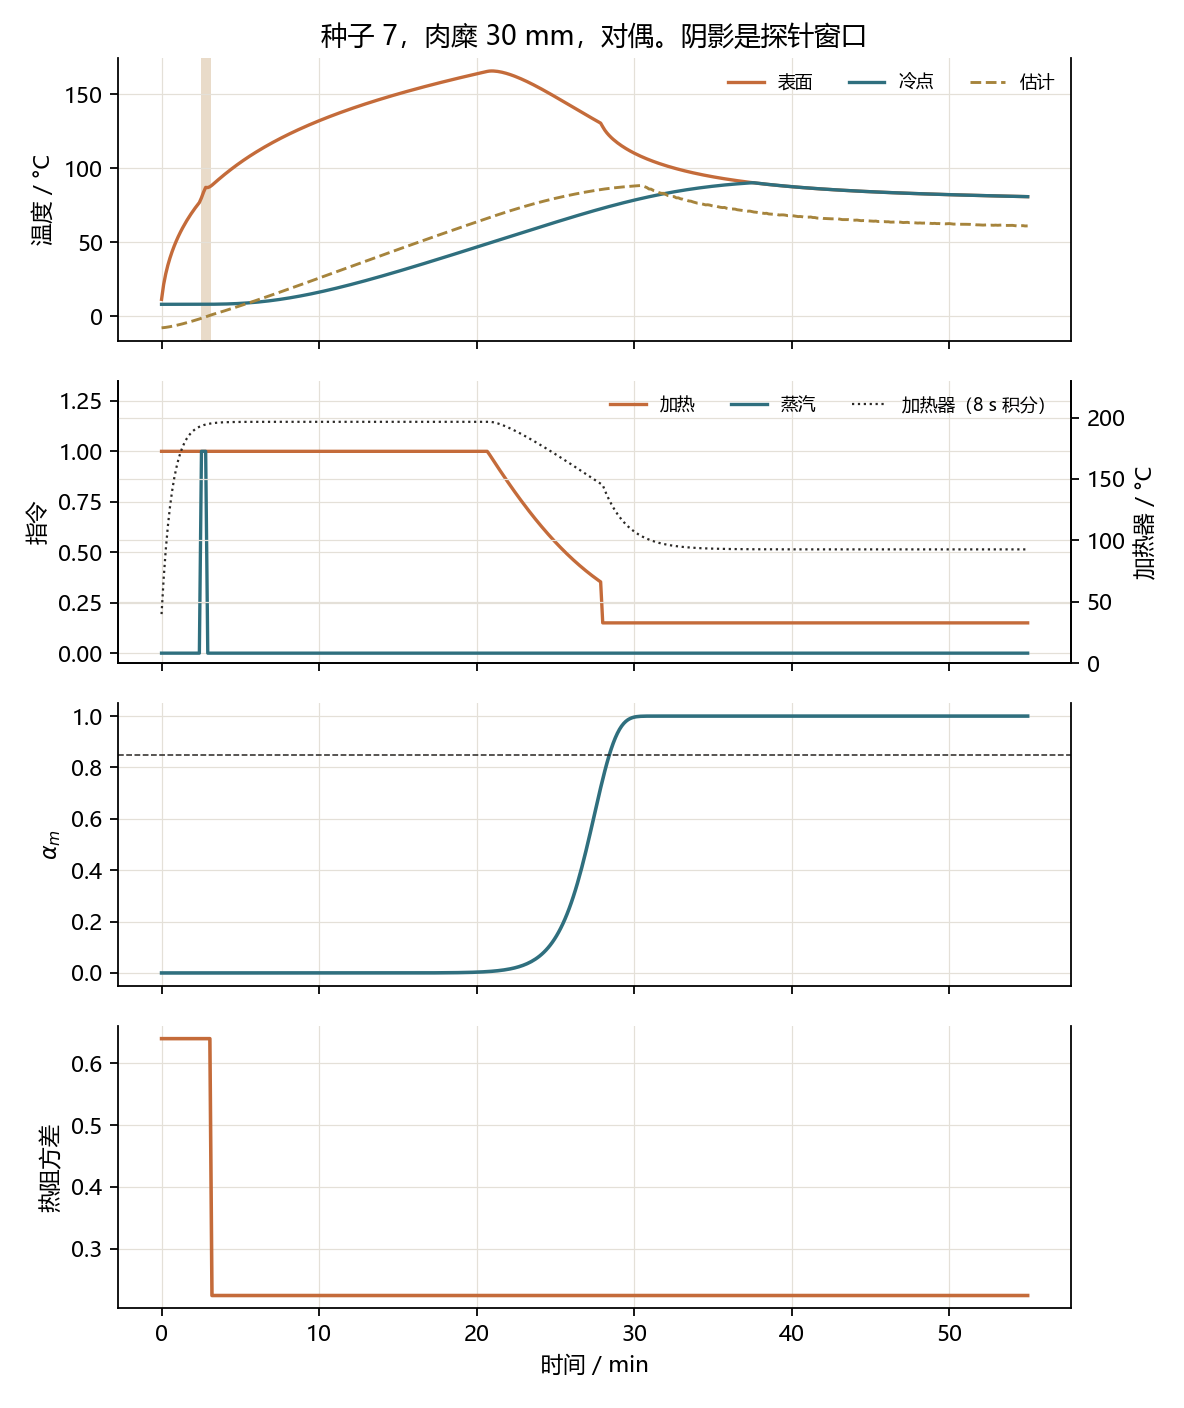
\includegraphics[width=\textwidth]{paper/P_seed7_panels.png}
\caption{种子 7 的四层记录。阴影是 150--190 s。加热器曲线用记录间隔 8 s 积分同一条加热指令，平衡仍是 \(196.5^\circ\mathrm{C}\)，不到 \(230^\circ\mathrm{C}\)。蒸汽脉冲在这张时间轴上只占很窄的一段。}
\end{figure}

\begin{figure}[ht]
\centering
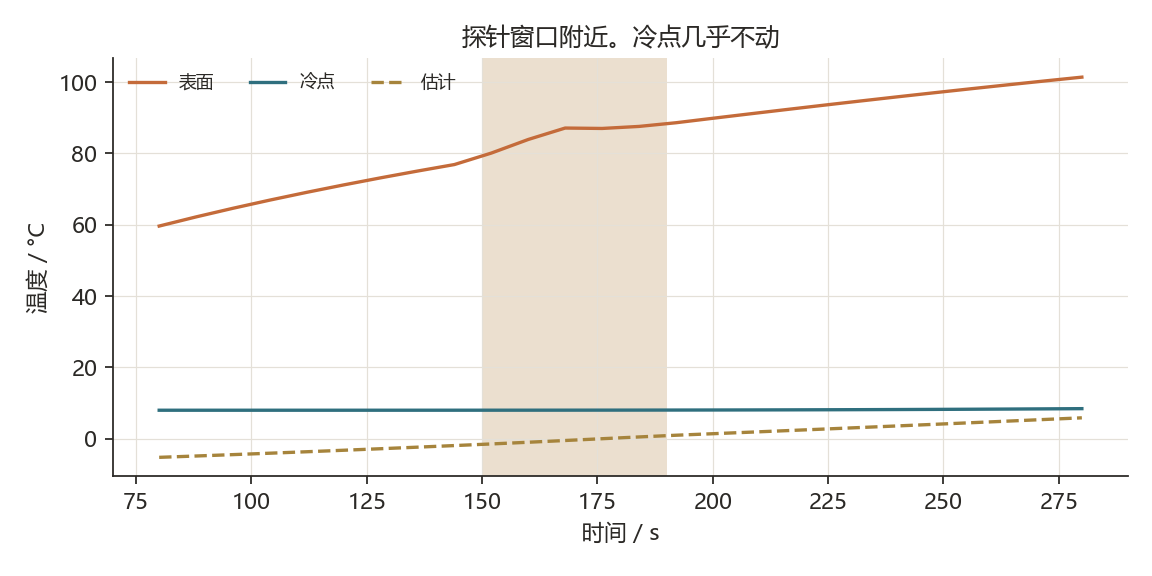
\includegraphics[width=0.92\textwidth]{paper/P_probe.png}
\caption{探针窗口附近。冷点保持在初温附近，表面已经升过 \(80^\circ\mathrm{C}\)。}
\end{figure}

\begin{figure}[ht]
\centering
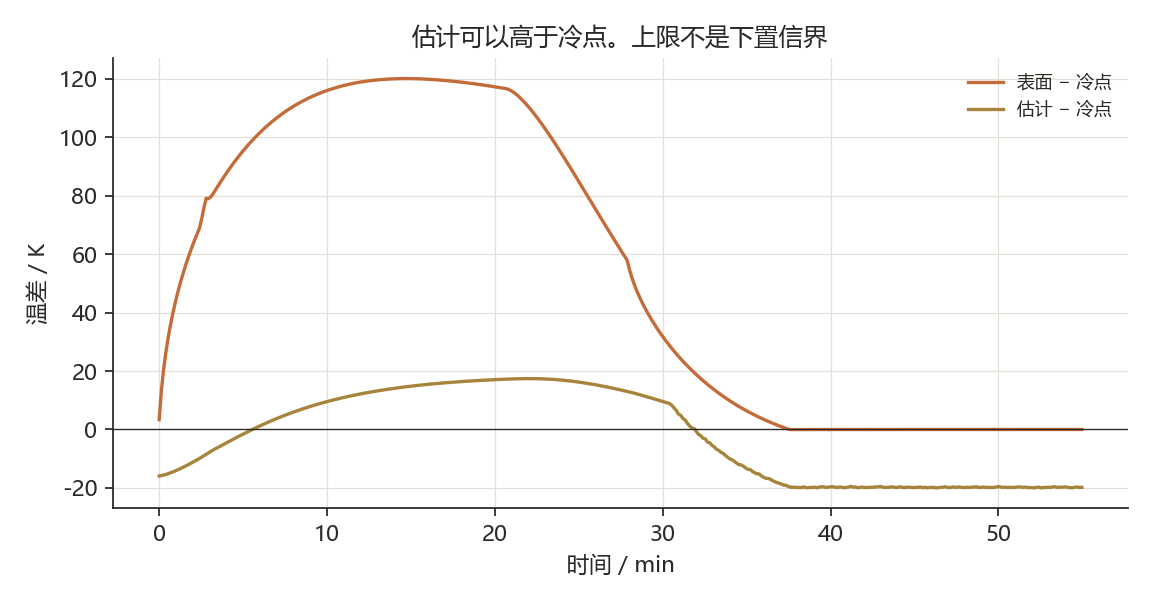
\includegraphics[width=0.92\textwidth]{paper/P_gap.png}
\caption{表面与冷点的温差，以及估计与冷点的温差。后一条曲线在中段为正，估计高于冷点。}
\end{figure}

\begin{figure}[ht]
\centering
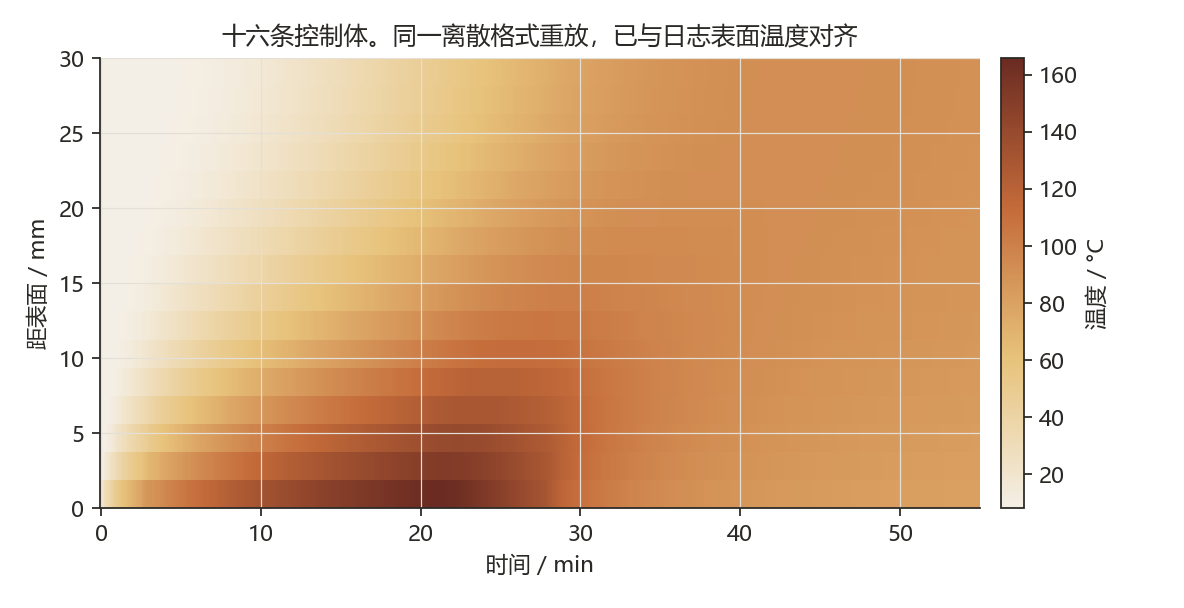
\includegraphics[width=\textwidth]{paper/P_field_xt.png}
\caption{重放得到的温度。纵轴是距表面的距离。高温区先出现在表面，冷点在深处，停机之后全厚度回落。这不是二维烤箱的切片。}
\end{figure}

\begin{figure}[ht]
\centering
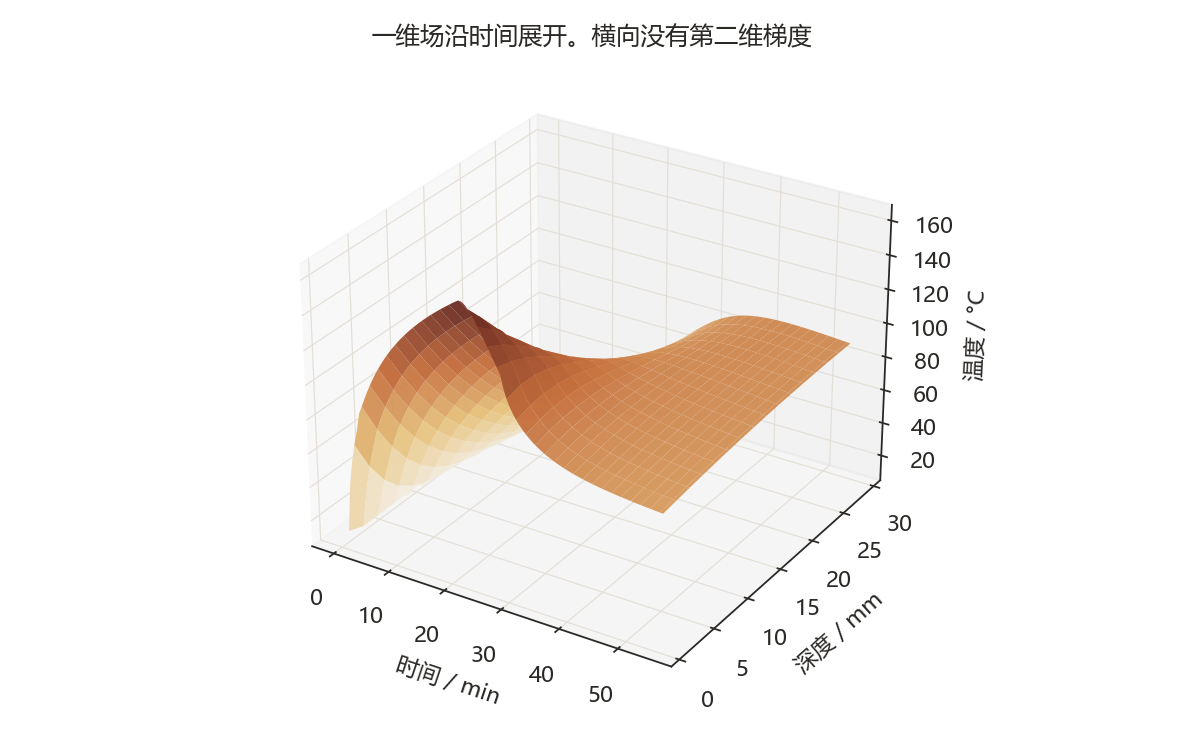
\includegraphics[width=0.88\textwidth]{paper/P_field_3d.png}
\caption{把同一条一维剖面沿时间立起来。深度轴上没有横向梯度，因为离散格式只有一个空间方向。}
\end{figure}

\begin{figure}[ht]
\centering
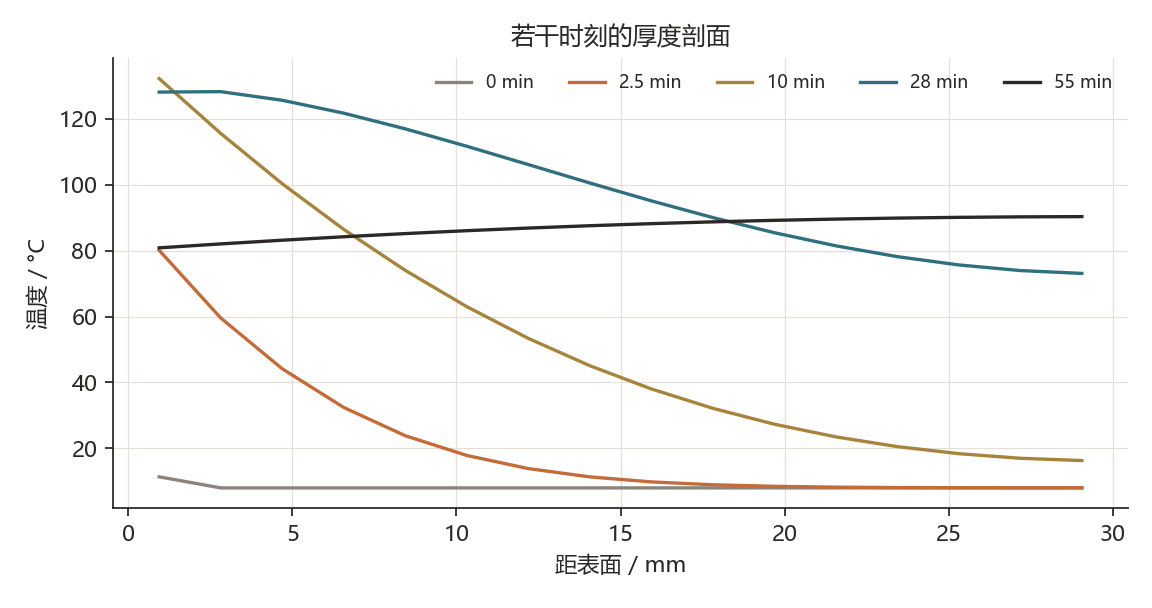
\includegraphics[width=0.9\textwidth]{paper/P_profiles.png}
\caption{0、2.5、10、28、55 min 的厚度剖面。2.5 min 时梯度集中在靠近表面的几个控制体。}
\end{figure}

\subsection{种子 7 的全部记录}
下表是 \texttt{demo\_seed7\_dual.csv} 的 414 行，记录间隔 8 s。表面温度是该步导热更新之后的值，冷点是更新之前十六个控制体的最低温度。估计冷点在观测器更新之后、导热更新之前写入。加热器温度不在这份 CSV 里。
\begin{longtable}{rrrrrrrr}
\caption{种子 7、对偶、肉糜 30 mm，全部记录}\\
\toprule
$t$ & 表面 & 冷点 & 估计 & $\alpha_m$ & 方差 & 加热 & 模式 \\
\midrule\endfirsthead
\toprule $t$ & 表面 & 冷点 & 估计 & $\alpha_m$ & 方差 & 加热 & 模式 \\\midrule\endhead
\bottomrule\endfoot
0 & 11.36 & 8.00 & -7.92 & 0.0000 & 0.640 & 1.000 & 品质 \\
8 & 21.45 & 8.00 & -7.79 & 0.0000 & 0.640 & 1.000 & 品质 \\
16 & 28.67 & 8.00 & -7.61 & 0.0000 & 0.640 & 1.000 & 品质 \\
24 & 34.43 & 8.00 & -7.39 & 0.0000 & 0.640 & 1.000 & 品质 \\
32 & 39.30 & 8.00 & -7.14 & 0.0000 & 0.640 & 1.000 & 品质 \\
40 & 43.55 & 8.00 & -6.86 & 0.0000 & 0.640 & 1.000 & 品质 \\
48 & 47.35 & 8.00 & -6.57 & 0.0000 & 0.640 & 1.000 & 品质 \\
56 & 50.80 & 8.00 & -6.25 & 0.0000 & 0.640 & 1.000 & 品质 \\
64 & 53.97 & 8.00 & -5.92 & 0.0000 & 0.640 & 1.000 & 品质 \\
72 & 56.90 & 8.00 & -5.57 & 0.0000 & 0.640 & 1.000 & 品质 \\
80 & 59.64 & 8.00 & -5.21 & 0.0000 & 0.640 & 1.000 & 品质 \\
88 & 62.20 & 8.00 & -4.83 & 0.0000 & 0.640 & 1.000 & 品质 \\
96 & 64.63 & 8.00 & -4.45 & 0.0000 & 0.640 & 1.000 & 品质 \\
104 & 66.92 & 8.00 & -4.05 & 0.0000 & 0.640 & 1.000 & 品质 \\
112 & 69.10 & 8.00 & -3.64 & 0.0000 & 0.640 & 1.000 & 品质 \\
120 & 71.17 & 8.00 & -3.22 & 0.0000 & 0.640 & 1.000 & 品质 \\
128 & 73.16 & 8.00 & -2.79 & 0.0000 & 0.640 & 1.000 & 品质 \\
136 & 75.06 & 8.00 & -2.36 & 0.0000 & 0.640 & 1.000 & 品质 \\
144 & 76.88 & 8.01 & -1.91 & 0.0000 & 0.640 & 1.000 & 品质 \\
152 & 80.10 & 8.01 & -1.45 & 0.0000 & 0.640 & 1.000 & 探针 \\
160 & 83.91 & 8.01 & -0.98 & 0.0000 & 0.640 & 1.000 & 探针 \\
168 & 87.12 & 8.02 & -0.49 & 0.0000 & 0.640 & 1.000 & 探针 \\
176 & 87.00 & 8.03 & 0.01 & 0.0000 & 0.640 & 1.000 & 探针 \\
184 & 87.57 & 8.04 & 0.51 & 0.0000 & 0.640 & 1.000 & 探针 \\
192 & 88.60 & 8.05 & 0.99 & 0.0000 & 0.224 & 1.000 & 品质 \\
200 & 89.85 & 8.06 & 1.41 & 0.0000 & 0.224 & 1.000 & 品质 \\
208 & 91.09 & 8.08 & 1.84 & 0.0000 & 0.224 & 1.000 & 品质 \\
216 & 92.31 & 8.10 & 2.28 & 0.0000 & 0.224 & 1.000 & 品质 \\
224 & 93.52 & 8.13 & 2.71 & 0.0000 & 0.224 & 1.000 & 品质 \\
232 & 94.70 & 8.16 & 3.15 & 0.0000 & 0.224 & 1.000 & 品质 \\
240 & 95.87 & 8.19 & 3.60 & 0.0000 & 0.224 & 1.000 & 品质 \\
248 & 97.01 & 8.23 & 4.05 & 0.0000 & 0.224 & 1.000 & 品质 \\
256 & 98.14 & 8.28 & 4.50 & 0.0000 & 0.224 & 1.000 & 品质 \\
264 & 99.24 & 8.33 & 4.95 & 0.0000 & 0.224 & 1.000 & 品质 \\
272 & 100.33 & 8.38 & 5.41 & 0.0000 & 0.224 & 1.000 & 品质 \\
280 & 101.39 & 8.44 & 5.87 & 0.0000 & 0.224 & 1.000 & 品质 \\
288 & 102.43 & 8.51 & 6.33 & 0.0000 & 0.224 & 1.000 & 品质 \\
296 & 103.45 & 8.58 & 6.80 & 0.0000 & 0.224 & 1.000 & 品质 \\
304 & 104.46 & 8.66 & 7.27 & 0.0000 & 0.224 & 1.000 & 品质 \\
312 & 105.44 & 8.75 & 7.74 & 0.0000 & 0.224 & 1.000 & 品质 \\
320 & 106.41 & 8.84 & 8.21 & 0.0000 & 0.224 & 1.000 & 品质 \\
328 & 107.36 & 8.94 & 8.69 & 0.0000 & 0.224 & 1.000 & 品质 \\
336 & 108.29 & 9.05 & 9.17 & 0.0000 & 0.224 & 1.000 & 品质 \\
344 & 109.21 & 9.16 & 9.65 & 0.0000 & 0.224 & 1.000 & 品质 \\
352 & 110.11 & 9.28 & 10.13 & 0.0000 & 0.224 & 1.000 & 品质 \\
360 & 111.00 & 9.40 & 10.62 & 0.0000 & 0.224 & 1.000 & 品质 \\
368 & 111.87 & 9.54 & 11.10 & 0.0000 & 0.224 & 1.000 & 品质 \\
376 & 112.72 & 9.68 & 11.59 & 0.0000 & 0.224 & 1.000 & 品质 \\
384 & 113.56 & 9.83 & 12.08 & 0.0000 & 0.224 & 1.000 & 品质 \\
392 & 114.39 & 9.98 & 12.58 & 0.0000 & 0.224 & 1.000 & 品质 \\
400 & 115.21 & 10.14 & 13.07 & 0.0000 & 0.224 & 1.000 & 品质 \\
408 & 116.01 & 10.31 & 13.56 & 0.0000 & 0.224 & 1.000 & 品质 \\
416 & 116.80 & 10.49 & 14.06 & 0.0000 & 0.224 & 1.000 & 品质 \\
424 & 117.58 & 10.67 & 14.56 & 0.0000 & 0.224 & 1.000 & 品质 \\
432 & 118.34 & 10.86 & 15.06 & 0.0000 & 0.224 & 1.000 & 品质 \\
440 & 119.10 & 11.05 & 15.56 & 0.0000 & 0.224 & 1.000 & 品质 \\
448 & 119.84 & 11.26 & 16.06 & 0.0000 & 0.224 & 1.000 & 品质 \\
456 & 120.57 & 11.47 & 16.56 & 0.0000 & 0.224 & 1.000 & 品质 \\
464 & 121.29 & 11.68 & 17.07 & 0.0000 & 0.224 & 1.000 & 品质 \\
472 & 122.01 & 11.90 & 17.57 & 0.0000 & 0.224 & 1.000 & 品质 \\
480 & 122.71 & 12.13 & 18.08 & 0.0000 & 0.224 & 1.000 & 品质 \\
488 & 123.40 & 12.36 & 18.59 & 0.0000 & 0.224 & 1.000 & 品质 \\
496 & 124.08 & 12.60 & 19.10 & 0.0000 & 0.224 & 1.000 & 品质 \\
504 & 124.76 & 12.85 & 19.61 & 0.0000 & 0.224 & 1.000 & 品质 \\
512 & 125.42 & 13.10 & 20.12 & 0.0000 & 0.224 & 1.000 & 品质 \\
520 & 126.08 & 13.36 & 20.63 & 0.0000 & 0.224 & 1.000 & 品质 \\
528 & 126.73 & 13.62 & 21.14 & 0.0000 & 0.224 & 1.000 & 品质 \\
536 & 127.37 & 13.89 & 21.65 & 0.0000 & 0.224 & 1.000 & 品质 \\
544 & 128.00 & 14.16 & 22.16 & 0.0000 & 0.224 & 1.000 & 品质 \\
552 & 128.63 & 14.44 & 22.67 & 0.0000 & 0.224 & 1.000 & 品质 \\
560 & 129.24 & 14.73 & 23.18 & 0.0000 & 0.224 & 1.000 & 品质 \\
568 & 129.85 & 15.02 & 23.70 & 0.0000 & 0.224 & 1.000 & 品质 \\
576 & 130.45 & 15.31 & 24.21 & 0.0000 & 0.224 & 1.000 & 品质 \\
584 & 131.05 & 15.61 & 24.73 & 0.0000 & 0.224 & 1.000 & 品质 \\
592 & 131.64 & 15.91 & 25.24 & 0.0000 & 0.224 & 1.000 & 品质 \\
600 & 132.22 & 16.22 & 25.76 & 0.0000 & 0.224 & 1.000 & 品质 \\
608 & 132.79 & 16.54 & 26.27 & 0.0000 & 0.224 & 1.000 & 品质 \\
616 & 133.36 & 16.85 & 26.79 & 0.0000 & 0.224 & 1.000 & 品质 \\
624 & 133.92 & 17.17 & 27.31 & 0.0000 & 0.224 & 1.000 & 品质 \\
632 & 134.48 & 17.50 & 27.82 & 0.0000 & 0.224 & 1.000 & 品质 \\
640 & 135.03 & 17.83 & 28.34 & 0.0000 & 0.224 & 1.000 & 品质 \\
648 & 135.57 & 18.17 & 28.86 & 0.0000 & 0.224 & 1.000 & 品质 \\
656 & 136.11 & 18.50 & 29.37 & 0.0000 & 0.224 & 1.000 & 品质 \\
664 & 136.64 & 18.85 & 29.89 & 0.0000 & 0.224 & 1.000 & 品质 \\
672 & 137.17 & 19.19 & 30.41 & 0.0000 & 0.224 & 1.000 & 品质 \\
680 & 137.69 & 19.54 & 30.93 & 0.0000 & 0.224 & 1.000 & 品质 \\
688 & 138.21 & 19.89 & 31.44 & 0.0000 & 0.224 & 1.000 & 品质 \\
696 & 138.72 & 20.25 & 31.96 & 0.0000 & 0.224 & 1.000 & 品质 \\
704 & 139.23 & 20.61 & 32.48 & 0.0000 & 0.224 & 1.000 & 品质 \\
712 & 139.73 & 20.97 & 32.99 & 0.0000 & 0.224 & 1.000 & 品质 \\
720 & 140.22 & 21.34 & 33.51 & 0.0000 & 0.224 & 1.000 & 品质 \\
728 & 140.72 & 21.71 & 34.03 & 0.0000 & 0.224 & 1.000 & 品质 \\
736 & 141.20 & 22.08 & 34.54 & 0.0000 & 0.224 & 1.000 & 品质 \\
744 & 141.69 & 22.46 & 35.06 & 0.0000 & 0.224 & 1.000 & 品质 \\
752 & 142.16 & 22.84 & 35.58 & 0.0000 & 0.224 & 1.000 & 品质 \\
760 & 142.64 & 23.22 & 36.09 & 0.0000 & 0.224 & 1.000 & 品质 \\
768 & 143.11 & 23.60 & 36.61 & 0.0000 & 0.224 & 1.000 & 品质 \\
776 & 143.57 & 23.99 & 37.12 & 0.0000 & 0.224 & 1.000 & 品质 \\
784 & 144.03 & 24.38 & 37.64 & 0.0000 & 0.224 & 1.000 & 品质 \\
792 & 144.49 & 24.77 & 38.15 & 0.0000 & 0.224 & 1.000 & 品质 \\
800 & 144.95 & 25.16 & 38.67 & 0.0000 & 0.224 & 1.000 & 品质 \\
808 & 145.40 & 25.56 & 39.18 & 0.0000 & 0.224 & 1.000 & 品质 \\
816 & 145.84 & 25.96 & 39.70 & 0.0000 & 0.224 & 1.000 & 品质 \\
824 & 146.28 & 26.36 & 40.21 & 0.0000 & 0.224 & 1.000 & 品质 \\
832 & 146.72 & 26.76 & 40.73 & 0.0000 & 0.224 & 1.000 & 品质 \\
840 & 147.16 & 27.17 & 41.24 & 0.0000 & 0.224 & 1.000 & 品质 \\
848 & 147.59 & 27.57 & 41.75 & 0.0001 & 0.224 & 1.000 & 品质 \\
856 & 148.02 & 27.98 & 42.26 & 0.0001 & 0.224 & 1.000 & 品质 \\
864 & 148.44 & 28.39 & 42.78 & 0.0001 & 0.224 & 1.000 & 品质 \\
872 & 148.86 & 28.81 & 43.29 & 0.0001 & 0.224 & 1.000 & 品质 \\
880 & 149.28 & 29.22 & 43.80 & 0.0001 & 0.224 & 1.000 & 品质 \\
888 & 149.70 & 29.64 & 44.31 & 0.0001 & 0.224 & 1.000 & 品质 \\
896 & 150.11 & 30.06 & 44.82 & 0.0001 & 0.224 & 1.000 & 品质 \\
904 & 150.52 & 30.48 & 45.33 & 0.0001 & 0.224 & 1.000 & 品质 \\
912 & 150.93 & 30.90 & 45.84 & 0.0001 & 0.224 & 1.000 & 品质 \\
920 & 151.33 & 31.32 & 46.35 & 0.0001 & 0.224 & 1.000 & 品质 \\
928 & 151.73 & 31.74 & 46.86 & 0.0001 & 0.224 & 1.000 & 品质 \\
936 & 152.13 & 32.17 & 47.36 & 0.0001 & 0.224 & 1.000 & 品质 \\
944 & 152.52 & 32.60 & 47.87 & 0.0001 & 0.224 & 1.000 & 品质 \\
952 & 152.91 & 33.02 & 48.38 & 0.0001 & 0.224 & 1.000 & 品质 \\
960 & 153.30 & 33.45 & 48.88 & 0.0002 & 0.224 & 1.000 & 品质 \\
968 & 153.69 & 33.88 & 49.39 & 0.0002 & 0.224 & 1.000 & 品质 \\
976 & 154.08 & 34.32 & 49.89 & 0.0002 & 0.224 & 1.000 & 品质 \\
984 & 154.46 & 34.75 & 50.40 & 0.0002 & 0.224 & 1.000 & 品质 \\
992 & 154.84 & 35.18 & 50.90 & 0.0002 & 0.224 & 1.000 & 品质 \\
1000 & 155.21 & 35.62 & 51.40 & 0.0003 & 0.224 & 1.000 & 品质 \\
1008 & 155.59 & 36.05 & 51.91 & 0.0003 & 0.224 & 1.000 & 品质 \\
1016 & 155.96 & 36.49 & 52.41 & 0.0003 & 0.224 & 1.000 & 品质 \\
1024 & 156.33 & 36.93 & 52.91 & 0.0003 & 0.224 & 1.000 & 品质 \\
1032 & 156.70 & 37.37 & 53.41 & 0.0004 & 0.224 & 1.000 & 品质 \\
1040 & 157.06 & 37.81 & 53.91 & 0.0004 & 0.224 & 1.000 & 品质 \\
1048 & 157.43 & 38.25 & 54.41 & 0.0005 & 0.224 & 1.000 & 品质 \\
1056 & 157.79 & 38.69 & 54.91 & 0.0005 & 0.224 & 1.000 & 品质 \\
1064 & 158.15 & 39.13 & 55.40 & 0.0006 & 0.224 & 1.000 & 品质 \\
1072 & 158.51 & 39.57 & 55.90 & 0.0006 & 0.224 & 1.000 & 品质 \\
1080 & 158.86 & 40.01 & 56.40 & 0.0007 & 0.224 & 1.000 & 品质 \\
1088 & 159.21 & 40.46 & 56.89 & 0.0008 & 0.224 & 1.000 & 品质 \\
1096 & 159.57 & 40.90 & 57.39 & 0.0008 & 0.224 & 1.000 & 品质 \\
1104 & 159.91 & 41.35 & 57.88 & 0.0009 & 0.224 & 1.000 & 品质 \\
1112 & 160.26 & 41.79 & 58.38 & 0.0010 & 0.224 & 1.000 & 品质 \\
1120 & 160.61 & 42.24 & 58.87 & 0.0011 & 0.224 & 1.000 & 品质 \\
1128 & 160.95 & 42.68 & 59.36 & 0.0012 & 0.224 & 1.000 & 品质 \\
1136 & 161.29 & 43.13 & 59.86 & 0.0014 & 0.224 & 1.000 & 品质 \\
1144 & 161.63 & 43.58 & 60.35 & 0.0015 & 0.224 & 1.000 & 品质 \\
1152 & 161.97 & 44.03 & 60.84 & 0.0017 & 0.224 & 1.000 & 品质 \\
1160 & 162.31 & 44.47 & 61.33 & 0.0019 & 0.224 & 1.000 & 品质 \\
1168 & 162.64 & 44.92 & 61.81 & 0.0021 & 0.224 & 1.000 & 品质 \\
1176 & 162.98 & 45.37 & 62.30 & 0.0023 & 0.224 & 1.000 & 品质 \\
1184 & 163.31 & 45.82 & 62.79 & 0.0025 & 0.224 & 1.000 & 品质 \\
1192 & 163.64 & 46.27 & 63.28 & 0.0028 & 0.224 & 1.000 & 品质 \\
1200 & 163.97 & 46.72 & 63.76 & 0.0031 & 0.224 & 1.000 & 品质 \\
1208 & 164.29 & 47.17 & 64.25 & 0.0034 & 0.224 & 1.000 & 品质 \\
1216 & 164.62 & 47.62 & 64.73 & 0.0038 & 0.224 & 1.000 & 品质 \\
1224 & 164.94 & 48.07 & 65.22 & 0.0042 & 0.224 & 1.000 & 品质 \\
1232 & 165.27 & 48.52 & 65.70 & 0.0047 & 0.224 & 1.000 & 品质 \\
1240 & 165.59 & 48.97 & 66.18 & 0.0052 & 0.224 & 1.000 & 品质 \\
1248 & 165.81 & 49.42 & 66.66 & 0.0057 & 0.224 & 0.986 & 品质 \\
1256 & 165.89 & 49.87 & 67.14 & 0.0063 & 0.224 & 0.970 & 品质 \\
1264 & 165.87 & 50.32 & 67.62 & 0.0070 & 0.224 & 0.954 & 品质 \\
1272 & 165.76 & 50.77 & 68.09 & 0.0078 & 0.224 & 0.938 & 品质 \\
1280 & 165.58 & 51.22 & 68.56 & 0.0086 & 0.224 & 0.922 & 品质 \\
1288 & 165.35 & 51.67 & 69.03 & 0.0096 & 0.224 & 0.907 & 品质 \\
1296 & 165.05 & 52.12 & 69.50 & 0.0106 & 0.224 & 0.891 & 品质 \\
1304 & 164.71 & 52.57 & 69.96 & 0.0118 & 0.224 & 0.876 & 品质 \\
1312 & 164.32 & 53.02 & 70.42 & 0.0130 & 0.224 & 0.861 & 品质 \\
1320 & 163.89 & 53.47 & 70.87 & 0.0144 & 0.224 & 0.845 & 品质 \\
1328 & 163.43 & 53.92 & 71.32 & 0.0160 & 0.224 & 0.830 & 品质 \\
1336 & 162.93 & 54.37 & 71.76 & 0.0177 & 0.224 & 0.816 & 品质 \\
1344 & 162.40 & 54.82 & 72.20 & 0.0196 & 0.224 & 0.801 & 品质 \\
1352 & 161.84 & 55.27 & 72.64 & 0.0217 & 0.224 & 0.787 & 品质 \\
1360 & 161.26 & 55.72 & 73.07 & 0.0241 & 0.224 & 0.772 & 品质 \\
1368 & 160.65 & 56.17 & 73.49 & 0.0267 & 0.224 & 0.758 & 品质 \\
1376 & 160.02 & 56.62 & 73.91 & 0.0295 & 0.224 & 0.744 & 品质 \\
1384 & 159.36 & 57.07 & 74.33 & 0.0327 & 0.224 & 0.730 & 品质 \\
1392 & 158.69 & 57.52 & 74.74 & 0.0362 & 0.224 & 0.716 & 品质 \\
1400 & 158.00 & 57.97 & 75.14 & 0.0401 & 0.224 & 0.703 & 品质 \\
1408 & 157.29 & 58.41 & 75.54 & 0.0443 & 0.224 & 0.690 & 品质 \\
1416 & 156.57 & 58.86 & 75.94 & 0.0490 & 0.224 & 0.677 & 品质 \\
1424 & 155.84 & 59.31 & 76.32 & 0.0542 & 0.224 & 0.664 & 品质 \\
1432 & 155.09 & 59.76 & 76.71 & 0.0599 & 0.224 & 0.651 & 品质 \\
1440 & 154.33 & 60.20 & 77.08 & 0.0662 & 0.224 & 0.638 & 品质 \\
1448 & 153.56 & 60.65 & 77.46 & 0.0732 & 0.224 & 0.626 & 品质 \\
1456 & 152.78 & 61.09 & 77.82 & 0.0808 & 0.224 & 0.614 & 品质 \\
1464 & 151.99 & 61.54 & 78.18 & 0.0892 & 0.224 & 0.602 & 品质 \\
1472 & 151.19 & 61.98 & 78.54 & 0.0983 & 0.224 & 0.590 & 品质 \\
1480 & 150.39 & 62.43 & 78.89 & 0.1084 & 0.224 & 0.578 & 品质 \\
1488 & 149.58 & 62.87 & 79.24 & 0.1194 & 0.224 & 0.567 & 品质 \\
1496 & 148.76 & 63.31 & 79.57 & 0.1315 & 0.224 & 0.555 & 品质 \\
1504 & 147.94 & 63.75 & 79.91 & 0.1446 & 0.224 & 0.544 & 品质 \\
1512 & 147.11 & 64.19 & 80.23 & 0.1589 & 0.224 & 0.533 & 品质 \\
1520 & 146.29 & 64.63 & 80.56 & 0.1744 & 0.224 & 0.523 & 品质 \\
1528 & 145.46 & 65.07 & 80.87 & 0.1913 & 0.224 & 0.512 & 品质 \\
1536 & 144.62 & 65.50 & 81.18 & 0.2095 & 0.224 & 0.502 & 品质 \\
1544 & 143.79 & 65.94 & 81.49 & 0.2292 & 0.224 & 0.491 & 品质 \\
1552 & 142.95 & 66.37 & 81.79 & 0.2504 & 0.224 & 0.482 & 品质 \\
1560 & 142.12 & 66.80 & 82.08 & 0.2731 & 0.224 & 0.472 & 品质 \\
1568 & 141.28 & 67.23 & 82.37 & 0.2973 & 0.224 & 0.462 & 品质 \\
1576 & 140.45 & 67.66 & 82.65 & 0.3232 & 0.224 & 0.453 & 品质 \\
1584 & 139.61 & 68.08 & 82.93 & 0.3506 & 0.224 & 0.443 & 品质 \\
1592 & 138.78 & 68.50 & 83.20 & 0.3795 & 0.224 & 0.434 & 品质 \\
1600 & 137.95 & 68.93 & 83.47 & 0.4099 & 0.224 & 0.425 & 品质 \\
1608 & 137.12 & 69.34 & 83.73 & 0.4416 & 0.224 & 0.417 & 品质 \\
1616 & 136.29 & 69.76 & 83.99 & 0.4746 & 0.224 & 0.408 & 品质 \\
1624 & 135.47 & 70.18 & 84.24 & 0.5087 & 0.224 & 0.400 & 品质 \\
1632 & 134.64 & 70.59 & 84.49 & 0.5436 & 0.224 & 0.392 & 品质 \\
1640 & 133.83 & 71.00 & 84.73 & 0.5791 & 0.224 & 0.384 & 品质 \\
1648 & 133.01 & 71.40 & 84.96 & 0.6149 & 0.224 & 0.376 & 品质 \\
1656 & 132.21 & 71.80 & 85.19 & 0.6507 & 0.224 & 0.368 & 品质 \\
1664 & 131.40 & 72.21 & 85.42 & 0.6862 & 0.224 & 0.360 & 品质 \\
1672 & 130.60 & 72.60 & 85.64 & 0.7209 & 0.224 & 0.353 & 品质 \\
1680 & 128.12 & 73.00 & 85.85 & 0.7546 & 0.224 & 0.150 & 保持 \\
1688 & 125.82 & 73.39 & 86.05 & 0.7868 & 0.224 & 0.150 & 保持 \\
1696 & 123.96 & 73.78 & 86.24 & 0.8172 & 0.224 & 0.150 & 保持 \\
1704 & 122.34 & 74.16 & 86.42 & 0.8455 & 0.224 & 0.150 & 保持 \\
1712 & 120.91 & 74.54 & 86.59 & 0.8714 & 0.224 & 0.150 & 保持 \\
1720 & 119.60 & 74.92 & 86.76 & 0.8948 & 0.224 & 0.150 & 保持 \\
1728 & 118.40 & 75.30 & 86.91 & 0.9154 & 0.224 & 0.150 & 保持 \\
1736 & 117.28 & 75.67 & 87.06 & 0.9334 & 0.224 & 0.150 & 保持 \\
1744 & 116.24 & 76.03 & 87.21 & 0.9486 & 0.224 & 0.150 & 保持 \\
1752 & 115.25 & 76.40 & 87.35 & 0.9612 & 0.224 & 0.150 & 保持 \\
1760 & 114.32 & 76.76 & 87.48 & 0.9715 & 0.224 & 0.150 & 保持 \\
1768 & 113.43 & 77.12 & 87.61 & 0.9795 & 0.224 & 0.150 & 保持 \\
1776 & 112.59 & 77.47 & 87.73 & 0.9857 & 0.224 & 0.150 & 保持 \\
1784 & 111.79 & 77.82 & 87.85 & 0.9904 & 0.224 & 0.150 & 保持 \\
1792 & 111.02 & 78.16 & 87.96 & 0.9937 & 0.224 & 0.150 & 保持 \\
1800 & 110.28 & 78.50 & 88.07 & 0.9960 & 0.224 & 0.150 & 保持 \\
1808 & 109.57 & 78.84 & 88.18 & 0.9976 & 0.224 & 0.150 & 保持 \\
1816 & 108.89 & 79.17 & 88.28 & 0.9986 & 0.224 & 0.150 & 保持 \\
1824 & 108.23 & 79.50 & 88.38 & 0.9992 & 0.224 & 0.150 & 保持 \\
1832 & 107.60 & 79.82 & 88.14 & 0.9996 & 0.224 & 0.150 & 保持 \\
1840 & 106.99 & 80.14 & 87.55 & 0.9998 & 0.224 & 0.150 & 保持 \\
1848 & 106.39 & 80.46 & 87.01 & 0.9999 & 0.224 & 0.150 & 保持 \\
1856 & 105.82 & 80.77 & 86.03 & 1.0000 & 0.224 & 0.150 & 保持 \\
1864 & 105.27 & 81.08 & 85.94 & 1.0000 & 0.224 & 0.150 & 保持 \\
1872 & 104.73 & 81.38 & 85.14 & 1.0000 & 0.224 & 0.150 & 保持 \\
1880 & 104.22 & 81.67 & 84.90 & 1.0000 & 0.224 & 0.150 & 保持 \\
1888 & 103.71 & 81.97 & 84.04 & 1.0000 & 0.224 & 0.150 & 保持 \\
1896 & 103.22 & 82.25 & 83.45 & 1.0000 & 0.224 & 0.150 & 保持 \\
1904 & 102.75 & 82.54 & 83.08 & 1.0000 & 0.224 & 0.150 & 保持 \\
1912 & 102.29 & 82.81 & 83.12 & 1.0000 & 0.224 & 0.150 & 保持 \\
1920 & 101.84 & 83.09 & 82.39 & 1.0000 & 0.224 & 0.150 & 保持 \\
1928 & 101.40 & 83.35 & 81.59 & 1.0000 & 0.224 & 0.150 & 保持 \\
1936 & 100.98 & 83.62 & 81.46 & 1.0000 & 0.224 & 0.150 & 保持 \\
1944 & 100.57 & 83.87 & 80.87 & 1.0000 & 0.224 & 0.150 & 保持 \\
1952 & 100.16 & 84.13 & 80.87 & 1.0000 & 0.224 & 0.150 & 保持 \\
1960 & 99.77 & 84.37 & 80.04 & 1.0000 & 0.224 & 0.150 & 保持 \\
1968 & 99.39 & 84.62 & 80.04 & 1.0000 & 0.224 & 0.150 & 保持 \\
1976 & 99.02 & 84.85 & 79.41 & 1.0000 & 0.224 & 0.150 & 保持 \\
1984 & 98.66 & 85.09 & 79.13 & 1.0000 & 0.224 & 0.150 & 保持 \\
1992 & 98.30 & 85.31 & 78.55 & 1.0000 & 0.224 & 0.150 & 保持 \\
2000 & 97.96 & 85.54 & 78.36 & 1.0000 & 0.224 & 0.150 & 保持 \\
2008 & 97.62 & 85.75 & 77.93 & 1.0000 & 0.224 & 0.150 & 保持 \\
2016 & 97.29 & 85.97 & 77.78 & 1.0000 & 0.224 & 0.150 & 保持 \\
2024 & 96.97 & 86.17 & 77.27 & 1.0000 & 0.224 & 0.150 & 保持 \\
2032 & 96.66 & 86.38 & 76.85 & 1.0000 & 0.224 & 0.150 & 保持 \\
2040 & 96.35 & 86.58 & 76.47 & 1.0000 & 0.224 & 0.150 & 保持 \\
2048 & 96.05 & 86.77 & 76.40 & 1.0000 & 0.224 & 0.150 & 保持 \\
2056 & 95.76 & 86.96 & 76.00 & 1.0000 & 0.224 & 0.150 & 保持 \\
2064 & 95.48 & 87.14 & 75.65 & 1.0000 & 0.224 & 0.150 & 保持 \\
2072 & 95.20 & 87.32 & 75.27 & 1.0000 & 0.224 & 0.150 & 保持 \\
2080 & 94.92 & 87.50 & 75.37 & 1.0000 & 0.224 & 0.150 & 保持 \\
2088 & 94.66 & 87.67 & 75.12 & 1.0000 & 0.224 & 0.150 & 保持 \\
2096 & 94.39 & 87.83 & 74.68 & 1.0000 & 0.224 & 0.150 & 保持 \\
2104 & 94.14 & 88.00 & 74.36 & 1.0000 & 0.224 & 0.150 & 保持 \\
2112 & 93.89 & 88.15 & 74.45 & 1.0000 & 0.224 & 0.150 & 保持 \\
2120 & 93.64 & 88.31 & 73.99 & 1.0000 & 0.224 & 0.150 & 保持 \\
2128 & 93.41 & 88.46 & 73.65 & 1.0000 & 0.224 & 0.150 & 保持 \\
2136 & 93.17 & 88.60 & 73.46 & 1.0000 & 0.224 & 0.150 & 保持 \\
2144 & 92.94 & 88.74 & 73.54 & 1.0000 & 0.224 & 0.150 & 保持 \\
2152 & 92.72 & 88.88 & 72.98 & 1.0000 & 0.224 & 0.150 & 保持 \\
2160 & 92.50 & 89.01 & 72.69 & 1.0000 & 0.224 & 0.150 & 保持 \\
2168 & 92.28 & 89.14 & 72.43 & 1.0000 & 0.224 & 0.150 & 保持 \\
2176 & 92.07 & 89.27 & 72.51 & 1.0000 & 0.224 & 0.150 & 保持 \\
2184 & 91.86 & 89.39 & 72.42 & 1.0000 & 0.224 & 0.150 & 保持 \\
2192 & 91.66 & 89.51 & 72.00 & 1.0000 & 0.224 & 0.150 & 保持 \\
2200 & 91.46 & 89.63 & 71.79 & 1.0000 & 0.224 & 0.150 & 保持 \\
2208 & 91.27 & 89.74 & 71.55 & 1.0000 & 0.224 & 0.150 & 保持 \\
2216 & 91.08 & 89.85 & 71.45 & 1.0000 & 0.224 & 0.150 & 保持 \\
2224 & 90.89 & 89.95 & 71.25 & 1.0000 & 0.224 & 0.150 & 保持 \\
2232 & 90.71 & 90.05 & 71.02 & 1.0000 & 0.224 & 0.150 & 保持 \\
2240 & 90.53 & 90.15 & 71.08 & 1.0000 & 0.224 & 0.150 & 保持 \\
2248 & 90.35 & 90.25 & 70.77 & 1.0000 & 0.224 & 0.150 & 保持 \\
2256 & 90.18 & 90.22 & 70.44 & 1.0000 & 0.224 & 0.150 & 保持 \\
2264 & 90.01 & 90.05 & 70.31 & 1.0000 & 0.224 & 0.150 & 保持 \\
2272 & 89.85 & 89.89 & 70.04 & 1.0000 & 0.224 & 0.150 & 保持 \\
2280 & 89.68 & 89.72 & 69.93 & 1.0000 & 0.224 & 0.150 & 保持 \\
2288 & 89.52 & 89.56 & 69.73 & 1.0000 & 0.224 & 0.150 & 保持 \\
2296 & 89.37 & 89.40 & 69.51 & 1.0000 & 0.224 & 0.150 & 保持 \\
2304 & 89.21 & 89.25 & 69.60 & 1.0000 & 0.224 & 0.150 & 保持 \\
2312 & 89.06 & 89.10 & 69.14 & 1.0000 & 0.224 & 0.150 & 保持 \\
2320 & 88.91 & 88.95 & 69.06 & 1.0000 & 0.224 & 0.150 & 保持 \\
2328 & 88.77 & 88.80 & 68.95 & 1.0000 & 0.224 & 0.150 & 保持 \\
2336 & 88.63 & 88.66 & 68.80 & 1.0000 & 0.224 & 0.150 & 保持 \\
2344 & 88.49 & 88.52 & 68.76 & 1.0000 & 0.224 & 0.150 & 保持 \\
2352 & 88.35 & 88.38 & 68.42 & 1.0000 & 0.224 & 0.150 & 保持 \\
2360 & 88.21 & 88.25 & 68.52 & 1.0000 & 0.224 & 0.150 & 保持 \\
2368 & 88.08 & 88.11 & 68.51 & 1.0000 & 0.224 & 0.150 & 保持 \\
2376 & 87.95 & 87.98 & 68.32 & 1.0000 & 0.224 & 0.150 & 保持 \\
2384 & 87.82 & 87.86 & 68.00 & 1.0000 & 0.224 & 0.150 & 保持 \\
2392 & 87.70 & 87.73 & 68.00 & 1.0000 & 0.224 & 0.150 & 保持 \\
2400 & 87.57 & 87.61 & 67.98 & 1.0000 & 0.224 & 0.150 & 保持 \\
2408 & 87.45 & 87.48 & 67.84 & 1.0000 & 0.224 & 0.150 & 保持 \\
2416 & 87.33 & 87.36 & 67.59 & 1.0000 & 0.224 & 0.150 & 保持 \\
2424 & 87.22 & 87.25 & 67.37 & 1.0000 & 0.224 & 0.150 & 保持 \\
2432 & 87.10 & 87.13 & 67.44 & 1.0000 & 0.224 & 0.150 & 保持 \\
2440 & 86.99 & 87.02 & 67.25 & 1.0000 & 0.224 & 0.150 & 保持 \\
2448 & 86.88 & 86.91 & 66.97 & 1.0000 & 0.224 & 0.150 & 保持 \\
2456 & 86.77 & 86.80 & 66.95 & 1.0000 & 0.224 & 0.150 & 保持 \\
2464 & 86.66 & 86.69 & 66.99 & 1.0000 & 0.224 & 0.150 & 保持 \\
2472 & 86.56 & 86.58 & 67.09 & 1.0000 & 0.224 & 0.150 & 保持 \\
2480 & 86.45 & 86.48 & 66.74 & 1.0000 & 0.224 & 0.150 & 保持 \\
2488 & 86.35 & 86.38 & 66.70 & 1.0000 & 0.224 & 0.150 & 保持 \\
2496 & 86.25 & 86.28 & 66.35 & 1.0000 & 0.224 & 0.150 & 保持 \\
2504 & 86.15 & 86.18 & 66.29 & 1.0000 & 0.224 & 0.150 & 保持 \\
2512 & 86.06 & 86.08 & 66.39 & 1.0000 & 0.224 & 0.150 & 保持 \\
2520 & 85.96 & 85.99 & 66.12 & 1.0000 & 0.224 & 0.150 & 保持 \\
2528 & 85.87 & 85.89 & 66.04 & 1.0000 & 0.224 & 0.150 & 保持 \\
2536 & 85.78 & 85.80 & 65.92 & 1.0000 & 0.224 & 0.150 & 保持 \\
2544 & 85.69 & 85.71 & 65.91 & 1.0000 & 0.224 & 0.150 & 保持 \\
2552 & 85.60 & 85.62 & 65.85 & 1.0000 & 0.224 & 0.150 & 保持 \\
2560 & 85.51 & 85.53 & 65.85 & 1.0000 & 0.224 & 0.150 & 保持 \\
2568 & 85.42 & 85.44 & 65.75 & 1.0000 & 0.224 & 0.150 & 保持 \\
2576 & 85.34 & 85.36 & 65.85 & 1.0000 & 0.224 & 0.150 & 保持 \\
2584 & 85.25 & 85.27 & 65.58 & 1.0000 & 0.224 & 0.150 & 保持 \\
2592 & 85.17 & 85.19 & 65.33 & 1.0000 & 0.224 & 0.150 & 保持 \\
2600 & 85.09 & 85.11 & 65.30 & 1.0000 & 0.224 & 0.150 & 保持 \\
2608 & 85.01 & 85.03 & 65.22 & 1.0000 & 0.224 & 0.150 & 保持 \\
2616 & 84.93 & 84.95 & 65.31 & 1.0000 & 0.224 & 0.150 & 保持 \\
2624 & 84.85 & 84.87 & 65.11 & 1.0000 & 0.224 & 0.150 & 保持 \\
2632 & 84.78 & 84.80 & 64.95 & 1.0000 & 0.224 & 0.150 & 保持 \\
2640 & 84.70 & 84.72 & 64.92 & 1.0000 & 0.224 & 0.150 & 保持 \\
2648 & 84.63 & 84.65 & 65.01 & 1.0000 & 0.224 & 0.150 & 保持 \\
2656 & 84.56 & 84.57 & 64.78 & 1.0000 & 0.224 & 0.150 & 保持 \\
2664 & 84.48 & 84.50 & 64.58 & 1.0000 & 0.224 & 0.150 & 保持 \\
2672 & 84.41 & 84.43 & 64.68 & 1.0000 & 0.224 & 0.150 & 保持 \\
2680 & 84.34 & 84.36 & 64.59 & 1.0000 & 0.224 & 0.150 & 保持 \\
2688 & 84.27 & 84.29 & 64.47 & 1.0000 & 0.224 & 0.150 & 保持 \\
2696 & 84.21 & 84.22 & 64.35 & 1.0000 & 0.224 & 0.150 & 保持 \\
2704 & 84.14 & 84.16 & 64.31 & 1.0000 & 0.224 & 0.150 & 保持 \\
2712 & 84.07 & 84.09 & 64.24 & 1.0000 & 0.224 & 0.150 & 保持 \\
2720 & 84.01 & 84.02 & 64.33 & 1.0000 & 0.224 & 0.150 & 保持 \\
2728 & 83.94 & 83.96 & 64.02 & 1.0000 & 0.224 & 0.150 & 保持 \\
2736 & 83.88 & 83.90 & 64.11 & 1.0000 & 0.224 & 0.150 & 保持 \\
2744 & 83.82 & 83.83 & 63.88 & 1.0000 & 0.224 & 0.150 & 保持 \\
2752 & 83.76 & 83.77 & 63.94 & 1.0000 & 0.224 & 0.150 & 保持 \\
2760 & 83.70 & 83.71 & 63.85 & 1.0000 & 0.224 & 0.150 & 保持 \\
2768 & 83.64 & 83.65 & 63.85 & 1.0000 & 0.224 & 0.150 & 保持 \\
2776 & 83.58 & 83.59 & 63.60 & 1.0000 & 0.224 & 0.150 & 保持 \\
2784 & 83.52 & 83.53 & 63.62 & 1.0000 & 0.224 & 0.150 & 保持 \\
2792 & 83.46 & 83.48 & 63.62 & 1.0000 & 0.224 & 0.150 & 保持 \\
2800 & 83.40 & 83.42 & 63.65 & 1.0000 & 0.224 & 0.150 & 保持 \\
2808 & 83.35 & 83.36 & 63.74 & 1.0000 & 0.224 & 0.150 & 保持 \\
2816 & 83.29 & 83.31 & 63.53 & 1.0000 & 0.224 & 0.150 & 保持 \\
2824 & 83.24 & 83.25 & 63.32 & 1.0000 & 0.224 & 0.150 & 保持 \\
2832 & 83.18 & 83.20 & 63.42 & 1.0000 & 0.224 & 0.150 & 保持 \\
2840 & 83.13 & 83.14 & 63.48 & 1.0000 & 0.224 & 0.150 & 保持 \\
2848 & 83.08 & 83.09 & 63.25 & 1.0000 & 0.224 & 0.150 & 保持 \\
2856 & 83.03 & 83.04 & 63.34 & 1.0000 & 0.224 & 0.150 & 保持 \\
2864 & 82.97 & 82.99 & 63.21 & 1.0000 & 0.224 & 0.150 & 保持 \\
2872 & 82.92 & 82.94 & 63.13 & 1.0000 & 0.224 & 0.150 & 保持 \\
2880 & 82.87 & 82.89 & 62.97 & 1.0000 & 0.224 & 0.150 & 保持 \\
2888 & 82.82 & 82.84 & 63.07 & 1.0000 & 0.224 & 0.150 & 保持 \\
2896 & 82.78 & 82.79 & 62.93 & 1.0000 & 0.224 & 0.150 & 保持 \\
2904 & 82.73 & 82.74 & 62.98 & 1.0000 & 0.224 & 0.150 & 保持 \\
2912 & 82.68 & 82.69 & 62.94 & 1.0000 & 0.224 & 0.150 & 保持 \\
2920 & 82.63 & 82.64 & 63.03 & 1.0000 & 0.224 & 0.150 & 保持 \\
2928 & 82.58 & 82.60 & 62.78 & 1.0000 & 0.224 & 0.150 & 保持 \\
2936 & 82.54 & 82.55 & 62.69 & 1.0000 & 0.224 & 0.150 & 保持 \\
2944 & 82.49 & 82.50 & 62.79 & 1.0000 & 0.224 & 0.150 & 保持 \\
2952 & 82.45 & 82.46 & 62.61 & 1.0000 & 0.224 & 0.150 & 保持 \\
2960 & 82.40 & 82.41 & 62.65 & 1.0000 & 0.224 & 0.150 & 保持 \\
2968 & 82.36 & 82.37 & 62.48 & 1.0000 & 0.224 & 0.150 & 保持 \\
2976 & 82.31 & 82.32 & 62.50 & 1.0000 & 0.224 & 0.150 & 保持 \\
2984 & 82.27 & 82.28 & 62.45 & 1.0000 & 0.224 & 0.150 & 保持 \\
2992 & 82.23 & 82.24 & 62.54 & 1.0000 & 0.224 & 0.150 & 保持 \\
3000 & 82.18 & 82.20 & 62.64 & 1.0000 & 0.224 & 0.150 & 保持 \\
3008 & 82.14 & 82.15 & 62.46 & 1.0000 & 0.224 & 0.150 & 保持 \\
3016 & 82.10 & 82.11 & 62.27 & 1.0000 & 0.224 & 0.150 & 保持 \\
3024 & 82.06 & 82.07 & 62.29 & 1.0000 & 0.224 & 0.150 & 保持 \\
3032 & 82.02 & 82.03 & 62.18 & 1.0000 & 0.224 & 0.150 & 保持 \\
3040 & 81.98 & 81.99 & 62.16 & 1.0000 & 0.224 & 0.150 & 保持 \\
3048 & 81.94 & 81.95 & 62.09 & 1.0000 & 0.224 & 0.150 & 保持 \\
3056 & 81.90 & 81.91 & 62.05 & 1.0000 & 0.224 & 0.150 & 保持 \\
3064 & 81.86 & 81.87 & 62.15 & 1.0000 & 0.224 & 0.150 & 保持 \\
3072 & 81.82 & 81.83 & 62.14 & 1.0000 & 0.224 & 0.150 & 保持 \\
3080 & 81.78 & 81.79 & 62.08 & 1.0000 & 0.224 & 0.150 & 保持 \\
3088 & 81.74 & 81.75 & 61.93 & 1.0000 & 0.224 & 0.150 & 保持 \\
3096 & 81.70 & 81.71 & 61.99 & 1.0000 & 0.224 & 0.150 & 保持 \\
3104 & 81.67 & 81.68 & 61.77 & 1.0000 & 0.224 & 0.150 & 保持 \\
3112 & 81.63 & 81.64 & 61.76 & 1.0000 & 0.224 & 0.150 & 保持 \\
3120 & 81.59 & 81.60 & 61.66 & 1.0000 & 0.224 & 0.150 & 保持 \\
3128 & 81.56 & 81.57 & 61.60 & 1.0000 & 0.224 & 0.150 & 保持 \\
3136 & 81.52 & 81.53 & 61.70 & 1.0000 & 0.224 & 0.150 & 保持 \\
3144 & 81.48 & 81.49 & 61.77 & 1.0000 & 0.224 & 0.150 & 保持 \\
3152 & 81.45 & 81.46 & 61.46 & 1.0000 & 0.224 & 0.150 & 保持 \\
3160 & 81.41 & 81.42 & 61.56 & 1.0000 & 0.224 & 0.150 & 保持 \\
3168 & 81.38 & 81.39 & 61.49 & 1.0000 & 0.224 & 0.150 & 保持 \\
3176 & 81.34 & 81.35 & 61.58 & 1.0000 & 0.224 & 0.150 & 保持 \\
3184 & 81.31 & 81.32 & 61.48 & 1.0000 & 0.224 & 0.150 & 保持 \\
3192 & 81.27 & 81.28 & 61.57 & 1.0000 & 0.224 & 0.150 & 保持 \\
3200 & 81.24 & 81.25 & 61.67 & 1.0000 & 0.224 & 0.150 & 保持 \\
3208 & 81.21 & 81.22 & 61.39 & 1.0000 & 0.224 & 0.150 & 保持 \\
3216 & 81.17 & 81.18 & 61.42 & 1.0000 & 0.224 & 0.150 & 保持 \\
3224 & 81.14 & 81.15 & 61.38 & 1.0000 & 0.224 & 0.150 & 保持 \\
3232 & 81.11 & 81.12 & 61.37 & 1.0000 & 0.224 & 0.150 & 保持 \\
3240 & 81.07 & 81.08 & 61.43 & 1.0000 & 0.224 & 0.150 & 保持 \\
3248 & 81.04 & 81.05 & 61.26 & 1.0000 & 0.224 & 0.150 & 保持 \\
3256 & 81.01 & 81.02 & 61.08 & 1.0000 & 0.224 & 0.150 & 保持 \\
3264 & 80.98 & 80.99 & 61.04 & 1.0000 & 0.224 & 0.150 & 保持 \\
3272 & 80.95 & 80.95 & 61.14 & 1.0000 & 0.224 & 0.150 & 保持 \\
3280 & 80.91 & 80.92 & 61.23 & 1.0000 & 0.224 & 0.150 & 保持 \\
3288 & 80.88 & 80.89 & 61.02 & 1.0000 & 0.224 & 0.150 & 保持 \\
3296 & 80.85 & 80.86 & 61.03 & 1.0000 & 0.224 & 0.150 & 保持 \\
3298 & 80.84 & 80.85 & 61.05 & 1.0000 & 0.224 & 0.150 & 保持 \\
\end{longtable}


\section{这条轨迹不能支持的句子}

\begin{itemize}
\item 不能把 \(e_{\alpha}=-0.095\) 写成全部 30 mm 对偶轨迹的中位数。中位数在交叉表里。
\item 不能把终点 \(\alpha_m=1\) 写成停机时已经越过设计线。
\item 不能把方差从 0.64 到 0.224 写成信息增益的奈特数。它是规则里的乘子。
\item 不能把表面 \(164^\circ\mathrm{C}\) 写成可食用的表面工艺。温度被夹在 \(220^\circ\mathrm{C}\) 以下，界面通量是工程系数，不是测定的辐射边界。
\end{itemize}

\chapter{用已定常数算出的尺度}
\label{app:scales}

本章只做算术。输入是附录 \ref{app:discrete} 的常数和三条厚度。它不增加新的实验，也不把尺度估计写成策略优劣。

\section{Fourier 数}

取 \(\alpha=2.0\times 10^{-7}\,\mathrm{m}^2/\mathrm{s}\)。
\begin{equation}
\mathrm{Fo}=\alpha t/L^2.
\end{equation}

探针窗口长 40 s。\(L=30\,\mathrm{mm}\) 时
\[
\mathrm{Fo}=\frac{2.0\times 10^{-7}\times 40}{(0.030)^2}=8.9\times 10^{-3}.
\]
\(L=15\,\mathrm{mm}\) 时 \(\mathrm{Fo}=3.6\times 10^{-2}\)。\(L=50\,\mathrm{mm}\) 时 \(\mathrm{Fo}=3.2\times 10^{-3}\)。三档都远小于 1。这只说明在该扩散率下，40 s 的边界变化还没有穿过厚度。它不证明真实肌肉的扩散率就是 \(2.0\times 10^{-7}\)。

菜单终点再算一次。15 mm、900 s：\(\mathrm{Fo}=0.80\)。30 mm、1170 s：\(\mathrm{Fo}=0.26\)。50 mm、1530 s：\(\mathrm{Fo}=0.12\)。开环停机时，厚件的导热时间尺度还没有走完。这与交叉表里厚件开环 \(e_{\alpha}\) 为负、薄件开环达到进度上沿，方向一致。一致不是验证，因为进度还依赖界面通量和反应式里的除数 2。

战役终点 3300 s、50 mm：\(\mathrm{Fo}=0.26\)。即使加热到时域结束，厚件内部仍可能未拉平。PID 在时域终点把进度推到上沿，靠的是持续高界面通量，不是 Fourier 数已经接近 1。

\section{Biot 数}

基准导热 \(k=0.68\,\mathrm{W}/(\mathrm{m\cdot K})\)。风机 0.4 时 \(h=12+55\times 0.4=34\,\mathrm{W}/(\mathrm{m}^2\mathrm{K})\)。
\begin{equation}
\mathrm{Bi}=hL/k.
\end{equation}
15 mm、30 mm、50 mm 分别为 0.75、1.5、2.5。外部热阻与内部热阻同一量级，表面温度不能代替冷点，也不能把食品看成集总热容。探针段风机 1.3 时 \(h=83.5\)，30 mm 的 Biot 数升到 3.7，表面梯度更陡，冷点更跟不上。这是两段探针要把外部热阻和内部热阻分开的尺度理由。

脂肪控制体导热乘 0.45 之后，局部 Biot 数按 \(1/0.45\) 增大。它只发生在一个控制体上，不能换成整块食品的有效 Biot 数。

\section{加热器平衡}

满功率平衡已在离散格式里解出：\(196.5^\circ\mathrm{C}\)。再写中间量。增益 \(0.015\,\mathrm{s}^{-1}\) 对 \(280^\circ\mathrm{C}\)，散热 \(0.008\,\mathrm{s}^{-1}\) 对 \(40^\circ\mathrm{C}\)。时间常数的量级是 \(1/(0.015+0.008)\approx 43\,\mathrm{s}\)。一个 2 s 的时间步不会把加热器推过平衡点。因此 \(230^\circ\mathrm{C}\) 削减在这条 ODE 上没有工作点。命题函数使用的 \(210^\circ\mathrm{C}\) 阈值同样高于 196.5，若把该 ODE 的输出送进命题函数，请求也不会被剪到 0.25。两条规则都与后验无关；两条规则在本次战役的加热器轨迹上都不动作。要检验“贴近屏障时投影改变指令”，需要另设初始温度或增益，本次没有做。

\section{进度设计线}

\[
\alpha_m=1-\mathrm{e}^{-F/2}=0.85
\quad\Rightarrow\quad
F=-2\ln 0.15=3.794\,\mathrm{min}.
\]
参考温度 \(70^\circ\mathrm{C}\)、\(z=10\,\mathrm{K}\) 时，冷点恒为 \(80^\circ\mathrm{C}\) 需要 0.379 min 的真实时间；恒为 \(70^\circ\mathrm{C}\) 需要 3.794 min；恒为 \(60^\circ\mathrm{C}\) 需要 37.94 min。55 min 的时域装得下后一种情形一次。种子 7 在 1680 s 停机时冷点 \(73.0^\circ\mathrm{C}\)、\(\alpha_m=0.755\)，尚未到设计线；终点冷点 \(80.9^\circ\mathrm{C}\)、\(\alpha_m=1\)。停机后的低功率继续贡献了进度。评价必须用停机时刻的 \(\alpha_m\)，日志列 \(e_{\alpha}\) 已经这样做。

\section{这些尺度不能支持的句子}

尺度全部使用数值核的常数。更换 \(\alpha\)、界面系数或 \(F\) 的除数，排序可以改变。本章不报告改变后的排序，因为没有那次运行。


\chapter*{文稿中的计算与起草}
\addcontentsline{toc}{chapter}{文稿中的计算与起草}
\noindent
日志、分位表和命题核对由数值核生成，种子与时间步长写在附录的离散格式中。叙述、公式整理和章节展开在起草时使用了语言模型；数字不由语言模型给出。未运行的规格保持为规格，不写成结果。

\end{document}
